\documentclass[12pt,a4paper]{book}
%\documentclass[draft,12pt,a4paper]{book} %Quick run to inspect layout/text. Inserts placeholders for figures.
\usepackage[T1]{fontenc}  
\usepackage[utf8]{inputenc}
\usepackage[english]{babel}
\usepackage{kbordermatrix}
\usepackage{mathtools,amssymb}
\usepackage{ccaption}
\usepackage{graphicx}
\usepackage{tabularx}
\usepackage[usenames,dvipsnames]{xcolor}
\graphicspath{ {images/} }% set path to figures
\usepackage[numbers]{natbib}
\usepackage{chapterbib}
\usepackage[justify]{ragged2e}
\usepackage{booktabs}
\usepackage[inner=2.5cm,outer=3cm,bottom=2.5cm]{geometry}%Uni recommended margins
\usepackage{amssymb}
\usepackage{amsmath}
\usepackage{amsfonts}
\usepackage{caption}
\usepackage{array}
\usepackage{float}
\usepackage[flushleft]{threeparttable}
\usepackage{setspace}
\usepackage{subfig}
\usepackage{pbox}
\usepackage{pdflscape}
\usepackage{longtable}
\usepackage{lipsum}% to generate filler text
\usepackage{pdfpages}
\usepackage{multirow}
\usepackage{makecell}
\usepackage{newtxtext, newtxmath}
\usepackage{textcomp}%for registered symbol
\newcolumntype{C}[1]{>{\Centering}m{#1}}
\renewcommand\tabularxcolumn[1]{C{#1}}
\newcolumntype{L}[1]{>{\raggedright\let\newline\\\arraybackslash\hspace{0pt}}m{#1}}
\renewcommand{\baselinestretch}{1.5} %line spacing
\usepackage{hyperref}

\begin{document}

\pagenumbering{Roman}%front material should have roman page numbers

\includepdf[pages={1}]{myNewCoverPage.pdf}%Cover page provided by UniLU administration

\begin{center}

\includegraphics[height=4cm]{logo_uni.png}

\vspace{20pt}

Molecular Systems Physiology\\
Luxembourg Centre for Systems Biomedicine\\
Faculty of Life Sciences, Technology and Communication\\

\vspace{20pt}
Doctoral School in Systems and Molecular Biomedicine\\

\vspace{20pt}
%Grant Information (Grant number)\\

\vspace{20pt}

 
\includegraphics[height=4cm]{lcsb_logo.png} \\
  
\includegraphics[height=2cm]{Logo_DSSE.jpg}
\end{center}

\vfill

\begin{tabular}{l l}
\textbf{Disseration Defence Committee:} &  \\
\end{tabular}

\begin{tabular}{l l}
Committee members: & Prof. Rudi Balling\\
 & Prof. Rejko Kr\"{u}ger\\
 & A-Prof. Perry Moerland\\
 & Dr. Lars K\"{u}epfer\\
 Supervisor: & A-Prof. Ines Thiele\\
\end{tabular}
\newpage
%second page

%I hereby confirm that the PhD thesis entitled ``Dynamical hybrid modeling of human metabolism'' has been written independently and without any other sources than cited.\\

\vspace{40pt}

Luxembourg, \underline{\hspace{3cm}} \hfill \underline{\hspace{6cm}}\\
\vspace{10pt}
\hfill Marouen Ben Guebila
%comment out if inserting PDF
\includepdf[pages={1}]{affidavit.pdf}% Insert PDF affidavit page

\clearpage
\begin{center}
DEDICATION
\end{center}
\bigskip
\bigskip
\bigskip
\bigskip
\bigskip
\bigskip
\bigskip
\bigskip
\bigskip
\bigskip
\bigskip
\bigskip
\bigskip
\bigskip
\bigskip
\bigskip
\bigskip
\bigskip
\bigskip
\bigskip
\bigskip
\bigskip
\bigskip
\bigskip
\hspace*{\fill} \textit{To Thouraya and Raouf.} \\

\clearpage
\begin{center}
EPIGRAPH
\end{center}
\bigskip
\bigskip
\bigskip
\bigskip
\bigskip
\bigskip
\bigskip
\bigskip
\bigskip
\bigskip
\bigskip
\bigskip
\bigskip
\bigskip
\bigskip
\bigskip
\bigskip
\bigskip
\bigskip
\bigskip
\bigskip
\bigskip
\bigskip
\bigskip
\hspace*{\fill} \textit{Sometimes research seems like} \\
\hspace*{\fill} \textit{we're just moving from one bug to the next.}\\
\hspace*{\fill} -Matt DeJongh
\clearpage
\chapter*{Acknowledgements}
I would like to thank everyone who made this thesis a successful endeavour.\\
My supervisor Ines Thiele for giving me the opportunity to join the MSP lab and work on challenging projects on the boundaries of the knowledge in the field, and for the mentorship and support during my Ph.D. All the past and present members of the MSP lab for being wonderful colleagues, in particular, Eugen, Berto, and Fede. My CET committee Prof. Balling and Prof. Krueger for their guidance and advice, and who continue to inspire me in terms of the scientific method and rigor. Prof. Balling cannot be praised enough for supporting international students and for making LCSB a major pole for biomedical research in Europe and the World. LCSB was an intellectually stimulating place for me to grow and learn. Prof. Serge Haan for continuously encouraging student initiatives. Thanks to his support, the development of student activities were only bounded by our imagination. The external committee Prof. Moerland and Dr. Kuepfer for accepting to review my work.\\
My friends and colleagues at the LCSB starting with Al-Jamiaa Al-Arabiya: Amer, Remon, and Siham for bringing bits of home to Luxembourg and for the moments of joy and laughter that we had together. Les loulous, these beautiful humans, that, to be honest, I do not even know how to emphasize how life-affirming was meeting them: Zoe, Aurélien, Simone, Edward, Watson, Fran\c{c}ois, Geoffrey, Maxime, Marie, Alice, Christophe, Justine, Debby, Nico, and Nicole. Thanks for the memorable moments we shared together. Dr. Johan Thunberg at the LCSB for saying 'yes, and' to the craziest of ideas. His positive attitude and mathematical rigor inspire me a lot. And most importantly the RSG Luxembourg student group that I co-founded and I am happy to see thriving and developing. I would like to thank Aishwarya for believing in this project as a way of giving back to the bioinformatics community in Luxembourg.\\
To all of my colleagues, friends, and mentors at the LCSB and the UL, thank you.
\tableofcontents

\listoffigures%optional
\listoftables%optional

\cleardoublepage
\phantomsection
\addcontentsline{toc}{section}{List of abbreviations}
\chapter*{List of Abbreviations}
\markboth{LIST OF ABBREVIATIONS}{LIST OF ABBREVIATIONS}%adds the correct header
\begin{table}[h]
	\begin{tabular}{l l} 
	a.c. & ante cibum\\
	ACAT & Advanced compartmentalized absorption and transit\\
	ACHR & Artificially Centered Hit-and-Run\\
	AD & Alzheimer's disease\\
	ADP & Adenosine diphosphate\\
	AIC & Akaike information criterion\\
	AOS & Alternate optimal solution\\
	API & Application programming interface\\
	ATP & Adenosine triphosphate\\
	AUC & Area under the curve\\
	BIC & Bayesian information criterion\\
	BLA & Biologics License application\\
	CAT & Compartmentalized absorption and transit\\
	CNS & Central nervous system\\
	COBRA &	Constraint-based reconstruction and analysis \\
	COX-2 & Cyclooxygenase 2\\
	CPU & Central processing unit\\
	DA & Direct approach\\
	dFBA & Dynamic flux balance analysis\\
	DME & Drug metabolizing enzyme\\
	DOA & Dynamic optimization approach\\
	DyMMM & Dynamic multispecies metabolic modeling \\
	EMA & European medicine agency \\
	EPC & Established pharmacological class\\
	FBA & Flux balance analysis\\
	FDA & Food and drug administration \\
	FFVA & Fast flux variability analysis\\
	FVA & Flux variability analysis\\
	GER & Gastric emptying rate \\
	GIM & Glucose insulin metabolism\\
	GLUT & Glucose transporter\\
	GLP-1 & Glucagon-like peptide 1\\
	GO  & Gene Ontology\\
	GSMM & Genome scale metabolic models\\
	GWAS & Genome-wide association studies \\
		\end{tabular}
\end{table}	
\clearpage
\begin{table}[h]
	\begin{tabular}{l l} 
	HDL & High density lipoprotein\\
	HMR & Human metabolic reaction\\
	HPC & High performance computing\\
	HY & Hoehn and Yahr\\
    IEM & Inborn errors of metabolism\\
	IV & Intravenous\\
	IVGTT & Intravenous glucose tolerance test\\
	IVITT & Intravenous insulin tolerance test\\
	IVIVE & In vitro-in vivo extrapolation\\
	KEGG & Kyoto encyclopedia of genes and genomes\\
	KNN & k-nearest neighbour\\
	LDL & Low density lipoprotein\\
	LINCS & Library of integrated network-based cellular signatures\\
	LNAA & Large and neutral amino acids\\
	LP  & Linear program \\
	LPD & Low protein diet\\
	ME & Metabolism expression\\
	MEX & Matlab executable\\
	MOA & Mechanism of action\\
	MOMA & Minimization of metabolic adjustment\\
	MPI & Message passing interface\\
	NCA & Non-compartmental analysis\\
	NDCD & National drug code directory \\
	NLME & Non linear mixed effect model\\
	NMDAR & N-methyl-D-aspartate\\
	NME & New molecular entity\\
	ODE & Ordinary differential equations\\
	OMIM & Online mendelian inheritance in man\\
	OpenMP & Open multi-processing\\
	PBPK	&	Physiologically-based pharmacokinetics	\\
	PCA & Principal component analysis\\
	PD & Pharmacodynamics \\
	PE & Physiological effect\\
	PEPT1 & Peptide transporter 1\\
	pFBA & Parsimonious flux variability analysis\\
	PK & Pharmacokinetics \\
	PKPD & Pharmacokinetics-pharmacodynamics \\
	POP-PK & Population pharmacokinetics\\
	PPAR & Peroxisome proliferator-activated receptor\\
	PRD & Protein redistribution diet\\
	ROC & Receiver operating characteristic\\
	\end{tabular}
\end{table}	
\clearpage
\begin{table}[h]
	\begin{tabular}{l l}
	SCIB & Subcutaneous insulin bolus\\
	SCII & Subcutaneous insulin infusion\\
	sIEC & Small intestine epithelial cell\\
	SIDER & Side effect resource\\
	SNP & Single nucleotide polymorphism\\
	SOA & Static optimization approach\\
	SVM & Support vector machine\\
	T1D & Type 1 diabetes\\
	TMDD & Target mediated drug disposition \\
	t-SNE & t-distributed stochastic neighbourhood embedding\\
	T1D & Type 1 diabetes\\
	USB & Universal Serial Bus\\
	VFFVA & Very fast flux variability analysis\\
	WB & Whole body\\
	\end{tabular}
\end{table}	


 %Abstract
\cleardoublepage
\phantomsection
\addcontentsline{toc}{chapter}{Summary}
\chapter*{Summary}
\markboth{SUMMARY}{SUMMARY}
Human metabolism plays a key role in disease pathogenesis and drug action. Half a century of biochemical literature leveraged by the advent of genomics allowed the emergence of computational modeling techniques and the \textit{in silico} analysis of complex biological systems. In particular, Constraint-Based Reconstruction and Analysis (COBRA) methods address the complexity of metabolism through building tissue-specific networks in their steady state. It is known that biological systems respond to perturbations induced by pathogens, drugs or malignant processes by shifting their activity to safeguard key metabolic functions. Extending the modeling framework to consider the dynamics of these  complex systems will bring simulations closer to observable human phenotypes. 
In this thesis, I combined physiologically-based pharmacokinetic (PBPK) models with genome-scale metabolic models (GSMMs) to form hybrid genome-scale dynamical models that provide a hypothesis-free framework to study the perturbations induced by one or more perturbagen on human tissues. On a first stage, these methodologies were applied to decipher the absorption of levodopa and amino acids by the intestinal epithelium and allowed to derive a model-based diet for Parkinson's Disease patients. In the next phase, we extended the study to 605 drugs in order to predict the occurrence of gastrointestinal side effects through a machine learning classifier, using a combination of gene expression and metabolic reactions set as features. Finally, the approach upscaled to several tissues, specifically to investigate the genesis of metabolic symptoms in type 1 diabetes and to suggest key metabolic players underlying within and between-individual variability to insulin action. Taken as whole, the integration of two modeling techniques constrained by expert biological knowledge and heterogeneous data types will be a step forward in achieving convergence in human biology.

% Main material
\pagenumbering{arabic}% switch to arabic page numbering


\chapter{Introduction: Integrative approaches for drug development.}
\label{ch:chapter1}
\chaptermark{Introduction}%Short description for page header
\textit{Manuscript in preparation.}

\section{Drug discovery and development: challenges and opportunities.}
Drug development is the process of synthesizing a new chemical entity to treat a specific condition or to control its symptoms. Since \textit{Galen} to modern medicine, the advances in the understanding of human biology and the development of new technologies fuelled great drug discoveries and drove paradigms shifts in the conception of novel therapies \cite{drews2000drug,knowles2003target}. The process starts with identifying a target, such as membrane receptor proteins, then a set of candidate small molecules are either designed or selected from compound libraries \cite{cook2014lessons,willmann2008molecular}. The best performing molecule in animal models, the candidate, is further optimized for improved pharmacokinetic properties. The candidate is then translated for first-in-human trials where the compound is tested on a small set of healthy volunteers to investigate potential human activity. In the second phase of clinical trials, patients are included in the trials to further assess the safety and efficacy of the drug. In Phase III, the cohorts are enlarged to include a greater number of volunteers in randomized controlled multicenter trials to assess the added value of the drug in clinical practice. After marketing, the drug is monitored and the side effects are reported by clinical practitioners to national health agencies and to the manufacturer \cite{wise2009new} (Figure \ref{fig:ddprocess}).\\
In 1997, the average cost of putting a molecule on the market was 500 million dollars \cite{rawlins2004cutting,dimasi2003price}. In 2014, 2.6 billion dollars are required to successfully market a drug \cite{mullard2014new,dimasi2016innovation}. Despite the increasing costs, the process is subject to high attrition rates \cite{cook2014lessons}. In fact, one in 57 programs will succeed in providing a novel therapeutic alternative. In 2016, the Food and drug administration (FDA) approved only 18 new drugs ( New molecular entities (NMEs) and Biologics license application (BLAs)) in the worst rate since 2007 \cite{mullard20172016}. The causes of failure were attributed at 56\% to the efficacy of the drug and 28\% to its safety. Moreover, a recent study showed that two thirds of antineoplastic drugs approved by the European medicine agency (EMA) between 2009-2013 failed to show an improvement over existing therapies \cite{davis2017availability}.\\
The high attrition rates are attributed to poor understanding of disease and drug mechanism. The candidate molecule is often translated to clinical phases solely based on efficacy in rodent models, or on high structural specificity towards the target, often overlooking the system as a whole. A classical example surrounds high density lipoproteins (HDL) increasing drugs (Torcetrapib, Dalcetrapib) that were thought to provide a protective effect in cardiovascular disease based on empirical observations linking the increase of HDL to lower events of heart attacks. The molecules failed to provide a protective effect because the decrease of myocardial infarction was later linked to a lowering of low density lipoprotein (LDL) \cite{voight2012plasma}, for which statins have been successfully developed. Furthermore, a recent study showed that drug programs that have a high validation in biology such as human genetics and human biology supporting the target e.g., genome-wide association studies (GWAS), had a success rate in phase II of 62.5\% as opposed to 5.9\% to targets with low validation\cite{keseru2009influence} \cite{hubbard2006structure}. The overall clinical success rate of genetically validated small molecules was  63\% in comparison to 13\% of success rate in traditional small molecules in Phase II \cite{ringel2013does}.\\
\begin{figure}[!ht]
\centering
	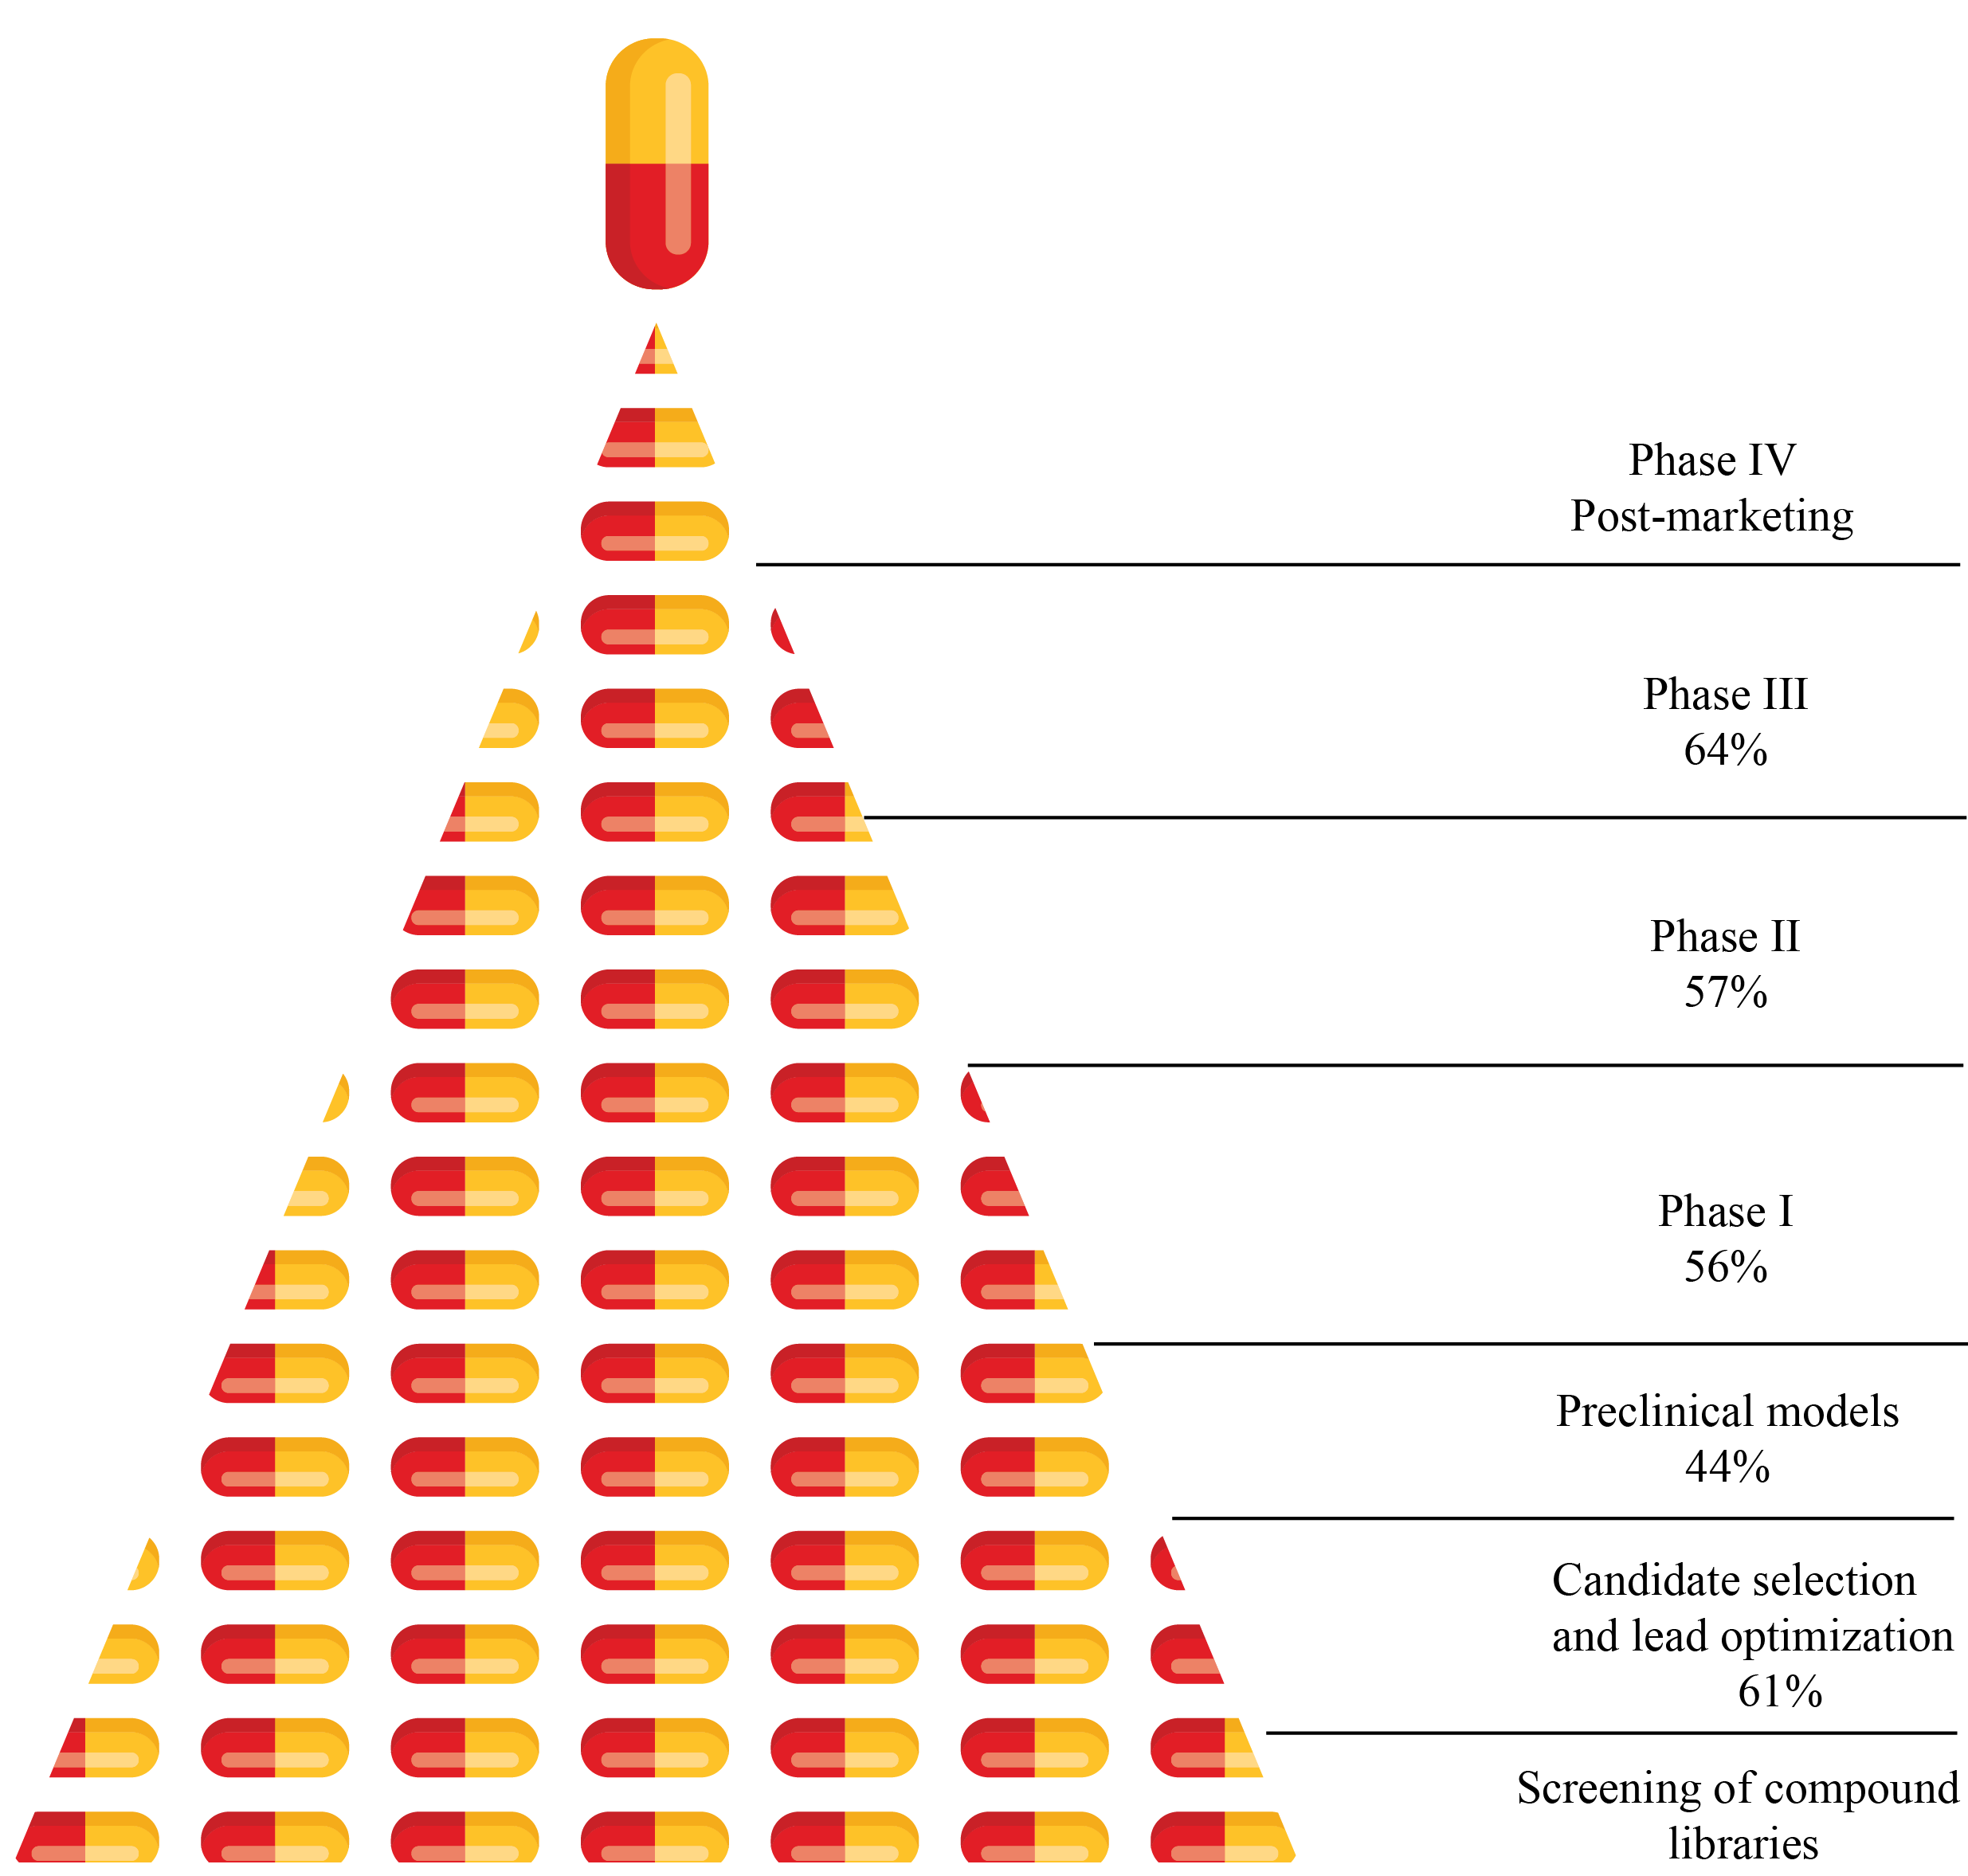
\includegraphics[width=\textwidth,height=\textheight,keepaspectratio]{Intro/ddprocess.png}%Figure from images\Figure1.png
	\caption[The 2.6 billion dollar pill.]{The 2.6 billion dollar pill. The drug development process starts with the screening of compound libraries, of which a set of leads is optimized in PK properties and safety. The candidate is further optimized in preclinical models and translated into clinical phases where the drug is tested on healthy volunteers and patients. After marketing, the drug can be withdrawn if monitoring reveals an imbalanced risk-benefit. Percentages represent the attrition rate in each phase \cite{cook2014lessons}. In total, 1 in 57 drug programs succeeds.}
	\label{fig:ddprocess}
\end{figure}
In the midst of high attrition, high cost, drug development model, biology has turned to a data-intensive field, mainly after the first sequencing of the human genome \cite{lander2001initial}. The leverage of more than 60 years of biochemical literature, combined with whole-genome, high-throughput sequencing enabled to reconstruct human biological systems \textit{in silico} \cite{duarte2007global,thiele2013community}. Metabolism being the support of biomarkers and the endpoint of the central dogma in biology, integrates the preceding genomic, transcriptomic and proteomic information \cite{mardinoglu2014genome,mardinoglu2013integration}. Modelling metabolism through Constraint-based Reconstruction and Analysis (COBRA) \cite{o2015using} allows to identify drug targets in a system-wide manner and to provide testable hypothesis thereby increasing our understanding of disease and drug action. Coupled with targeted experiments, COBRA modelling could provide a bird's-eye view on the system and drive rational drug design where in each of the steps of the drug development process, the model is further refined to answer a specific question at a given point in time.

\section{Constraint-based modelling of large scale human biological networks}
COBRA methods enable the reconstruction of human biological systems through surveying the metabolic reactions in the literature, leveraging biological data in public repositories, or performing genome-wide experiments. The set of reactions obtained are written in a mathematical format as a stoichiometric matrix $S_{(m,n)}$, where the columns are represented by $n$ reactions and the rows are the $m$ metabolites intervening in the biochemical reactions. If the obtained set of reactions is:   
\[ 
\left \{
  \begin{tabular}{ccc}
  Reaction1 & A+B $\rightarrow$ C  \\
  Reaction2 & D+E $\rightarrow$ B  \\
  Reaction3 & 2 C+D $\leftrightarrow$ E \\
  Reaction4 & B+E $\rightarrow$ C \\
  Reaction5 & A $\rightarrow$ E \\
  Reaction6 & C $\rightarrow$ A + E\\
  \end{tabular}
\right. 
\]
the corresponding stoichiometric matrix $S$ is:

\renewcommand{\kbldelim}{(}% Left delimiter
\renewcommand{\kbrdelim}{)}% Right delimiter
\[
  \text{S} = \kbordermatrix{
    & R_1 & R_2 & R_3 & R_4 & R_5 & R_6\\
    A & -1 &  0 &  0 &  0 & -1    &  1  \\
    B & -1 &  1 &  0 & -1 &  0    &  0  \\
    C &  1 &  0 & -2 &  1 &  0    & -1  \\
    D &  0 & -1 & -1 &  0 &  0    &  0  \\
    E &  0 & -1 &  1 & -1 &  1    &  1  \\
  }
\]
In the next phase, the system can be used to investigate the optimal conditions to perform a specific metabolic function, such as carbohydrate metabolism in the liver, the transport of metabolites by the intestinal epithelial cells, or a linear combination of metabolic reactions, such as the basal maintenance metabolism in the muscle. The problem becomes then a linear program (LP), in which the sought metabolic capabilities are formulated as an objective function, under a set of constraints on metabolic reactions to form the following problem:
\begin{alignat}{2}
  & \text{max or min: } &  & c^{T}_{1}v_{1}  \label{intro:eq0}\\
  & \text{subject to: } &  &  \nonumber
                \begin{aligned}[t] \\
                & Sv_{1}=b \\
                & v_{min} \leq v_{1}  \leq  v_{max}
                \end{aligned}
                \nonumber
\end{alignat}
where $c^{T}v$ is the objective function, $c$ is the vector of coefficients of the metabolic reactions in the objective function, $v$ is the vector of metabolic fluxes going through the reactions and the solution to problem \ref{intro:eq0}, $b$ is the change-of-concentration of metabolites in the considered time step, which when set to 0, the system is considered in steady-state and the solution becomes a subset of the null space of $S$ and the problem is referred to as Flux Balance Analysis (FBA) \cite{orth2010flux}. Additionally, a set of bounds are subjected on the metabolic rates of the reactions such that the allowed interval of a given reaction would be between $v_{min}$ and $v_{max}$. For example all reactions but reaction 3 are irreversible, which translates to a $v_{min} \geq 0$, while reversible reaction 3 would have $v_{min} < 0$ and $v_{max} > 0$. 
Solving problem \ref{intro:eq0} would return the optimal theoretical objective $Z_{1}$ for the system under the given constraints e.g., the maximal growth of the cancer cells in a chemically defined medium, and the solution $v$ of metabolic reactions rates achieving the objective. The flux vector $v$ would inform about the pathways involved in disease progression or drug action. 
Practically, problem \ref{intro:eq0} is often under-determined $(m<n)$, the set of solutions achieving the optimal objective is then the Alternate Optimal Solution (AOS) space. Delimiting the AOS space becomes of paramount importance in human biological models as the solutions would be reported as intervals of  metabolic rates rather than single values, thereby increasing the robustness of results. Flux Variability Analysis (FVA) \cite{mahadevan2003effects} allows the characterization of the AOS through performing two linear programs for each i\textsuperscript{th} reaction with a total of $2n$ linear programs as the following:
\begin{alignat*}{2} 
  & \text{max and min: } & & c^{T}_{i}v_{i} \\
   & \text{subject to: }&  & 
   				\begin{aligned}[t] \\
   				& Sv_{i}=b \\
   				& c^{T}_{1}v_{i}=Z_{1} \\
                & v_{min} \leq v_{i} \leq v_{max}
                \end{aligned}
\end{alignat*}
,where $c^{T}_{i}$ has one in the i\textsuperscript{th} entry and zero otherwise. The optimal objective $c^{T}_{i}v$ of minimizing reaction $i$ gives its lower bound given the optimal objective of problem \ref{intro:eq0}, while maximizing $c^{T}_{i}v$ gives the upper possible bound.
Additionally, as metabolic models increased in size to include thousands of reactions thereby covering several human metabolic pathways, the mining of information and extraction of knowledge from models becomes a challenging task. In order to select the most important metabolic reactions contributing to the emergence of a given phenotype, the sparsity induced by minimizing the 1-norm of $v$ in parsimonious flux balance analysis (pFBA) \cite{lewis2010omic}, enables a minimal set of reactions to carry flux and sets the remaining reactions to zero. Sparsity is achieved through adding a second objective in problem \ref{intro:eq0}, to minimize for the sum of flux i.e., 1-norm of $v$:
\begin{alignat*}{2} 
  & \text{min: } & & \sum_{i=1}^{n} |v_{3,i}| \\
   & \text{subject to: }&  & 
   				\begin{aligned}[t] \\
   				& Sv_{3}=b \\
   				& c^{T}_{1}v_{3}=Z_{1} \\
                & v_{min} \leq v_{3} \leq v_{max}
                \end{aligned}
\end{alignat*}
Minimizing for the 1-norm allows to obtain a reduced AOS space, which is particularly useful in the analysis of large models. Additionally, the decrease of the AOS space could be achieved through considering prior information about the state of the system. We first consider program \ref{intro:eq0}, where $S$ corresponds to the metabolic network of e.g., the liver hepatocyte with the objective set as metabolism of a given xenobiotic. After optimizing program \ref{intro:eq0}, we would like to investigate the effect of genetic mutation that would block reaction $v_{i}$, on the metabolism of the xenobiotic. We consider then the following program:
\begin{alignat*}{2} 
  & \text{max: } & & c^{T}v_{4}  \\
   & \text{subject to: }&  & 
   				\begin{aligned}[t] \\
   				& Sv_{4}=b \\
   				& v_{4,i}=0  \\
                & v_{min} \leq v_{4,[1,n] \backslash \{i\} } \leq  v_{max}
                \end{aligned}
\end{alignat*}
Similarly, we obtain an optimal objective and a set of optimal solutions. Although as liver metabolism might not be completely disrupted as an effect of mutation, and in order to make the results comparable, an additional objective would minimize the euclidean distance between $v_{4}$ and $v_{1}$. The secondary program referred to as Minimization Of Metabolic Adjustments (MOMA) \cite{segre2002analysis} is formulated as follows:
\begin{alignat*}{2} 
  & \text{min: } & & ||v_{1} - v_{4}||^{2}  \\
   & \text{subject to: }&  & 
   				\begin{aligned}[t] \\
   				& Sv_{4}=b \\
   				& v_{4,i}=0  \\
                & v_{min} \leq v_{4,[1,n] \backslash \{i\} } \leq  v_{max}
                \end{aligned}
\end{alignat*}
The obtained flux distribution would be then minimally distant and interpretable in the same context.
The above discussed methods allow to study a given system in a given point of time, to provide a snapshot of metabolism. In cases where the dynamics of the system are sought, dynamic genome-scale frameworks provide an alternative to the steady-state assumption. 
\subsection{Dynamic flux balance analysis frameworks}
The afore-mentioned methods allow to study the metabolic flux distribution of human metabolic network (FBA), assess the allowable space of AOS (FVA), potentially reducing the AOS to the most important metabolic features (pFBA) or through contextualizing the network to a prior information about the unperturbed state of the system (MOMA). While these approaches provide a snapshot of metabolism under a given set of environmental, biochemical, and genetic conditions subjected as constraints, the inclusion of the temporal dimension requires specific modelling frameworks. The study of dynamical human biological systems would inform about the dynamics of response to extrinsic perturbations in the environment and idiosyncratic properties such as modulation of gene expression.
Dynamic flux balance analysis (dFBA) has been described in the early development of COBRA methods \cite{varma1994stoichiometric}, in bioengineering applications where the growth over time of \textit{Escherichia coli} was predicted in different media. The method was formally described later and it was applied to predict the diauxic growth of \textit{Escherichia coli} in acetate and glucose \cite{mahadevan2002dynamic}, the mechanisms involving each substrate, and the subsequent shift in growth rates. There were two main approaches to simulate metabolic models dynamically, the first would solve for the entire time horizon through a terminal objective function corresponding to the final metabolite concentration, referred to as Dynamic Optimization Approach (DOA). The second is the Static Optimization Approach (SOA), where the time horizon is divided in $p$ time steps and and the metabolic model is solved in each time step. As SOA seemed to agree with experimental data \cite{mahadevan2002dynamic}, the approach has been the main implementation of dFBA. It consists of solving the metabolic model for a time step, deriving growth and uptake rates, then updating medium concentrations with the consumed and secreted metabolites, to finally compute the growth in the next time step using new availability constraints in the medium. Taking a simple model of \textit{Escherichia coli} grown on glucose, the problem would be in any given time step $t$:
\begin{alignat}{2}
  & \text{max: } & & c^{T}v_{5} 
  \label{intro:eq6} \\
   & \text{subject to: }&  & \nonumber
   				\begin{aligned}[t] \\
   				& Sv_{5}=b \\
                & v_{min} \leq v_{5} \leq  v_{max}
                \end{aligned}
                \nonumber
\end{alignat}
let $Z_{5}$ be the optimal biomass objective of problem \ref{intro:eq6}. Then the new concentration $z$ of a metabolite in the medium is:
\begin{equation}
z(t+dt)=z(t)+S^{z}v_5B.dt 
\end{equation}
,where $dt$ is the length of the time step, $S^{z}$ is the row corresponding to metabolite $z$ in the $S$ matrix, and $B$ is the biomass at this time step. Updating the availability constraints would be setting the new concentration of $z$ as the new upper bound of uptake of $z$. The metabolite concentrations time-course are actually identical to the numerical solution through Euler's forward method of:
\begin{equation}
\frac{dz}{dt}= S^{z}vB
\end{equation}
dFBA has been applied to ecosystem microbiology \cite{zhuang2011genome}, where the dynamical interaction between two bacteria were simulated using a multi-species framework named DyMMM for dynamic multi-species metabolic modelling. Later, dFBA has been used to couple a steady-state metabolic model to an ordinary differential equations (ODE) based model of external substrate dynamics. In this case, a structural set of deterministic ODEs covers a set of processes in the organism independently from the metabolic model. Coupling both model in a hybrid framework gave improved prediction of growth dynamics \cite{covert2008integrating} and set the basis for the first whole-cell integrated dynamical model \cite{karr2012whole}. The challenges faced by the bioengineering modelling community was the modelling of break points were the bacteria instantaneously shifts its metabolism when the preferred carbon source is depleted, which may cause integration failure at fixed time steps. Reducing the time step may circumvent some of the infeasibilities, yet the simulation time might increase dramatically. Direct Approaches (DA) that embed the COBRA model as a right hand side of ODEs allowed to use the common ODE numerical solvers to adapt the time step as a function of the derivative and use higher order numerical schemes to improve stability and convergence \cite{hanly2011dynamic,zhuang2011genome}. Solutions to FBA programs being non-unique and rather forming an AOS space, the dFBA programs might have different solutions depending on the LP solver, with metabolite kinetics forming production envelopes rather than a unique time-course path. The issue was addressed through adding a set of secondary objectives to select a unique solution through the dFBA lab framework \cite{gomez2014dfbalab,hoffner2013reliable}.\\
The success of dFBA was mainly validated in bacterial systems applied in bioengineering applications, and was later applied to human metabolism \cite{oyaas2017genome}. Dynamically modelling drug kinetics requires high-quality global metabolic reconstructions of human physiology. 
\subsection{Global reconstruction of human metabolism}
More than 60 years of human biochemical research produced a considerable amount of discoveries related to the function of proteins and metabolic reactions. Sequencing the human genome further developed our knowledge about gene function and essentiality. Moreover, proteins of unknown functions could be predicted using comparative genomics on the sequences and the structures, which allowed to fill the gaps in metabolic pathways. The global reconstruction of human metabolism encompassed the knowledgebase of human metabolic reactions and their encoding genes and proteins, enabling the study of a number of metabolic diseases such as Inborn Errors of Metabolism (IEM) \cite{sahoo2012compendium}, diabetes \cite{thiele2005candidate}, and the metabolic syndrome \cite{mardinoglu2014defining} \textit{in silico}. The first knowledgebase of human metabolism (Recon) \cite{duarte2007global} was built through surveying the biochemical literature and assembling 3,311 metabolic reactions encoded by 1,496 genes, into a comprehensive and stoichiometrically coherent set. The second version \cite{thiele2013community,swainston2016recon} expanded the coverage of reactions to 7,440 reactions,  2,626 metabolites, 1,789 genes, and 99 subsystems and added a number of objective functions relevant to the human physiology through a community-driven, precise protocol of high quality reconstruction generation \cite{thiele2010protocol}. Another global assembly of human metabolism was the Human Metabolic Reaction (HMR) \cite{mardinoglu2013integration,mardinoglu2014genome} reconstruction which included more than 7,000 reactions, 4,000 genes, and 3,000 metabolites.\\
Tailoring the global reconstruction through applying relevant bounds and constraints allowed to derive context-specific models such as tissue and cell type specific models \cite{schultz2016reconstruction,yizhak2014phenotype}, and a wide variety of disease models ranging from Alzeihmer's disease \cite{stempler2014integrating} to cancer \cite{folger2011predicting} and diabetes \cite{thiele2005candidate}.\\
Recently, the first model of human organ-resolved metabolism \cite{thiele2018metabolism} named Harvey after William Harvey (1578-1657), allowed to tailor the global reconstruction Recon into 20 different organs, six sex organs, and six blood cells, using human proteomic and metabolomic data and the manual curation of the organ-specific biochemical pathways, totalling more than 80,000 reactions, 50,000 metabolites, and 100 metabolic subsystems. The model connected the organs through blood circulation and accurately captured inter-organ cycles. Additionally, constraints pertaining to human physiology such as anthropomorphic parameters, human energy use, cardiac output, renal filtration rate, and gut microbiome metabolism, enables the study of a number of human disorders and the stratification of patients.\\
The global reconstruction of human metabolism provides a framework to study disease through incorporating thermodynamics, gene expression, and proteomics into context-specific models. Likewise, the study of drug effects on the human body requires the integration of COBRA models with pharmacokinetic models that describe the absorption, distribution, metabolism, and excretion of the drug.
\section{Pharmacokinetic modeling}
\subsection{Pharmacokinetic pharmacodynamic modelling (PKPD)}
The assessment of the absorption, distribution and elimination parameters of new chemical entities has been a central question in the clinical phases of drug development. Non-compartmental analysis (NCA) allows to compute the main pharmacokinetic parameters (area under the curve (\textit{AUC}), maximum concentration $C_{max}$, and $T_{max}$ which is the time where $C_{max}$ is realized ) assuming a first-order linear model. Although in cases of non-linear drug disposition and when the analysis is sought to go beyond describing the general parameters to rather predict the outcome of the next clinical phases, compartmental modelling becomes the gold standard. ODE-based models of pharmacokinetics (PK) usually describe one, two or three compartments, whose parameters are identified through fitting the model on empirical data using linear and non-linear regression. In case of low molecular weight and hydrophilic compounds, the drug is absorbed in the first compartment and immediately eliminated by a linear process (Figure \ref{fig:pkpd}-A). The compartment in this case represents the central compartment or blood. The absorption can be modelled as IV, where the total amount of the drug is immediately available in the first compartment or \textit{Per os}, where the absorption process is linear with respect to the dose following a rate of absorption $k_{a}$. The elimination can be also modelled as a linear process with rate $k_{el}$. Single compartment model equations are:
\begin{equation}
\frac{dC}{dt}=\frac{k_{a}*D}{V}-k_{el}*C 
\end{equation}
,where $C$ is the concentration of the drug in compartment 1, $D$ is the drug dose, $V$ is the apparent volume of distribution of the drug in the compartment, and $k_{a}$, $k_{el}$ are rates $(time^{-1})$ of absorption and elimination, respectively. In cases where the drug is lipophilic, it would probably bind to tissues after the absorption and exhibit a second elimination phase due to late release form deep compartments (Figure \ref{fig:pkpd}-B). The situation can be modelled as a two compartment model, where the first one idealizes the blood compartment and the second one would be the tissues where the drug binds and is slowly released thereafter. The equations of such model are:
\begin{equation} 
\begin{gathered}
\frac{dC_{1}}{dt}=\frac{k_{a}*D}{V_{1}}-(k_{el}+k_{12})*C_{1}+k_{21}C_{2} \\
\frac{dC_{2}}{dt}=k_{12}C_{1}-k_{21}*C_{2}
\end{gathered}
\end{equation}
,where $C_{1}$, $C_{2}$ are the drug concentrations is compartment 1 and compartment 2 respectively such as $C_{1}=\frac{A_{1}}{V_{1}}$, $C_{2}=\frac{A_{2}}{V_{2}}$, $A_{1}$ and $A_{2}$ are the amounts of drug, $V_{1}$ and $V_{2}$ are the drug apparent volume of distribution in compartment 1 and 2, respectively. $k_{a}$ and $k_{el}$ are as introduced previously, $k_{12}$ and $k_{21}$ are the rates of inter-compartmental diffusion from compartment 1 to compartment 2 and back, respectively. Furthermore, the elimination can be modelled as a saturable process, where liver enzymes or kidney transporters could exhibit dose-independent excretion rates. Saturation is modelled as Michaelis-Menten process, where the 2-compartment model is written as follows:
\begin{equation} 
\begin{gathered}
\frac{dC_{1}}{dt}=\frac{k_{a}*D}{V_{1}}-k_{12}*C_{1}-\frac{v_{max}*C_{1}}{K_{M}+C_{1}}+k_{21}C_{2} \\
\frac{dC_{2}}{dt}=k_{12}C_{1}-k_{21}*C_{2}
\end{gathered}
\end{equation}
,where $K_{M}$ is the enzyme constant and $v_{max}$ is the maximal rate of the enzyme.
PK models expanded beyond the classical representation to better describe the pharmacology of each compound, through adding various compartments and using different types of equations to describe physiological processes. 
\begin{figure}[!ht]
\centering
	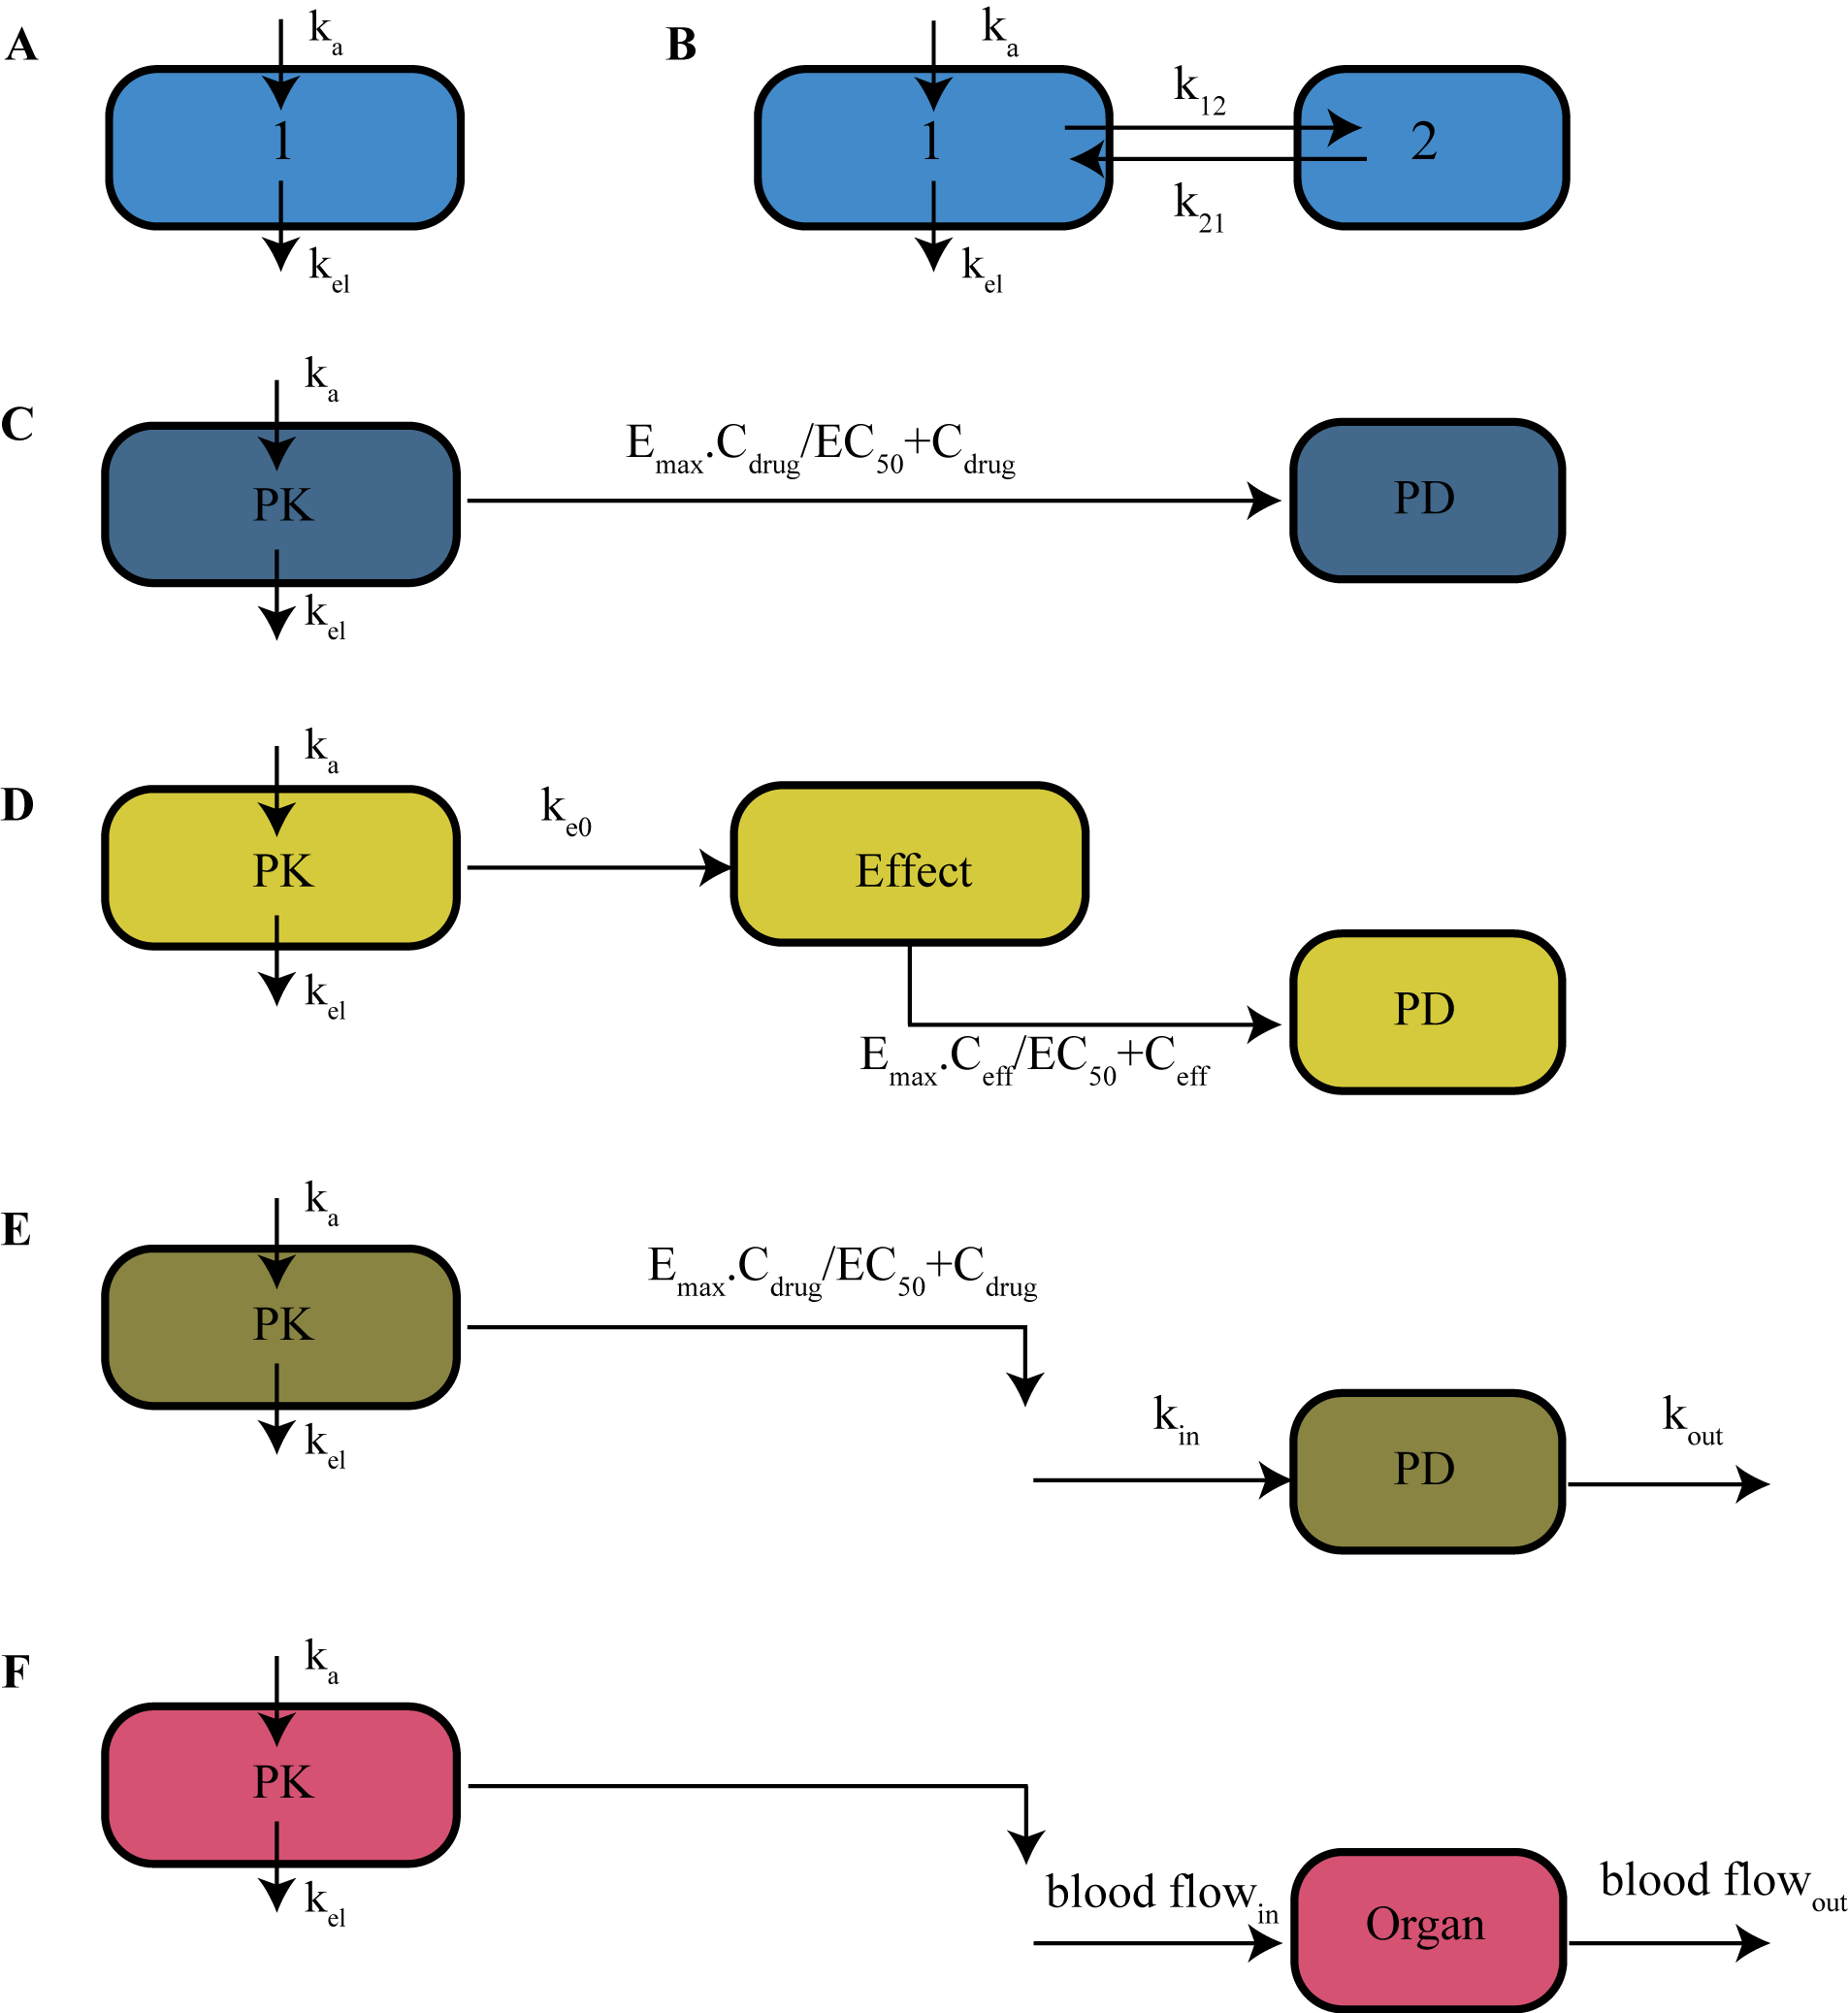
\includegraphics[width=\textwidth,height=\textheight,keepaspectratio]{PKPD/pkpd.png}%Figure from images\Figure1.png
	\caption[Different types of PKPD models.]{Different types of PKPD models. A- Monocompartmental PK model, B- Bicompartmental PK model, C- Direct effect PD model, D- PD model with effect compartment, E- Indirect effect model, F- Physiologically based PD model.}
	\label{fig:pkpd}
\end{figure}
Before the first-in-human trials, the parameters of the equations are often unknown, or at best roughly estimated through NCA. Therefore, after fitting the PK model on drug time-course concentrations in healthy volunteers, the compound parameters are estimated through non-linear regression, providing thereby a better understanding of the properties of the compounds. Oftentimes, several models are fit on the data and consequently compared on how well they explain the data through statistical metrics such as the Akaike Information Criterion (AIC) and the Bayesian Information Criterion (BIC). Model selection compares not only models of a different set of ODEs i.e., structural models, but also models with sensibly the same ODEs with slight variations. For example, in population pharmacokinetics (POP-PK), the parameters of the classical PK models can have two components, the mean population part and the individual part. Using Non-linear mixed effect (NLME) modelling, POP-PK then allows to explain between and within-individual variability to drug response. Model selection is mainly about selecting the minimal models that explain the data best. In that sense, model reduction has to be performed through eliminating correlated parameters and the inclusion of covariates such as age, sex, and weight in drug parameters. For example, the volume of distribution increases with weight, thus it can be written as following:
\begin{equation}
V= \theta + \eta*w
\end{equation}
,where $\theta$ the population mean, $\eta$ is the individual part and $w$ is the weight.  
The solution of the ODEs with the estimated parameters allows to extrapolate the PK profiles in a larger set of volunteers or patients, in order to guide later phases of clinical trials thereby enabling optimal design of experiments.
Beyond the description of pharamcokinetics, modelling provides a support to include pharmacodynamics or in other terms: what the drug does to the body. PKPD models link pharamcokinetic models to surrogate end-points e.g., the decrease of Hb1ac with anti-diabetic drugs. The pharmacodynamic effect can be modelled in various ways, depending on the delay between the administration and effect and known biology in the site of action. In cases of fast absorption and rapid distribution, the effect is observed immediately after the administration. The pharmacodynamics (PD) can be described through a direct compartment, where the drug concentrations  are directly linked to the observed phenotype \cite{upton2014basic} (Figure \ref{fig:pkpd}-C). The direct compartment is described as follows:
\begin{equation}
\begin{gathered}
E_{drug}=\frac{C_{1}}{EC_{50}+C_{1}} \\
E = E_{base}*(1-E_{drug})
\end{gathered}
\end{equation}
,where $E$ is the measured biomarker or the surrogate end point, $E_{base}$ corresponds to the basal effect prior to the administration of the compound, $E_{drug}$ is the effect induced by the drug, $EC_{50}$ is the concentration of the drug that induces half of the maximal effect and $C_{1}$ is the plasma concentration of the drug, often represented by the central pharmacokinetic compartment. In real world cases, the drug concentrations are measured as well in target organs in animal models which enables the modelling of the site of action. In many cases, the drug reaches the site of action after a certain delay as a result of slow perfusion, a signalling transduction cascade or the metabolism of prodrugs. The effect compartment has been suggested \cite{sheiner1979simultaneous} as an intermediate step between the pharmacokinetic compartment and the direct compartment. The drug concentrations from the central compartment would be subjected to a delay in the effect compartment before transducing to the direct compartment (Figure \ref{fig:pkpd}-D). If the hysteresis between the administration and the effect can be observed in the raw data, then the following effect compartment can be proposed to model the phenomenon:
\begin{equation} 
\begin{gathered}
\frac{dC_{eff}}{dt}=k_{e0}*(C_{1}-C_{eff}) \\
E_{drug}=\frac{C_{1}}{EC_{50}+C_{1}} \\
E = E_{base}*(1-E_{drug})
\end{gathered}
\end{equation}
,where the $C_{eff}$ is the concentration of the drug in the effect compartment and $k_{e0}$ is the delay parameter usually estimated from the curve fitting process as it represents the intermediary absorption and metabolism steps before reaching the site of action. The effect compartment addresses the delays caused by pharmacokinetic constraints. Likewise, in cases of delay in the pharmacodynamic processes, the indirect effect was suggested \cite{sharma1998characteristics} to model the hysteresis where the effect is neither directly linked to the central compartment nor the effect compartment (Figure \ref{fig:pkpd}-E). The indirect effect compartment is modelled as follows:
\begin{equation}
\begin{gathered}
\frac{dE}{dt}=k_{in}-k_{out}E
\end{gathered}
\end{equation}
As an example, a target protein synthesized by a zero-order rate $k_{in}$ and degraded by a first-order rate $k_{out}$ whose synthesis is stimulated by a drug, can be modelled as following:
\begin{equation} 
\begin{gathered}
\frac{dE}{dt}=k_{in}(1+E_{max}\frac{C_{eff}}{C_{eff}+EC50})-k_{out}E
\end{gathered}
\end{equation}
Symmetrically, different versions of the indirect compartment can model the inhibition and stimulation of the synthesis and degradation of the target. Generally, pharmacodynamic models exist in a wide variety of instances to describe various drug mechanisms. The pharamcokinetics of biologics for instance directly depend on their binding to the target. In this case, the pharamcodynamics drive the pharamcokinetics through target-mediated drug disposition (TMDD) models \cite{dua2015tutorial}.\\
Finally, PKPD models allow to give insights into drug effects in relation to their pharmaokinetic properties. Coupled models of pharamcokientics and pharamcodynamics allow to fit simultaneously the collected data of drug concentrations and their effect such as the target and biomarker concentration or a given clinical or physiological end point. The parameters of PKPD models are often a statistical representation that best reflect the goodness-of-fit of the model on the data. When the physiology of the system is better characterized, physiologically-based models replace the statistical parameters with mechanistic ones, thereby representing in greater detail the actual biology of the target system.
\subsection{Physiologically-based pharmacokinetic modelling (PBPK)}
PKPD models are statistical depictions of the pharmacological processes that are employed to predict drug disposition beyond the trial individuals and to guide future experiments. As such, PKPD models are rather phenomenological and lack appropriate representation of the biological system and the mechanism of drug action. In contrast, PBPK models were developed in order to go beyond the statistical representation as they integrate the known physiology of the studied system \cite{jones2013basic}. The physiological models are based on the description of human organs as compartments modelled by their weights, volume, and blood perfusion rate. Mainly used in toxicology in the beginning \cite{andersen2005introduction}, PBPK models were able to address the distribution of compounds in the different organs and assess the extent of the exposure to a given molecule \cite{peters2012physiologically}. In modelling of pharmacological agents, the PD compartments of classical PKPD model can be modified to account for known perfusion parameters in the tissue of interest giving rise to semi-physiological models \cite{wang2008preclinical} (Figure \ref{fig:pkpd}-F). The full integration of PBPK model in drug disposition uses detailed compartments of organs, where the drug absorption is modelled as following:
\begin{equation} \label{eq:PKPD}
\begin{gathered}
\frac{dC_{T}}{dt}=\frac{rate_{in}-rate_{out}}{V_{T}}\\
rate_{in}=Q_{T}C_{A}\\
rate_{out}=Q_{T} \frac{C_{T}}{K_{p}/B:P}
\end{gathered}
\end{equation}
,where $C_{T}$ is the drug concentration in the tissue, $Q_{T}$ is the blood perfusion of the tissue, $V_{T}$ is the volume of the tissue, $C_{A}$ is the arterial concentration of the drug, $K_{p}$ is the tissue to plasma partition coefficient, and $B:P$ is the blood to plasma ratio that indicates the free fraction of the drug in the plasma. The human body with its different organs modelled as compartments is represented through a generic whole-body (WB) model  \cite{peters2008evaluation} (Figure \ref{fig:s1levo}-C), that can be further expanded for the requirements of distribution of a specific drug. The basic description of each organ is based on the modelling of the in-flow of the compound through the blood perfusion, its metabolism in the organ, and the out-flow through the circulation (Equation \ref{eq:PKPD}). Additionally, several organ models \cite{poulin2002prediction,poulin2000priori,poulin2001prediction} were suggested to predict the organ-specific distribution and the concentrations of drugs in the tissue, taking into account the composition in phospholipids, neutral lipids, water, and the interstitial fraction combined with compound-specific parameters such as molecular weight, pKa, and permeability. The inclusion of these models in WB-PBPK allowed to accurately estimate the tissue to blood partition coefficient and the kinetics of the free fraction of drugs in the plasma using solely \textit{in vitro} data \cite{rodgers2006physiologically,rodgers2005physiologically,poulin2015paradigm}.
Furthermore, detailed description of the physiology of a particular system can be embedded in the WB-PBPK model such as the gastrointestinal tract that can be further compartmentalized into lumen and epithelieum as well as the different anatomical parts of the organ \cite{ando2015new,cong2000new}.\\
PBPK-PD models \cite{kuepfer2016applied} additionally include in the organ compartments the pharmacodynamics of the drug, where the drug interacts with organ specific pathways and processes. The power of PBPK models resides in the estimation of the human pharmacokinetics based mainly on \textit{in vitro} data. The \textit{in vitro}-\textit{in vivo} extrapolation (IVIVE) \cite{yeo2013application} is of paramount importance in the translation process from preclinical to clinical phases to ensure the safety of human trials \cite{lippert2012mechanistic,thiel2017comparative} and the dosing scheme for optimal efficacy. The emergence of PBPK modeling in pharmacology has been leveraged by the integration of PBPK models and simulation algorithms in software such as Simcyp (Simcyp, Sheffield, UK) , GastroPlus \cite{agoram2001predicting}, MATLAB Simbiology toolbox (The MathWorks, Natick, MA, USA), and PKSIM-MOBI \cite{eissing2011computational}. The latter is an open-source platform that enables modelling of pharmacological processes from the molecular level up to the population level.\\
Yet, in order to model organ-specific biology using ODEs, the lack of human parameters and unknown kinetics of the biological processes hinders the development of fully dynamic models. Constraint-based modelling of organ physiology using transcriptomic, proteomic, and metabolic data, can be coupled to PBPK models using dFBA frameworks to either serve as a pharmacodynamic endpoint, or to model the pharmacokinetics.
\section{Combining COBRA and PBPK}
Because of the challenges pertaining to the development of dynamic genome-scale models \cite{gilbert2017towards}, hybrid models of biological systems that encompass continuous (ODE) and discrete (FBA) behaviour, have been described in bacteria \cite{covert2008integrating,karr2012whole}, and paved the way towards kinetic genome-scale models. Combining two formalisms has the advantage of increasing the coverage of reactions, metabolites and phenotypic prediction, in addition to the temporal dimension (Table\ref{tbl:pbpkvscobra}). Moreover, additional constraints can arise from the combined model, thereby reducing the space of possible phenotypes to biologically relevant ones. Recently, the approach have been applied to human physiology through the integration of human hepatocyte metabolic model with an ODE-based PBPK model of allopurinol \cite{krauss2012integrating} to investigate the effect of enzymopathies on ammonia detoxification in the liver and the reduction of uric acid production following allopurinol treatment. Hybrid PBPK-COBRA models \cite{conde2016constraint,maldonado2017integration} were also applied in the study of phenytoin and estradiol drug-drug interaction \cite{sier2017linking}. Combined PBPK and COBRA models are anecdotic, but we expect their number and applications to extend in the community with the development of methods and tutorials.
There are two ways of constructing hybrid, bi-formalism models.

\begin{table}[h]
\caption[Comparison of PBPK models with metabolic models.]{Comparison of PBPK models with metabolic models.}
\begin{center}
	\begin{tabular*}{\textwidth}{l @{\extracolsep{\fill}} lll}
	\hline
	Model	   & PBPK                     & COBRA \\ 
	\hline
	Coverage   & a few metabolites        & genome-scale \\
	Dynamics   & dynamical                & steady state \\
	Prediction & quantitative             & semi-quantitative \\
	Parameters & many                     & few \\
	Concept    & Top-down (curve-fitting) & Bottom-up (network reconstruction) \\
	\hline
	\end{tabular*}
\end{center}
\label{tbl:pbpkvscobra}%descriptive label to refer to figure in text
\end{table}

\subsection{COBRA as pharmacodynamics - horizontal coupling}
The foundations of systems pharmacology were built on the promise of integration of systems biology models as pharamcodynamic endpoints in PKPD models \cite{iyengar2012merging,danhof2016systems}. Pharamcodynamics defined as `what the drug does to the body` would link drug concentrations to the surrogate end point and would be represented in PKPD models through phenomenological equations. Coupling COBRA models as pharmacodynamics in PBPK-PD models implies that the PK of the drug is deterministic for the entire simulation time. The coupling is considered hierarchical as concentrations from the PK compartment will shift the states of the COBRA model through time e.g., the detoxification of ammonia using a genome-scale network of the hepatocyte \cite{krauss2012integrating}. Also referred to as indirect coupling \cite{krauss2012integrating}, the method requires the identification of contact points between the PBPK-PD model and the COBRA model. Assuming that reaction $R1$ is modeled in both the PBPK and COBRA model, the method consists of solving the ODEs for each time step and subjecting the derivative terms as constraints in the metabolic model. In the PBPK model, the concentrations of metabolite $M$ are determined by a production term $v_{d,R1}$ and consumption terms $v_{d,R2}$ and $v_{d,R3}$ such as the following:
\begin{equation} \label{intro:eq1}
\frac{dM}{dt}=Mv_{d,R1}-Mv_{d,R2}-Mv_{d,R3}
\end{equation}
,where $d$ stands for dynamic.
The COBRA model is dynamically constrained for each time step and $Mv_{d,R1}$ is set as a bound in the counterpart of $v_{d,R1}$ which is $v_{m,R1}$, where $m$ stands for metabolic.
\begin{alignat*}{2}
  & \text{max or min: } &  & c^{T}v_m\\
  & \text{subject to: } &  &  
                \begin{aligned}[t] \\
                & Sv_{m}=b \\
                & v_{m,R1} \leq,=,\geq Mv_{d,R1}\\
                & v_{m,min} \leq v_{m}  \leq  v_{m,max}
                \end{aligned}
\end{alignat*} 
In most cases, the rates of absorption of the drug and its metabolites would be the most straightforward flux to couple. The PBPK-PD endpoint could be a signalling cascade involving metabolic enzymes, whose concentrations could set the upper bounds in COBRA models. While the coupling will preserve the pharmacokinetic profile of the drug, the COBRA model would have several states induced by dynamically changing the bounds of reactions in FBA programs, thereby tracking the activation of metabolic pathways over time, as an effect of the drug (Figure \ref{fig:couplings}-A). 
\subsection{COBRA as pharmacokinetics - vertical coupling}
\begin{figure}[!htp]
\centering
	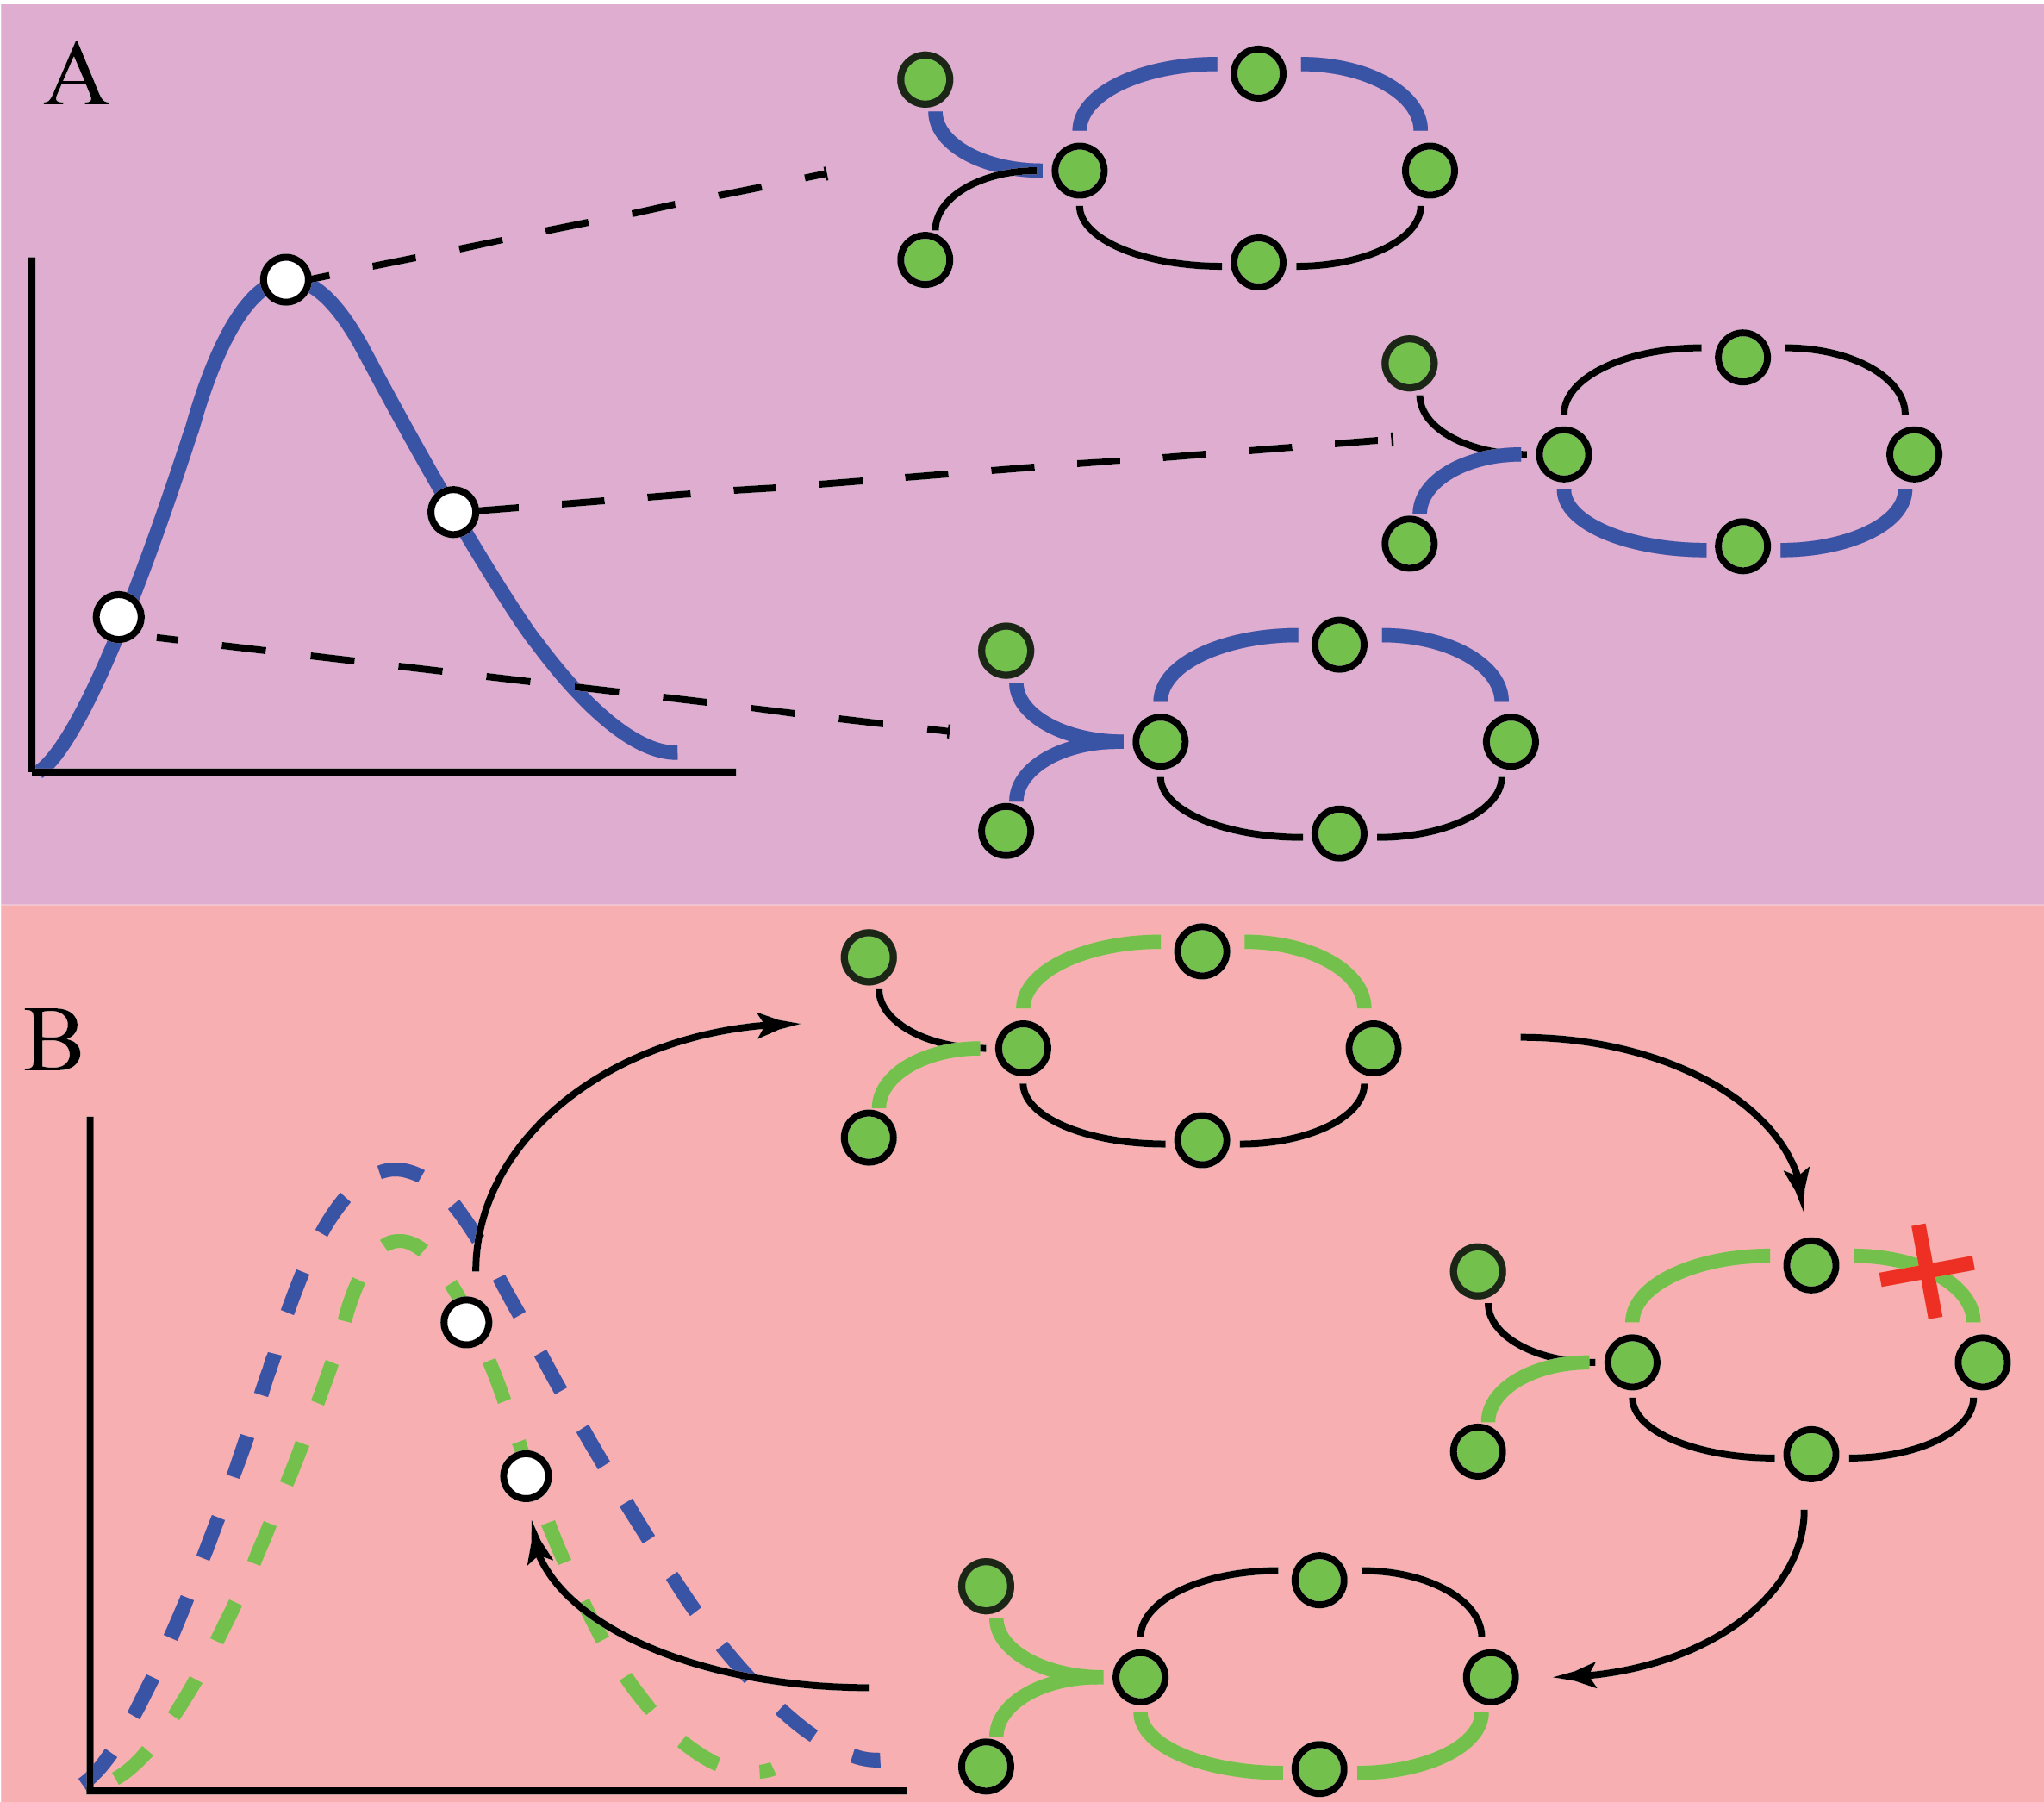
\includegraphics[width=\textwidth,height=\textheight,keepaspectratio]{Intro/couplings.png}%Figure from images\Figure1.png
	\caption[Coupling PBPK and COBRA models.]{Coupling PBPK and COBRA models. A– Horizontal hierarchical coupling consists of solving the PBPK model first in discrete time steps and subjecting reaction rates as constraints in the COBRA model to track the metabolic shift in the network as an effect of drug constraints. Depending on the research question, reaction constraints can be set as lower or upper bounds. B- Vertical coupling assumes a cross-talk between both models. As such the PK profile of the drug is not determined by the ODEs alone. In the first step, after solving the PBPK model, the derivatives are applied as constraints in the COBRA model. Additional constraints are set to represent a specific condition that is not captured by the ODE, such as enzymatic deficiency. The COBRA model is solved to obtain a solution satisfying the constraints. Finally, derivative terms in PBPK corresponding to reactions in the COBRA model solution are set accordingly and the PBPK model is integrated for the next time step. The PK of the drug obtained from the PBPK model is drawn in blue and its new PK constrained by the PBPK-COBRA model is represented in green.}
	\label{fig:couplings}
\end{figure}
Practically, hierarchical coupling would require more than one constraint to induce a shift in the steady state of the COBRA model. Since PBPK models describe usually the drug and its metabolites, additional constraints arising from gene expression experiments or metabolomics could be added to further inform the model \cite{willemsen2015metdfba}.\\
When drug pharmacokinetics are modulated by the COBRA model, as in the case of a decrease in the drug metabolising enzyme (DME) activity in the liver, enzymopathies, or in cases where the interaction with the target influences the PK as in TMDD, the coupling would be direct.
To illustrate the method, let us consider the previous PBPK model and a COBRA model sharing reaction $R1$. Solving the ODEs in the first time step allows to compute the term $Mv_{d,R1}$ corresponding to the flux of $R1$. In the COBRA model, $Mv_{d,R1}$ is set as an upper bound in the counterpart of $v_{d,R1}$ which is $v_{m,R1}$. Additional constraints could be added, such as blocking $v_{m,R6}$ to model an enzymopathy.
\begin{alignat}{2}
  & \text{max or min: } &  & c^{T}v_{m}  \label{intro:eq2}\\
  & \text{subject to: } &  & \nonumber
                \begin{aligned}[t] \\
                & Sv_{m}=0 \\
                & v_{m,R1} \leq Mv_{d,R1} \\
                & v_{m,R6} = b \\
                & v_{m,min} \leq v_m \leq  v_{m,max}
                \end{aligned}
                \nonumber
\end{alignat} 
Solving problem \ref{intro:eq2} allows to obtain $v_{m,R1}$ which sets a new value for $v_{d,R1}$ under the specified enzymopathy constraints and the ODEs \ref{intro:eq1} are integrated for the next time step.\\
The concentration time-course of the drug in the hybrid model is different from the PK profile predicted by the set of ODEs alone (Figure \ref{fig:couplings}-B). The method was described in the prediction of ammonia detoxification in patients presenting urea cycle disorder \cite{krauss2012integrating}, where the PBPK model described the PK processes of ammonia combined with a COBRA model of the hepatocyte whose ornithine carbmylase flux was gradually decreased to describe the progression of the disorder, allowing the prediction of  the PK of ammonia in patients. Another coupled model predicted alcohol concentration in volunteers who presented different alcohol dehydrogenase enzyme activity \cite{toroghi2016multiscale}. In type 1 diabetes (T1D), a PBPK model of glucose-insulin-glucagon interplay was coupled to a multi-cellular model of a myocyte, hepatocyte and adipocyte, where the impairment of T1D-related genes influenced the time-course of glucose \cite{wadehn2016multiscale}.   
We applied this approach to predict the gastrointestinal absorption of levodopa under dietary constraints wherein the presence of amino acids would induce either luminal competition or basolateral trans-stimulation, which gave rise to complex PK profiles depending on the diet composition and the time of intake \cite{guebila2016model}.
As the models include several organs and describe several metabolic processes, the issue of the non-uniqueness of solution and the non-smoothness of PK profile have been addresses through reducing the AOS space with a secondary objective (pFBA) \cite{toroghi2016multi}.\\
Taken together, COBRA models can extend the pharmacodynamics of PBPK models through a genome-scale coverage of metabolites and reactions. They alternatively can be used to predict the kinetics of the drug under new constraints arising from cellular processes such as enzymopathies. 
The inclusion of PKPD modelling, constraint-based modelling, and hybrid models under the umbrella of systems pharmacology \cite{van2011systems} has the potential to leverage the drug development process through increasing our understanding of disease pathophysiology and drug mechanism.
\section{A new drug development paradigm}
The target discovery and drug development process has been through several paradigm shifts. In the second half of the twentieth century, target discovery in the preclinical stage was driven by empirical observation on animal models, where a set of compounds were screened on disease animal models such as cancer. Rodents carrying patient-derived tumour xenograft were tested for a number of compounds and the dose was selected through titration methods. If the xenograft shrinks in size, then the compound had higher chances of translation into the clinical phases with little known about its mechanism and the reasons of success or failure. Later, the advent of crystallography and the availability of cytoplasmic and transmembrane protein structures that formed the majority of drug targets, allowed the development of the key-lock paradigm \cite{medina2013shifting}. Small molecules that fit in specific binding pockets of target proteins to induce a stimulatory or inhibitory effect, were designed through docking experiments. Computer-aided drug design and molecular dynamics are a powerful tool towards rational and optimal drug design. Nonetheless, this target-centric approach failed in considering the biological system as a whole and the selective inhibition of important signalling hubs induced long lasting side effects. Notably, Cyclooxygenase 2 (COX-2) inhibitor Rofecoxib indicated as an-inflammatory agent induced high risk of heart failure and provoked up to 30,000 deaths post-marketing between 1999 and 2004 \cite{juni2004risk}. At the same time, biology and pharmacology became data-intensive disciplines following the development of sequencing techniques \cite{lander2001initial} and the availability of data in public databases. The post-genomic drug discovery and development process has to build on known biology and fundamental science through integrating the different layers of information into convergent, hypothesis-free models of the target system \cite{van2016taking}. In line with recent calls to build model-based drug-development process by regulators \cite{us2004innovation} and by academics \cite{oberhardt2013metabolically,van2011systems}, we propose a novel drug discovery and development paradigm that builds context-specific dynamical metabolic models of human disease through transforming publicly available data into queriable knowledgebases. In the following, I will detail the vision entailed by a novel, data-intensive, model-based drug development process (Figure\ref{fig:newparadigm}) and provide examples applicable in preclinical and clinical phases using the work I carried during the course of my PhD.
\subsection{Preclinical phase}
\subsubsection{Disease signatures as targets}
The main outcome of sequencing technologies in human disease was the discovery of single nucleotide polymorphisms (SNPs) related to disease using thousands of genome wide sequences of healthy individuals and patients. Yet, GWAS studies showed that i) most of these SNPs were in non-coding regions of the genome wherein a small number of diseases could be linked to the change of sequence or structure of an enzyme, and ii) they were able to provide disease signatures. Specifically, disease signatures correspond to the gene expression profile in a given condition. Similarly, drug-induced gene expression experiments provided the gene expression related to a perturbation induced by a small molecule. Notably, the connectivity map \cite{lamb2006connectivity,subramanian2017next} has over 1.7 million \textit{in vitro} drug and drug-like induced gene expression profiles in different cell types, at different doses and different time points. Conceptually, if the drug-induced gene expression profile reverses the gene expression induced by a disease, then it can be a potential candidate for further development. For example, the reverse transcription concept has been used to treat dyslipedimia in mouse models \cite{wagner2015drugs} and repurpose drugs in nephropathy \cite{zhong2013renoprotective} and in small cell lung cancer \cite{jahchan2013drug}. Particularly, it presents a potential avenue for repurposing the existing drugs on the market for new indications \cite{dudley2011exploiting}. The clinical phase would then start directly in phase two, accelerating considerably the process and reducing the costs. Using molecules existing in the market allows to use the post-marketing safety data to reduce the amount of clinical experiments performed.
Moreover, building context-specific metabolic models of drug and disease through combining gene expression with biochemical networks allows to get insight into the phenotype of interest and predict metabolic biomarker thereby providing a rationale for the optimal design of experiments. 
\subsubsection{Target-free drug repurposing and reclassification}
The current drug classification system is based on the indication and the chemical class of the compound. The indication of the drug is oftentimes suggested prior to the beginning of the drug development program. If the drug proves to be active towards the clinical indication then it will be classified in the family of compounds that have similar activities such as the antibiotics class and the antidepressants class. Although in reality, small molecules have more than one activity. The current classification is biased towards the indication tested and intended for in the preclinical phase. The repurposing of Sildenafil and Minoxidil in erectile dysfunction and hair loss respectively, showed that a given drug could be moved from one class to the other as in case of Minoxidil from a hypotensive agents to a dermatological agent. The classification of drugs has to take into account their molecular, genetic and biochemical profile. Such classification will enable to use compounds in the same class exchangeably in similar indications, thereby harnessing drug repositioning efforts. We applied this concept to reclassify drugs with respect to their gastrointestinal effects. The drug-induced gene expression profiles from the connectivity map \cite{subramanian2017next} were used to tailor generic small intestine epithelial cell models to represent the drug action on the gut wall. Then, we clustered drugs with similar metabolic profiles into sets that had a similar genome-wide fingerprint (Chapter \hyperref[ch:chapter2]{2}). Notably, the clusters did not match the usual drug classes as currently reported by medicine agencies.
\subsubsection{Prediction of gastrointestinal side effects}
Metabolic modeling combined with machine learning was applied in the prediction of drug iatrogenic effects. Using drug induced gene expression data \cite{subramanian2017next} and reported drug target \cite{knox2010drugbank}, context-specific models informed about disrupted metabolic pathways \cite{zielinski2015pharmacogenomic}, and accurately predicted the occurence of adverse reactions \cite{shaked2016metabolic}.\\
Since the oral absorption of drugs is the most common route of administration, gastrointestinal side effects are the most frequent adverse reactions. They can induce a lower compliance to the treatment and sometimes cause the treatment to stop. The accurate prediction of gastrointestinal side effects in the preclinical phase, based solely on \textit{in vitro} data can provide invaluable information about the safety of the compound and guide the decision to proceed with clinical phases. Using the connectivity map drug gene expression profiles \cite{subramanian2017next}, we built drug-constrained metabolic models of the gastrointestinal epithelium of FDA approved drugs (Chapter \hyperref[ch:chapter2]{2}). We developed a machine learning classifier that linked drug genetic and metabolic profiles to the induced side effects as reported in the SIDER database \cite{campillos2008drug} and their mechanism of action as reported by the FDA National drug code directory (NDCD). We showed that the accuracy of prediction improved in comparison to approaches that use gene expression alone. We concluded in this work, that context-specific models of metabolism, in addition to gene expression, taken as features in a machine learning classifier could accurately predict adverse reactions.\\
The integration of multi-layer biology of genetic and metabolic signatures is a powerful tool to assess the clinical symptoms induced by xenbiotics in the preclinical phase. Moving towards the clinical phases, the translation of preclinical discovery to human has been equally in addressed in the context of PBPK models \cite{thiel2017towards} and metabolic modeling \cite{blais2017reconciled}. A consensus rat and human model \cite{blais2017reconciled} allowed to highlight species metabolic differences and to predict biomarkers to 76 drugs enabling thereby the translation of preclinical findings to clinical phases. 
\begin{figure}[!ht]
\centering
	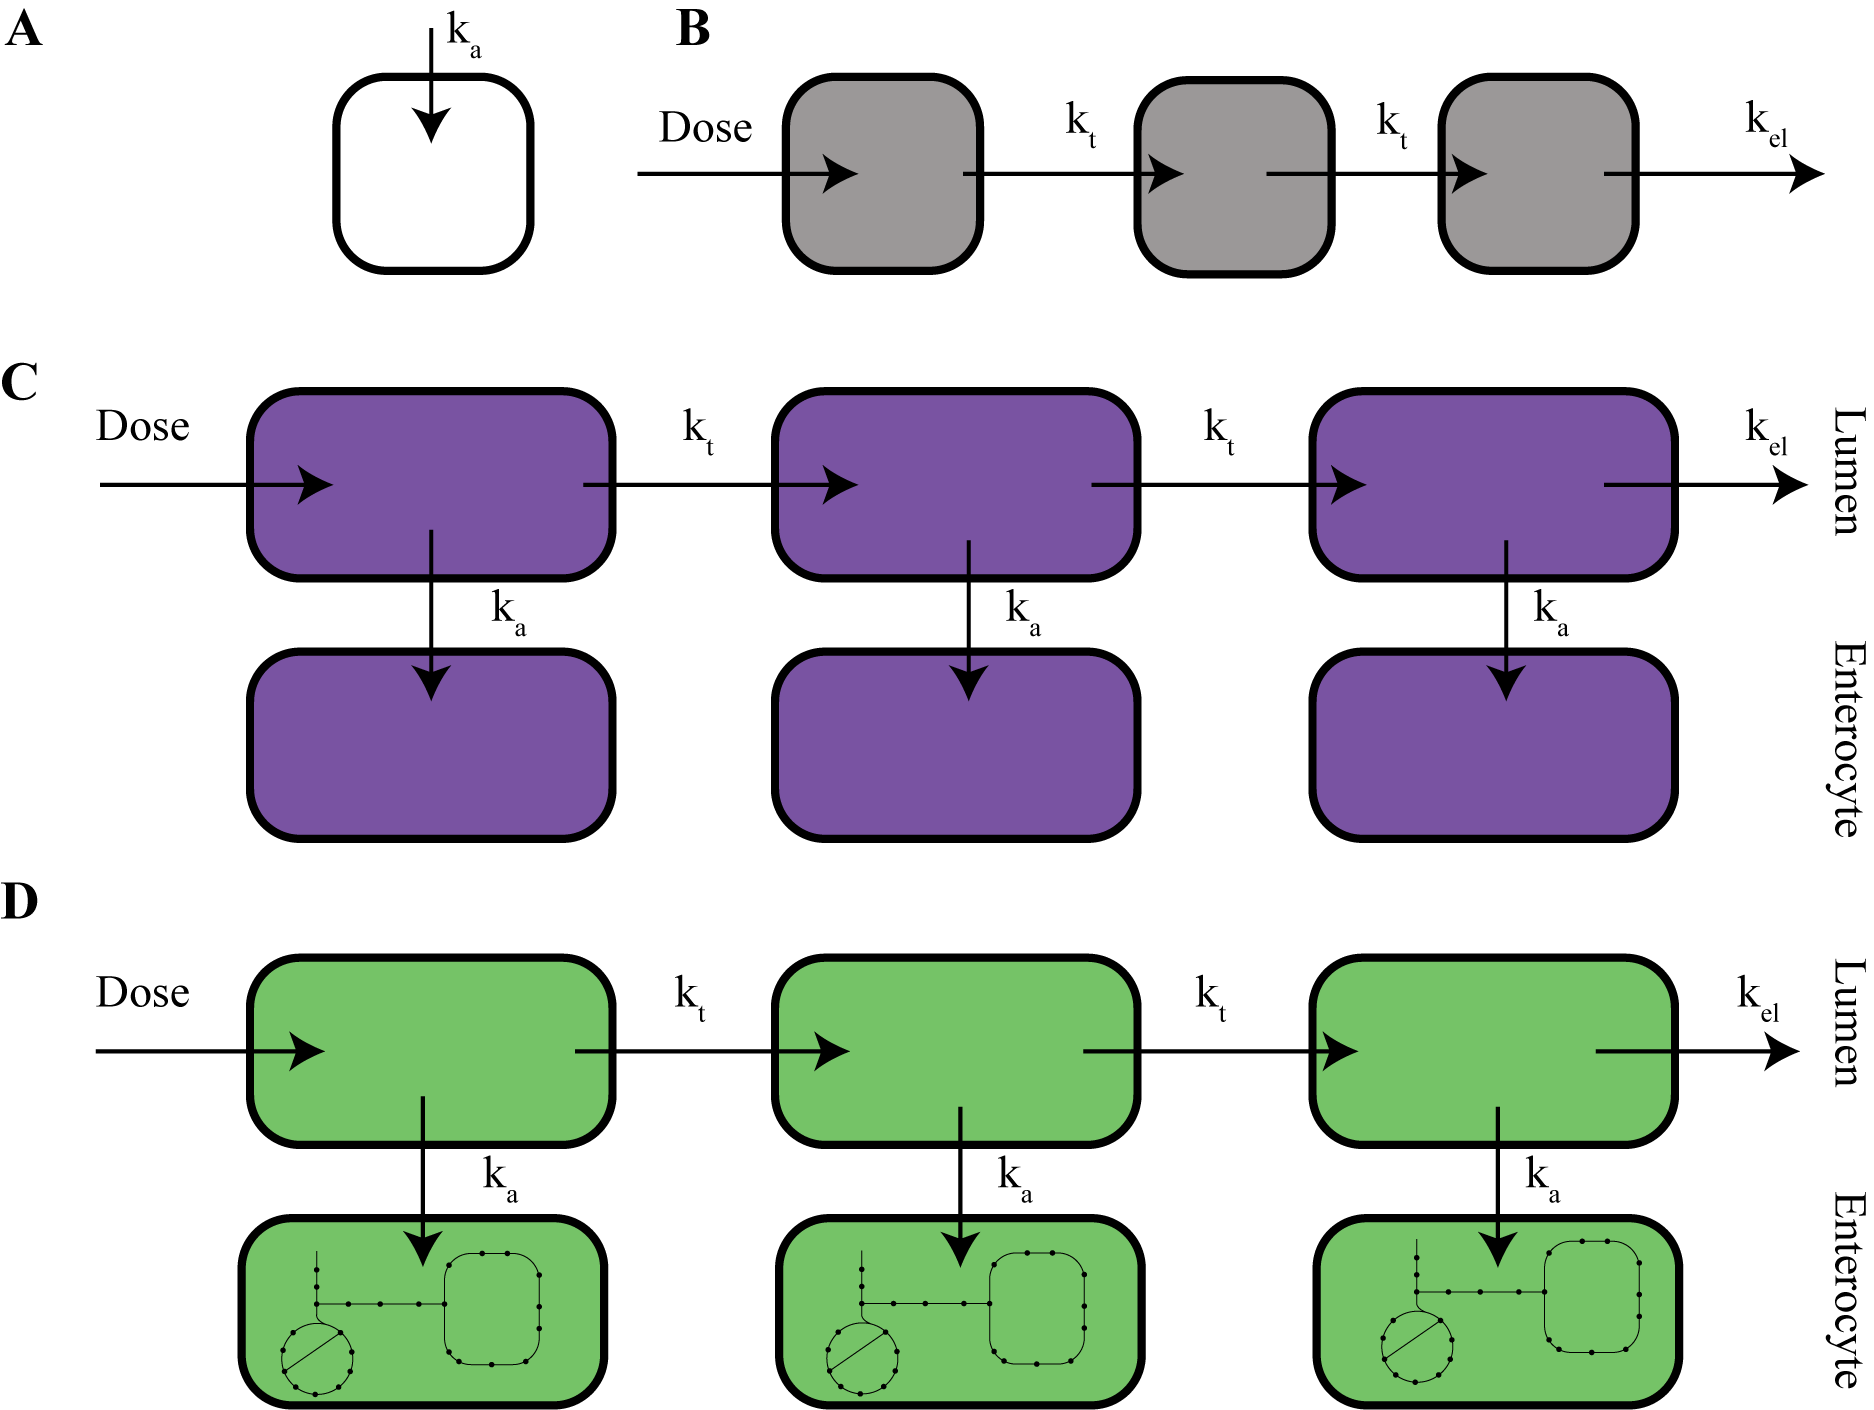
\includegraphics[width=\textwidth,height=\textheight,keepaspectratio]{ACATEVO/acatevo.png}%Figure from images\Figure1.png
	\caption[Evolution of absorption models in pharmacokinetic modeling.]{Evolution of absorption models in pharmacokinetic modeling. A- Monocompartmental PK model, B- Compartmentalized absorption and transit (CAT) model taking into account anatomical sections of the gastrointestinal tract. C- Advanced compartmentalized absorption and transit (ACAT) absorption, dissolution, and transit model. D- Small intestine epithelial cell (sIEC)-ACAT systems pharmacology model.}
	\label{fig:acatevo}
\end{figure}
\subsection{Clinical phase}
\subsubsection{Improving the bioavailability of Levodopa}
Metabolic modeling was applied in the prediction of the effects of the most commonly used marketed compounds \cite{sahoo2015modeling}. In early clinical phases, the compound is tested for potential interactions with other drugs and diet in order to optimize its efficacy and derive recommendations. As the lack of efficacy is one of the major reasons for the failure of drug development programs, we developed a gastrointestinal model to study the efficacy of a drug-diet interaction, namely levodopa and amino acids \cite{guebila2016model}. Levodopa is a supplementation therapy in Parkinson's disease, which is caused by the decrease of the amount of dopamine produced in the brain as an effect of the loss of dopaminergic neurons. The supplementation of the precursor of dopamine, levodopa, allows to restore the normal levels of dopamine in the brain. Levodopa has a similar chemical structure to amino acids, thereby it competes for absorption in the blood brain barrier and the gut wall. It is recommended for patients to avoid amino acid-rich diet to maintain the efficacy of the drug and decrease the 'on-off' phenomenon where a patient exhibits akinetic phases followed by dyskinesia. Although, the absorption of levodopa in the blood brain barrier is well documented, its transport in the gut wall was assumed to happen in a similar fashion. Recently, novel transporters of levodopa in the gut wall were identified \cite{camargo2014molecular}, which provided novel insights about the concomitant absorption of levodopa and dietary amino acids. As steady state metabolic models cannot address time-dependant phenomena, we developed a multi-scale dynamical model (Figure \ref{fig:acatevo}-D) of the absorption of levodopa along the gastrointestinal tract and we embedded a genome-scale model of the small intestine epithelial cell in the gut compartments to account for the molecular interaction between the drug and diet. We showed the mechanism beyond successful empirical dietary recommendations and provided a novel model-based diet for Parkinson's disease patients. We classified amino acids by their synergistic ability towards levodopa absorption. A recent clinical trial \cite{nagashima2016effects} showed that the absorption of levodopa was improved when soybeans were administered concomitantly, which confirmed several aspects of our hypothesis.\\
This example particularly showed the importance of the modeling-experiment loop in drug development \cite{krauss2017translational,kuepfer2012multiscale}, where the simulations integrate new findings and guide future experiments, that in return, validate the predictions and calibrate the model.
\begin{figure}[!htp]
\centering
	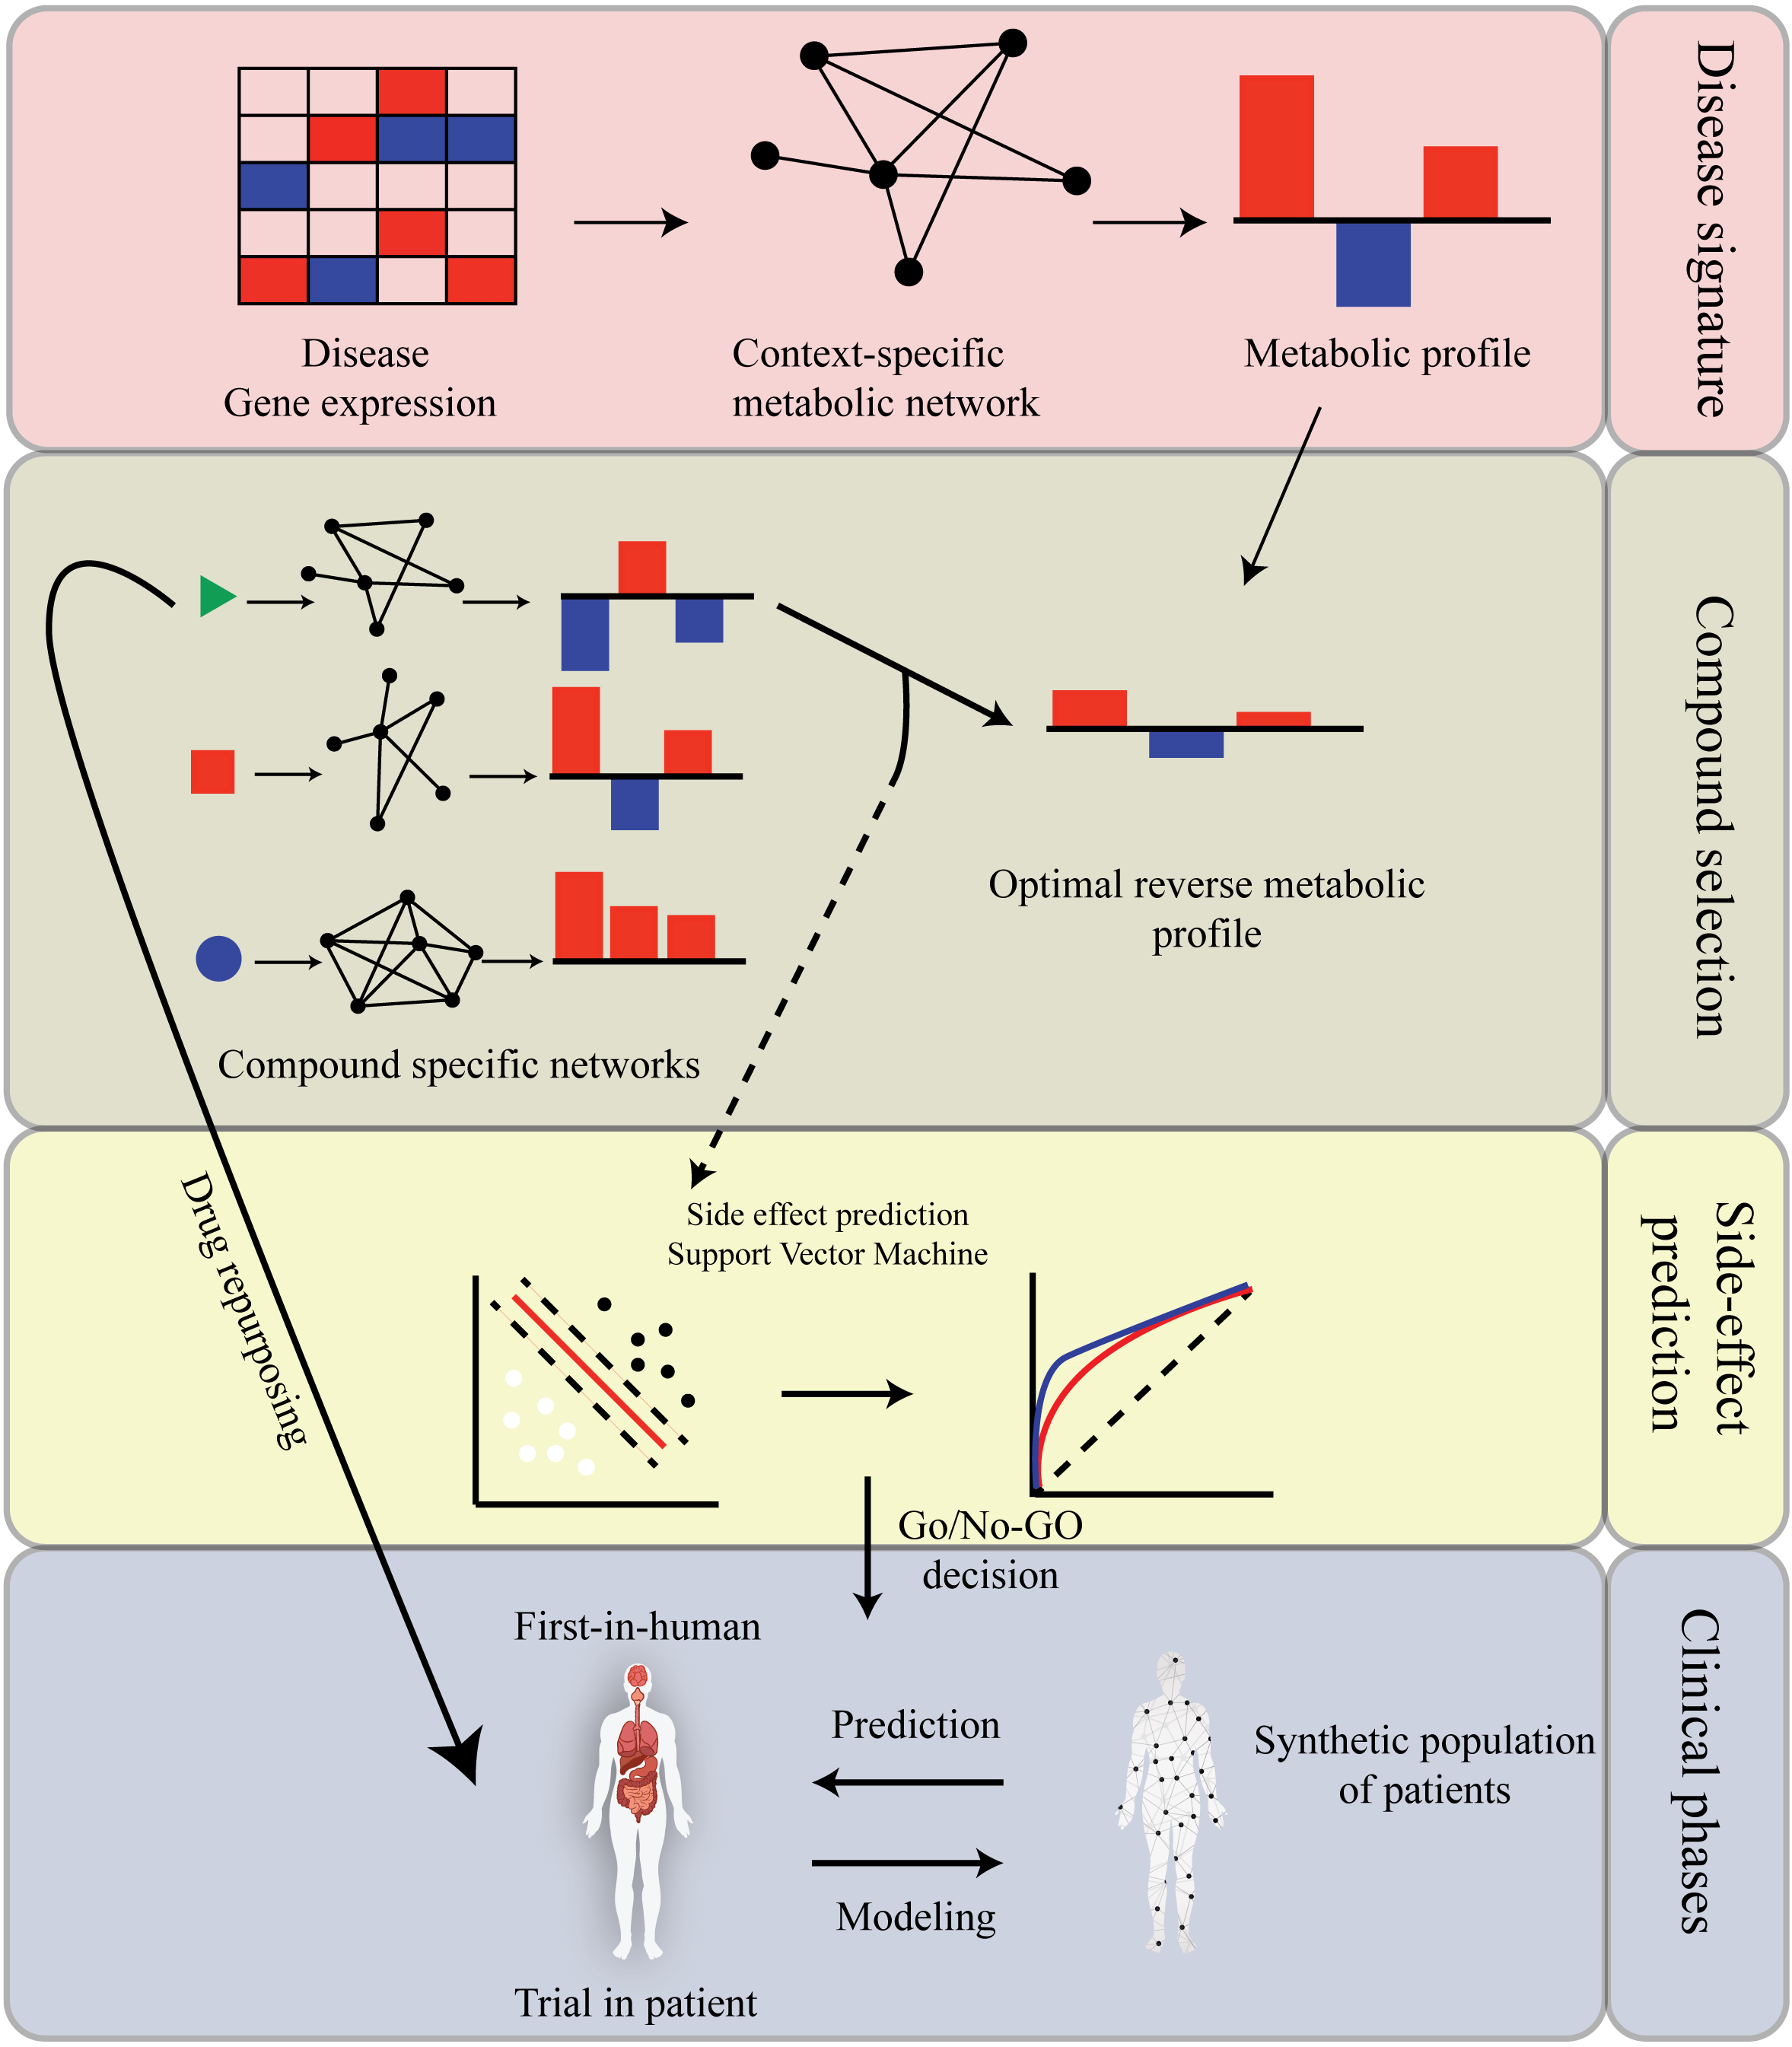
\includegraphics[width=\textwidth,height=\textheight,keepaspectratio]{NewDrugDevelopment/DrugDevPipeline.png}%Figure from images\Figure1.png
	\caption[A new drug development paradigm.]{A new drug development paradigm. Using known biology and publicly available databases, integrative disease models are built to describe the multi-layer biology of the disease. Instead of optimizing the compound for its binding affinity to a specific target, the compound is optimized for its ability to reverse the disease network state. Drug signature networks are built in a similar fashion to disease networks and compounds that reverse the systemic fingerprint of the disease are selected for further development in a target-free manner. If the small molecule exists in the market then it is moved to phase II clinical trials and repurposed for the current indication. Otherwise, the compound efficacy and safety are assessed through querying side effect databases and performing animal experiments to support the decision to move to the clinical phases. In clinical phases, an iterative approach combining empirical observation on patients and healthy individuals and the modelling of synthetic populations to guide further experiment.}
	\label{fig:newparadigm}
\end{figure}
\subsubsection{Assessing between- and within-patient response to insulin}
In later clinical phases, where the trials are expanded to a great number of participants to include several anthropomorphic groups of healthy individuals and patients, the variability of response is a major outcome of population studies which can lead to the stratification of patients through adapting the dose or deriving counter-indication for non-response groups. At this stage, clinical and molecular information about the drug is available and enables the modeling of drug pharmaockinetics in disease models \cite{danhof2015kinetics,kuepfer2010towards}. Furthermore, it can guide the large-scale experiments through modelling synthetic populations of patients. We considered type 1 diabetes as an example for this concept. Type 1 diabetes is caused by the decrease of insulin-producing cells in the pancreas, thereby causing a deregulation of the glucose-insulin-glucagon system. The onset of the disease takes place at early stages of life and requires constant supplementation of insulin to restore glucose levels. The variability of response between and within the same individual requires a constant monitoring and adaptation of the dose in addition to high socio-economical burden coming from frequent doctor visit. Type 1 diabetes being a systemic disease, we integrated a whole-body metabolic model with a dynamical model of glucose-insulin-glucagon system \cite{schaller2013generic}, gene expression data measured in T1D patients as well as the concentration time-course of key metabolites induced by insulin to build an integrated model of type 1 diabetes. We used the model to simulate a population of T1D patients and derived factors underlying inter and intra-individual variability (Chapter \hyperref[ch:chapter5]{5}). Additionally, we compared the metabolic signature of T1D to existing drug signatures and hypothesized a set of molecules as adjuvants in insulin therapy.\\
Taken together, as models of biological systems are increasing in scope and size \cite{goldberg2018emerging}, the integration of genome-scale hybrid dynamical models in all steps of the target discovery, preclinical trials, first-in-human trials to the assessment of drug-drug and drug-food interactions can leverage the drug development processes. The emergence of system-based design of therapies can optimize the outcomes and ensure higher success rates.
\section{Scope and aim of the thesis}
The project described in this thesis was built on four main objectives. First, to predict the gastrointestinal side effects of drugs based solely on \textit{in vitro} data and to classify drugs with respect to their metabolic and transcriptomic signature. Second, to predict the efficacy of levodopa under different dietary schemes using a dynamical genome-scale model of the gastrointestinal tract. Third, to design efficient computational methods in metabolic modelling to allow the simulation of large-scale metabolic models. Last, to upscale the combined models of genome-scale metabolism (COBRA) and drug disposition (PBPK) from the gastrointestinal tract to whole-body level. \\
Efficacy and safety being the two major reasons for the failure of drug development programs, I addressed the safety of compounds in the first part using drug-induced gene expression to derive context-specific models of the gut wall. I used the features of the metabolic models to predict gastrointestinal side effects and to classify drugs with respect with their metabolic and gene expression signature rather than by their indication (Chapter \hyperref[ch:chapter2]{2}). In the second part, I addressed drug efficacy with respect to a drug-food interaction specifically to optimize the gastrointestinal bioavailability of levodopa through optimizing diet using a hybrid PBPK-COBRA model (Chapter \hyperref[ch:chapter3]{3}). The third part surrounds the design of fast software for the simulation of large-scale metabolic models (Chapter \hyperref[ch:chapter4]{4}), which allows the upscaling of the combined models of metabolism and drug disposition to whole-body level. The whole-body model allowed to assess the between and within-patient variability to insulin action (Chapter \hyperref[ch:chapter5]{5}).  A brief description of the chapters and the individual contributions is provided in the following section.\\

\noindent {\large \textbf{Chapter 2: \hyperref[ch:chapter2]{Predicting gastrointestinal drug effects using contextualized metabolic models.}}}\\
\noindent Chapter \hyperref[ch:chapter2]{2} describes the prediction of gastrointestinal side effects using a statistical classifier based on \textit{in vitro} drug-induced gene expression and \textit{in silico} predicted gut wall metabolism. Then, we used genetic and metabolic features to go beyond the indication-based classification of drugs to assess compound similarities. The gut wall metabolic model was later used to assess the efficacy of the gastrointestinal absorption of levodopa (Chapter \hyperref[ch:chapter3]{3}]).
\subsubsection{Contributions}
Marouen Ben Guebila (M.B.G.) and Ines Thiele (I.T.) wrote the manuscript, M.B.G. designed the study and carried the analysis. I.T. supervised the project.\\

\noindent {\large \textbf{Chapter 3: \hyperref[ch:chapter3]{Model-based dietary optimization of late-stage, levodopa-treated, Parkinson's disease patients.}}}\\
\noindent Chapter \hyperref[ch:chapter3]{3} addresses the bioavailability of levodopa when co-administered with different types of nutritional schemes. The small intestine COBRA model was combined with a dynamical model of levodopa dynamics in the intestine (ACAT model). The combined model allowed to provide a mechanism-based diet to improve the efficacy of levodopa, which was in agreement with a recent clinical trial \cite{nagashima2016effects} . The results were published in NPJ systems biology and applications in June 2016 \cite{guebila2016model}. The chapter is a reprint of the published paper. The hybrid modeling approach was then upscaled to a whole-body level (Chapter \hyperref[ch:chapter5]{5}) through designing efficient parallel tools for metabolic modeling (Chapter \hyperref[ch:chapter4]{4}). 
\subsubsection{Contributions}
M.B.G. and I.T. wrote the manuscript and designed the study. M.B.G. carried the analysis and drew the figures. I.T. supervised the project.\\

\noindent {\large \textbf{Chapter 4: \hyperref[ch:chapter4]{Efficient parallel strategies for solving large-scale metabolic models.}}}\\
\noindent Chapter \hyperref[ch:chapter4]{4} is a description of the efficient implementation of FVA and the creation of sampling warmup points through combining message passing interface (MPI) and open multi-processing (OpenMP) parallel libraries which allowed to perform dynamical load balancing. The consequent gain in speed and memory allows to address large-scale metabolic models such as the model described in Chapter \hyperref[ch:chapter5]{5}. 
\subsubsection{Contributions}
\noindent M.B.G. wrote the manuscript. M.B.G. and I.T. designed the study. M.B.G. carried the analysis and drew the figures. I.T. supervised the project.\\

\noindent {\large \textbf{Chapter 5: \hyperref[ch:chapter5]{Pan-organ model integration of regulatory and metabolic processes in type 1 diabetes.}}}\\
\noindent The hybrid modeling approach upscaled from the gastrointestinal system to whole-body metabolism. The glucose insulin model (GIM) of glucose dynamics \cite{schaller2013generic} was coupled to Harvey, the organ-resolved human metabolic model to assess the between and within patient variability to insulin response and suggest co-drugs for diabetes control.
\subsubsection{Contributions}
M.B.G. and I.T. wrote the manuscript and designed the study. M.B.G. carried the analysis and drew the figures. I.T. supervised the project.\\

\noindent {\large \textbf{Chapter 6: \hyperref[ch:chapter6]{Concluding remarks.}}}\\
\noindent Chapter \hyperref[ch:chapter6]{6} is a reflection of my vision for the emergence of hybrid modeling in biomedical applications and the challenges that are facing the community with that respect.
\subsubsection{Contributions}
M.B.G. wrote the chapter.
\\
\\


%Path to chapter

\chapter{Predicting gastrointestinal drug effects using contextualized metabolic models.}
\label{ch:chapter2}
\chaptermark{Intestinal side effect prediction}%Short description for page header
{\setstretch{1.0} \textit{Manuscript in preparation.} \par}%Paper reference, note, other. Can remove. Single line space.
\section*{Abstract}
{\setstretch{1.0}  
Gastrointestinal side effects are the most common class of adverse reactions with orally absorbed drugs. They decrease the patient compliance to the treatment and reduce its efficacy. The prediction of the effects of a new chemical entity on the gut wall based on \textit{in vitro} data solely can improve the safety of marketed drugs and first-in-human trials. We used the drug-induced gene expression data from the connectivity map to build a drug-specific small intestine epithelial cell (sIEC) metabolic model. The combined measured \textit{in vitro} gene expression and the \textit{in silico} predicted metabolic rates in the gut wall were used as features for a multi-label support vector machine (SVM) to predict the occurrence of side effects. We showed that combining local gut wall specific metabolism with gene expression performs better than gene expression alone, which indicates the role of small intestine metabolism in the development of adverse reactions. Furthermore, we reclassified FDA-labelled drugs with respect to their genetic and metabolic profiles to show hidden similarities between seemingly different drugs. The linkage of xenobiotics to their transcriptomic and metabolic profile could take pharmacology far beyond the usual indication-based classification.
\par}%single line space

\newpage
\section{Introduction}
Side effects are unintended effects of administered xenobiotics that lead to the decrease of the efficacy of the treatment, a lower compliance of the patients, and eventually the cessation of the treatment with the development of adverse physiological consequences. Up to 25\% of drug development programs failed because of a lack of safety in first-in-human trials \cite{harrison2016phase}. Therefore, the prediction of side effects of drugs in the preclinical phase using solely \textit{in vitro} data holds the promise of decreasing the high attrition rates in drug development. Moreover, oral administration of drugs being the most common route of disposition, the gastrointestinal side effects are the most common class by occurrence \cite{bates1995incidence,makins2003gastrointestinal}, particularly in geriatry \cite{jain2009gastrointestinal}. Therefore, identifying compounds that can cause serious gastrointestinal adverse reactions from the ones that have benign effects could help optimizing the drug in the preclinical phase before the first-in-human trials.\\
The prediction of iatrogenic effects have been addressed mainly through a target-based approach, wherein the inhibition of a specific target could not only induce the desired effect but also suppresses all physiological process implicating the target protein \cite{campillos2008drug}. Recently, with the availability of genome-wide transcriptome profile of more than 20,000 compounds in the connectivity map \cite{subramanian2017next}, new approaches have considered linking the off-target effects to adverse reactions. Specifically, the interaction of the compound with non-target genes was hypothesized to drive the emergence of side effects. Recent efforts combined drug-induced gene expression with its chemical structure and Gene Ontology (GO) processes as features to accurately predict side effects \cite{wang2016drug}. Notably, it has been shown that metabolic genes are among the most predictive features for the classification \cite{wang2016drug}. Additionally, context-specific drug metabolic models built on generic reconstruction of human metabolism \cite{zielinski2015pharmacogenomic} allowed to identify metabolic dysregulation underlying the emergence of side effects.\\
In this study, we considered a context-specific metabolic model of gut wall where the drug-induced gene expression constrained the space of metabolic phenotypes. The uniform sampling of the solution space \cite{bordel2010sampling} allowed to derive differential scores between the drug specific model and the unperturbed model. Furthermore, we combined the metabolic reactions with drug-induced gene expression to build and cross-validate a multi-label support vector machine to predict the occurrence of side effects. Finally, the transcriptomic and metabolic profiles of drugs allowed to cluster compounds by their signatures enabling a new classification that goes beyond the usual drug indication, thereby offering new insights into drug repurposing.\\
The combination of local gut wall metabolism \cite{sahoo2013predicting} with drug transcriptomic profile allowed to contextualize gene expression data thereby increasing the predictive capability of side effect classifiers. Extending the classification to a more comprehensive set of side effect and tissue specific models could provide useful information at the preclinical phase of drug development thus reducing costs and attrition rates.

\section{Methods}
\subsection{Data generation}
We used the SIDER \cite{campillos2008drug,kuhn2010side} side effect database to extract intestinal side effect described as preferred terms (PT) in the MedDRA dictionary. The matching compounds were then queried in the L1000 LINCS dataset of compound gene expression\cite{subramanian2017next,lamb2006connectivity} through the iLINCS API \cite{keenan2017library}.  The level 4 data reporting the differential expression z-scores of the 978 landmark genes was subsequently subjected to the small intestine epithelial cell metabolic model (sIEC) \cite{sahoo2013predicting} which consists of 1282 metabolic reaction. On average 50 genes per drug model were mapped onto the sIEC. The exchange reactions for the sIEC model were set for standard European diet as described previously \cite{sahoo2013predicting} over 24h of interval. Consequently, we prioritized gene expression measured after 24h on intestinal cell lines, namely HT115, MDST8, SW-948, NCI-H716, HT-29, SW620, HCT 116, and LoVo. Only genes that were differentially expressed with a p-value lower than 0.05, were kept for further analyses. For each drug, an sIEC tailored metabolic model was generated in the form of a linear program (LP) (Section \ref{se:constraints}). Model infeasbilities arising from competing constraints, particularly with the exchange reactions were minimally relaxed both in cardinal and amplitude (Section \ref{se:constraints}), rendering them feasible. Under the drug constraints, we computed the possible flux values for each of the 1282 reactions through the uniform sampling of the linear program's solution space, using Artificially Centered Hit-and-Run (ACHR) implemented in the COBRA Toolbox \cite{heirendt2017creation}. The sampling was unbiased as it did not assume any objective function. We generated 100,000 points for each model using 1000 iteration step per point, starting from a 10,000 warmup points. Sampling of metabolic models allowed to determine a set of phenotypes of the modelled organism, particularly, it determines the distribution of reaction rates under a set of constraints \cite{bordel2010sampling}. For each metabolic reaction of a specific drug-constrained sIEC, the sampled flux distribution was compared to the drug-free sIEC model and z-scores were derived for each reaction.
Using the generated data, we created a matrix consisting of gene expression and metabolic flux in columns representing the features, and drugs in rows representing the observations. The matrix had 605 drugs and 2260 features consisting of 978 landmark genes and 1282 metabolic reactions, with standardized predictors as z-scores that were directly used for learning and cross-validation. 
We computed the minimal and maximal flux capacity for each reaction using Flux Variability Analysis (FVA) and used them as features in the classification as suggested previously \cite{shaked2016metabolic}. In this case the feature matrix had 1282*2 columns. We also considered the gene expression matrix alone with 978 genes corresponding to the columns.
\subsection{Subjecting gene expression as constraints on metabolic models} \label{se:constraints}
A manually curated metabolic model of the small intestine epithelial cell (sIEC) was previously constructed to study the effect of inborn errors of metabolism (IEMs) on human physiology \cite{sahoo2013predicting}. The metabolic model is formulated as a linear program as follows:
\begin{alignat}{2} 
  & \text{max: } &  & c^{T}v
  \label{se:eq1}\\
  & \text{subject to: } &  &  \nonumber
                \begin{aligned}[t] \\
                & Sv=0 \\
                & v_{min} \leq v  \leq  v_{max}
                \end{aligned}
  \nonumber
\end{alignat}
,where $c^{T}.v$ is the objective function, $v$ is the flux vector of metabolic reactions, $c$ is the vector of objective coefficients, $S_{(m,n)}$ is the stoichiometric matrix linking $m$ metabolites and $n$ reactions, $v_{min}$ is the reaction lower bound vector, and $v_{max}$ is the reaction upper bound vector. The system assumes steady state such that $S.v=0$, which is referred to as Flux Balance Analysis (FBA)\cite{orth2010flux} . Flux variability analysis (FVA) \cite{mahadevan2003effects} determines the minimal and maximal value feasible by each reaction, through maximizing and minimizing for each reaction as an objective function, consistent with the applied constraints.
Differential gene expression $z_i$ of gene $i$ encoding reaction $j$ modifies the allowable range of each reaction obtained by FVA such as the following:
\begin{equation*}
\begin{gathered}
v_{min,j}=min_{FVA,j}+z_i*std(v_j)\\
v_{max,j}=max_{FVA,j}+z_i*std(v_j)
\end{gathered}
\end{equation*}
,where $v_{min}$ and $v_{max}$ are the new lower and upper bounds of the sIEC drug model, and $min_{FVA}$ and $max_{FVA}$ are the lower and upper bounds of the drug-free sIEC determined by FVA, $std(v_j)$ is the standard deviation in reaction $j$ assuming a normal distribution of the fluxes between $min_{FVA}$ and $max_{FVA}$.
Similar to E-Flux \cite{colijn2009interpreting,brandes2012inferring}, this formulation of reaction constraints allows to keep the original structure of the model and changes the reaction bounds according to gene expression, because transcript levels cannot be used as conclusive evidence about the enzymatic activity of proteins \cite{machado2014systematic,kosti2016cross,franks2017post} and metabolic fluxes but are rather used to constrain the capacity and the space of possible flux values of the corresponding reaction. Because FVA bounds determine the solution space, scaling FVA bounds by gene expression constrains the sampling in a new space. Other recent formulations considered protein concentration to constrain flux capacity \cite{sanchez2017improving}.\\
Infeasible sIEC-drug model may occur because of conflicting constraints. If problem \ref{se:eq1} is infeasible, we minimally relaxed the constraints in both the amplitude of relaxation and the cardinal of relaxed reactions, through solving the following problem:
\begin{alignat*}{2} 
  & \text{min: } &  & ||p||_{1},||q||_{1}\\
  & \text{subject to: } &  &  
                \begin{aligned}[t] \\
                & Sv=0 \\
                & v_{min} - p \leq v  \leq  v_{max} + q
                \end{aligned}
\end{alignat*}
,where $p$ is the relaxation vector of the lower bound and $q$ is the relaxation vector of the upper bound. Minimizing the 1-norm of $p$ and $q$ ensures both sparsity (minimal cardinal of reactions to be relaxed), with minimal total sum of relaxation amplitude.
\subsection{Building the multi-class support vector machine}
The support vector machine multi-label learning was converted to 43 binary SVM single-label problems, using binary relevance in a one-versus-all scheme, where each classifier corresponded to an intestinal side effect as reported by SIDER preferred terms. The side effects occurring for only one drug were discarded and the total set was reduced to 36 side effects. The dataset used in classification were standardized in the SVM call.\\
The support vector machine classifier \cite{cristianini2000introduction} was compared to a set of classifiers namely, Random forest \cite{breiman2001random}, Logistic regression \cite{mccullagh1984generalized}, and Na\"{i}ve Bayes \cite{friedman2001elements} with their defaults parameters (Figure \ref{fig:s1algo}). The performance was assessed using the following metrics \cite{baldi2000assessing}: accuracy, area under the ROC curve (AUROC), area under the precision-recall curve (AUPR), weighted accuracy, and weighted recall. The weighted recall and weighted accuracy were computed using the average of the accuracy and recall of each label, weighted by the label size.
\subsubsection{Feature selection algorithm}
Given the high number of features, we proceeded to the selection of the most predictive genes and metabolic reactions through various algorithms using the feature selection toolbox \cite{RoffoICCV17} implemented in MATLAB (2017a release, Natick, MA, USA). The genes and metabolic reactions were then ranked by importance and used as input for the SVM multi-label model.
We tested 11 method of feature selection and compared them with regards to the performance of the SVM classifier as assessed by the area under the ROC curve (Figure \ref{fig:s1seff}).  The algorithms tested with their default parameters were ReliefF \cite{kira1992feature}, mutinffs \cite{luo2011methods}, FSV \cite{bradley1998feature}, Laplacian \cite{he2006laplacian}, MCFS \cite{cai2010unsupervised}, L0 \cite{han20150}, Fisher score \cite{gu2012generalized}, udfs \cite{yang2011l2}, llcfs, cfs \cite{hall1999correlation}.
ReliefF showed the highest predictive capability for the selected features and was kept for further analysis. Briefly, the algorithm ranks the features by importance based on a k-nearest neighbour graph. Consequently, the k parameter has to be optimized.
\subsubsection{k parameter of ReliefF}
The k parameter of ReliefF was varied through a range of values and the results were compared with respect to the area under the ROC curve. Usually a low value of k would not allow for strong separation of predictive features, while a k equal to the number of drugs would lead to the failure of the algorithm. A k equal to 80 allowed to obtain the highest predictability of the model (Figure \ref{fig:s2seff}).
\subsubsection{Number of features}
The number of the most predictive features was assessed through testing different values. The ReliefF algorithm takes as input the feature matrix and the corresponding side effect labels of the training set and computes the ranking and weights of the features. Selecting 20 features allowed to obtain the highest area under the ROC curve (Figure \ref{fig:s3seff}).
\subsubsection{Cross-validation method}
In order to avoid over-fitting and to enhance the accuracy of the classifier, various cross-validation methods were tested. K-folds cross-validation consists of splitting the dataset into k parts and performing learning on k-1 folds and the last fold would be used for testing. The leave-one-out cross-validation trains the classifier on n-1 points and validates the prediction on the n\textsuperscript{th} data point. The 3, 5, and 10 fold cross-validation as well as leave-one-out were compared for loss and predictability (\nameref{S5_Fig}). As cross-validation methods seemed comparable in prediction outcome (\nameref{S5_Fig}), we selected 3-fold cross-validation for further analysis because it requires less computation time. The process is summarized in the following steps:
\begin{enumerate}
\item	Divide the dataset into test (20\%) and training (80\%) set	
\item	Train a single-label classifier for each label with 3-fold cross-validation on the training set
\item	Repeat step two twice with a different partition of the training and validation set
\item	Predict the label of the test set using the trained models
\item	Repeat step one to four, 100 times taking each time a different partition of the test and training set.
\end{enumerate}
Finally, the posterior probabilities and the prediction loss on the test set were averaged for each side effect label.
\subsubsection{Misclassification cost}
Class imbalance is frequently encountered in biological datasets \cite{sontrop2011evaluation,haque2014imbalanced}. In our case, the occurrence of intestinal side effects varies widely from frequent unspecific disorders to rare side effects occurring with a few drugs. The misclassification cost matrix $C$ was set to the inverse of the label frequencies such that:\\
\begin{center}
$ C=
\begin{pmatrix} 
0 & \frac{1}{n_t-S_f} \\
\frac{1}{S_f} & 0 
\end{pmatrix}
$
\end{center}
, where the rows correspond to the observed labels, the columns correspond to the predicted labels in each binary classifier, $n_t$ is the size of the training set, and $S_f$ the side effect frequency. The effect of class balance (Figure \ref{fig:s5seff}) improved the classification performance.
\subsubsection{Observation weight}
Intestinal side effects occur with different empirical frequencies per drug. For every label, the weight of every drug was set to its frequency as reported in the SIDER database. Information about 485 side effect frequency were available over 1053 total number of side effects induced in the 36 labels. The missing information was set to the default of 1 and no further data imputation was done. Adding observation weights induced a slight decrease in the mean of the area under the ROC curve for intestinal side effects (Figure \ref{fig:s6seff}) and was not subsequently kept as a parameter in the model, likely because of the effect of the missing 54\% of side effect frequency.
\subsubsection{SVM kernel}
The kernel functions of support vector machines that were tested include a linear, Gaussian and 3\textsuperscript{rd} order polynomial function. The Gaussian kernel function had the highest mean of the area under the ROC curve per label (Figure \ref{fig:s7seff}) and was consequently set as a label-wide function. We also looked for the optimal kernel functions per label using MATLAB hyperparameter optimisation routine.
\subsubsection{Optimal hyperparameters}
The optimal hyperparameters obtained for the SVM in the previous analyses and summarized in table \ref{tbl:tbls1ch2} ensured high predictability and accuracy. Additionally, the automatic tuning of hyperparameters available in MATLAB was tested for hyperparameters listed in table \ref{tbl:tbls2ch2}. The automatic tuning routine finds the optimal set of parameters that minimize the cross-validation loss, where each binary classifier can have a different set of optimal parameters. Manually tuning global hyperparameters had a better area under the ROC curve than individually optimized hyperparameters (Figure \ref{fig:s8seff}) because the set of automatically tuned parameters in the 2017a release of MATLAB does not include all of the parameters, particularly the number of features and the feature selection method.
\subsection{Drug community identification, validation, and interpretation}
\subsubsection{Graph clustering}
A significance test on the principal components was performed using a 100 independent permutation of the columns of the feature matrix. 15 principal components had a p-value < 0.001 and were retained for subsequent analysis. Then we constructed a graph based on the k-nearest-neighbour (KNN) \cite{altman1992introduction} of each drug with k equal to 20, using the Jaccard index as a distance metric.
\begin{equation*}
J(d_A,d_B )=\frac{|d_A \cap d_B |}{|d_A \cup d_B |}
\end{equation*}
, where $d_A$ and $d_B$ are two given drugs in the networks, $|d_A \cap d_B |$ is the number of common neighbours and $|d_A \cup d_B |$ is the union of drug neighbours.
\subsubsection{Community detection}
Drug clusters in the network were identified using the Jaccard-Louvain algorithm \cite{blondel2008fast} as previously reported \cite{shekhar2016comprehensive} and the second level of community clustering gave eight clusters and was selected for further analysis. 
\subsubsection{Cluster visualisation}
For further validation and visual inspection, the clusters were visualized using the Barnes-Hut Stochastic Neighbourhood Embedding (Bh-SNE) \cite{van2013barnes}, with Euclidean distance, a perplexity of 30 and exaggeration of 4 on the 15 first principal components of the combined feature matrix. The seed used for the plot was 97.
\subsubsection{Cluster validation}
We performed network perturbations to assess the stability of the identified clusters. The value of k in the KNN algorithm was randomly selected in a uniform distribution between 2 and 50. We then selected independently 85\% of the drugs and built the Jaccard-based adjacency matrix, of which we removed 5\% of the edges and added 5\% of new random edges. Finally random noise values were added to the edges and the Jaccard-Louvain\cite{blondel2008fast} algorithm identified communities in the perturbed network. The process was repeated 200 times.
To validate the selected clusters \cite{shekhar2016comprehensive}, stability and purity were selected as external measures and were computed for each cluster \cite{von2010clustering}. Stability is measure of diversity in the clusters of each perturbation trial. Briefly, if the points assigned to a given cluster in a given trial have a high diversity of points from the original clustering assignment, the stability would be low. Stability was computed as the following:
\begin{gather*}
\begin{cases}
  Stability=1-instability\\
  Instability=\frac{1}{n} \sum_{i=1}^{n} \frac{E_{i}}{E_{i}^{Tot}}\\
  E_i=\sum_{i} p_{i}log(p_i)\\
  E_{i}^{Tot}=\sum_{j=1}^{m}p_{j}E_{j}
\end{cases}
\end{gather*}
, where $E_i$ is the entropy of a given cluster in trial $i$, $E_i^{Tot}$ is the total entropy in trial $i$, $p_i$ is the fraction of a given cluster size over all data points in trial $i$, $m$ is the number of clusters and $n$ is number of trials.
Purity is similar to stability and consists of the enumeration of data points in a given cluster $i$ that were labelled as cluster $j$. Purity is computed as follows:
\begin{gather*}
\begin{cases}
  Purity=1-\sum_{j=1}^{m} \frac{|cl_{j}|}{|nDrugs|}P_{j}\\
  P_{j}=\frac{1}{|cl_{j}|}Max_{i}(|cl_{j}^{i}|)
\end{cases}
\end{gather*}
, where $m$ is the number of clusters, $|cl_j|$ is the size of cluster $j$, $P_j$ is the purity of cluster $j$, $Max_i(|cl_{j}^{i} |)$ is the size of the largest cluster $i$ contained in cluster $j$ of the unperturbed clustering.
\subsubsection{Gene set enrichment}
In each cluster, the top differentially expressed genes were identified and submitted for pathway enrichment in KEGG \cite{kanehisa2017kegg} through Enrichr API \cite{kuleshov2016enrichr,chen2013enrichr}. Then the 10 most significantly enriched terms $(p<0.05)$ were assigned to each cluster.
\section{Results}
The prediction of iatrogenic gastrointestinal drug effects based on \textit{in vitro} data could improve the assessment of safety of new chemical entities. We combined drug-induced gene expression data with metabolic models of the gut wall to develop an SVM classifier. We employed the classifier to predict the occurrence of common gastrointestinal side effects and the biological processes involved in their development. Furthermore, we classified the drugs using their transcriptomic and metabolic signatures to provide insights into drug action and mechanism. Finally, including more tissues through context-specific metabolic models could extend the approach to additional labels of side effects.
\subsection{Generating the combined drug gene expression and metabolism matrix}
\begin{figure}[!ht]
\centering
	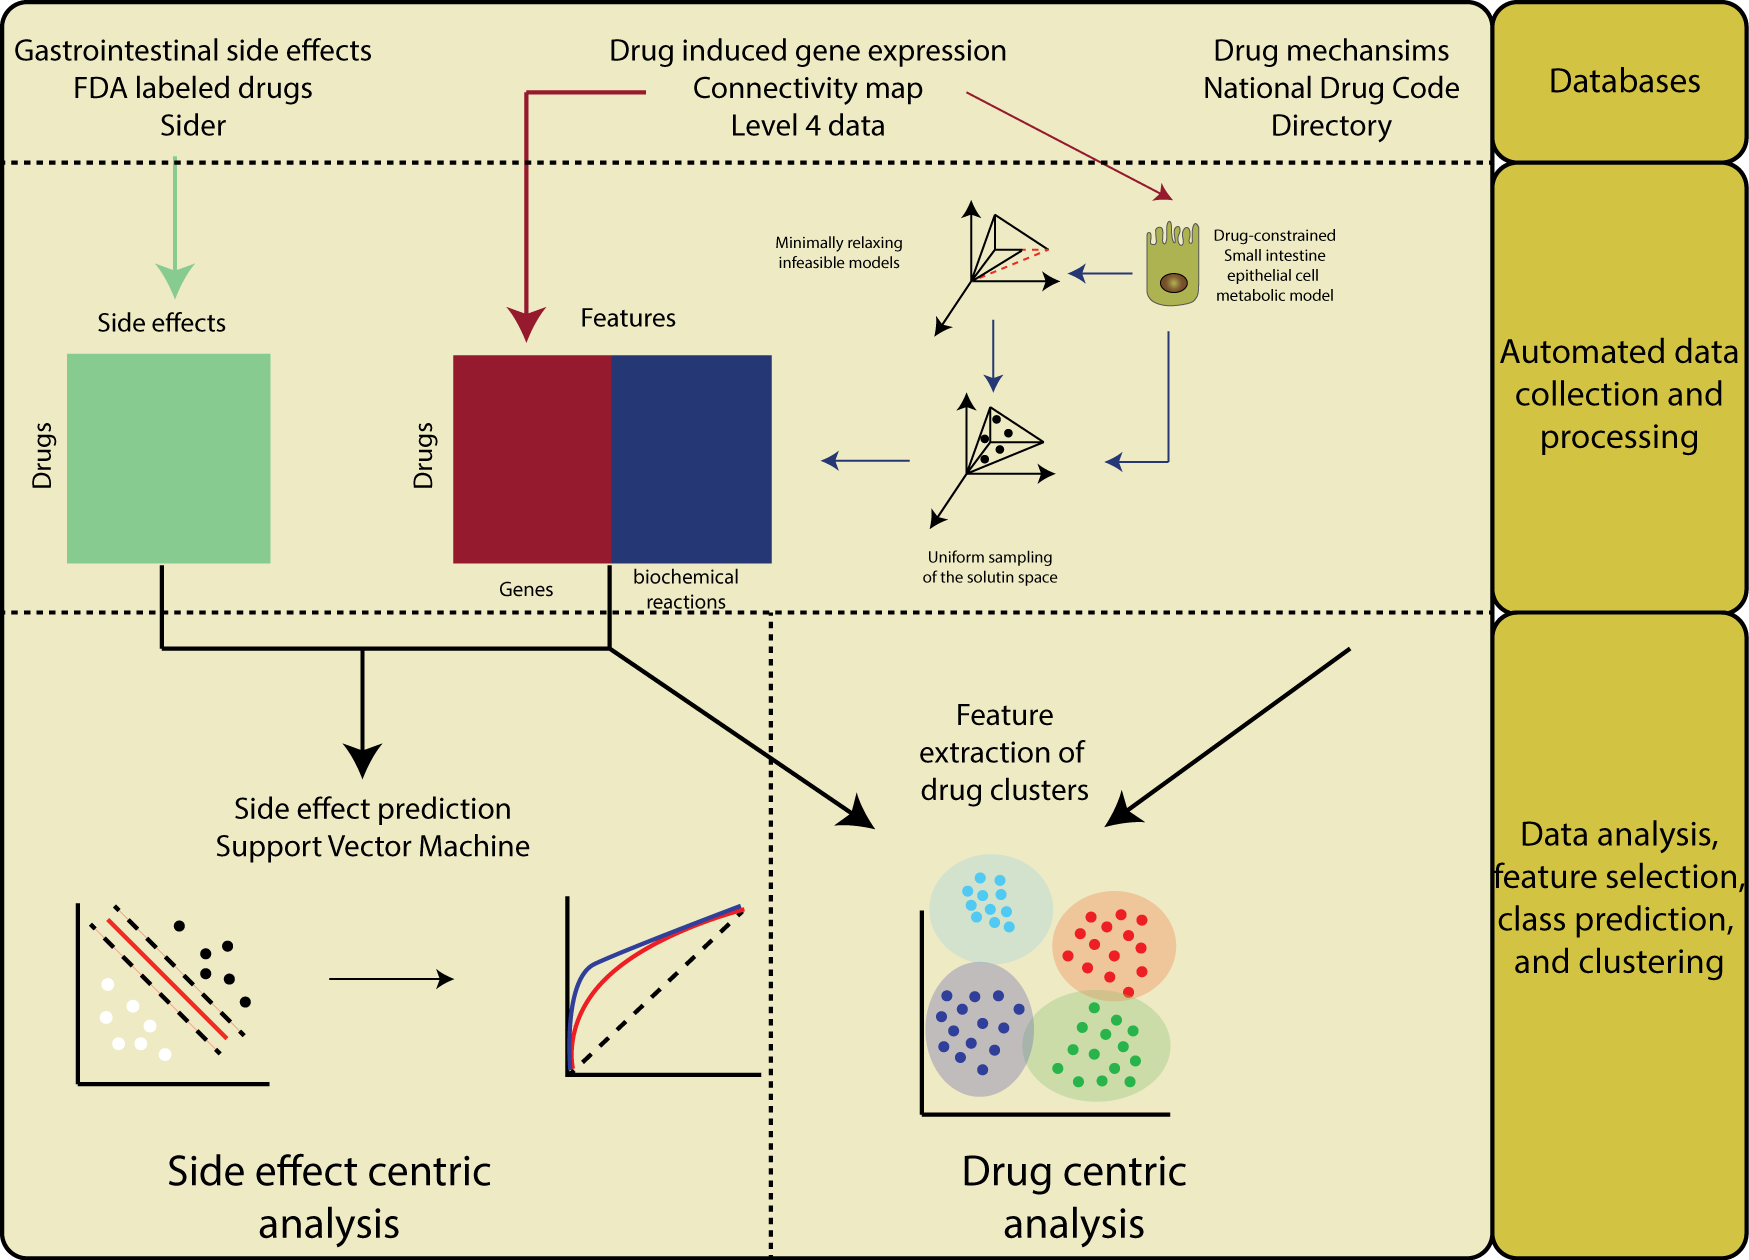
\includegraphics[width=\textwidth,height=\textheight,keepaspectratio]{sideEffects/Figure1.png}%Figure from images\Figure1.png
	\caption[Overview of the automatic data collection pipeline.]{Overview of the pipeline of data generation and analysis in this study. Drug induced gene expression were collected through the connectivity map API. The drug side effects occurrence was obtained from the SIDER database, and the drug mechanism and physiological effect was collected from the FDA National Drug Code Directory (NDCD). The drug-induced gene expression were subjected as constraints on a small intestine epithelial cell (sIEC) metabolic model to derive a context-specific model for each drug. After minimally resolving infeasible models, the uniform sampling of the solution space of the sIEC allowed to derive z-scores of metabolic fluxes in the treated and drug-free model. Combining the drug-induced gene expression with predicted differential metabolic fluxes in a single matrix allowed to train and cross-validate a multi-label support vector machine. Finally, the clustering of drugs based on their transcriptomic and metabolic profiles allowed to find hidden similarities beyond the indication based-classification.}
	\label{fig:seff1}
\end{figure}
In order to model drug effects on the gastrointestinal system, a manually-curated constraint-based model of the small intestinal epithelial cell (sIEC) \cite{sahoo2013predicting} was contextualized for each drug. The upper and lower bounds of every metabolic reaction were adjusted by the relative expression of the gene encoding the enzyme catalysing the reaction. The obtained context-specific drug-sIEC model was generated for every drug using the differential gene expression data obtained from the connectivity map \cite{subramanian2017next}. In models where the subjected constraints rendered the linear program infeasible, a set of reactions of minimal cardinality was relaxed by a minimal amplitude to obtain a feasible model. In order to assess the impact of drug constraints on metabolic models, the minimal and maximal metabolic flux per reaction was computed by FVA for each drug-constrained sIEC as suggested previously \cite{shaked2016metabolic}. Although, informing the classifier of the distribution of possible flux values per reaction rather than its bound could be of higher predictive capability. We sampled the drug-constrained solution space of each sIEC model and derived differential scores between the flux distribution per reaction of the drug-free sIEC and the drug-constrained sIEC. Following these steps, we obtained four features matrices: the differential gene expression of each drug obtained from the connectivity map, the FVA metabolism matrix obtained by the upper and lower bound of each reaction, the sampling metabolism matrix consisting of the differential score of flux value distribution per reaction, and the combined gene expression and sampled metabolism matrix which is a combination of the first and third matrices. The class matrix relating each drug to its side effects was obtained through parsing the SIDER database \cite{kuhn2015sider}. Further information about drug mechanisms, physiological effect, marketing date, and pharmacological class were obtained from the FDA NDCD database (Figure \ref{fig:seff1}).
\subsection{Combining measured gene expression and simulated gut wall metabolism predicts intestinal iatrogenic effects}
Drug induced gene expression provided strong features for side effect prediction, especially with side effect classes that have links to metabolism \cite{wang2016drug}. We used this finding to further improve the prediction of intestinal side effects through subjecting gene expression as constraints in the metabolic model of small intestine epithelial cell (sIEC), thereby contextualizing gut wall metabolism to derive the intestinal metabolic fingerprint of every drug. As previously observed \cite{wang2016drug}, gene expression alone was the support of most predictive features (Figure \ref{fig:seff2}-A). Metabolic reaction fluxes alone were less predictive as it takes into account the genes with metabolic activity in the sIEC (Figure \ref{fig:seff2}-A). Particularly, sampling the metabolic model allowed to improve the classification as it informs about the distribution of metabolic fluxes per reaction rather than the minimal and maximal bound of metabolic reactions alone as reported by FVA (Figure \ref{fig:seff2}-A). Combining gene expression and predicted metabolism gave the highest predictive rates in the multi-label SVM classifier as average of individual labels (Figure \ref{fig:seff2}-A), and in comparison to other classifiers (Figure \ref{fig:s1algo}).\\
Unspecific or likely non metabolic side effects such as gastrointestinal obstruction were among the least predictable with an area under the ROC curve of 0.67 using combined gene expression and sampled reaction fluxes. Side effects involving gut wall metabolism were highly predictable using combined features (Figure \ref{fig:seff3}, Table \ref{tbl:tbls3ch2}) such as intestinal carcinoma (0.96), ulcer (0.97), and toxicity (0.92). The merged intestinal side effect classifier using the individual binary classifiers could better predict (0.94) intestinal side effects based on combined gene expression and metabolism in comparison to gene expression (0.935)  or metabolism alone using FVA (0.92) and sampling (0.931) as shown by the micro-averaged ROC curve (Figure \ref{fig:seff2}-B). The most predictive metabolic reactions were enriched in the subsystems of sIEC and the most predictive genetic features were enriched in gene ontology biological processes database (both at p<0.001). The 10 most represented subsystems mainly involved transport in various locations (extracellular, exchange, mitochondrial, endoplasmic reticulum)  as well as catabolic and synthetic functionalities (Figure \ref{fig:seff2}-C). The gene ontology biological processes enriched groups involved mainly the regulation of transcription and apoptotic process (Figure \ref{fig:seff2}-D).  
\subsection{Drug  classification  using transcriptional and intestinal metabolic activity}
\begin{figure}[!ht]
\centering
	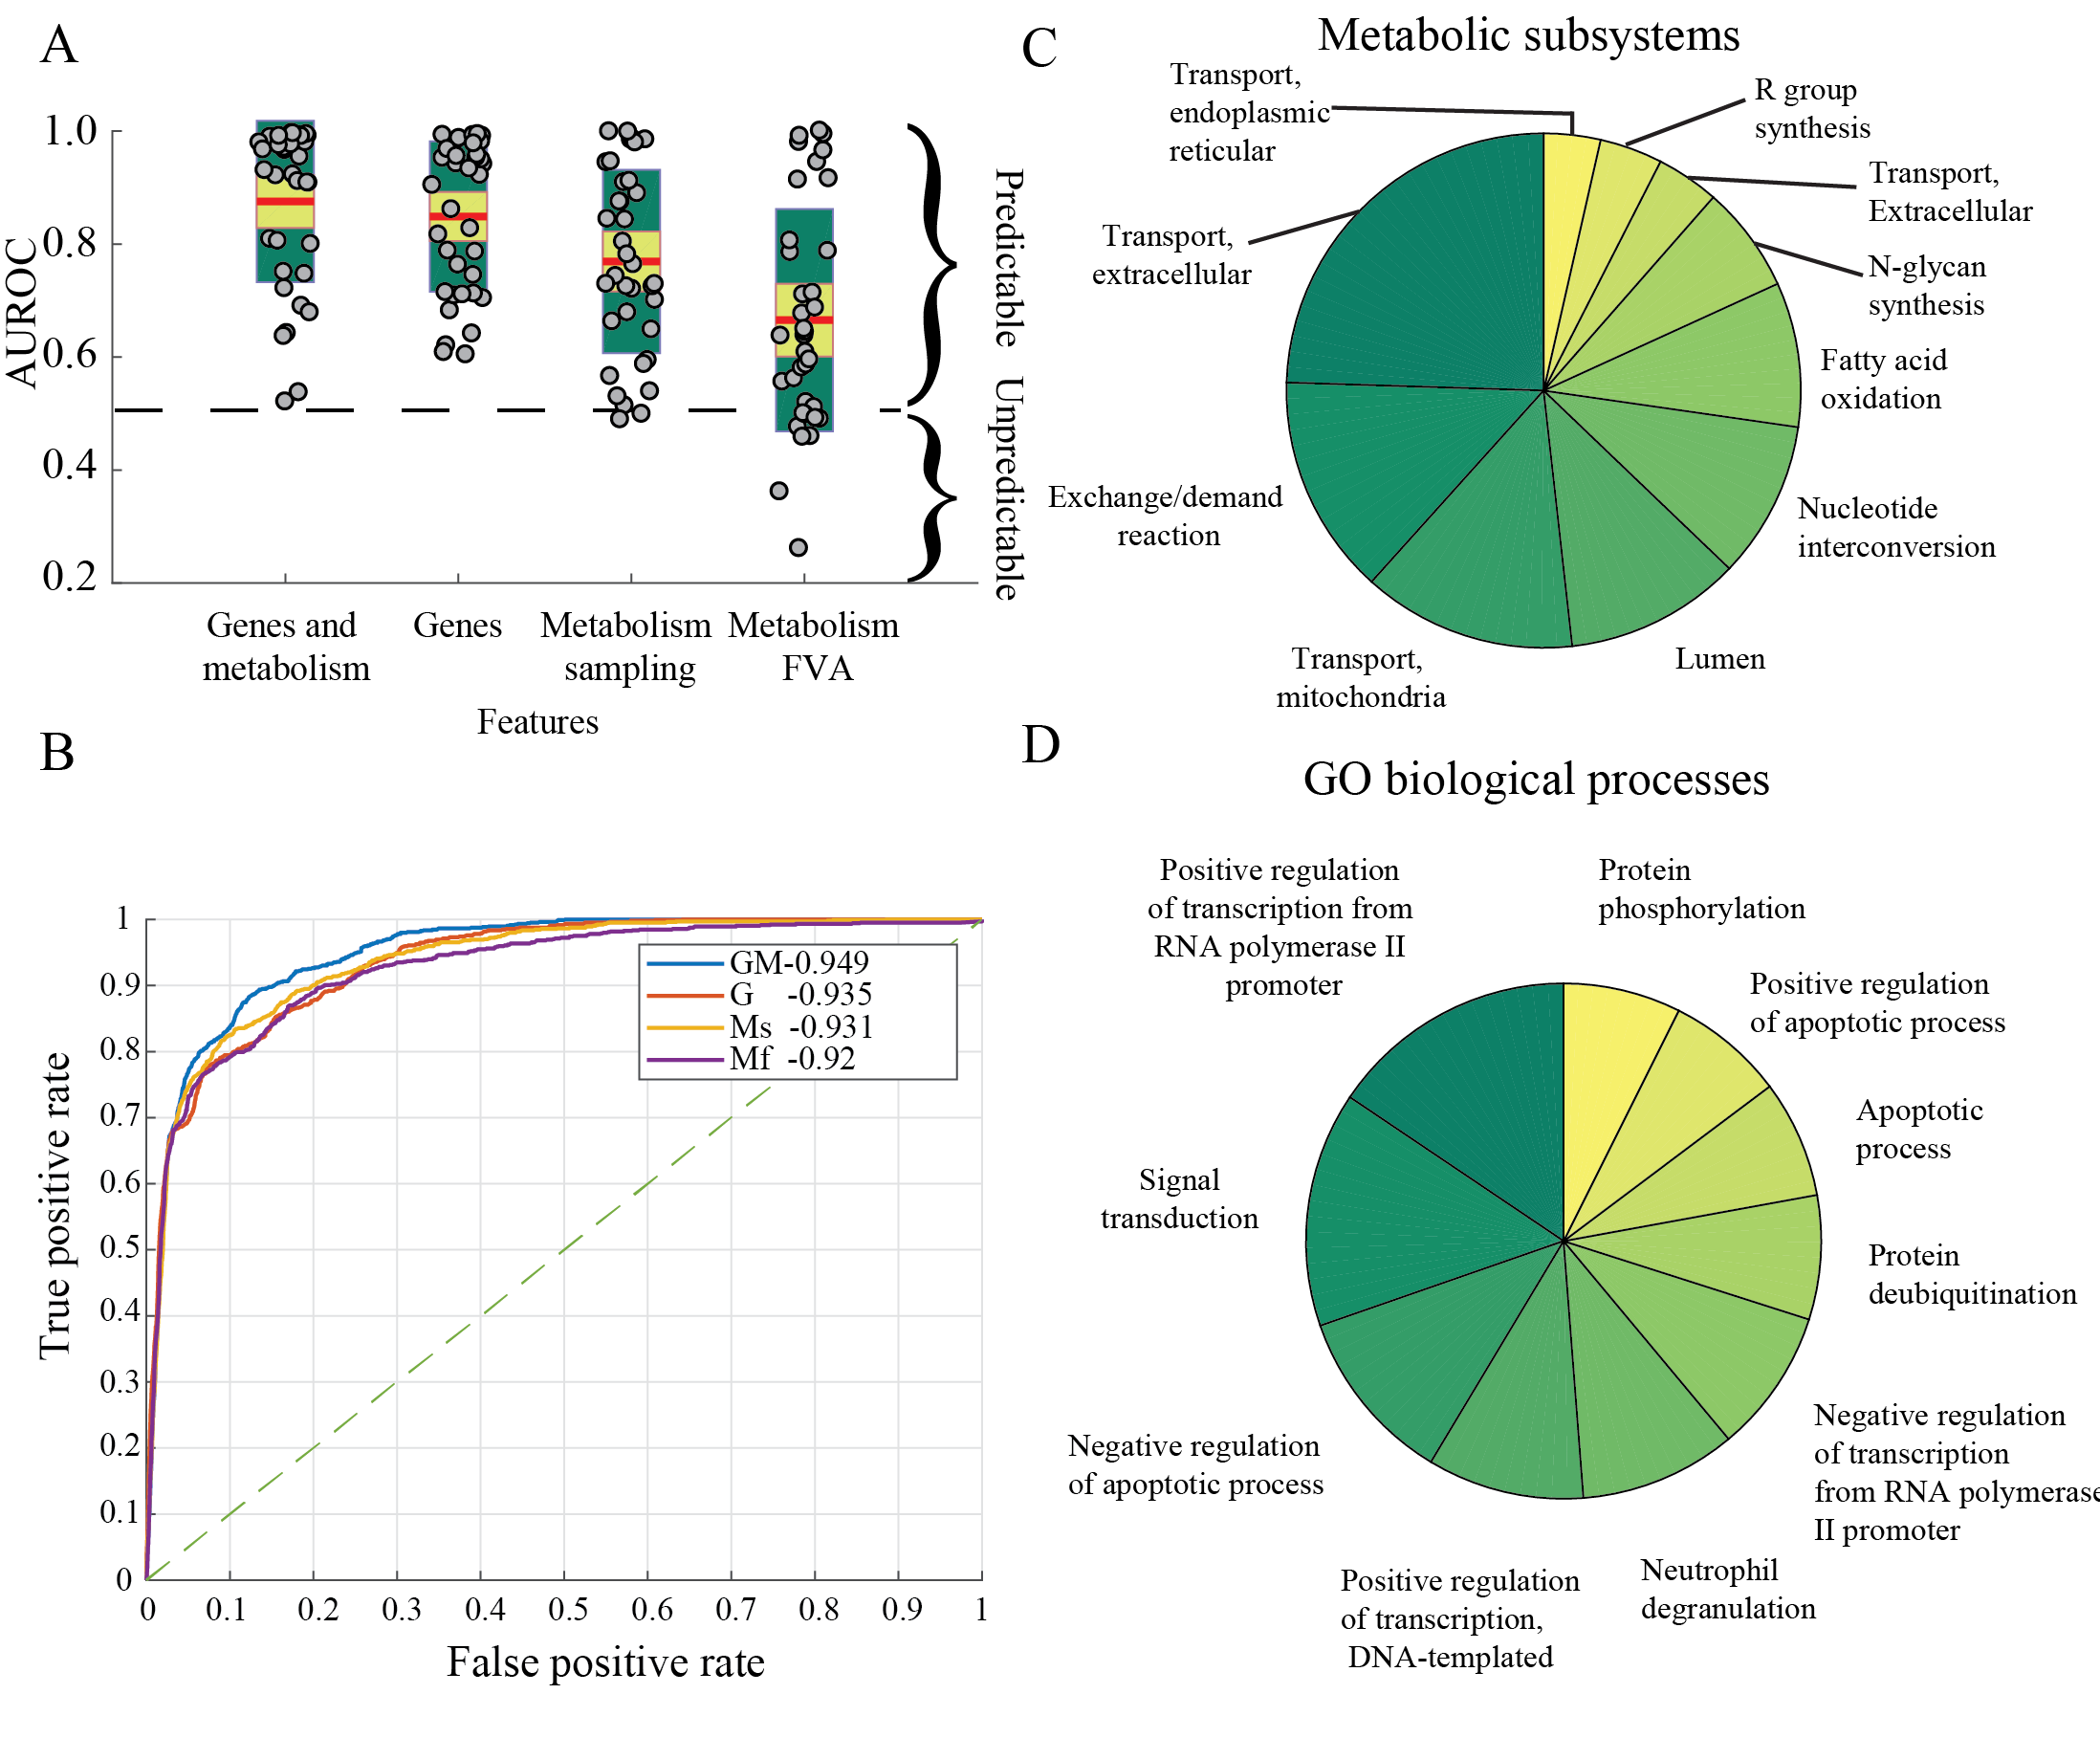
\includegraphics[width=\textwidth,height=\textheight,keepaspectratio]{sideEffects/Figure2.png}%Figure from images\Figure1.png
	\caption[Prediction performance of the multi-label SVM.]{Evaluation metrics for the multi-label support vector machine intestinal side effects classifier. A-Comparison of individual side effect classifier predictive capability as measured by the out-of-sample area under the ROC curve using genetic, metabolic, and combined genetic and metabolic features. B-ROC curve of the micro-averaged multi-label SVM classifier using genes, metabolism and combined genes and metabolism as features. C-Top 10 enriched metabolic subsystems and D-gene ontology biological process terms ranked by the number of metabolic and genetic representatives. G stands for genes, Ms for metabolism sampling, Mf for metabolism FVA, and GMs for genes and metabolism sampling.}
	\label{fig:seff2}
\end{figure}
\noindent The construction of the drug feature matrix consisting of gene and metabolic reaction vectors per drug allowed the use of clustering techniques to classify drugs in the gene and metabolism space. Using the community detection algorithm Jaccard-Louvain \cite{blondel2008fast}, we identified eight drug clusters based on their genetic and metabolic signature (Figure \ref{fig:seff4}-A). Each cluster had a stability and purity greater than 0.75 (Figure \ref{fig:s9seff}-D). In particular, transcriptional and intestinal metabolic activity were aligned with the identified clusters (Figure \ref{fig:seff4}-B). Interestingly, the identified clusters did not map on the FDA NDCD’s Established Pharmacological Class (EPC) (Figure \ref{fig:s9seff}-A) suggesting that classical indication-based classification could overlook genetic and molecular aspects of small molecules' pharmacodynamics. Most small molecules had a low genetic and  metabolic fingerprint as reported previously \cite{kuleshov2016enrichr} and targeted mainly the various transport subsystems (Figure \ref{fig:s9seff}-C) of the enterocyte, which is the main function of the gut wall. Cluster one and eight involved a high number of genes and metabolic reactions mainly due to cytotoxic drugs which was also reflected on the FDA NDCD’s Physiological Effect (PE) (Figure \ref{fig:seff4}-C) by the presence of terms linked to inflammation and immunity. Additionally, cluster eight and one were linked to malignant side effects (Figure \ref{fig:s9seff}-A).\\
Cluster seven had a high number of active fluxes in the small intestine epithelial cell. Interestingly, a number of terms linked to the central nervous systems were found, which hints to potential gut-brain shared molecular processes, probably linked to the similar composition of the blood brain barrier and the gut wall transporters \cite{banks2008blood}. In addition to cluster seven, cluster two had a low transcriptomic and a high metabolic profile. The EPCs linked to these clusters were mostly compounds whose action is mediated through metabolic, e.g., xanthine oxidase, or signalling, e.g., PPAR$\alpha$ molecule binding (Figure \ref{fig:seff4}-D). Ubiquitous targets, e.g., cyclooxygenase and histamine receptors would consequentially induce pronounced metabolic effects.\\
On the high transcription and high metabolism profile represented by cluster one and eight (Figure \ref{fig:seff4}-E), the presence of molecules acting on the central nervous systems by their FDA NDCD’s Mechanism of Action (MoA) confirms links between the gut and brain metabolism. Additionally, since cluster one and eight encompassed anticancer drugs as previously observed, this finding further supports ongoing repurposing trials of antidepressants in cancer therapy \cite{jahchan2013drug}. 
Moreover, neurokinin-1 antagonists, a class of drugs prescribed for the suppression of cytotoxic drug-induced emesis, and 5-lipoxygenase inhibitors, indicated for inflammatory bowel disease, had a high genetic and metabolic profile indicating potential links between gut symptomatology and genome-wide transcriptional and metabolic modulation. 
%Expectedly, antibiotics were among cluster one and cluster eight. 
%Noteworthy was the presence of several compounds associated to the cardiovascular system. 
We further enriched the top differentially enriched genes in each cluster in the KEGG \cite{chen2013enrichr,kanehisa2017kegg} database (Figure \ref{fig:seff4}-E) and selected the terms pertaining to gastrointestinal physiology. Epithelial cell signalling in \textit{H. pylori} infection was linked to cluster seven which had low transcriptomic and high metabolic profile suggesting metabolism-modulated signalling through kinases following the infection. \textit{E.coli} infection term belonged to the same cluster which suggests that both pathogens might involve the same kinase but also that similar treatment might overcome both infections. Phenotypes involving rather signalling mechanisms than metabolism e.g., \textit{Vibrio cholerae} infection belonged to cluster six that had low intestinal metabolic fingerprint. \\
Taken together, the multi-layer biology of drug effects allowed to accurately predict iatrogenic gastrointestinal effects using an SVM classifier. The clustering of drugs based on their metabolic and genetic signature has the potential to unravel potential similarities in the mechanism of action of compounds in relation to their physiological effects.
\begin{figure}[!htp]
\centering
	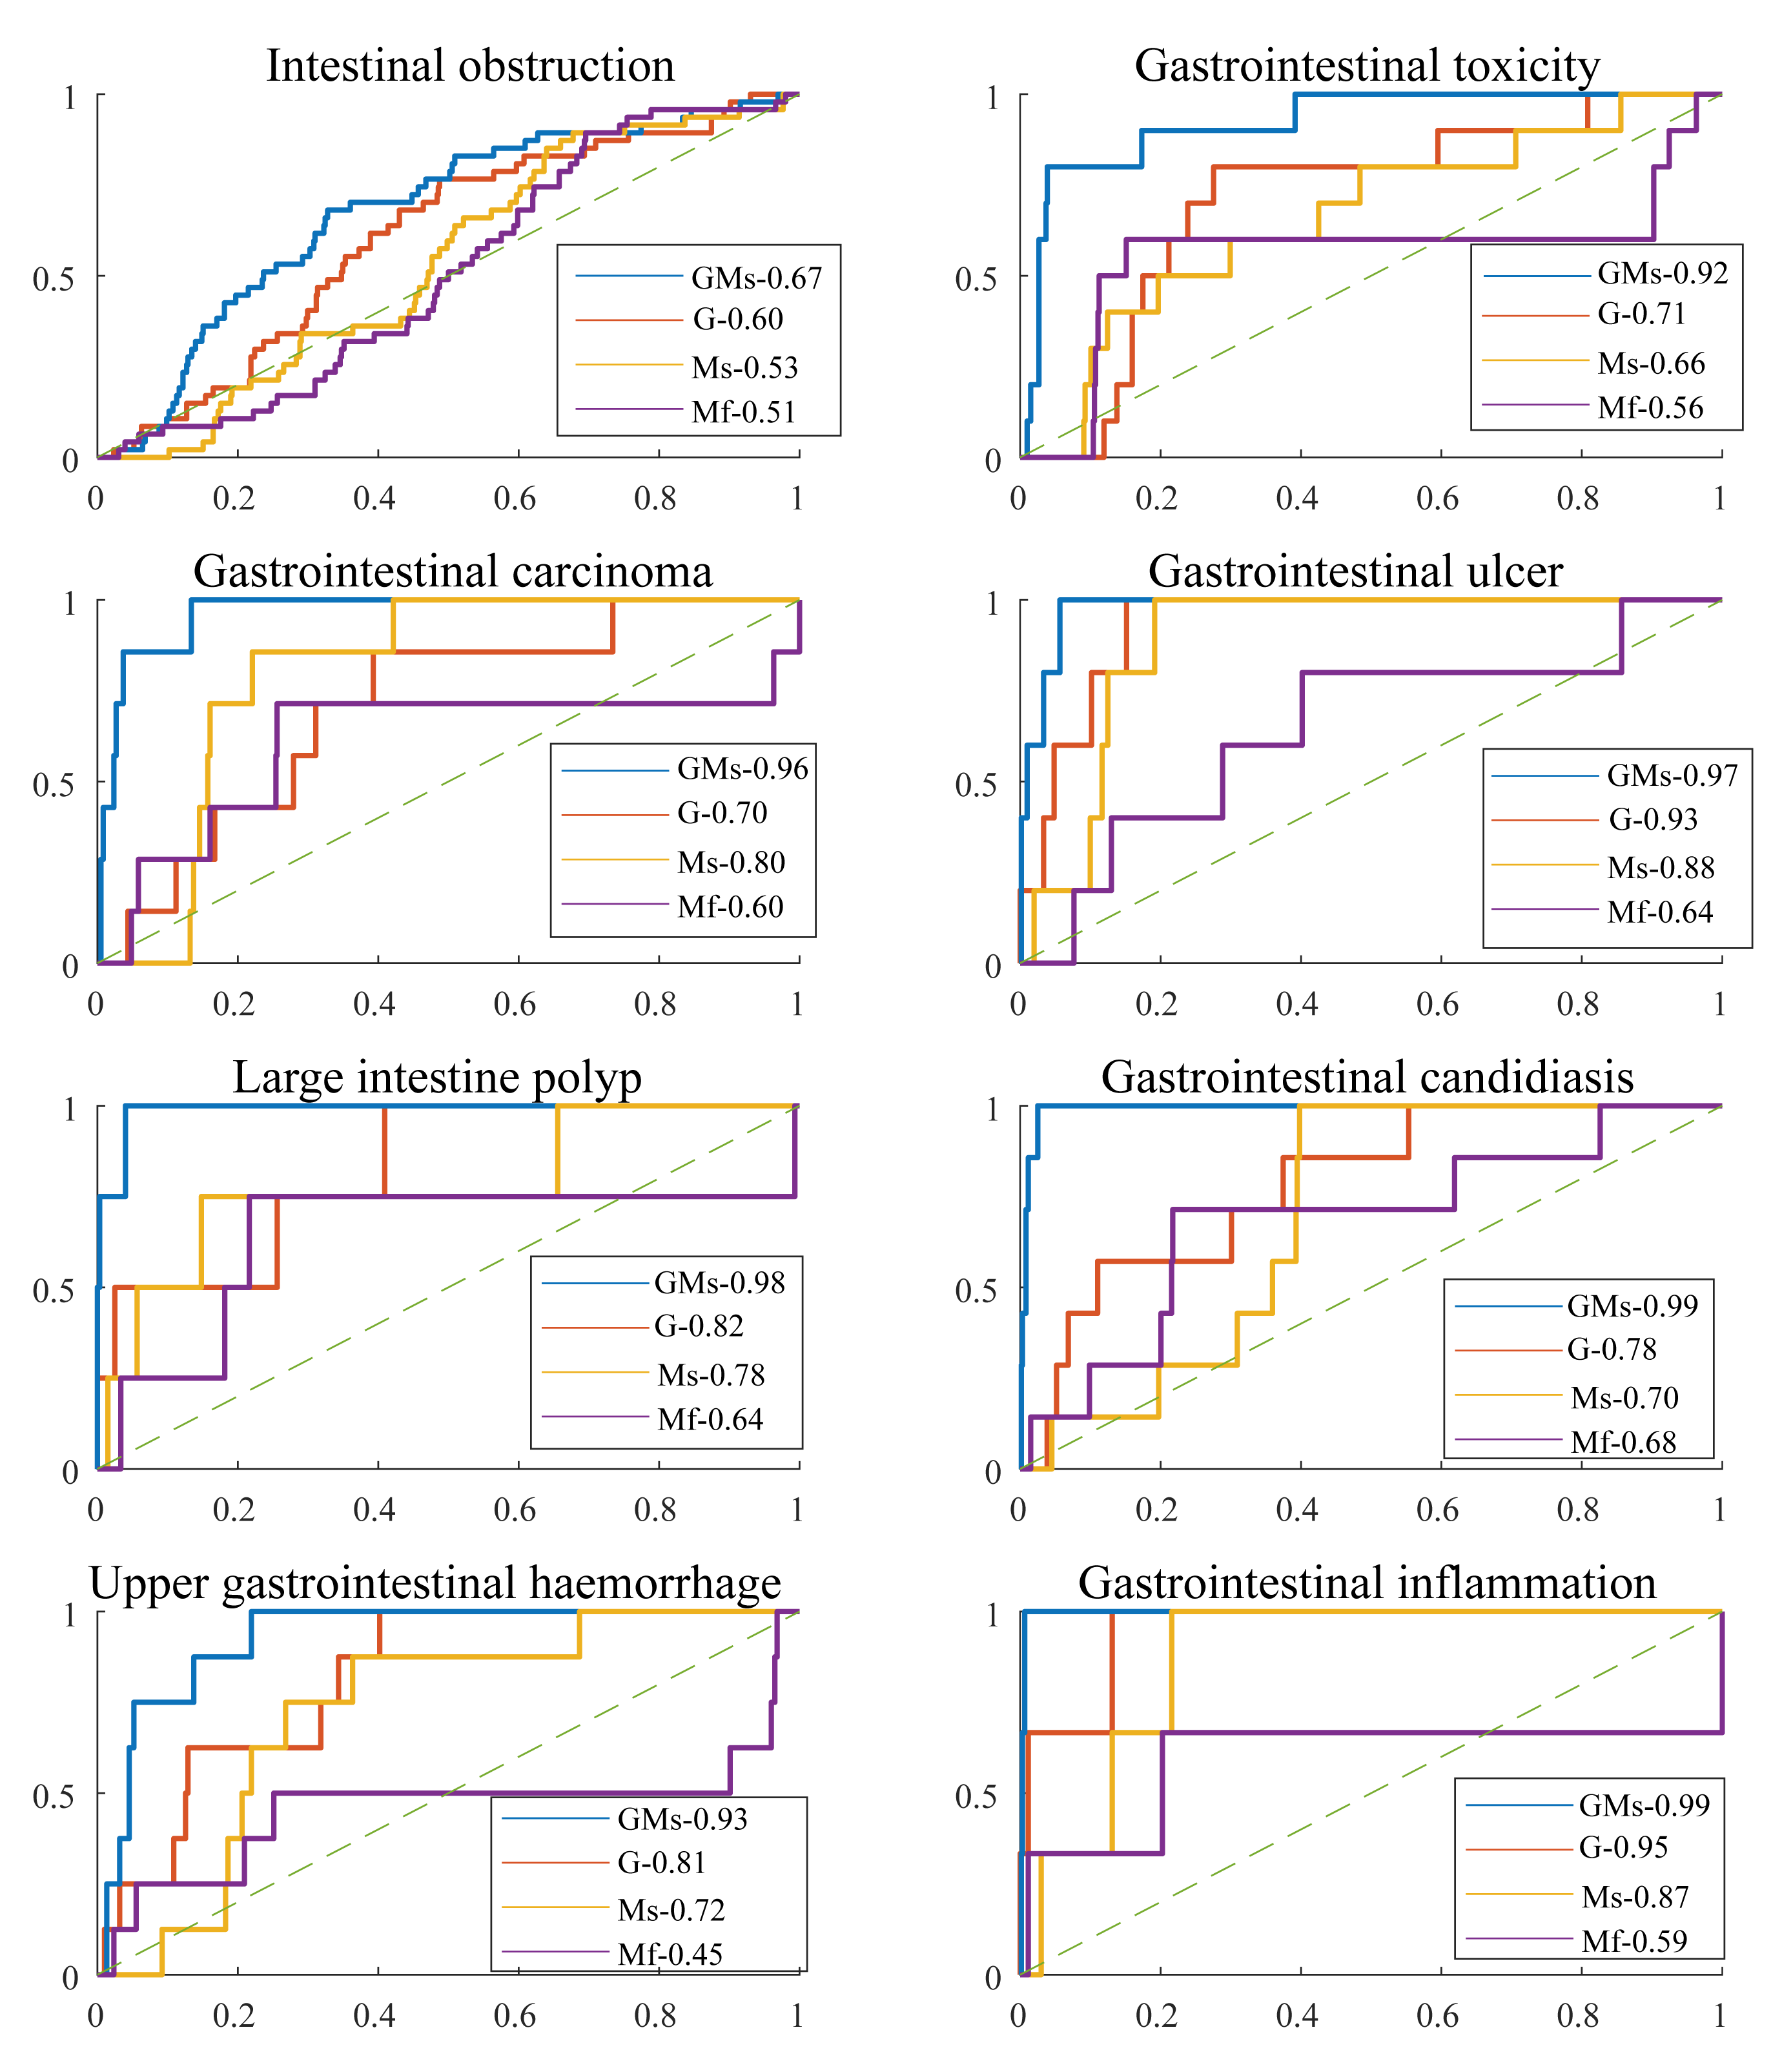
\includegraphics[width=\textwidth,height=\textheight,keepaspectratio]{sideEffects/Figure3.png}%Figure from images\Figure1.png
	\caption[Prediction of individual side effect labels.]{(Continued on the following page.)}
	\label{fig:seff3}
\end{figure}
\begin{figure}[t]
  \contcaption{Out-of-sample ROC curve for intestinal obstruction, gastrointestinal toxicity, carcinoma, ulcer, polyp, candidasis, hemorrhage, and inflammation. The features used for comparison were the sampled flux values in metabolic models, the minimal and maximal flux values per reaction as reported by FVA, gene expression reported in the connectivity map, and the combined gene expression and sampled reaction flux value. The comparison was performed using the area under the ROC curve. G stands for genes, Ms for metabolism sampling, Mf for metabolism FVA, and GMs for genes combined with metabolism sampling.}% Continued caption
\end{figure}
\section{Discussion}
The prediction of side effects using only \textit{in vitro} data of small molecules is a requisite of safe first-in-human trials and low attrition rates in the clinical phases.  The connectivity map of drug signatures \cite{subramanian2017next} provided a large set of gene expression profiles corresponding to small molecules perturbagens. Therefore, we modelled the metabolism of gut wall under drug-induced perturbation to predict iatrogenic effects using an SVM classifier. Sampling of the metabolic model provided better classification results than FVA bounds as features. Moreover, combining gene expression with modelling captured both metabolic and non-metabolic effects in relation to side effect development. Finally, classifying compounds with respect to their metabolic and transcriptomic fingerprint suggested drug repurposing strategies that could provide new therapeutic alternatives.
\subsection{Model generation and parameter selection}
\begin{figure}[!htp]
\centering
	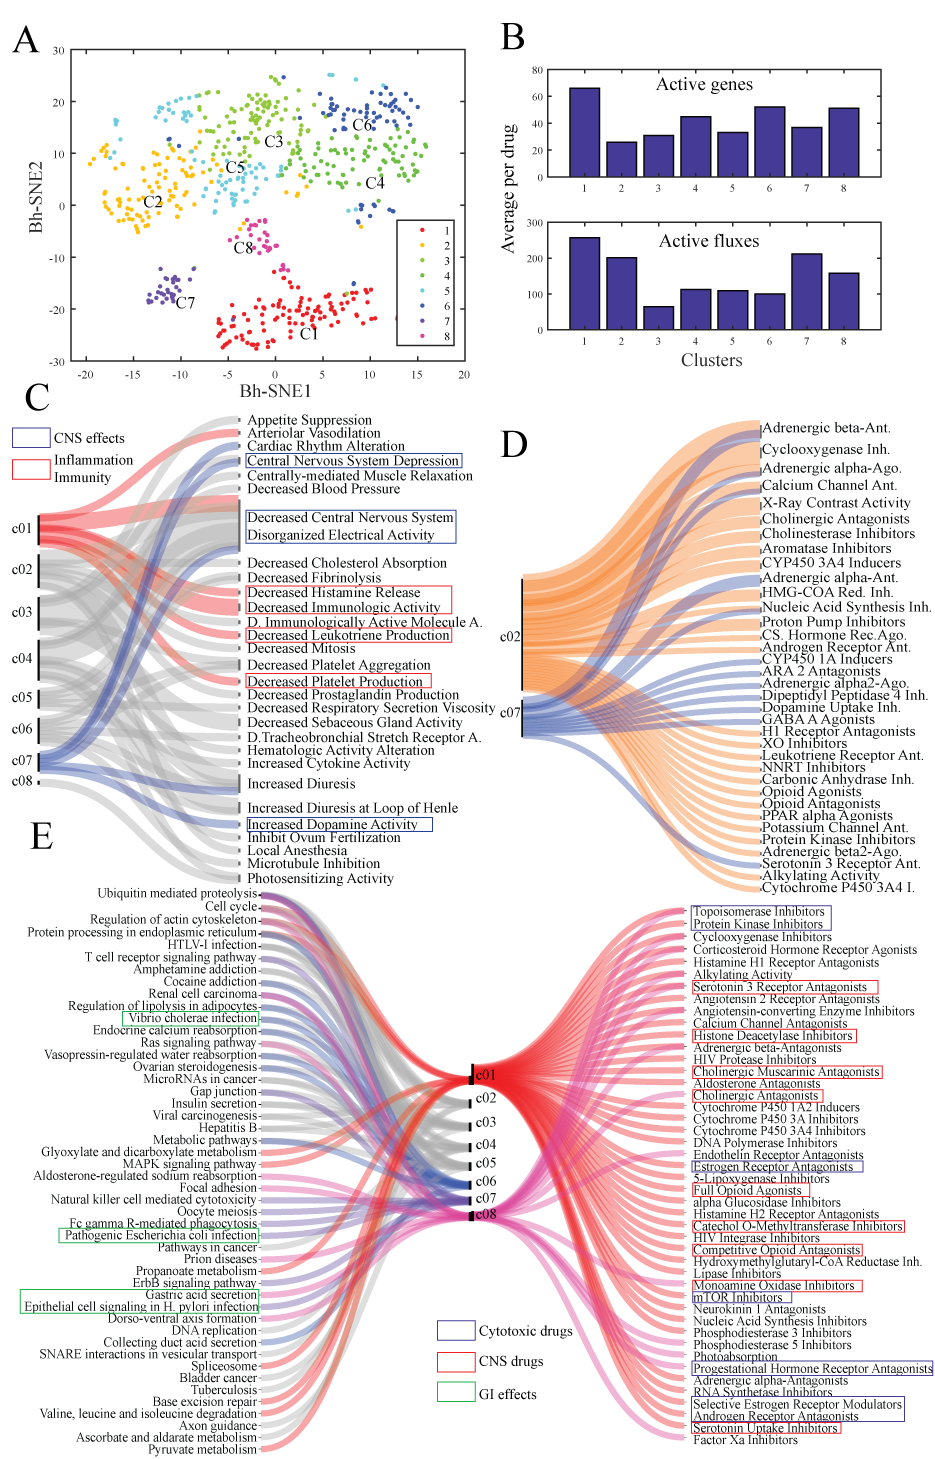
\includegraphics[width=\textwidth,height=\textheight,keepaspectratio]{sideEffects/Figure4.png}%Figure from images\Figure1.png
	\caption[Drug community detection.]{(Continued on the following page.)}
	\label{fig:seff4}
\end{figure}
\begin{figure}[t]
  \contcaption{Drug community identification based on measured transcriptional and simulated gut wall metabolic profile. A-Visualisation of the eight validated drug clusters through Barnes-Hut Stochastic Neighbourhood Embedding (Bh-SNE) plot. B-Transcriptional and gut metabolic activity of the identified clusters showed different levels of drug specificity per cluster. C-Bipartite graph of drug clusters and FDA NDCD's physiological effect (PE). D-Bipartite graph of drug clusters and FDA NDCD’s established physiological class (EPC). E-Graph linking drug clusters to FDA NDCD’s mechanism of action (MoA) and KEGG enriched pathways of the gene pertaining to each cluster. The diagram was done using Rawgraphs \cite{Mauri:2017:RVP:3125571.3125585}.}% Continued caption
\end{figure}
The connectivity map \cite{subramanian2017next} provided a large-scale resource of small molecule transcriptomic signature and enabled the genome-wide assessment of drug off-target effects, thereby expanding pharmacology beyond the study of the drug primary target alone. The integration of drug-induced gene expression with generic metabolic models of human metabolism allowed to identify key disrupted metabolic functions \cite{zielinski2015pharmacogenomic} resulting from adverse reactions. Similarly, the integration of known target effects of drugs as identified from DrugBank \cite{wishart2017drugbank}, and using flux bounds obtained by FVA as features to predict side effects \cite{shaked2016metabolic} allowed to accurately predict several classes of side effects. Although, this approach remains limited to drugs with inhibitory effects on metabolic targets, and \textit{a fortiori} of known targets. In our approach, the integration of drug-induced gene expression with metabolic networks allowed to circumvent the inhibitory target limitation \cite{sahoo2015modeling} and allowed most importantly to model the drug off-target effects which were suggested to be the main driver of side effects. We showed that informing the classifier with the distribution of metabolic fluxes per reaction using sampling rather than providing the bounds of the reaction using flux variability analysis increased the predictive power of the classifier (Figure \ref{fig:seff2}-A,B). Additionally, restricting the prediction to a set of organ-specific side effects using a manually curated tissue-specific metabolic model captured local metabolism in relation to the emergence of organ-specific adverse reactions.\\
Improving the prediction of occurrence of side effects relies greatly on the quality and completeness of the dataset used. It is highly likely that weighting the variables by the side effects frequency per drug can improve the predictions and leverage the prediction of rare side effects. Nevertheless, only 46\% of side effects had frequency information associated whose inclusion did not improve the prediction accuracy (Figure \ref{fig:s6seff}). The missing information could be potentially filled by either manual expert curation or crossing databases. Moreover, the physiological effect and mechanism of action in the FDA NDCD were missing for a number of drugs as well. 
Additionally, the chronopharmacology of drug action is also of paramount importance in detecting the emergence of side effects. The connectivity map provides a number of experiments at several time interval that we did not exploit in our analysis as not all drug-induced gene expression were measured for different time points. Such data can take the predictions from looking at snapshots of transcription and metabolism to dynamical models linking the emergence of  side effects to time-dependant processes.
\subsection{Sampling the metabolic model of the gut wall achieved the highest prediction accuracy}
Conceptually, drug-induced gene expression could play a major role in the genesis of adverse reactions. Particularly, it was shown to be predictive towards side effects classification, especially when combined with other drug features such as chemical structure and cell morphology after treatment \cite{wang2016drug}. The combination of gastrointestinal local metabolism constrained by metabolic gene expression and the differential expression of non-metabolic genes allowed to achieve the most accurate prediction of gastrointestinal side effects (Figure \ref{fig:seff2}-A,B). The combination of multiple layers of biology consisting of transcriptomic and predicted metabolic features was key in capturing drug-induced perturbations related to side effects. Furthermore, the approach can be scaled to several tissues to include all the label of side effects using semi-automatic and manually curated models of human metabolism \cite{schultz2016reconstruction}. Remarkably, sampling metabolic models alone achieved a good accuracy taking into account that only the metabolic subset of genes from the connectivity map was modelled. Therefore, we suggest that a reduced set of \textit{in vitro} experiments to measure the differential expression of metabolic genes would give an invaluable insight into the emergence of adverse reactions of a new chemical entity in the preclinical phase which can guide the rational design of first-in-human trials. Furthermore, the emergence of whole-cell models \cite{karr2012whole,szigeti2017blueprint} that integrate metabolism alongside several physiological functions would allow the mapping of non-metabolic genes onto computational models of the cell to capture the cell-wide disruption of physiological processes that lead to the emergence of side effects. With the generated combined gene and gut wall metabolism matrix in hand, we classified the small molecules with respect to their signatures to highlight their common features.
\subsection{Drug reclassification beyond the chemical class}
Drugs are often classified with respect to their pharmacological indication and their chemical family. The many examples of marketed drug repurposed for new indications \cite{li2015survey} shows that a small molecule can have rather many effects. Drug repurposing have gained great interest in the recent years, as it allows to greatly decrease the drug development process using compounds whose safety is well documented.  
In order to find common properties of drugs, we identified clusters of compounds that share similar genetic and metabolic signatures in the gut wall. Interestingly, compounds that involved a high number of metabolic reactions with a high amplitude of variation included CNS drugs like serotonin antagonists indicated for psychotic episodes that were later suggested to treat chemotherapy-induced emesis. Moreover, those compounds belonged to the same cluster with neurokinin inhibitors that are primarily indicated for the prevention of emesis as well. Serotonin antagonists are also indicated to treat the inflammatory bowel syndrome, which further showed the similarity between the blood brain barrier and the gut wall metabolism and gene expression. Furthermore, anticancer drugs and the drugs that treat their side effects, the anti-emesis drugs, clustered together in the high transcriptomic, high metabolic activity cluster, further supporting the idea that reversing the molecular fingerprint of a compound can reverse its effects. Particularly, reversing the fingerprint of the compound locally, in the gut wall, would be a potential strategy to reverse gastrointestinal side effects of drugs through the administration of co-drugs, while preserving its main activity in the target tissue.\\
Furthermore, the clusters of drugs that we identified in our analysis did not match FDA marketing date (Figure \ref{fig:s9seff}-B). Despite the emergence of the key-lock paradigm \cite{medina2013shifting} in drug development using molecular dynamics and docking experiments in early 1990s that decreased the number of drugs interacting with a high number of targets, colloquially  called 'dirty drugs', there are still opportunities for further enhancement in the design of precise therapies. \\
We developed and employed a multi-label support vector machine on genetic and metabolic fingerprint of marketed small molecule compounds to accurately predict the occurrence of gastrointestinal side effects. The drug features allowed to classify drugs based on their metabolic and genetic profile, which is a promising avenue for drug repurposing to revert side effects and unravel new indications. The development of large scale, publicly available, compound resources combined with complex mathematical models of cellular biology provides a new way of providing patients with safer and more effective therapies.
\subsection*{Acknowledgements}
The authors would like to acknowledge Dr. Peter Banda at the Luxembourg Centre for Systems Biomedicine (LCSB) for the helpful discussions and the important suggestions on the work as well as the Molecular Systems Physiology lab members at the LCSB for insightful comments on the manuscript and in particular Alberto Noronha for technical assistance. 
%Path to chapter

\chapter{Model-based dietary optimization for late-stage, levodopa-treated, Parkinson's disease patients.}
\label{ch:chapter3}
\chaptermark{Levodopa-diet interaction}%Short description for page header
{\setstretch{1.0} Guebila, MB., Thiele, I. (2016). Model-based dietary optimization for late-stage, levodopa-treated, Parkinson's disease patients. \textit{NPJ Syst Biol Appl}. \href{https://www.nature.com/articles/npjsba201613}{DOI: 10.1038/npjsba.2016.13.}  \par}%Paper reference, note, other. Can remove. Single line space.
\section*{Abstract}
{\setstretch{1.0}  
Levodopa has been the gold standard for Parkinson’s disease treatment for more than 40 years. Its bioavailability is hindered by dietary amino acids, leading to fluctuations in the motor response particularly in late-stage (stage 3 and 4 on Hoehn and Yahr scale) patients. The routine dietary intervention consists of low-protein (< 0.8 g/kg) diets or the redistribution of daily protein allowance to the last meal. Computational modeling was used to examine the fluctuation of gastrointestinal levodopa absorption under consideration of the diet by (i) identifying the group of patients that could benefit from dietary interventions, (ii) comparing existing diet recommendations for their impact on levodopa bioavailability, and (iii) suggesting a mechanism-based dietary intervention.
We developed a multiscale computational model consisting of an ODE-based ACAT model and metabolic genome-scale sIEC model. We used this model to investigate complex spatiotemporal relationship between dietary amino acids and levodopa absorption. Our model predicted an improvement in bioavailability, as reflected by blood concentrations of levodopa with protein redistribution diet by 34\% compared with a low-protein diet and by 11\% compared with the ante cibum (a.c.) administration. A systematic analysis of the effect of different amino acids in the diet suggested that a serine-rich diet could improve the bioavailability by 22\% compared with the a.c. administration. Optimizing dietary recommendations in quantity, composition, and intake time holds the promise to improve levodopa efficiency and patient’s quality of life based on mechanistic models of gut physiology.
\par}%single line space

\newpage
\section{Introduction}
The gut wall is the first physiological barrier that encounters nutrients and xenobiotics absorbed orally \cite{lennernas1998human}, where food–drug interactions take place. These interactions are complex, as in the case of levodopa absorption and a protein-rich diet. Levodopa is the gold standard treatment in Parkinson’s disease \cite{brooks2008optimizing} and has a similar chemical structure as cyclic amino acids\cite{eisenhofer1997substantial}. Supplementing Parkinson's disease patients with levodopa restores the dopamine levels in the brain and prevents motor symptoms \cite{fahn2015levodopa}. 
It shares the same transporters with amino acids in the gut, brain, and kidneys,leading to competition that decreases its entry to target sites\cite{nutt1984off}. Therefore, dietary recommendations are given to Parkinson's disease patients \cite{ishihara2005systematic} as levodopa bioavailability is influenced by diet\cite{contin2010pharmacokinetics}. Low-protein diet (LPD) limits protein intake to a minimal amount for every meal (< 0.8 g/kg of body weight). Another option is protein redistribution diet (PRD), where patients are recommended to take the daily protein allowance in the last meal. PRD has a better efficacy with lower off phenomena (e.g., akinesia) leading to improved life quality, especially at the latest stages of Parkinson's disease (3 and 4 on Hoehn and Yahr (HY) scale)\cite{cereda2010low}. The molecular mechanism of this improvement remains poorly understood. The recent identification of luminal and basolateral levodopa transporters in the human sIEC was a major step for a better evaluation of dietary recommendations. It has been shown that, in addition to luminal competition, the presence of amino acids in the basolateral side of enterocytes trans-stimulates the absorption of levodopa leading to a higher bioavailability of the drug \cite{camargo2014molecular}. Computational modeling could be used to further elucidate the role of diet and levodopa absorption and to provide a basis for rational design of dietary recommendations. Such modeling should ideally (i) describe the levodopa kinetics in the gastrointestinal tract, as well as the other organs and (ii) consider sIEC-mediated uptake of levodopa and dietary amino acids.For the first aspect, PBPK modeling is an ideal computational approach because it describes with a set of ordinary differential equations cellular, tissue, and whole-body distribution of drugs. In particular, whole-body generic PBPK models have been described in the literature and used to investigate the effects of xenobiotics and mechanistically predict tissue concentrations of drugs \cite{jones2013basic}.
Moreover, organ and process-specific PBPK models have been developed, such as the ACAT model, for which in vitro parameters were used to estimate gastrointestinal absorption of drugs in human along seven small intestinal segments \cite{agoram2001predicting}. An advantage of the PBPK modeling is that it captures the dynamics of the modeled system. However, it requires the availability or fitting of many parameters, which may not be always easy to be obtained and thereby limits the size and resolution of the described system. In contrast, the COBRA approach assumes the modeled biological system to be at a steady state, thereby allowing the description of large systems, such as cells and organs, at the molecular level, while not requiring complete knowledge about the model parameters\cite{o2015using}. COBRA models are assembled based on genome annotations and biochemical data \cite{thiele2010protocol} and subjected to physio-chemical, genetic, thermodynamic, and biological constraints\cite{beard2002energy}. Recently, a genome-scale model of the enterocyte-specific metabolism (‘sIEC model’) has been published, describing known metabolic transformations and transport activities in sIECs\cite{sahoo2013predicting}. This model has been constructed on the basis of global human metabolic reconstruction \cite{duarte2007global} which has been also recently extended for more refined metabolic content\cite{thiele2013community}\cite{sahoo2014membrane}, as well as for a drug module\cite{sahoo2015modeling}. In this study, we (i) develop a combined multiscale PBPK–COBRA model and (ii) use it to investigate the complex spatiotemporal relationship between amino acids and levodopa kinetics and its impact on Parkinson's disease patients.

\section{Methods}
To generate the multiscale gastrointestinal model, we (i) expanded the
whole-body generic PBPK model\cite{peters2008evaluation} by the ACAT model\cite{agoram2001predicting}, (ii) added levodopa transport reactions to the sIEC model \cite{camargo2014molecular}, and (iii) coupled both models with respect to a specific time step.
\subsection{Whole-body PBPK modeling and system identification}
The ACAT model\cite{agoram2001predicting} and the whole-body generic PBPK \cite{jones2013basic} (Figure \ref{fig:multiscale},Figure {fig:s1levo}-A) model were implemented and combined in Matlab (2014b release, MathWorks, Natick, MA, USA). Details on the models and their integration can be found in the supplementary section dynamical modeling of levodopa (Text \ref{levo:sp1}). The whole-body generic PBPK model with ACAT component consisted of 42 ordinary differential equations and 243 parameters. In the following, we will refer to this ACAT-expanded whole-body generic model as WB-ACAT model.
The kinetic parameters of levodopa (Table \ref{tbl:tbls1} and \ref{tbl:tbls2}) were identified through fitting of the WB-ACAT model on averaged data from 24 fasting healthy volunteers' plasma concentrations after oral (\textit{Per os}) administration of 200 mg of a standard formulation of levodopa and 50 mg of peripheral metabolism inhibitor (benserazide) \cite{keller2011comparative} ((Text \ref{levo:sp2}); Figure {fig:s1levo}-B). The goodness of fit was assessed through visual inspection (Figure {fig:s2levo}), the Kolmogorov–Smirnov test \cite{massey1951kolmogorov} with a resulting $P = 0.9994$, and the Pearson’s correlation coefficient with r = 0.99 (P < 0.0001).
The delay in the GER parameter induced by food was inferred by sequentially fitting data from a two-occasion study\cite{contin2010pharmacokinetics}: plasma levodopa concentrations in the fasted state and plasma levodopa concentrations after aproteic meal. For the first occasion (fasted), all model parameters were estimated except GER, which was set, as reported in the literature, for the fasting state (Table \ref{tbl:kineticparam}). For the second occasion (fed), all kinetic parameters were fixed and only GER was estimated. The sequential fitting approach was undertaken, as it allowed quantification of varying parameter between fed and fasted states.
The time-dependent parameter sensitivity analysis with respect to levodopa concentrations in plasma was computed as the result of the following non-normalized time-dependent derivative:\\
\begin{equation}
sensitivity =\frac{\partial y}{\partial x}
\end{equation}
where $x$ represents the vector of all WB-ACAT model parameters and $y$ represents the plasma concentrations of levodopa. Then, the absolute time integral for every parameter was computed for every parameter using \textit{trapz} function in Matlab.
\subsection{sIEC model}
To take into account the gut wall metabolism and transport, the sIEC stoichiometric model was used. The sIEC model contains a thorough collection of metabolic and transport pathways of amino acids, which provided non-intuitive metabolite utilization strategies in different conditions \cite{sahoo2013predicting}. To account for levodopa uptake and secretion by the transporters (EntrezGene ID: 11067-6591, 117247, 23428-6520), 36 levodopa reactions were added to the model, representing the specific stoichiometric coefficients for the transported co-metabolites accounting for competition and trans-stimulation (Text \ref{levo:sp3}) in the reported order of affinity \cite{verrey2000glycoprotein} as measured experimentally \cite{camargo2014molecular}. The resulting sIEC\_levodopa model, to which we will refer in the remainder as sIEC model, consisted of 433 metabolites, 1318 reactions, and 616 genes.
\subsection{Coupling algorithm}
The coupling between seven sIEC models and the WB-ACAT model (Figures 1 and 4) was achieved by performing dynamic flux balance analysis\cite{varma1994stoichiometric}, which computes uptake rates of each of the seven sIEC models using as constraints the outcome of the simulation of the WB-ACAT model, which were subsequently set as derivatives $\frac{dX}{dt}$ in the WB-ACAT model. We implemented this coupling with the static optimization approach (SOA) \cite{mahadevan2002dynamic}, which discretizes the simulation time into a defined number of steps and simulates sequentially the PBPK and COBRA model for every step \cite{mahadevan2002dynamic} (Figure \ref{fig:couplemethod}). The total simulation time of 18 h was divided into steps of 0.1 h, which represents a good compromise between the integration tolerance of the dynamical model, the simulation time, and the steady state assumption of the sIEC model with respect to the fast kinetics of levodopa in the blood following \textit{Per os} administration \cite{covert2008integrating}. SOA assumes steady state of the metabolic network in intervals of 0.1 h, the sIEC model will reach a different steady state depending on the changing constraints of levodopa between the different time intervals.
\section{Results}
\subsection{Modeling intestinal absorption of levodopa using a combined PBPK–COBRA model}
\begin{figure}[!htp]
\centering
	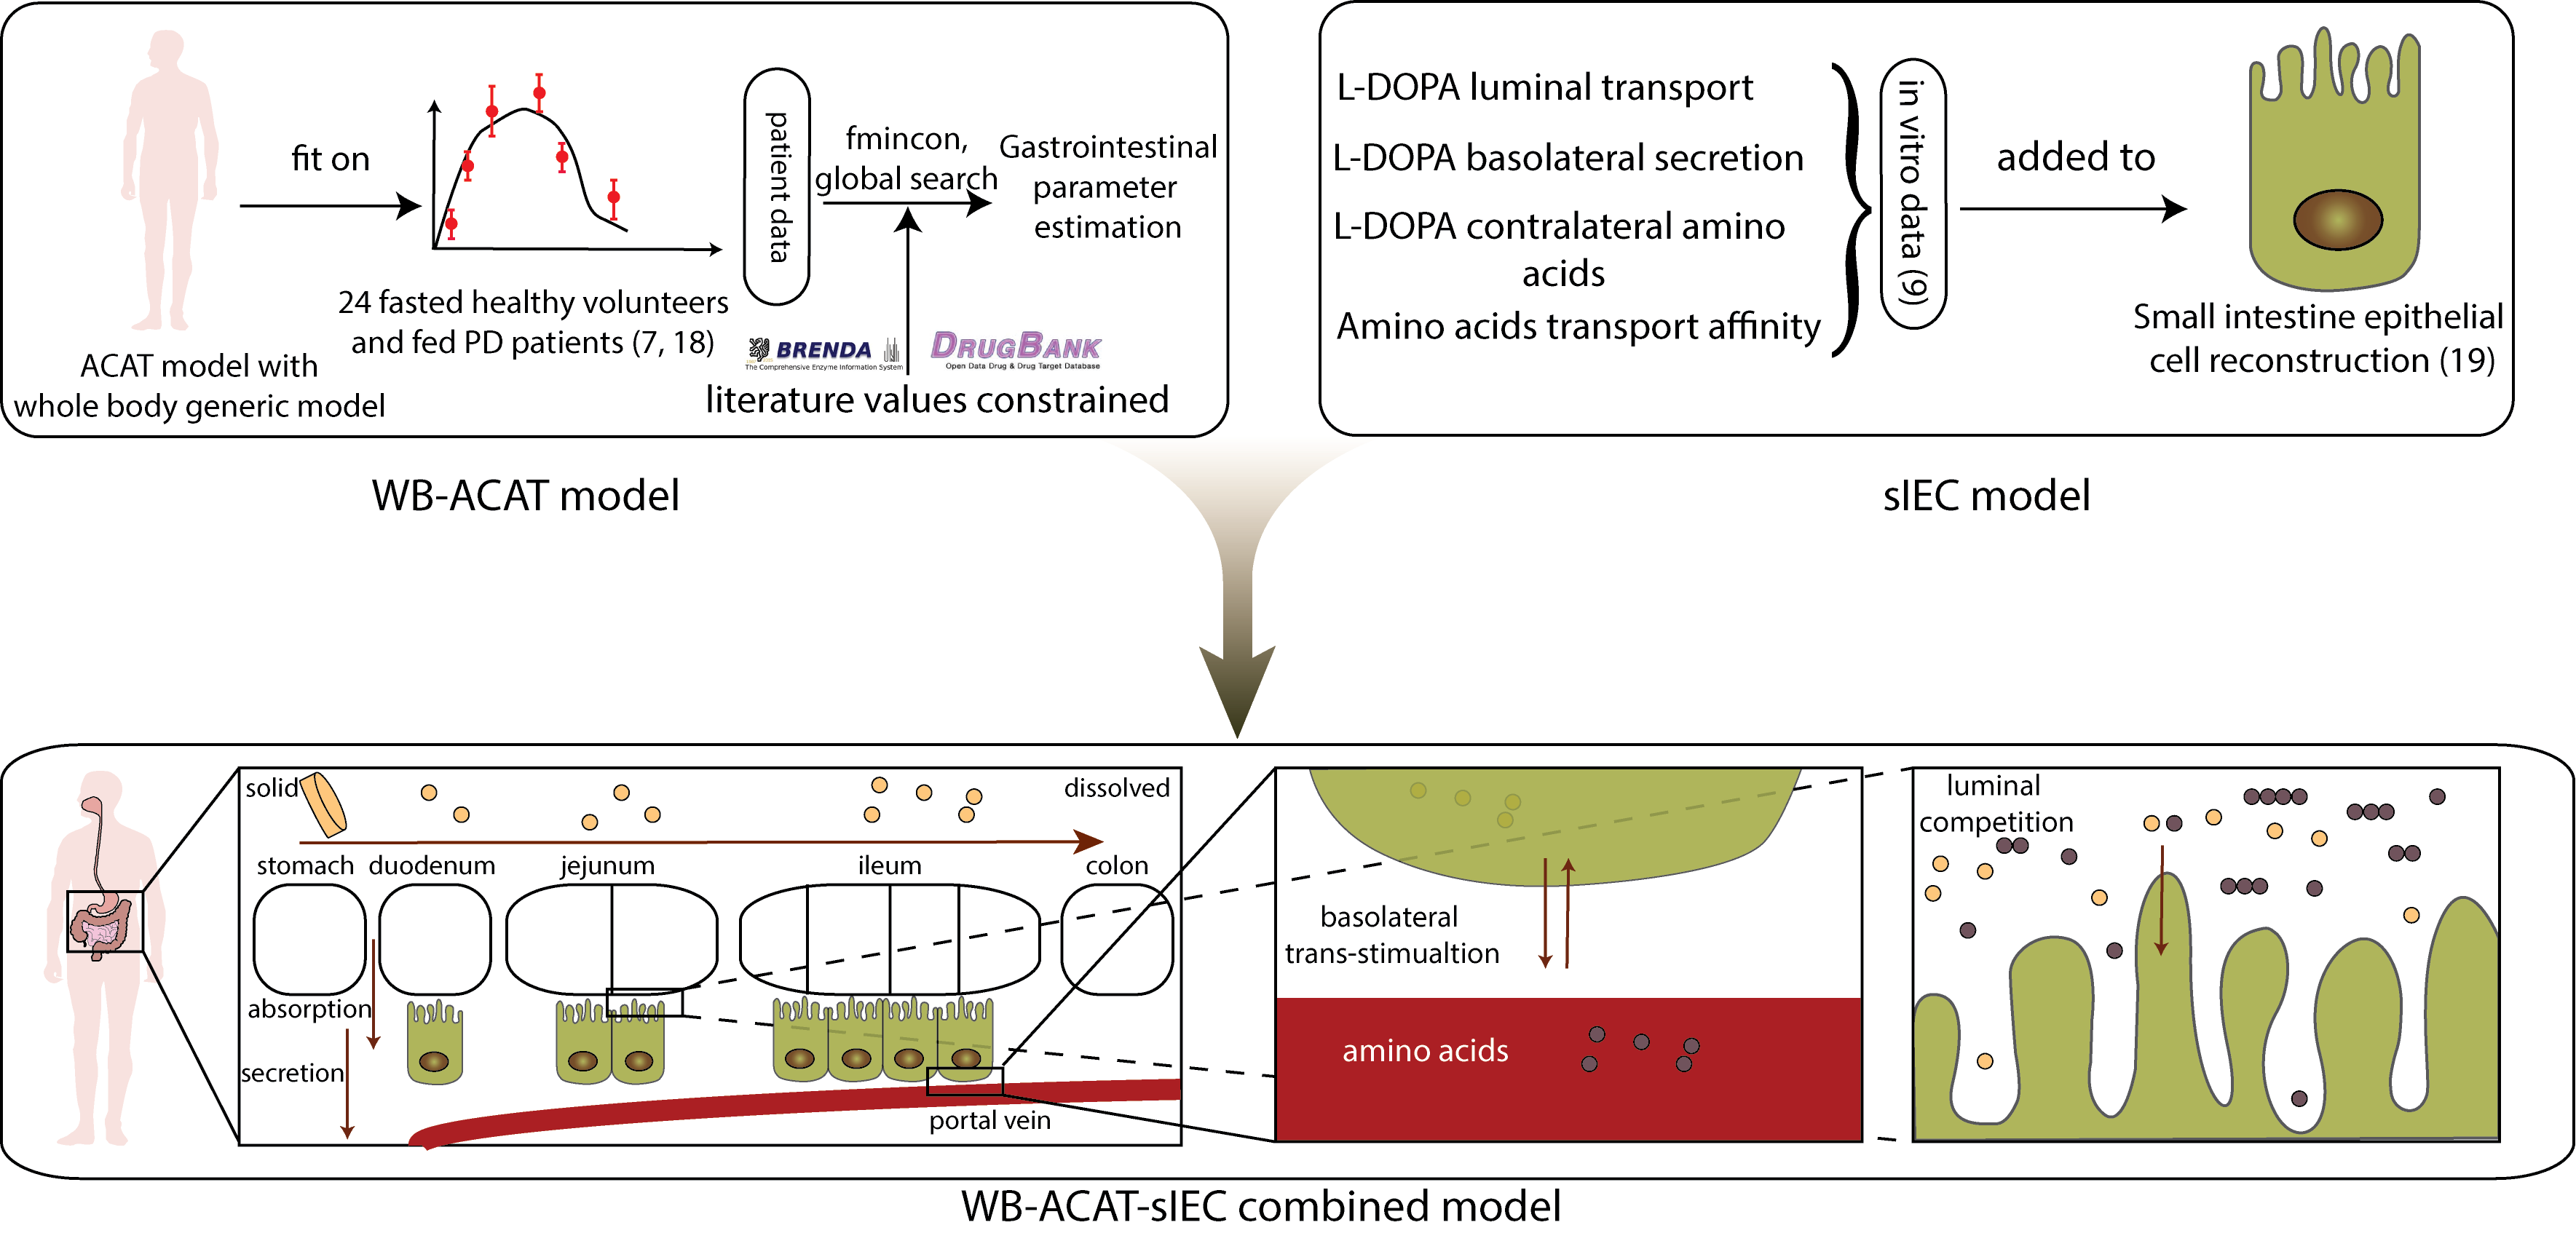
\includegraphics[width=\textwidth,height=\textheight,keepaspectratio]{levodopa/figure1.png}%Figure from images\Figure1.png
	\caption[Multiscale PBPK-COBRA model of the gut wall.]{The multiscale PBPK–COBRA model used in this study. We combined a spatially and temporally refined PBPK model (deemed WB-ACAT) of the gastrointestinal tract with seven copies of a mechanistically accurate and detailed metabolic model of small intestinal epithelial cells (sIEC). COBRA, constraint-based reconstruction and analysis; PBPK, physiologically based pharmacokinetic; WB-ACAT, whole-body advanced compartmental absorption and transit.}
	\label{fig:multiscale}
\end{figure}
To model the temporal, spatial, and metabolic effects of levodopa transport along the gastrointestinal tract, we developed a combined PBPK and COBRA model (Figure \ref{fig:multiscale}). This model combines the advantages of PBPK modeling through a comprehensive whole-body model with refined gastrointestinal absorption (WB-ACAT) model and of COBRA modelling through a mechanistically accurate and detailed small intestinal cell models (sIEC models), representing the metabolic functions of seven small intestinal segments (duodenum, two jejunum segments, and four ileum segments). The WB-ACAT model takes into account the dissolution and transit of a standard formulation of levodopa with respect to the pH and volume of each compartment, through the identified parameters of fasted and fed states. To ensure a biologically relevant set of parameters, the model was fit onto human data and constrained with values reported in the literature (Figure {fig:s1levo}-B). In addition, the global search option with the constrained optimization algorithm (Text \ref{levo:sp2}) allowed obtaining a global minimum. The subsequent absorption, metabolism, and secretion of levodopa by enterocytes were captured by the sIEC models (Figure \ref{fig:levoaa}-A) which were not added for the stomach and the colon as no absorption is assumed to take place in these two compartments. Both models were coupled using dynamic flux balance analysis (see Methods and  Figure \ref{fig:multiscale}). The WB-ACAT-sIEC model was then used to identify patients in need of dietary recommendations and to provide mechanism-based optimized diet for Parkinson's disease patients. The internal metabolites of the sIEC were assumed to be in steady state, while levodopa had a concentration rate-of-change equal to the fluxes of the dynamical model through imbalanced exchange reactions.
\subsection{Dietary intervention is needed for HY 3 and HY 4 patients}
\begin{figure}[!htp]
\centering
	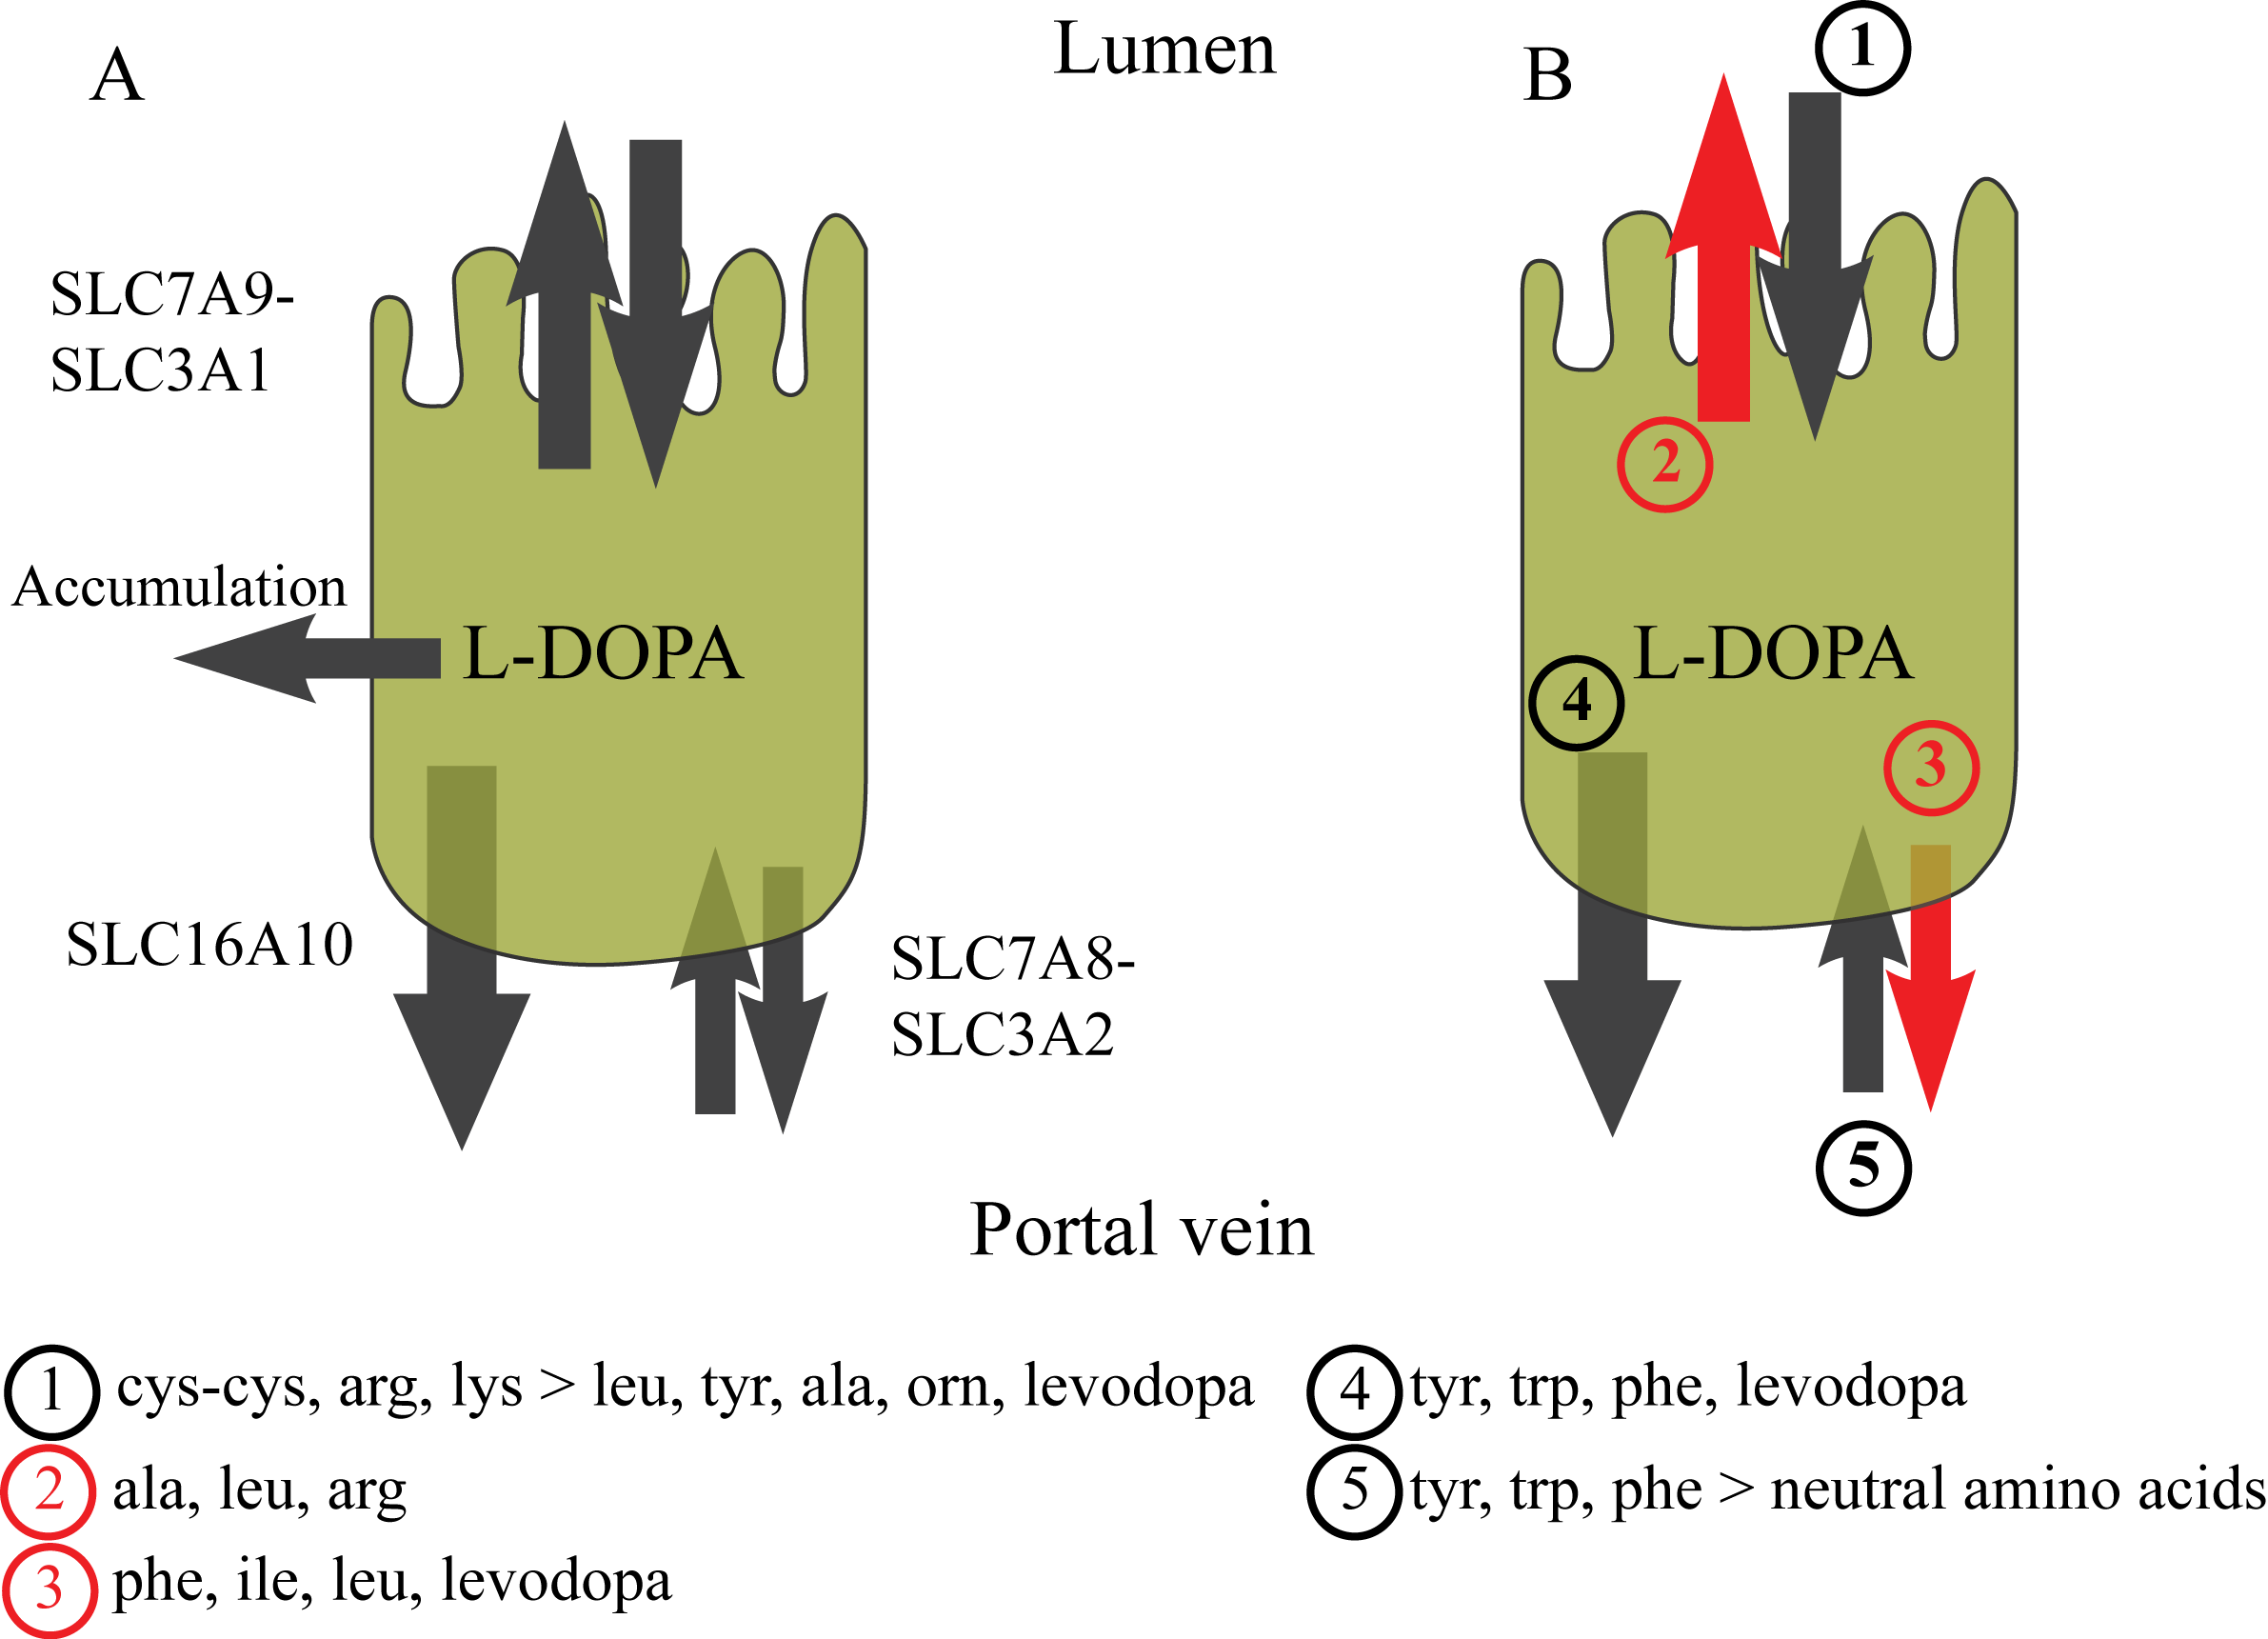
\includegraphics[width=\textwidth,height=\textheight,keepaspectratio]{levodopa/figure2.png}%Figure from images\Figure1.png
	\caption[Levodopa and amino acids affinities for enterocyte transporters.]{Levodopa and amino acids affinities for enterocyte transporters. (a) One transporter (antiporter) in the luminal side and two transporters (one antiporter and one uniporter) in the
basolateral side are involved in the absorption and secretion of
levodopa. (b) Amino acids are ordered by affinity for the transporter.
Dibasic and neutral amino acids compete for the luminal uniporter.
Aromatic amino acids uniporter is involved in the basolateral
secretion of levodopa. The basolateral antiporter exchanges
levodopa for amino acids. In both a and b, four fifths of levodopa
is secreted through the basolateral uniporter and one fifth through
the antiporter. Amino acids in the colored circle go with the
corresponding colored route.}
	\label{fig:levoaa}
\end{figure}
Using the multiscale PBPK–COBRA model, we addressed the question whether there is a particular subset of Parkinson's disease patients that would benefit the most by the recommended adjustment of dietary proteins\cite{contin2010pharmacokinetics} \cite{cereda2010low}. In particular, we investigated the pharmacokinetic profile of levodopa in a fasted state (Figures \ref{fig:s3levo} and \ref{fig:s1levo}-C, Text \ref{levo:sp4}) and in a fed state with a concomitant administration of aproteic and proteic meal (Figure \ref{fig:curves}-A). An ante cibum (a.c.) administration of 100 mg of levodopa every six hours was simulated (Figure \ref{fig:curves}-A). Each disease state on HY scale has a therapeutic window, in which the efficiency of the treatment is optimal as reflected by the control of symptoms \cite{contin2010pharmacokinetics}. A dose below the therapeutic window leads to persistence of the symptoms while a higher dose could trigger adverse effects, such as dyskinesia. Since the threshold concentrations of the therapeutic window have been determined with a 100 mg dose\cite{contin2010pharmacokinetics}, the model was simulated at the specified doses, assuming that the parameters are dose independent. In fact, nonlinear behaviour has been observed at very high, non-clinical doses\cite{lennernas1993effect}. The resulting levodopa pharmacokinetic profile in the a.c. administration state showed a higher area under the curve (AUC) in the first HY stage (colored areas in Figure \ref{fig:curves}-A). The decrease in AUC is inversely proportional to the disease stage. The simulation of the fed state with aproteic meal involved changing of physiological parameters
(Table \ref{tbl:kineticparam}). The pharmacokinetic profile showed a decrease in the maximum concentration (Cmax) and a delay in the corresponding time (Tmax). With the concomitant administration of proteic and aproteic meals, the plasma concentration of levodopa stayed below the threshold of the therapeutic window of HY 3 and HY 4
patients and did not cover optimally the therapeutic window for HY 2. Based on this information, we concluded that dietary intervention would be most beneficial for Parkinson's disease patients in HY 3 and HY 4.
\subsection{PRD improves the bioavailability of levodopa over LPD}
\begin{figure}[!htp]
\centering
	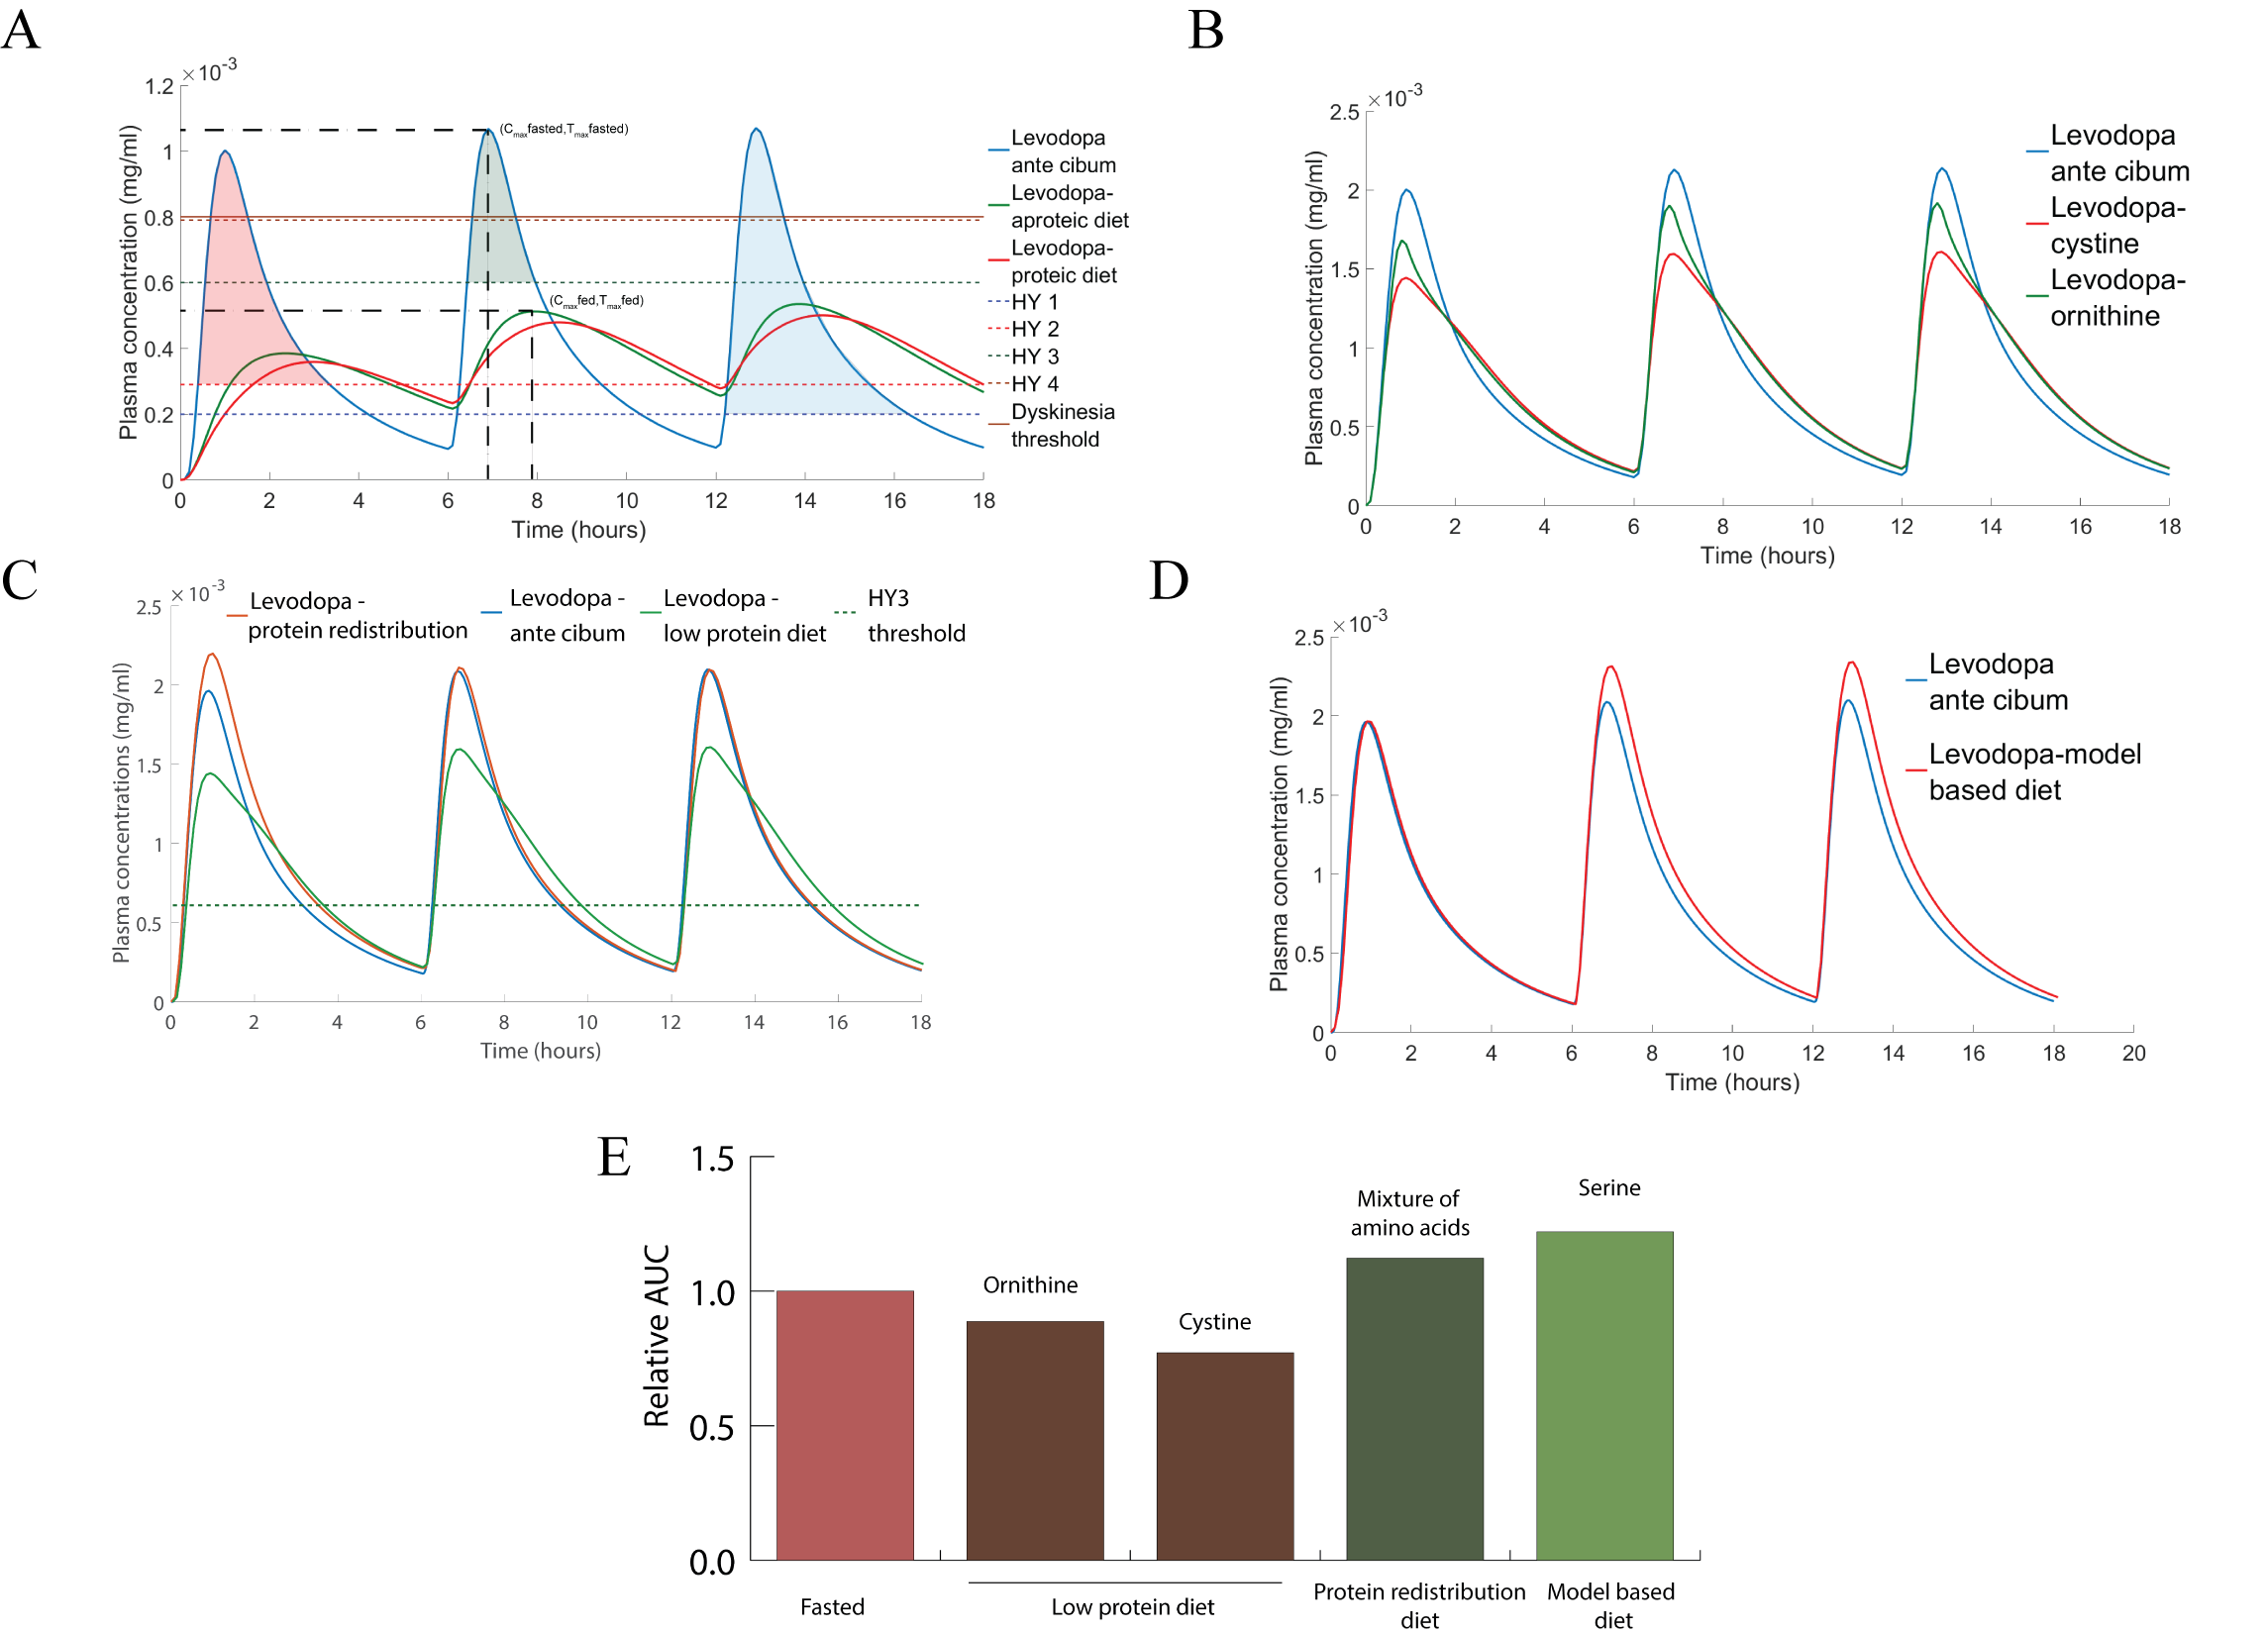
\includegraphics[width=\textwidth,height=\textheight,keepaspectratio]{levodopa/figure3.png}%Figure from images\Figure1.png
	\caption[Predicted pharmacokinetics of levodopa under different
dietary conditions.]{Predicted pharmacokinetics of levodopa under different
dietary conditions. (a) a.c., proteic, and aproteic meals influence on
the pharmacokinetic profile of levodopa. The efficacy threshold
values for the different disease progression stages were plotted in
dashed lines on Hoehn and Yahr scale (HY1 to HY 4). The more
advanced the stage, the higher the levodopa concentration threshold.
The AUC corresponding to HY1 in the fasted state is the blue
area, HY 2 is the red area, and HY 3 is the green area (b) The
pharmacokinetic profile of levodopa under LPD diet. (c) The
pharmacokinetic profile of levodopa under PRD diet, LPD diet and
a.c. administration. (d) The pharmacokinetic profile of levodopa with
the model proposed serine-rich diet, which can increase the
bioavailability of levodopa. (e) Relative variation of the AUC of
levodopa under different dietary conditions in comparison to the
fasted state. a.c., ante cibum; AUC, area under the curve; LPD,
Low-protein diet; PRD, protein redistribution diet.}
	\label{fig:curves}
\end{figure}
In later stages of Parkinson's disease, the reported superiority of PRD over LPD may be due to an increase in bioavailability of levodopa. To test this hypothesis, the pharmacokinetic profile of levodopa under both LPD and PRD was simulated. In the LPD setting, 0.8 g amino acids per kg body weight were administered \textit{in silico} together with 200 mg of levodopa three times a day (t.i.d.) every 6 h. LPD
assumes that levodopa dose is taken before the meal; hence, none of the physiological parameters (Table \ref{tbl:kineticparam}) were effective in the simulation. Since LPD and PRD are recommended in late-stage Parkinson's disease patients, with pronounced impairment of gastric emptying that can go up to 7 h \cite{hardoff2001gastric}, it is assumed that the last meal with < 0.8 g/kg of body weight of proteins is still present in the small intestine. 
To account for the different affinities of amino acids for the luminal transporter and the subsequent competition with levodopa, cystine and ornithine were first simulated as these amino acids have the highest and lowest affinity (Figure \ref{fig:levoaa}-B, Table \ref{tbl:kineticparam}), respectively. The AUC above the efficacy threshold
decreased by 11.24\% for ornithine and by 22.91\% for cysteine in comparison to the a.c. administration (Figure \ref{fig:curves}-B).
PRD is based on the redistribution of the daily protein allowance to the last meal, for the latest stages of Parkinson's disease \cite{cereda2010low}. It has been demonstrated that gastric emptying rate (GER) decreases severely in the latest stage of Parkinson's disease. Moreover, the
kinetics of amino acids in the plasma, after protein ingestion, are higher than the baseline after 8 h \cite{bos2003postprandial}. We consequently assumed that a high fraction of amino acids is present in the systemic circulation and in the portal vein, particularly, when the next levodopa dose is taken the following day. In particular, the transstimulation effect on levodopa secretion by amino acids was captured with the sIEC basolateral transporters (Figure \ref{fig:couplemethod}). The simulation showed that a higher flux through the basolateral antiporter induced a higher bioavailability of levodopa, which is reflected by the increase of AUC above the efficacy threshold throughout the day (11.23\%) in comparison to the fasted state
(Figure \ref{fig:curves}-C). Taken together, these results support the observed superiority of PRD over LPD to increase the systemic bioavailability of levodopa, which is reflected in our simulations by the cumulative increase in the AUC (34\%).
\subsection{Impaired gastrointestinal processes reduced levodopa efficacy}
\begin{figure}[!htp]
\centering
	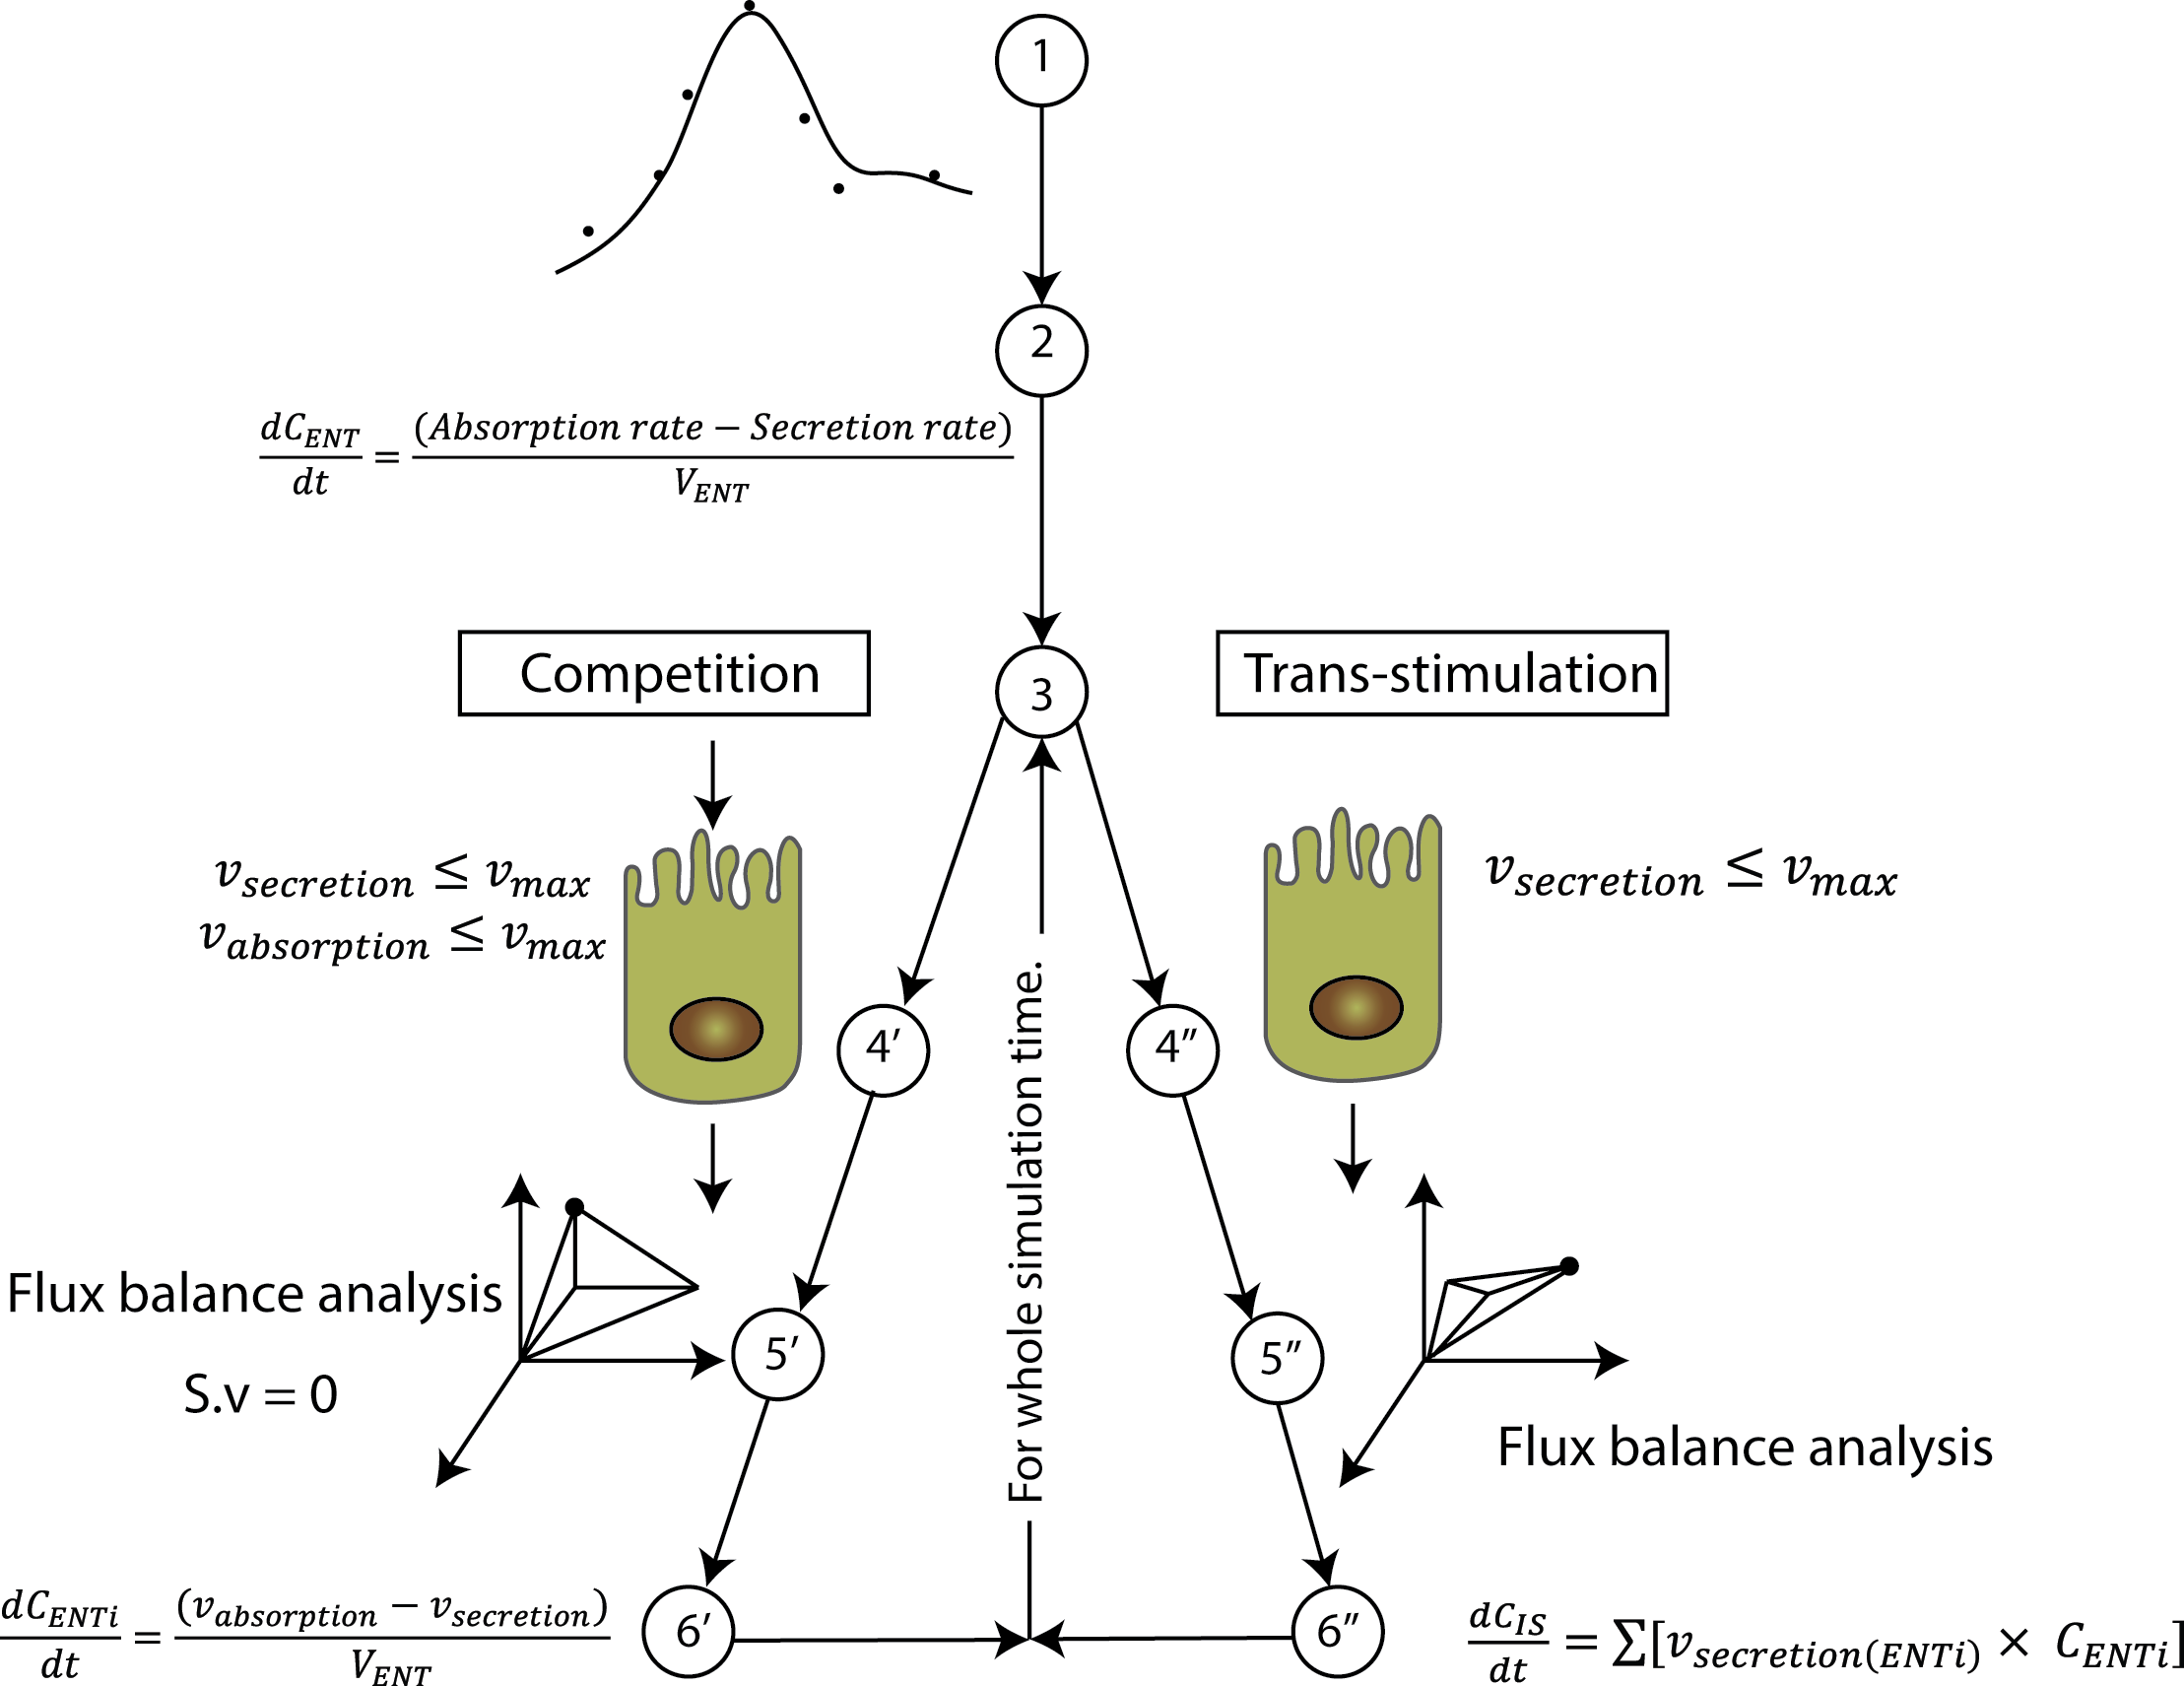
\includegraphics[width=\textwidth,height=\textheight,keepaspectratio]{levodopa/figure4.png}%Figure from images\Figure1.png
	\caption[Multiscale modeling of the WB-ACAT-sIEC model for the absorption of levodopa by the small intestine.]{Multiscale modeling of the WB-ACAT-sIEC model for the absorption of levodopa by the small intestine. The key steps of the sequential
coupling algorithm are illustrated. Step 1 (PBPK modeling): the physiological parameters of levodopa distribution were identified by fitting data
from healthy individuals45 onto the WB-ACAT model. Step 2 (PBPK modeling): the WB-ACAT model, together with the obtained parameters, was
simulated for one-time step. Steps 3 (PBPK modeling): the flux values were retrieved, depending on the competition or trans-stimulation mode,
for absorption and secretion reactions/metabolites that are in common between the WB-ACAT and the sIEC models. Step 4 (COBRA modeling): as
the WB-ACAT model captured seven distinct sIEC segments, the flux values for each segment were set as upper bound on the one sIEC model
corresponding to this segment. Step 5 (COBRA modeling): for each sIEC model, FBA was performed with the levodopa luminal uptake reaction or
basolateral secretion as objective function, depending on the mode. Step 6 (COBRA modeling): the obtained FBA flux values for each sIEC model
were set as parameters for the derivatives in the corresponding sIEC segments of the WB-ACAT model. The new rates initialized the next time
step in the PBPK modeling (Step 3). Numbers with single and double subscript correspond to competition and trans-stimulation, respectively.
COBRA, constraint-based reconstruction and analysis; PBPK, physiologically based pharmacokinetic; sIEC, small-intestine epithelial cell; WB-ACAT,
whole-body advanced compartmental absorption and transit.}
	\label{fig:couplemethod}
\end{figure}
The slower gastric motility, induced by food and several conditions, decreases the bioavailability of orally absorbed drugs \cite{contin2010pharmacokinetics}, including levodopa. We identified the parameter for GER for the fasted and the fed state based on a two-occasion study \cite{contin2010pharmacokinetics} (see Methods for details, Table \ref{tbl:kineticparam}). We used the fitted GER to simulate the kinetics of levodopa in Parkinson's disease patients with the concomitant administration of food (Figure \ref{fig:curves}-A). The parameter sensitivity analysis with respect to levodopa plasma concentrations showed that the top 5 ranking parameters
among the 243 whole-body parameters were gastrointestinal parameters (Figure {fig:s4levo}, Table \ref{tbl:tbls4}).
These findings highlight the importance of oral absorption in the dynamics of levodopa and consequently the emergence of fluctuations in the motor response.
\subsection{Ranking of amino acids effects toward levodopa bioavailability revealed serine-rich diet as a potential augmenting diet for levodopa \textit{in silico}}
\begin{figure}[!htp]
\centering
	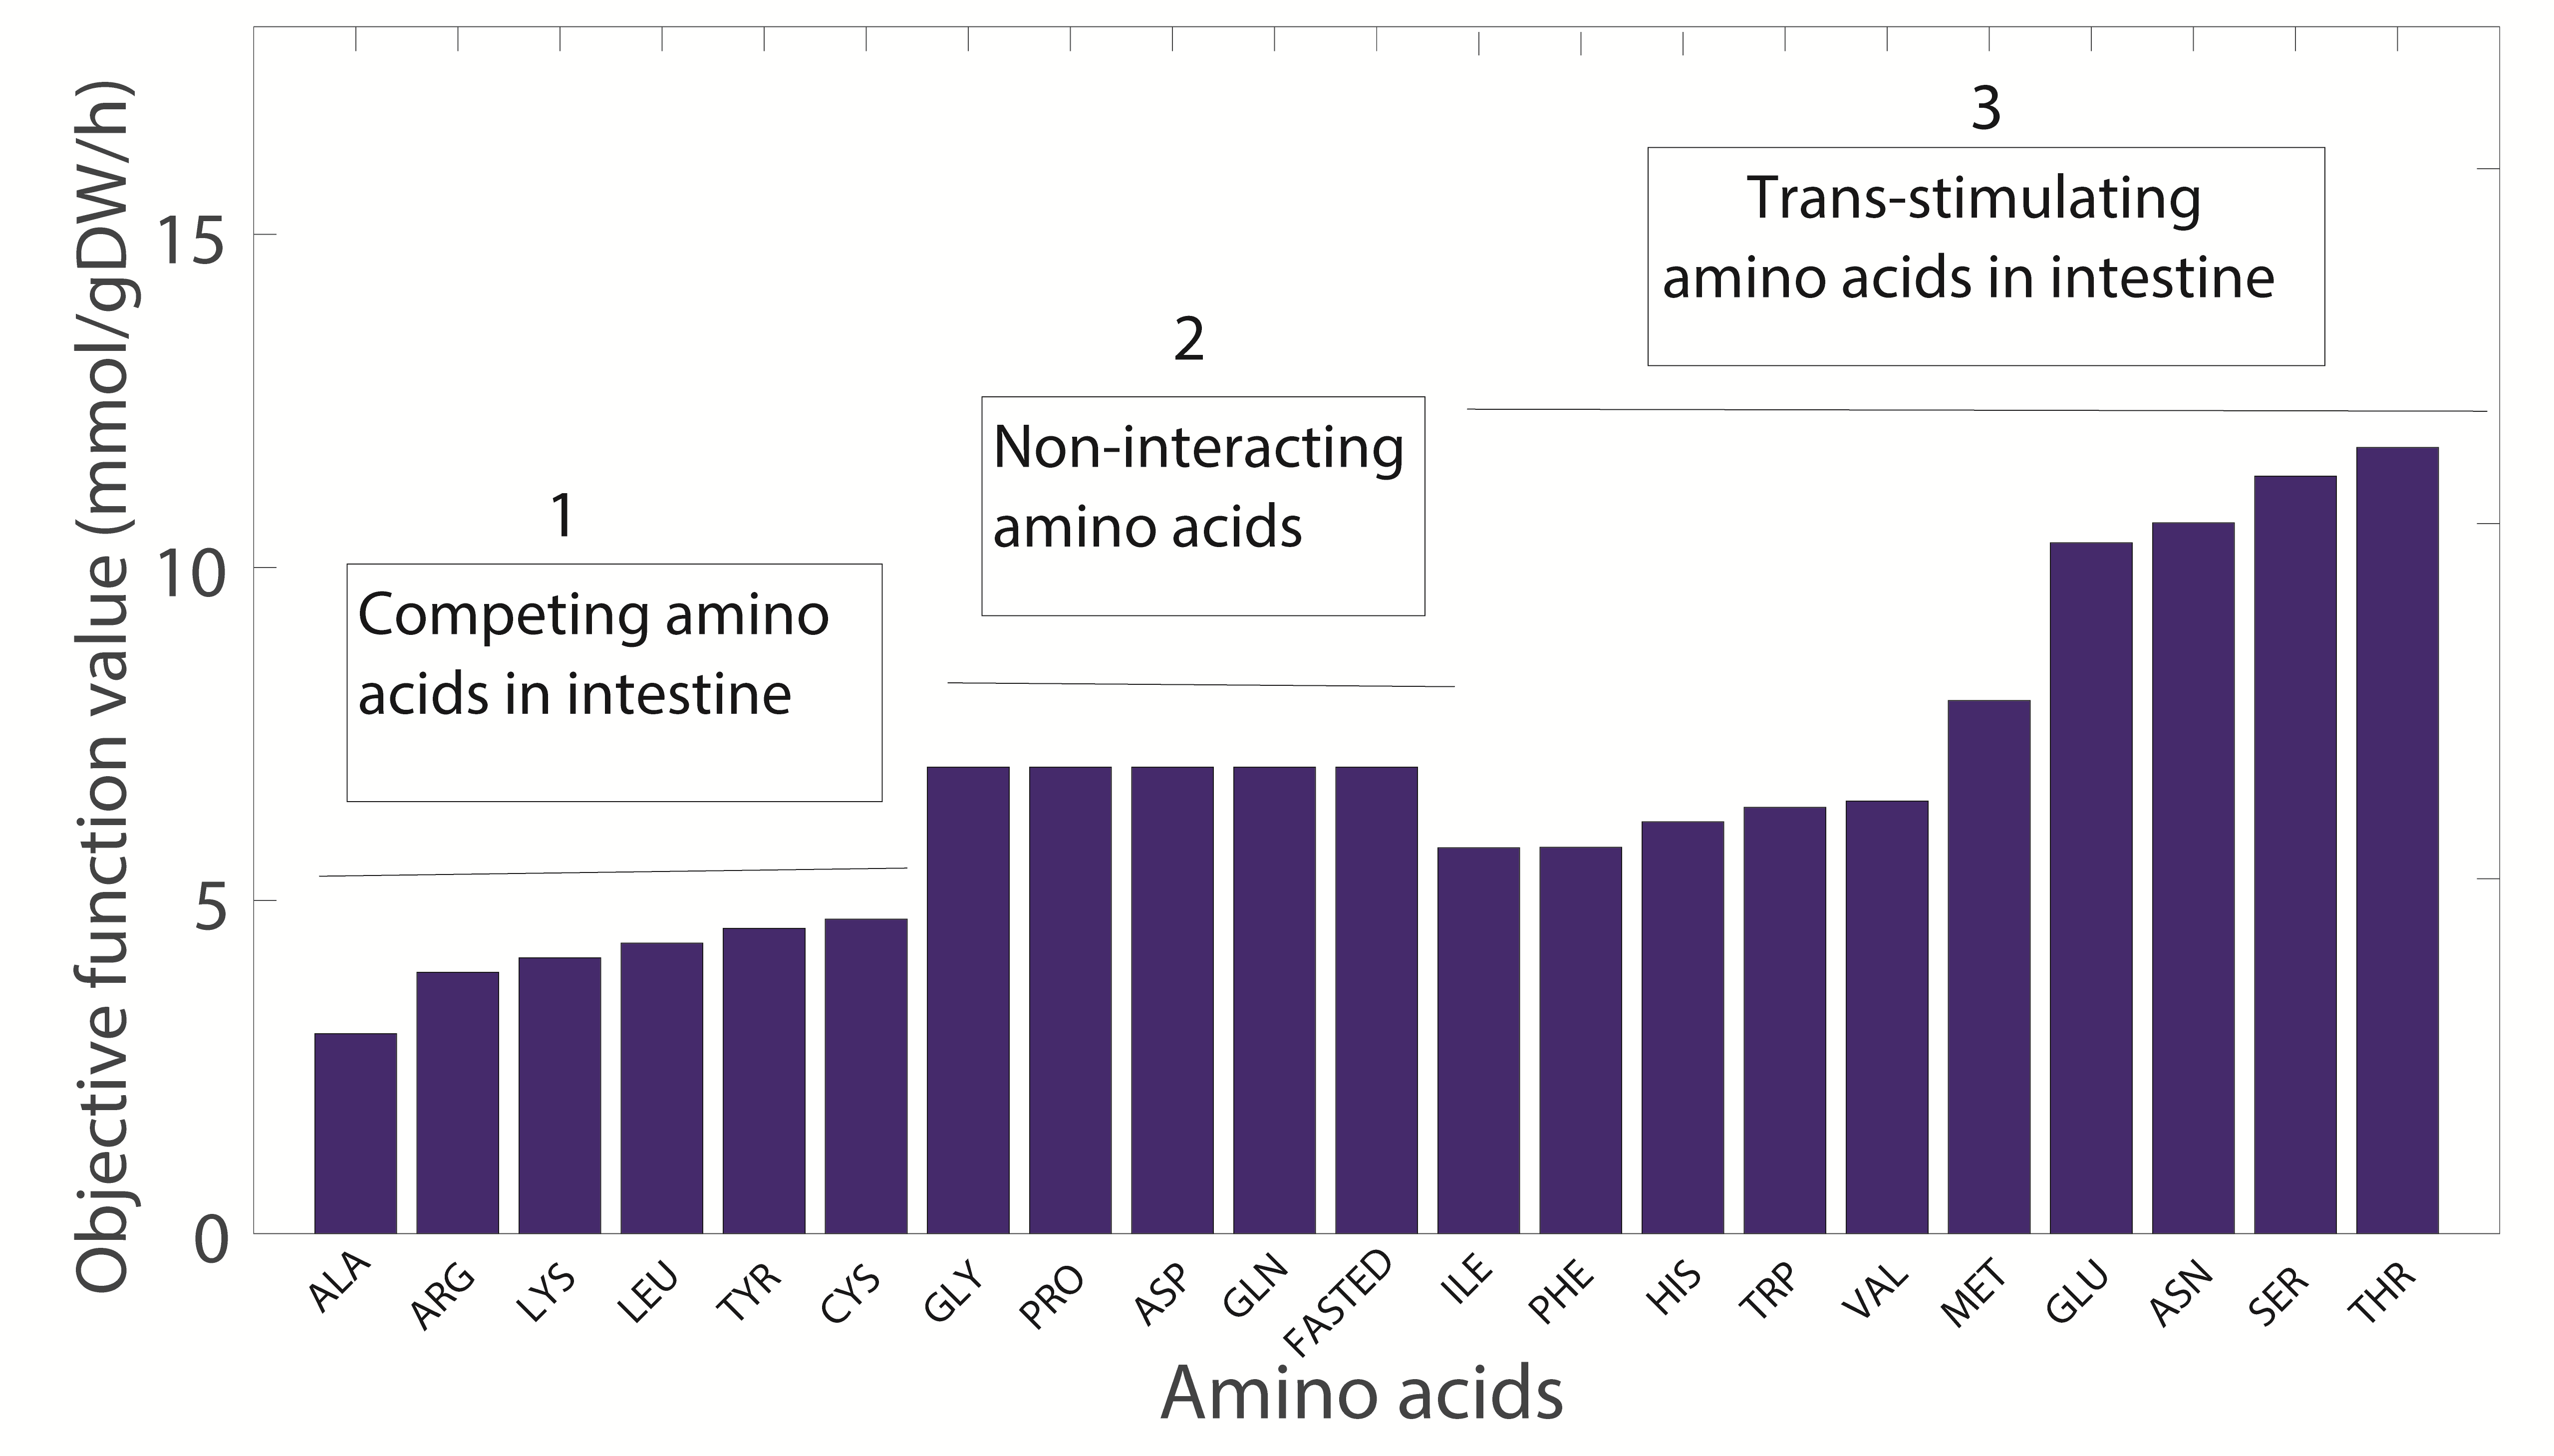
\includegraphics[width=\textwidth,height=\textheight,keepaspectratio]{levodopa/figure5.png}%Figure from images\Figure1.png
	\caption[Ranking of amino acids with respect to the levodopa
fraction that reaches the brain.]{Ranking of amino acids with respect to the levodopa
fraction that reaches the brain. Amino acids with lowest ranking
were those which competed with levodopa in the intestine.
A second set of amino acids did not interact with levodopa and,
consequently, the levodopa pharmacokinetics was identical to those
of the fasted state. A third set improved the levodopa absorption
and also did not compete with amino acid uptake by the brain. The
objective function in the simulations was the levodopa transport
reaction across the blood–brain barrier using an extended sIEC
model, to which a kidney and brain compartment with the
corresponding levodopa transport reactions were added. sIEC,
small-intestine epithelial cell.}
	\label{fig:aarank}
\end{figure}
The competition and trans-stimulation between levodopa and amino acids take place mainly in the gut, brain, and kidneys\cite{verrey2000glycoprotein}. To capture also these interactions in our WB-ACAT-sIEC model, we extended the sIEC model by a kidney and brain compartment (Table \ref{tbl:tbls5}) and included the corresponding levodopa transport reactions (sIEC*, Text \ref{levo:sp5}). To simulate this interaction between the three organs in the levodopa bioavailability, we set the levodopa influx rate to the intestinal lumen to the arbitrary value of 15 mmol/g of dry weight/h (Table \ref{tbl:tbls6}), of which 66\% could reach the systemic circulation in the fasting state and
30\% of the absorbed fraction was eliminated by the kidneys, in accordance with experimental data\cite{contin2010pharmacokinetics}. We then simulated the simultaneous administration of levodopa with the different amino acids by selecting as objective function the brain transport reaction for levodopa. This simulation allowed us to systematically determine, which amino acid would lead to a higher flux of levodopa transported to the brain and thus, could result in a better clinical outcome. We found that threonine, serine, and asparagine resulted in the highest brain bioavailability of levodopa (Figure \ref{fig:aarank}). To our knowledge, these amino acids have not been reported to compete with levodopa in the small intestine and in the brain. Moreover, the amino acids were predicted to compete with levodopa for elimination in the kidneys and trans-stimulate levodopa secretion from the intestinal lumen.
It has been shown that serine improves dopamine production \cite{gelfin2012d}.
Consequently, we ranked serine as the amino acid with the highest contribution to levodopa bioavailability.
\begin{table}[h]
\caption[Fed versus fasted state physiological parameters.]{Fed versus fasted state physiological parameters.}
\begin{center}
	\begin{tabular*}{\textwidth}{l @{\extracolsep{\fill}} lll}
	\hline
	Parameters	                 & Fasted/ante cibum & Fed \\ 
	\hline
	GER                          & 3.96 per h        & 0.33 per h \\
	Stomach volume               & 50 ml             & 1000 ml \\
	Colon volume                 & 1000 ml           & 7000 ml \\
	Small intestine transit rate & 2.1 per h         & 0.57 per h \\
	Gastric pH                   & 2                 & 5 \\
	\hline
	\end{tabular*}
\end{center}
\caption*{Abbreviation: GER, gastric-emptying rate.
The physiological parameters in fasted and fed state were taken from the
literature.49 The gastric-emptying rate was estimated by sequential fit
on levodopa plasma concentrations in fasted and fed states onto the
WB-ACAT model.}
\label{tbl:kineticparam}%descriptive label to refer to figure in text
\end{table}
Using the WB-ACAT-sIEC model, we predicted that the addition of serine in the systemic circulation could improve the bioavailability of levodopa as shown by the increase of the AUC above the efficacy threshold (22.02\%) (Figure \ref{fig:curves}-D,E). The subsequent increase of amino acids concentration in the plasma improved the bioavailability of the next dose through a higher absorption in the basolateral side of the seven compartments of the small intestine. Taken together, we propose that a serine-rich meal after a levodopa dose could improve the brain bioavailability of levodopa.
\section{Discussion}
Motivated by the observation that protein-containing meals can alter the levodopa bioavailability and thus the motor symptoms of Parkinson's disease patients, we developed a multiscale PBPK–COBRA model of the gastrointestinal tract. We then investigated different dietary strategies. Our key results include: (i) late-stage, levodopa-treated Parkinson's disease patients would benefit the most by dietary intervention; (ii) PRD but not LPD improved the bioavailability of levodopa; (iii) gastrointestinal transit and loss of levodopa explained most of the variability in levodopa bioavailability; and (iv) serine-rich diet could increase the brain levodopa bioavailability. Taken together, we demonstrate that computational modeling could add further mechanistic insight into the diet-levodopa interactions and may be used to propose Parkinson's disease patient-specific dietary intervention strategies.
\subsection{The combined model: construction, assumptions and validation}
In this study, we developed a spatially, temporally, and mechanistically detailed model of the human gastrointestinal tract  (Figure \ref{fig:multiscale}) by combining two powerful modeling techniques: PBPK and COBRA. In comparison to the other efforts\cite{krauss2012integrating}, we demonstrate here that this hybrid modeling technique can be further expanded by including more refined PBPK models (i.e., the ACAT model), as well as by integrating more than one stoichiometric metabolic models (i.e., seven sIEC models)  (Figure \ref{fig:multiscale}). Importantly, the simulation settings were consistent with literature reports, such as levodopa being absorbed equally in all the parts across small intestinal\cite{lennernas1993effect}, while amino acids were only absorbed in the proximal jejunum (jejunum 1 and 2 in the model)\cite{adibi1967kinetics}. The kinetic profile of levodopa with concomitant administration of proteic diet in late-stage patients (Figure \ref{fig:curves}-A) matched the profile of levodopa of one case patient with gastrointestinal resection\cite{nagayama2015pharmacokinetics}, which suggests that inhibitory amino
acids completely block the access of levodopa to the intestinal transporters in the sites of absorption. These findings show that the proposed hybrid modeling approach  (Figure \ref{fig:multiscale}) provides a powerful tool to assess diet–drug interactions, which requires interrogation at the physiological, as well as biochemical level \cite{van2011systems}.
\subsection{Late-stage, levodopa-treated Parkinon's disease patients would benefit the most by dietary intervention}
In the last stages of Parkinson's disease, levodopa-treated patients experience fluctuations in the motor response\cite{contin2001levodopa}. The on-off phenomena are correlated to inadequate concentrations of levodopa reaching the brain. Since the impairment of the gastrointestinal motility in Parkinson's disease \cite{fasano2015gastrointestinal} increases with disease progression, the erratic absorption of levodopa, especially with diet, is one of the factors causing motor fluctuations. As our model showed (Figure \ref{fig:curves}-A), the decrease in levodopa absorption was lower with respect to the therapeutic threshold in early-stage patients with low impairment of gastric emptying, while it substantially decreased the bioavailability of levodopa in later stages of Parkinson's disease. These results are in agreement with reported clinical trials\cite{contin2001levodopa}, and routine, where HY 3 and HY 4 patients are recommended to follow a dietary plan, such as PRD and LPD.
\subsection{Gastrointestinal transit and loss of levodopa explained most of the variability in levodopa bioavailability}
Constipation is a clinical symptom associated with Parkinson's disease, particularly at the later stages\cite{fasano2015gastrointestinal}. Overall, the GER is inversely proportional to the disease stage\cite{doi2012plasma}. In addition, levodopa is degraded in the stomach and intestine lumen as a consequence of gut microbiota\cite{sousa2008gastrointestinal}, luminal enzymes \cite{nutt1984off}, and chemical degradation\cite{agoram2001predicting}.
The higher residence time of levodopa in the gastrointestinal tract, caused by the slower GER, leads to a higher degraded fraction. The predicted decrease in the maximal concentration (Cmax) was the result of the combination of a slow GER and the luminal degradation (Figure \ref{fig:curves}-A). The parameter sensitivity analysis showed that gastric and intestinal processes were the most influential factors for levodopa bioavailability (Table \ref{tbl:tbls4}, Figure {fig:s4levo}). The GER has been shown to be the main parameter that induces a delay in levodopa
absorption\cite{doi2012plasma}. Our observation is further consistent with the reported decrease in levodopa efficiency with pH34 and \textit{Helicobacter pylori} infection \cite{hashim2014eradication} \cite{pierantozzi2006helicobacter}. The levodopa loss in the stomach also motivated approaches that bypassed the gastrointestinal tract \cite{foltynie2013impact} and the intestine\cite{nutt1984off}, as well as provides a rationale for investigational prokinetics for Parkinson's disease patients\cite{sanger2009gsk962040}.
The absorptive profile of levodopa has been reported to show multiple peaks in plasma and an erratic absorption. Such erratic kinetics were not observed in the simulations (Figure \ref{fig:curves}-A), which suggests that GER is a time-dependent parameter, as suggested previously\cite{waller1991oral}. Our results suggest that the plasmatic concentrations of levodopa were higher 2 h after the administration than the a.c. administration. This observation could be explained by the absorption of levodopa in the ileum, where the competition with amino acids has not been reported\cite{adibi1967kinetics}. This finding indicates a role of ileal levodopa absorption in the formation of delayed plasmatic peaks.
\subsection{PRD but not LPD improved the bioavailability of levodopa}
It has been shown that PRD had a better clinical outcome than
LPD\cite{cereda2010low}. In silico, the PRD had also a better performance due to the improved bioavailability of levodopa (Figure \ref{fig:curves}-B,C). A combination of factors has been suggested to result in the superiority of protein redistribution diet\cite{cereda2010low}. In LPD, we showed that competing amino acids decreased the levodopa peak (Figure \ref{fig:curves}-A,B). It is likely that the decrease is more pronounced with impaired GER.
A slower GER potentializes the loss of levodopa by competition
through exposing the dietary proteins to intestinal peptidases for
longer periods of time, thus releasing amino acids. It has been
shown that in healthy volunteers after protein intake, a minor part
of the diet is transformed into free amino acids in the small
intestine, while the major part forms di- and tri-peptides and
is absorbed by PEPT1\cite{adibi1973protein}. A clinical trial conducted on healthy volunteers showed no difference in the pharmacokinetics of levodopa when absorbed alone or with a solution of proteins, which questioned the influence of the gastrointestinal processes on the absorption of levodopa \cite{robertson1991influence}. With most proteins being transformed into non-competing peptides, levodopa is not subjected to competition for luminal transporters. Thus, the delay in GER exacerbates the competitive potential of dietary amino acids, which leads to higher loss of levodopa in the small intestine.
\subsection{Serine-rich diet could increase the brain levodopa bioavailability}
Basolateral amino acids, mimicking the post prandial state, have been shown to trans-stimulate the secretion of levodopa\cite{camargo2014molecular}. The latter finding provides opportunities for augmenting dietary intervention. Serine supplementation increased \textit{in silico} the bioavailability of levodopa for Parkinson's disease patients with moderately impaired GER (Figure \ref{fig:curves}-D). Furthermore, the exchange of levodopa with amino acids could be a clearance route for amino acids, thus, preventing further competition in the brain (Figure {fig:s5levo}). Serine also modulates the activation of N-methyl-D-aspartate
class of glutamate receptors (NMDARs), which were hown to be involved in dopamine synthesis and release\cite{gelfin2012d}. Thus, serine-rich diet could improve the absorption of levodopa and the production of dopamine\cite{growdon1982effects}. Recently, a clinical study on late-stage Parkinson's disease patients has demonstrated a higher bioavailability of levodopa and an improvement of ‘on’ times with soybean \cite{nagashima2016effects}. Given that soybean is mainly composed of 2331 mg/100 g of glutamate, 1411 mg/100 g of aspartate, 982 mg/100 g of arginine, and 687 mg/100 g of serine, it appears that inhibitory effects of arginine are counteracted by the predicted beneficial effects of serine and glutamate, while aspartate was predicted to be neutral (Figure \ref{fig:aarank}). This finding suggests that a cumulative, dose-dependent effect of amino acids on the ranking scale that we have developed (Figure \ref{fig:aarank}), in a given diet, is a good assessment of its effects on the pharmacokinetics of levodopa. 
A higher bioavailability of levodopa allows (i) a better clinical outcome, (ii) a decrease in the daily dose with (iii) the subsequent decrease in adverse reactions.
Taken together, we demonstrate in this study that the combination of genome scale and dynamical models can be used to assess the diet–drug interactions and can provide a valuable tool to design nutritional intervention strategies.
\section*{Acknowledgments}
We thank Drs Swagatika Sahoo and Maike Aurich for valuable discussions and
technical assistance. This study was funded by Luxembourg National Research Fund
(FNR), an ATTRACT programme grant (FNR/A12/01), and through the National Centre
of Excellence in Research (NCER) on Parkinson's disease.
%Path to chapter

\chapter{Dynamic load balancing enables fast and parallel computation of large-scale metabolic models.}
\label{ch:chapter4}
\chaptermark{dynamic load balancing of metabolic models}%Short description for page header
{\setstretch{1.0} \textit{Manuscript in preparation. Poster presentation at the 2017 
\href{https://www.sbhd-conference.org/2017/images/Alphabetical_list_poster_presenters-SBHD_2017.pdf}{International Conference on Systems Biology of Human Disease in Heidelberg, Germany.}
} \par}%Paper reference, note, other. Can remove. Single line space.
\section*{Abstract}
{\setstretch{1.0}  
GSMMs of living organisms are used in a wide variety of applications pertaining to health and bioengineering. They are formulated as LP problems that are oftentimes under-determined. FVA characterizes the alternate optimal solution (AOS) space enabling thereby the assessment of the solution's robustness. fastFVA (FFVA), the C implementation of MATLAB FVA, allowed to gain substantial speed up, although the parallelism was managed through MATLAB. We present veryfastFVA (VFFVA), a pure C implementation of FVA, that relies on a hybrid MPI/OpenMP management of parallelism. The flexibility of VFFVA allowed to gain consequent speedup factors and to decrease memory usage 14 fold in comparison to FFVA. Finally, VFFVA allows to process a higher number of GSMMs in faster times accelerating thereby biomedical modeling and simulation.
\par}%single line space

\newpage
\section{Introduction}
Modeling and simulation of biological systems gained tremendous interest thanks to the increasing predictive ability of the modeled systems in healthcare and in the biotechnology industry \cite{gottstein2016constraint,oyaas2017genome}. Microbial and human systems are most amenable to modeling given the wealth of data in the literature along with the development of computational methods. \\
Particularly, COBRA methods enable the reconstruction of the metabolism of biological systems \textit{in silico} as linear programs \cite{o2015using}. Subsequently, an objective function of the system is formulated and optimized for e.g., biomass yield, metabolite production. Although the objective is uniquely determined, the set of corresponding solutions forms the space of alternate optimal solutions (AOS) that describe the possible conditions in which the optimal objective is achievable. The AOS space is quantified using flux variability analysis (FVA) \cite{mahadevan2003effects}, which provides a range of minimum and maximum values for each variable of the system. Biologically, these values overlap with the fitness of a given system to achieve optimality and allow to validate the metabolic phenotype through matching the empirical ranges with the FVA bounds.
fastFVA (FFVA) \cite{gudmundsson2010computationally}, a recent implementation of FVA gained tremendously in speed over the \texttt{fluxvariability} COBRA toolbox MATLAB function \cite{becker2007quantitative}. Two main improvements were the driving factor of the gained efficiency: first, the C implementation of FVA which allowed a higher flexibility using the CPLEX C API in comparison to MATLAB. The second was the use of the same LP object, which avoided solving the problem from scratch in every iteration, thereby saving presolve time. FFVA is compiled as MATLAB Executable (MEX) file, that can be called from MATLAB directly.\\
Yet, given the exponentially growing size of the metabolic models, FFVA is ran in parallel in most cases. Parallelism simply relies on allocating the cores through MATLAB \texttt{parpool} function and running the iterations through \texttt{parfor} loop. The load is statically balanced over the workers such as they process an equal amount of iterations. Nevertheless, the solution time varies greatly between LPs which does not guarantee an equal processing time among the workers in static load balancing. Oftentimes, the workers that were assigned a set of fast-solving LPs, process their chunk of iterations and stay idle, waiting to synchronize with the remaining workers, which can result in less efficient run times.
We present veryfastFVA (VFFVA), a pure C implementation of FVA, that has a lower level management of parallelism over FFVA. The program is provided as a standalone, that does not rely on MATLAB thereby offering an open source alternative for constraint-based biological analysis. The major contribution lies in the management of parallelism through a hybrid OpenMP/MPI, for shared memory and non-shared memory systems respectively, which offers great flexibility and speedup over the existing implementations. While keeping the up-mentioned advantages of FFVA, load balancing in VFFVA was scheduled dynamically \cite{suss2008common} in a way to guarantee equal run times between the workers. The input does not rely on MATLAB anymore as the LP problem is read in the industry standard $.mps$ file, that can be also obtained from the classical $.mat$ files through a provided converter. The improvements in the implementation allowed to speed up the analysis by a factor of three  and reduced memory requirements 14 fold in comparison to FFVA and the Julia-based distributedFBA implementation \cite{heirendt2016distributedfba}, in a similar parallel setting.\\
Taken together, as metabolic models are steadily growing in number and complexity, their analysis requires the design of efficient tools. VFFVA allows to make the most of modern machines specifications in order to run a greater amount of simulation in less time thereby enabling biological discovery. 
\section{Material and methods}
\subsection{Flux variability analysis}
The LP problem representing the metabolic model has $n$ reactions that are bounded by lower bound $lb_{(n,1)}$ and upper bound $ub_{(n,1)}$ vectors.  The matrix $S_{(m,n)}$ represents the stoichiometric coefficients of each of the $m$ metabolites involved in the $n$ reactions. The system is usually constrained by $S.v=0$ to represent the steady-state, also referred to as Flux Balance Analysis (FBA) \cite{orth2010flux}. An initial LP optimizes for the objective function of the system to obtain a unique optimum e.g., biomass maximization, like the following:
\begin{equation} \label{eq:one}
\begin{array}{ll@{}ll}
\text{maximize}  & \displaystyle\ Z_{biomass}=c^{T}_{biomass}v &\\
\text{subject to}\\
& S.v=0 \\
& lb<v<ub
\end{array}
\end{equation}
The system being under-determined $(m<n)$, there can be an infinity of solution vectors $v_{(n,1)}$ that satisfy the unique optimal objective $(c^{T}v)$, with $c_{(n,1)}$ as the objective coefficient vector. In order to delineate the AOS space, the objective function is set to its optimal value, and the $n$ dimensions of the problem are iterated over. Consequently, each of the reactions is set as a new objective function and is maximized and minimized for. The total number of LPs is then equal to $2n$. The problem is described as the following:
\begin{equation} \label{eq:two}
\begin{array}{ll@{}ll@{}ll}
\text{iterate over} & i \in \displaystyle\ [1,n] &\\
& \text{set} & \displaystyle\ c_{i}=1 &\\
& \text{max/min}  & \displaystyle\ Z_{i}=c^{T}v &\\
& \text{subject to}\\
& & S.v=0 \\
& & c^{T}_{biomass}v=Z_{biomass} \\
& & lb<v<ub
\end{array}
\end{equation}
The obtained minimum and maximum objective value for each dimension defines the range of optimal solutions.
\subsection{Management of parallelism}
Problem~\ref{eq:two} is entirely parallelizable through allocating the $2n$ LPs among the available workers. The strategy used so far in the existing implementations was to divide $2n$ equally among the workers. Although, the solution time can vary widely between LPs and ill-conditioned LPs have a higher convergence time. Dividing equally the LPs among the workers does not ensure an equal load on each worker. \\
In shared memory systems, Open Multi-Processing (OpenMP) library allows to balance the load among the threads dynamically such that every instruction runs for an equal amount of time. Since it is challenging to estimate \textit{a priori} the run time of an LP, the load has to be adjusted dynamically, depending on the chunks of the problem processed by every thread. In the beginning of the process, the scheduler will divide the original problem in chunks and will assign the workers a chunk of iterations to process. Each worker that completes the assigend chunk will receive a new one, until all the LPs are processed.\\
In systems that do not share memory, Message Passing Interface (MPI) was used to create instances of Problem~\ref{eq:two}. Every process then calls the shared memory execution through OpenMP.\\
In the end, the final program is comprised of a hybrid MPI/OpenMP implementation of parallelism which allows a great flexibility of usage, particularly in High Performance Computing (HPC) setting.
\subsection{Another application: generation of warmup points}
The uniform sampling of metabolic models is a common unbiased tool to characterize the solution space and determine the flux distribution per reaction \cite{bordel2010sampling,megchelenbrink2014optgpsampler}. Sampling starts from pre-computed solutions called warmup points, from which the sampling chains start exploring the solution space. The generation of $p \geq 2n$ warmup points is done in a similar fashion to FVA. The first $2n$ points are actually solutions of the FVA problem, while the points $\geq 2n$ are solutions corresponding to a randomly generated coefficient vector $c$. Another difference with FVA, lies in the storage of the solutions $v$ rather than the optimal objective $c^{T}v$. We compared the generation of 30,000 warmup points using the COBRA toolbox function createWarmup\textsubscript{MATLAB}  and a dynamically load-balanced C implementation createWarmup\textsubscript{VF}.
\subsection{Model description}
A selection of models \cite{gudmundsson2010computationally} was tested on FFVA and VFFVA. The models (Table \ref{tbl:VFFVAmodels}) are characterized by the dimensions of the stoichiometric matrix $S_{m,n}$. Each of them represent the metabolism of human and bacterial systems.
Models pertaining to the same biological system with different $S$ matrix size, have different levels of granularity and biological complexity.
\begin{table}[h]
\caption[Model size and description.]{Model size and description.}
\begin{center}
	\begin{tabular*}{\textwidth}{l @{\extracolsep{\fill}} lll}
    \hline
    Model & Organism & Size \\ \hline
    Ecoli\textunderscore core & \textit{Escherischia coli} & (72,95)  \\ \hline
    P\_putida & \textit{Pseudomonas putida} & (911,1060)  \\ \hline
	EcoliK12 & \textit{Escherischia coli} & (1668,2382) \\ \hline    
    Recon2 & \textit{Homo sapiens} & (4036,7324)  \\ \hline
    E\textunderscore Matrix & \textit{Escherischia coli} & (11991,13694)  \\ \hline
    E\textsubscript{c}\textunderscore Matrix & \textit{Escherischia coli} & (13047,13726)  \\ \hline  
    Harvey & \textit{Homo sapiens} & (157056,80016)  \\ \hline  
    \end{tabular*}
\end{center}
\label{tbl:VFFVAmodels}%descriptive label to refer to figure in text
\end{table}
\subsection{Hardware and software}
VFFVA and createWarmup\textsubscript{VF} were run on a Dell HPC machine with 72 Intel Xeon E5 2.3GHz cores and 768 GigaBytes of memory. The current implementation was tested with Open MPI v1.10.3, OpenMP 3.1, GCC 4.7.3 and IBM ILOG CPLEX academic version (12.6.3). FFVA and createWarmup\textsubscript{MATLAB} were tested with MATLAB 2014b and distributedFBA was run on Julia v0.5. ILOG CPLEX was called with the following parameters:
\begin{equation*} \label{eq:one}
\begin{array}{ll@{}ll}
\texttt{PARALLELMODE=1} &\\
\texttt{THREADS=1} &\\
\texttt{AUXROOTTHREADS=2} &\\
\end{array}
\end{equation*}
Additionally, large scale coupled models with scaling infeasibilites might require 
\begin{equation*} \label{eq:one}
\begin{array}{ll@{}ll}
\texttt{SCAIND=-1} &\\
\end{array}
\end{equation*}
The call to VFFVA is done from bash as follows:\\
\texttt{mpirun -np \textless nproc\textgreater \hspace{0.1cm} -\hspace{0.05cm}-bind-to none -x OMP\_NUM\_THREADS=\textless nthr\textgreater \hspace{0.1cm} ./veryfastFVA \textless model.mps\textgreater \hspace{0.1cm} \textless scaling\textgreater}\\
,with $nproc$ is the number of non-shared memory processes, $nthr$ is the number of shared memory threads, $scaling$ is CPLEX scaling parameter where 0 leaves it to the default (equilibration) and -1 sets it to unscaling. createWarmup\textsubscript{VF} was called in a similar fashion:\\
\texttt{mpirun -np \textless nproc\textgreater \hspace{0.1cm}  -\hspace{0.05cm}-bind-to none -x OMP\_NUM\_THREADS=\textless nthr\textgreater \hspace{0.1cm}\\ ./createWarmupPts \textless model.mps\textgreater \hspace{0.1cm} \textless scaling\textgreater}\\
For large models, OpenMP threads were bound to physical cores through setting the environment variable 
\begin{equation*} \label{eq:one}
\begin{array}{ll@{}ll}
\texttt{OMP\_PROC\_BIND=TRUE} &\\
\end{array}
\end{equation*}
while for small models, setting the variable to \texttt{FALSE}  yielded faster run times.
The schedule is set through the environment variable
\begin{equation*} \label{eq:one}
\begin{array}{ll@{}ll}
\texttt{OMP\_SCHEDULE=<schedule,chunk>} &\\
\end{array}
\end{equation*}
where \texttt{schedule} can be \texttt{static}, \texttt{dynamic} or \texttt{guided}, and \texttt{chunk} is the minimal number of iterations processed per worker at a time.
\subsection{Other possible implementations}
The presented software can be implemented in Fortran since the library OpenMP is supported as well. Additionally, Python's mutliprocessing library allows to dynamically load balance tasks between non-shared memory processes, but the parallelism inside one process is often limited to one thread by the Global Interpreter Lock (GIL). This limitation could be circumvented through using OpenMP and Cython \cite{behnel2011cython}. The advantage of VFFVA lies in the implementation of two levels of parallelism following a hierarchical model where MPI processes are at a top-level and OpenMP threads at a lower level. The MPI processes manage the coarse-grain parallelism and OpenMP threads manage the finer-grained tasks that share memory and avoid copying the original problem, which increases performance and saves consequent memory. This architecture adapts very well with modern distributed hardware in HPC setting.\\
\section{Results}
The OpenMP/MPI hybrid implementation of VFFVA allowed to gain important speedup factors over the static load balancing in the MATLAB implementation. In this section, we benchmarked the run times of VFFVA in comparison to FFVA at different settings then we compared different strategies of load balancing and their impact on the run time per worker. While in FFVA the authors benchmarked serial runs \cite{gudmundsson2010computationally}, in the present work, the emphasis was placed upon parallel run times.
\subsection{Parallel construct in a hybrid OpenMP/MPI setting} 
The MATLAB implementation of parallelism through the parallel computing toolbox provides great ease-of-use, wherein two commands only are required to allocate and launch parallel jobs. Also, it saves the user the burden of finding out if the jobs are run on memory sharing systems or not. VFFVA provides the user with a similar level of flexibility as it supports both types of systems. In addition, it allows to access advanced features of OpenMP and MPI such as dynamic load balancing. The algorithm starts first by assigning chunks of iterations to every CPU (Figure \ref{fig:hybrid.}), in which a user defined number of threads simultaneously processes the iterations. At the end, the CPUs synchronize and pass the result vector to the master CPU to reduce them to the final vector. \\
The main contributions of VFFVA are the complete use of C, which impacted mainly the computing time of small models $(n<3000)$ and the dynamic load balancing that was the main speedup factor for larger models.
\begin{figure}[!htp]
\centering
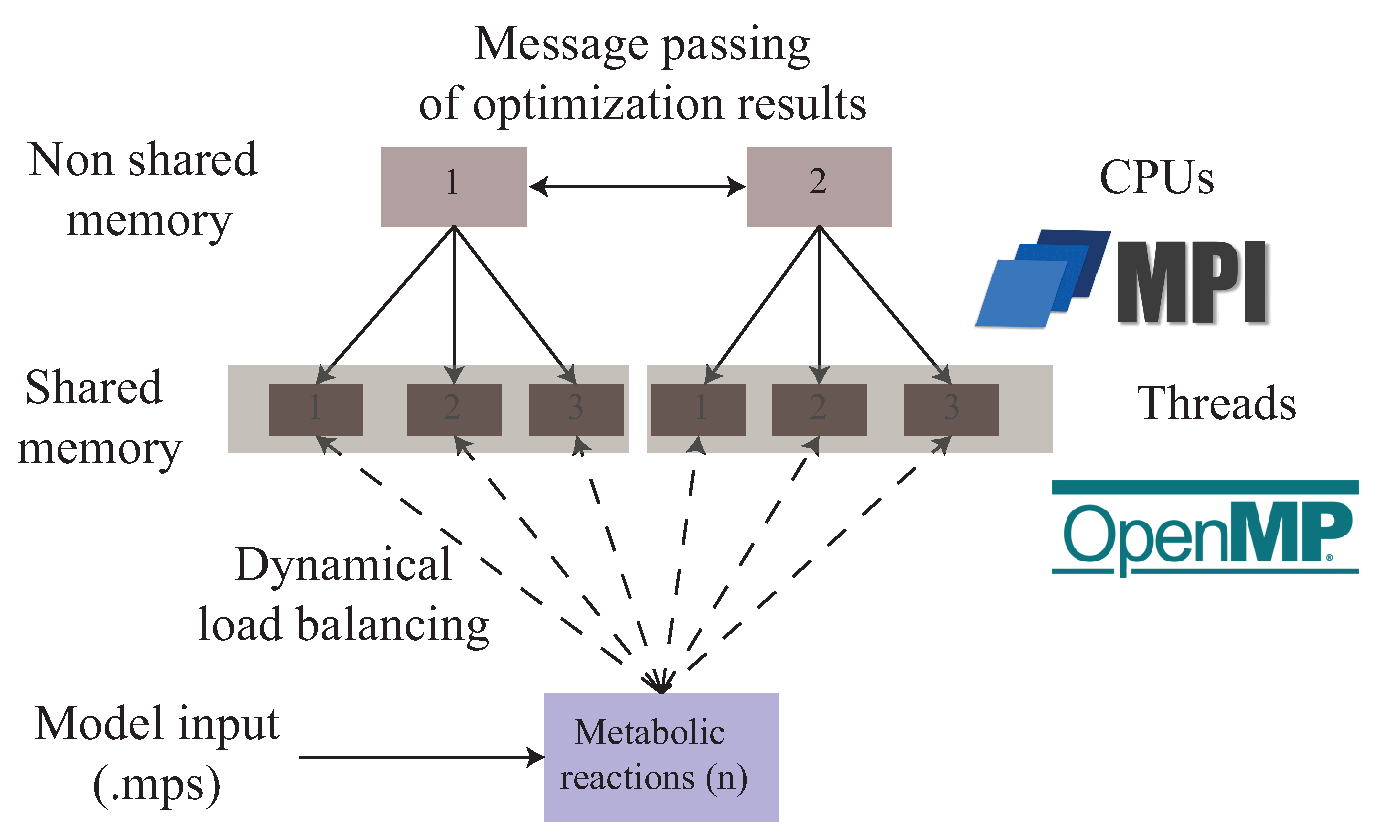
\includegraphics[width=\textwidth,height=\textheight,keepaspectratio]{VFFVA/figures/figure1/scheme.eps}
\caption[Hybrid OpenMP/MPI implementation of FVA.]{Hybrid OpenMP/MPI implementation of FVA ensures two levels of parallelism. The distribution of tasks is implemented following a hierarchical model where MPI manages coarse-graine parallelism in non-shared memory systems and OpenMP processes within each MPI process manage fine-grain parallelism taking advantage of the shared memory to improve performance.}
\label{fig:hybrid.}
\end{figure}
\subsection{Impact on computing small models}
We run VFFVA and FFVA five times on small models i.e., Ecoli\_core, EcoliK12, P\_putida. VFFVA had at least 20 fold speedup (Table \ref{tbl:VFFVAmodelComp}). The main contributing factor was the use of C over MATLAB in all steps of the analysis. In particular, the loading time of MATLAB java machine and the assignment of workers through \texttt{parpool} was much greater than the analysis time itself.\\
The result highlighted the power of C in gaining computing speed, through managing the different low-level aspects of memory allocation and variable declaration.\\
In the analysis of large models, where MATLAB loading time becomes less significant, dynamic load balancing becomes the main driving factor of the gained speedup.\\ 
\begin{table}[h]
\caption[Comparison of run times of FFVA and VFFVA in small models.]{Comparison of run times of FFVA and VFFVA in small models in seconds.}
\begin{center}
    \begin{tabular*}{\textwidth}{l @{\extracolsep{\fill}} llll}
    \hline
    Model & \pbox{2cm}{FFVA \\ mean(std) \\ loading and analysis time} & \pbox{2cm}{VFFVA \\ mean(std) \\ loading and analysis time} & \pbox{1.5cm}{FFVA \\ mean(std) \\ analysis only} \\ \hline
    \multicolumn{4}{c}{2 cores} \\ \hline
    Ecoli\textunderscore core & 19.5(0.5)  & 0.2(0.01) & 0.37(0.1) \\ \hline
	P\_putida & 19.2(0.7) & 0.6(0.02) & 0.81(0.09) \\ \hline    
    EcoliK12 & 20.4(0.6) & 2.2(0.06) & 2.41(0.09)\\ \hline
        \multicolumn{4}{c}{4 cores} \\ \hline
    Ecoli\textunderscore core & 19.6(0.6)  & 0.2(0.005) & 0.32(0.01) \\ \hline
    P\_putida & 19.4(1) &  0.5(0.02) & 0.61(0.01) \\ \hline
    EcoliK12 & 20(0.8) & 1.3(0.04) & 1.64(0.08)\\ \hline
        \multicolumn{4}{c}{8 cores} \\ \hline
    Ecoli\textunderscore core & 19.4(0.5)  & 0.2(0.03) & 0.35(0.05)  \\ \hline
    P\_putida & 19.6(0.7) & 0.4(0.04) & 0.53(0.009) \\ \hline
    EcoliK12 & 20(0.49) & 0.9(0.01) & 1.22(0.08)\\ \hline
        \multicolumn{4}{c}{16 cores} \\ \hline
    Ecoli\textunderscore core &  20.2(0.4) & 0.2(0.008) & 0.41(0.05) \\ \hline
    P\_putida & 19.5(0.4) & 0.4(0.04) & 0.51(0.03) \\ \hline
    EcoliK12 & 22(0.7) & 0.7(0.01) & 0.87(0.03)\\ \hline
        \multicolumn{4}{c}{32 cores} \\ \hline
    Ecoli\textunderscore core & 22.2(0.4)  & 0.3(0.008) & 0.6(0.12)\\ \hline
    P\_putida & 21.5(0.6) &  0.4(0.01) & 0.53(0.004)\\ \hline
    EcoliK12 & 21.5(0.6) & 0.6(0.03) & 0.78(0.04)\\ \hline
    \end{tabular*}
\end{center}
\label{tbl:VFFVAmodelComp}%descriptive label to refer to figure in text
\end{table}
\subsection{Impact on computing large models}
The speedup gained on computing large models (Recon2 and E\_Matrix) reached three folds with VFFVA (Figure \ref{fig:largemodel.}) at 32 threads with Recon 2 (35.17$s$ vs 10.3$s$) and E\_Matrix (44$s$ vs 14.7$s$). In fact, with dynamic load balancing, VFFVA allowed to update the assigned chunks of iterations to every worker dynamically, which guarantees an equal distribution of the load. In this case, the workers that get fast-solving LPs, will get a larger number of iterations assigned, while those that get ill-conditioned LPs and require more time to solve them, will get fewer LPs in total, in such way that all workers synchronize at the same time to reduce the results. Particularly, the speedup achieved with VFFVA increased with the size of the models and the number of threads (Figure \ref{fig:largemodel.}-E\textunderscore Matrix). 
Finally, we further explored the different load balancing startegies (static, guided and dynamic) with two of the largest models (E\textsubscript{c}\textunderscore Matrix and Harvey).
\begin{figure}[!htp]
\centering
\includegraphics[width=\textwidth,height=\textheight,keepaspectratio]{VFFVA/figures/figure2/largemodels.eps}
\caption[Run times of Recon2 and E\textunderscore Matrix model.]{Run times of Recon2 and E\_Matrix model using FFVA and VFFVA on 2,4,8,16, and 32 threads. The guided schedule was used in the benchmarking.}
\label{fig:largemodel.}
\end{figure}
\subsection{Load management}
Load management describes the different approaches to assign iterations to the workers. It can be static, where an even number of iterations is assigned to each worker. Guided schedule refers to dividing the iterations in chunks of size $n/workers$ initially and $remaining\textunderscore{iterations}/workers$ afterwards. The difference with static lies in the dynamic assignment of chunks, in a way that fast workers can process more iteration blocks. Finally, dynamic schedule is very similar to guided except that chunk size is given by the user, which allows a greater flexibility. In the following section, we will compare the load balancing strategies of E\textsubscript{c}\textunderscore Matrix and Harvey models.\\
\begin{figure}[!htp]
\centering
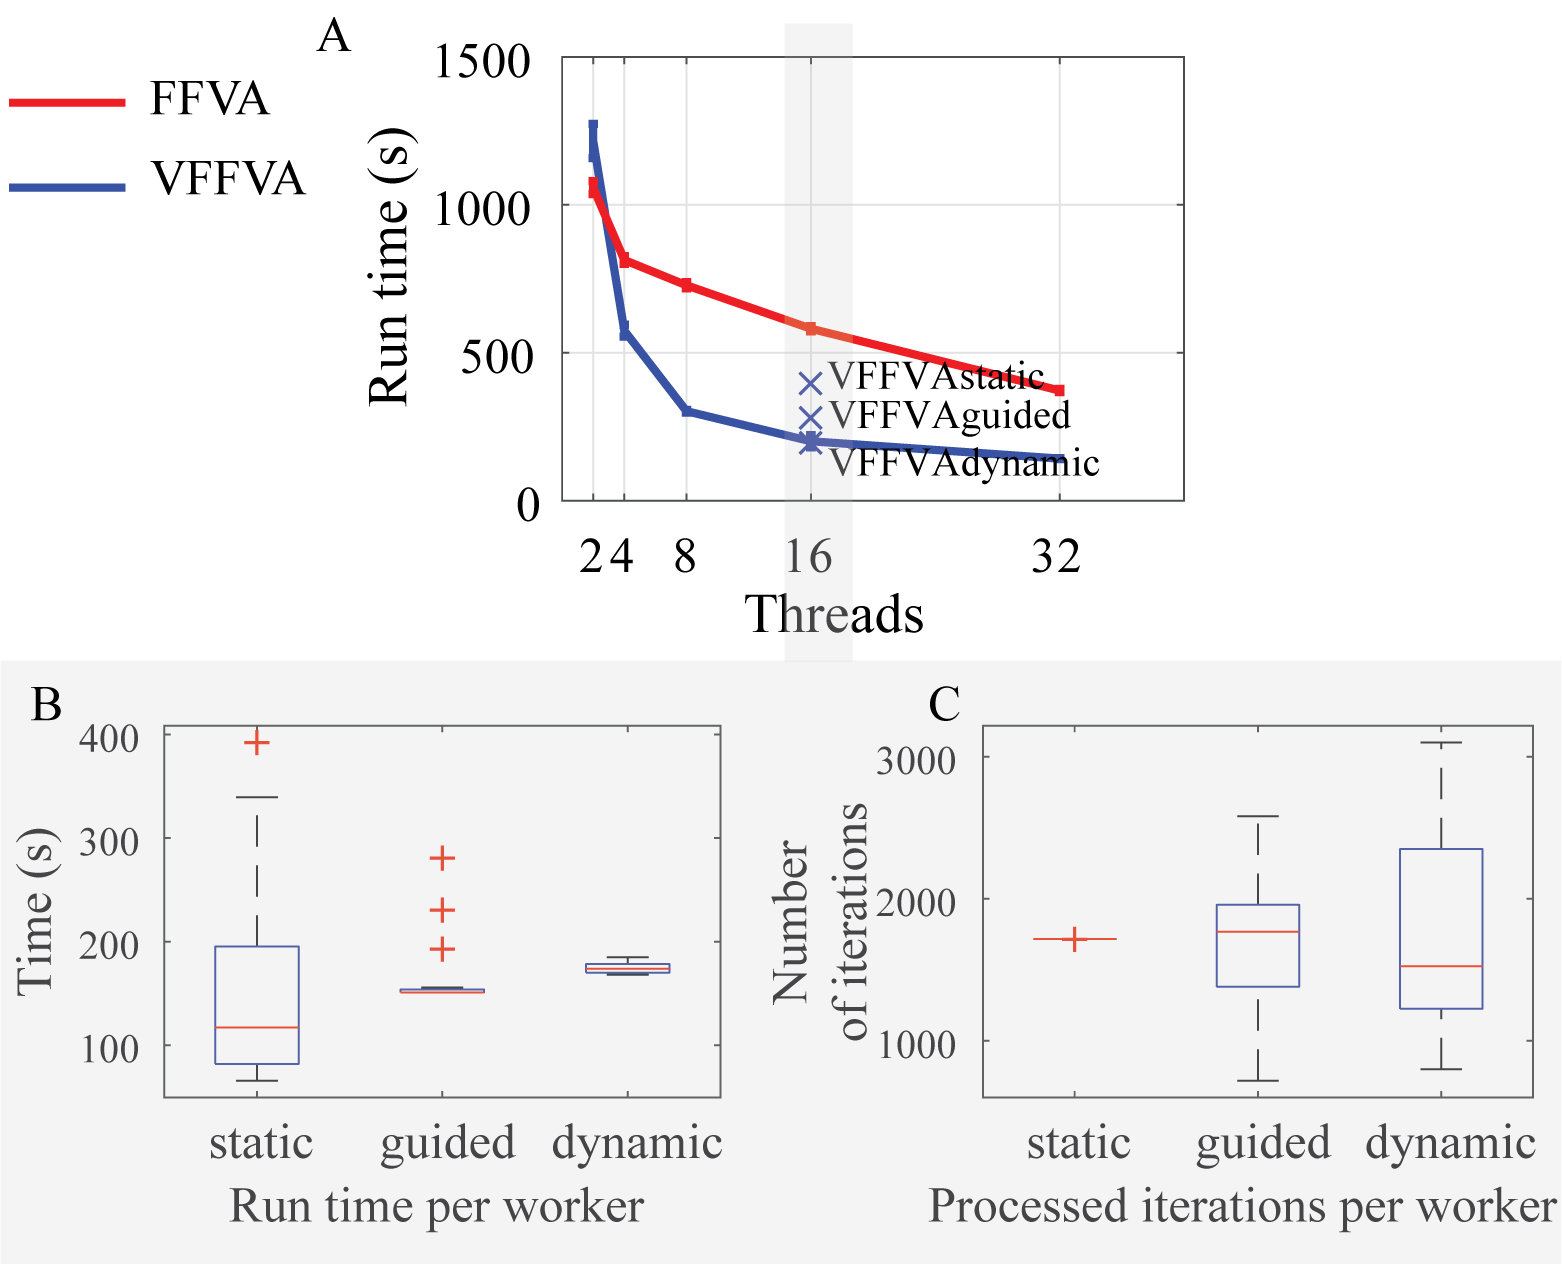
\includegraphics[width=\textwidth,height=\textheight,keepaspectratio]{VFFVA/figures/figure3/schedule.png}
\caption[Run times of E\textsubscript{c}\textunderscore Matrix model.]{Run times of E\textsubscript{c}\textunderscore Matrix model. A-Run times of E\textsubscript{c}\textunderscore Matrix model at 2,4,8,16, and 32 threads using FFVA and VFFVA. B-Run time per worker in the static, guided, and dynamic schedule using 16 threads. C-The number of iterations processed per worker in the static, guided, and dynamic schedule using 16 threads.}
\label{fig:static.}
\end{figure}
\subsubsection{Static schedule}
Using static schedule, VFFVA assigned an equal number of iterations to every worker. With 16 threads, the number of iterations per worker equalled 1715 and 1716 (Figure \ref{fig:static.}-C). Expectedly, the run time varied widely between workers (Figure \ref{fig:static.}-B) and resulted in a final time of 393$s$.
\subsubsection{Guided schedule}
With guided schedule (Figure \ref{fig:static.}-A), the highest speedup (2.9) was achieved with 16 threads (Figure \ref{fig:static.}-B). The run time per worker was quite comparable and the iterations processed varied between 719 and 2581. The final run time was 281$s$.
\subsubsection{Dynamic schedule}
Using a dynamic load balancing with a chunk size of 50 resulted in similar results to the guided schedule. The final run time equalled 197$s$, while FFVA took 581$s$. An optimal chunk size has to be small enough to ensure a frequent update on the workers load, and big enough to take advantage of the solution basis reuse in every worker. At a chunk size of 1 i.e. each worker is assigned 1 iteration at a time, the final solution time equalled 272$s$. The reason being that if the worker is updated quite often with new pieces of iterations, then it looses the stored solution basis of the previous problem and has to solve from scratch.\\ 
\begin{figure}[!htp]
\centering
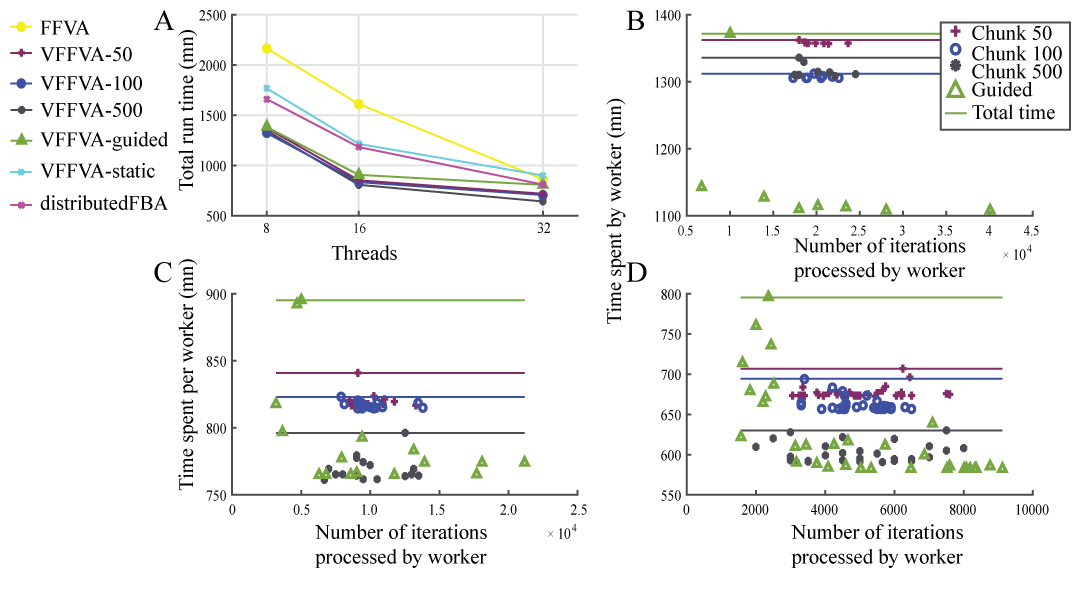
\includegraphics[width=\textwidth,height=\textheight,keepaspectratio]{VFFVA/figures/figure4/harvey.png}
\caption[Run times per worker of Harvey model.]{Run times per worker of Harvey model. A- Total run time of the different load balancing schedules at 8, 16, and 32 threads. B-Run time per worker as a function of the number of iterations processed using the guided schedule and the dynamic schedule with chunk size of 50, 100, and 500 with 8 threads, C-16 threads, and D-32 threads.}
\label{fig:harvey.}
\end{figure}
Similarly, Harvey model \cite{thiele2018metabolism} (Figure \ref{fig:harvey.}-A) had a 2-fold speedup with 16 threads using a chunk size of 50 (806 mn) compared to FFVA (1611 mn). The run times with guided schedule (905 mn), dynamic schedule with chunk size 100 (850 mn) and chunk size 500 (851 mn) were less efficient due to the slower update rate leading to a variable analysis time per worker (Figure \ref{fig:harvey.}-B,C,D). VFFVA on 8 threads (1323 mn with chunk size 50) proved comparable to FFVA (1214 mn) and distributedFBA (1182 mn) on 16 threads, thereby saving computational resources and time. 
\subsection{Impact on memory usage}
In MATLAB, the execution of $j$ parallel jobs implies launching $j$ instances of MATLAB. On average, one instance needs 2 Gb. In parallel setting, the memory requirements are at minimum $2j$ Gb, which can limit the execution of highly parallel jobs. In the Julia-based distributedFBA, the overall memory requirement exceeded 15 Gb at 32 cores. VFFVA requires only the memory necessary to load $j$ instances of the input model, which corresponds to the MPI processes as the OpenMP threads save additional memory through sharing one instance of the model. The differences between the FFVA and VFFVA get more pronounced as the number of threads increases (Figure \ref{fig:memory.}) i.e., 13.5 fold at 8 threads, 14.2 fold at 16 threads, and 14.7 fold at 32 threads.\\
Finally, VFFVA outran FFVA and distributedFBA both on execution time and memory requirements (Table \ref{tbl:VFFVAalgocomp}). The advantage becomes important with larger models and higher number of threads, which makes VFFVA particularly suited for analysing the exponentially-growing-in-size metabolic models in HPC setting.
\begin{table}[h]
\caption[Comparative summary of the methods' features.]{Comparative summary of the methods' features.}
\begin{center}
    \begin{tabular*}{\textwidth}{l @{\extracolsep{\fill}} lllll}
    \hline
    Feature & VFFVA & distributedFBA & FFVA & FVA \\ \hline
    Speed & ++++ & +++ & ++ & + \\ \hline
    Memory & +++ & ++ & + & + \\ \hline 
    Load balancing & dynamic & static & static & static \\ \hline 
    \end{tabular*}
\end{center}
\label{tbl:VFFVAalgocomp}%descriptive label to refer to figure in text
\end{table}
\begin{figure}[!htp]
\centering
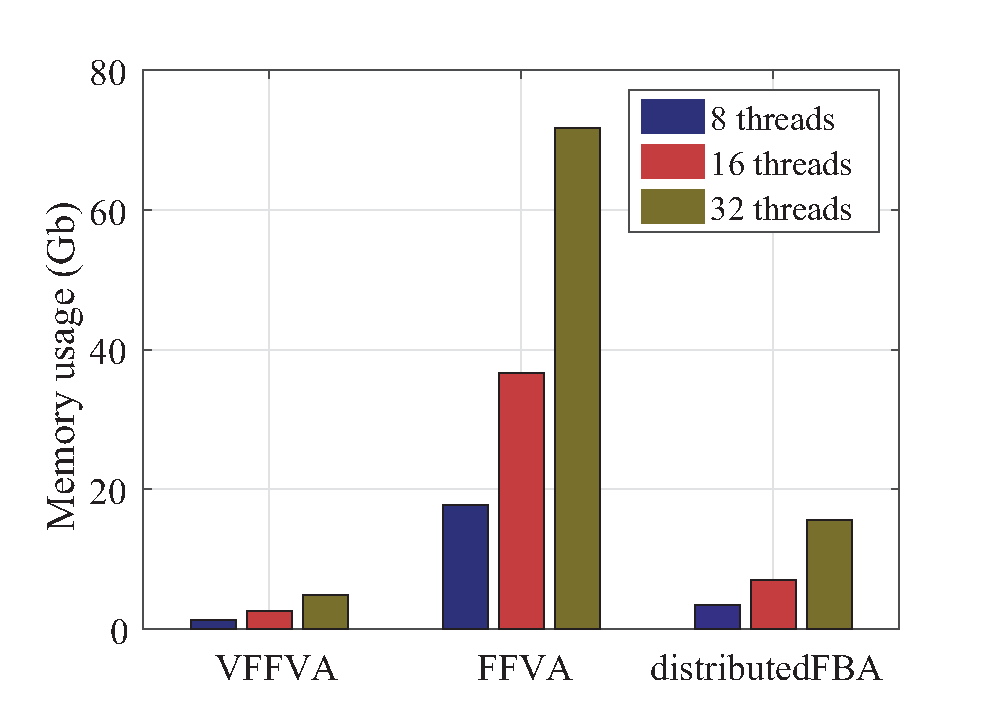
\includegraphics[width=\textwidth,height=\textheight,keepaspectratio]{VFFVA/figures/figure5/memoryUsage.eps}
\caption[Physical memory usage at 8, 16, and 32 threads.]{Physical memory usage at 8, 16, and 32 threads using FFVA, VFFVA, and distributedFBA.}
\label{fig:memory.}
\end{figure}
\subsection{Creation of warmup points for sampling}
We compared the generation of 30,000 warmup points using the COBRA toolbox function createWarmup\textsubscript{MATLAB}  and a dynamically load-balanced C implementation createWarmup\textsubscript{VF} on a set of models (Table \ref{tbl:VFwarmup}). Since the COBRA toolbox implementation does not support parallelism, we run it on a single core and divided the run time by the number of cores to obtain an optimistic approximation of the parallel run times. The speedup achieved varied between four up to a factor of 100 in the different models (Table \ref{tbl:VFwarmup}). Similarly to FFVA \cite{gudmundsson2010computationally}, the main factor for the speedup was the C implementation that allowed the reuse of the LP object in every iteration and save presolve time. Equally, the dynamic load balancing between workers ensured a fast convergence time.\\
Taken together, the dynamic load balancing strategy allows the efficient parallel solving of metabolic models through accelerating the computation of FVA and the fast preprocessing of sampling points thereby enabling the modeller to tackle large-scale metabolic models.
\begin{table}[!htp]
\caption[Generation of sampling warmup points using dynamic load balancing.]{Generation of sampling warmup points using dynamic load balancing.}
\begin{center}
    \begin{tabular*}{\textwidth}{l @{\extracolsep{\fill}} llllllll}
    \hline
    Model &createWarmup\textsubscript{MATLAB} & \multicolumn{6}{c}{createWarmup\textsubscript{VF}}\\ \hline
    Cores&1&1&2&4&8&16&32 \\ \hline
    Ecoli\textunderscore core & 149 & 2.8 &1.8 & 0.8 & 0.7 & 0.5 & 0.5 \\ \hline
	P\_putida & 385& 12.5 & 13 & 8 & 4 & 2 & 2 \\ \hline    
    EcoliK12 & 801& 49 & 43 & 23 & 10.4 & 9.5 & 9.1 \\ \hline
    Recon2 & 11346& 288 & 186  & 30 & 32 & 24 & 21 \\ \hline
    E\_Matrix & NA\textsuperscript{*}& 602 & 508 & 130 & 52 & 43 & 43 \\ \hline
    E\textsubscript{c}\_Matrix & NA\textsuperscript{*} & 5275 & 4986 & 924 & 224 & 118  & 117  \\ \hline
    \end{tabular*}
\end{center}
\caption*{\textsuperscript{*} The generation of warmup points of E\_Matrix and E\textsubscript{c}\_Matrix models did not converge after 20000 $s$. The creation of warmup points can vary widely between runs as it involves the generation of a random $c$ vector in the linear program. The runs were repeated three times and the average was reported. }
\label{tbl:VFwarmup}%descriptive label to refer to figure in text
\end{table}
\section*{Acknowledgements}
The authors would like to acknowledge fastFVA authors for publicly sharing their code, IBM for providing a free academic version of ILOG CPLEX as well as Valentin Plugaru and Dr. Laurent Heirendt at the University of Luxembourg, for useful comments and guidance. The experiments presented in this paper were partly carried out
using the HPC facilities of the University of Luxembourg~\cite{VBCG_HPCS14} 
{\small -- see \url{http://hpc.uni.lu}}.%Path to chapter

\chapter{Pan-organ model integration of regulatory and metabolic processes in type 1 diabetes.}
\label{ch:chapter5}
\chaptermark{Whole-body dynamic model}%Short description for page header
{\setstretch{1.0} \textit{Manuscript in preparation.} \par}%Paper reference, note, other. Can remove. Single line space.
\section*{Abstract}
{\setstretch{1.0}  
Type 1 diabetes is a systemic disease triggered by a local autoimmune inflammatory reaction in the insulin-producing cells. The disruption of the glucose-insulin-glucagon system induces organ-wide, long-term effects on glycolytic and non-glycolytic processes. Mathematical modeling of the whole-body regulatory bihormonal system helped identifying intervention points to ensure a better control of type 1 diabetes mellitus. We present a whole-body model, developed using an integrative modeling framework termed CRONICS, linking regulation and metabolism in an organ-resolved manner. The developed framework allowed to correctly predict disrupted metabolic processes in type 1 diabetes in relation to the symptoms, highlighted common pathophysiological processes with neurodegenerative disorders and suggested calcium channel blockers as potential adjuvants for diabetes control. Additionally, the model predicted an insulin-dependent rewiring of inter-organ crosstalk. Moreover, it allowed to assess the impact of inter- and intra-individual variability to insulin treatment and their implications on clinical outcome. In particular, GLUT-4 is suggested as a potential pharmacogenomics regulator of intra-individual insulin efficacy. The organ-resolved, dynamic model opens the way to better understand human pathology and the model-based design of precise allopathic strategies.
\par}%single line space

\newpage
\begin{figure}[!htp]
\centering
	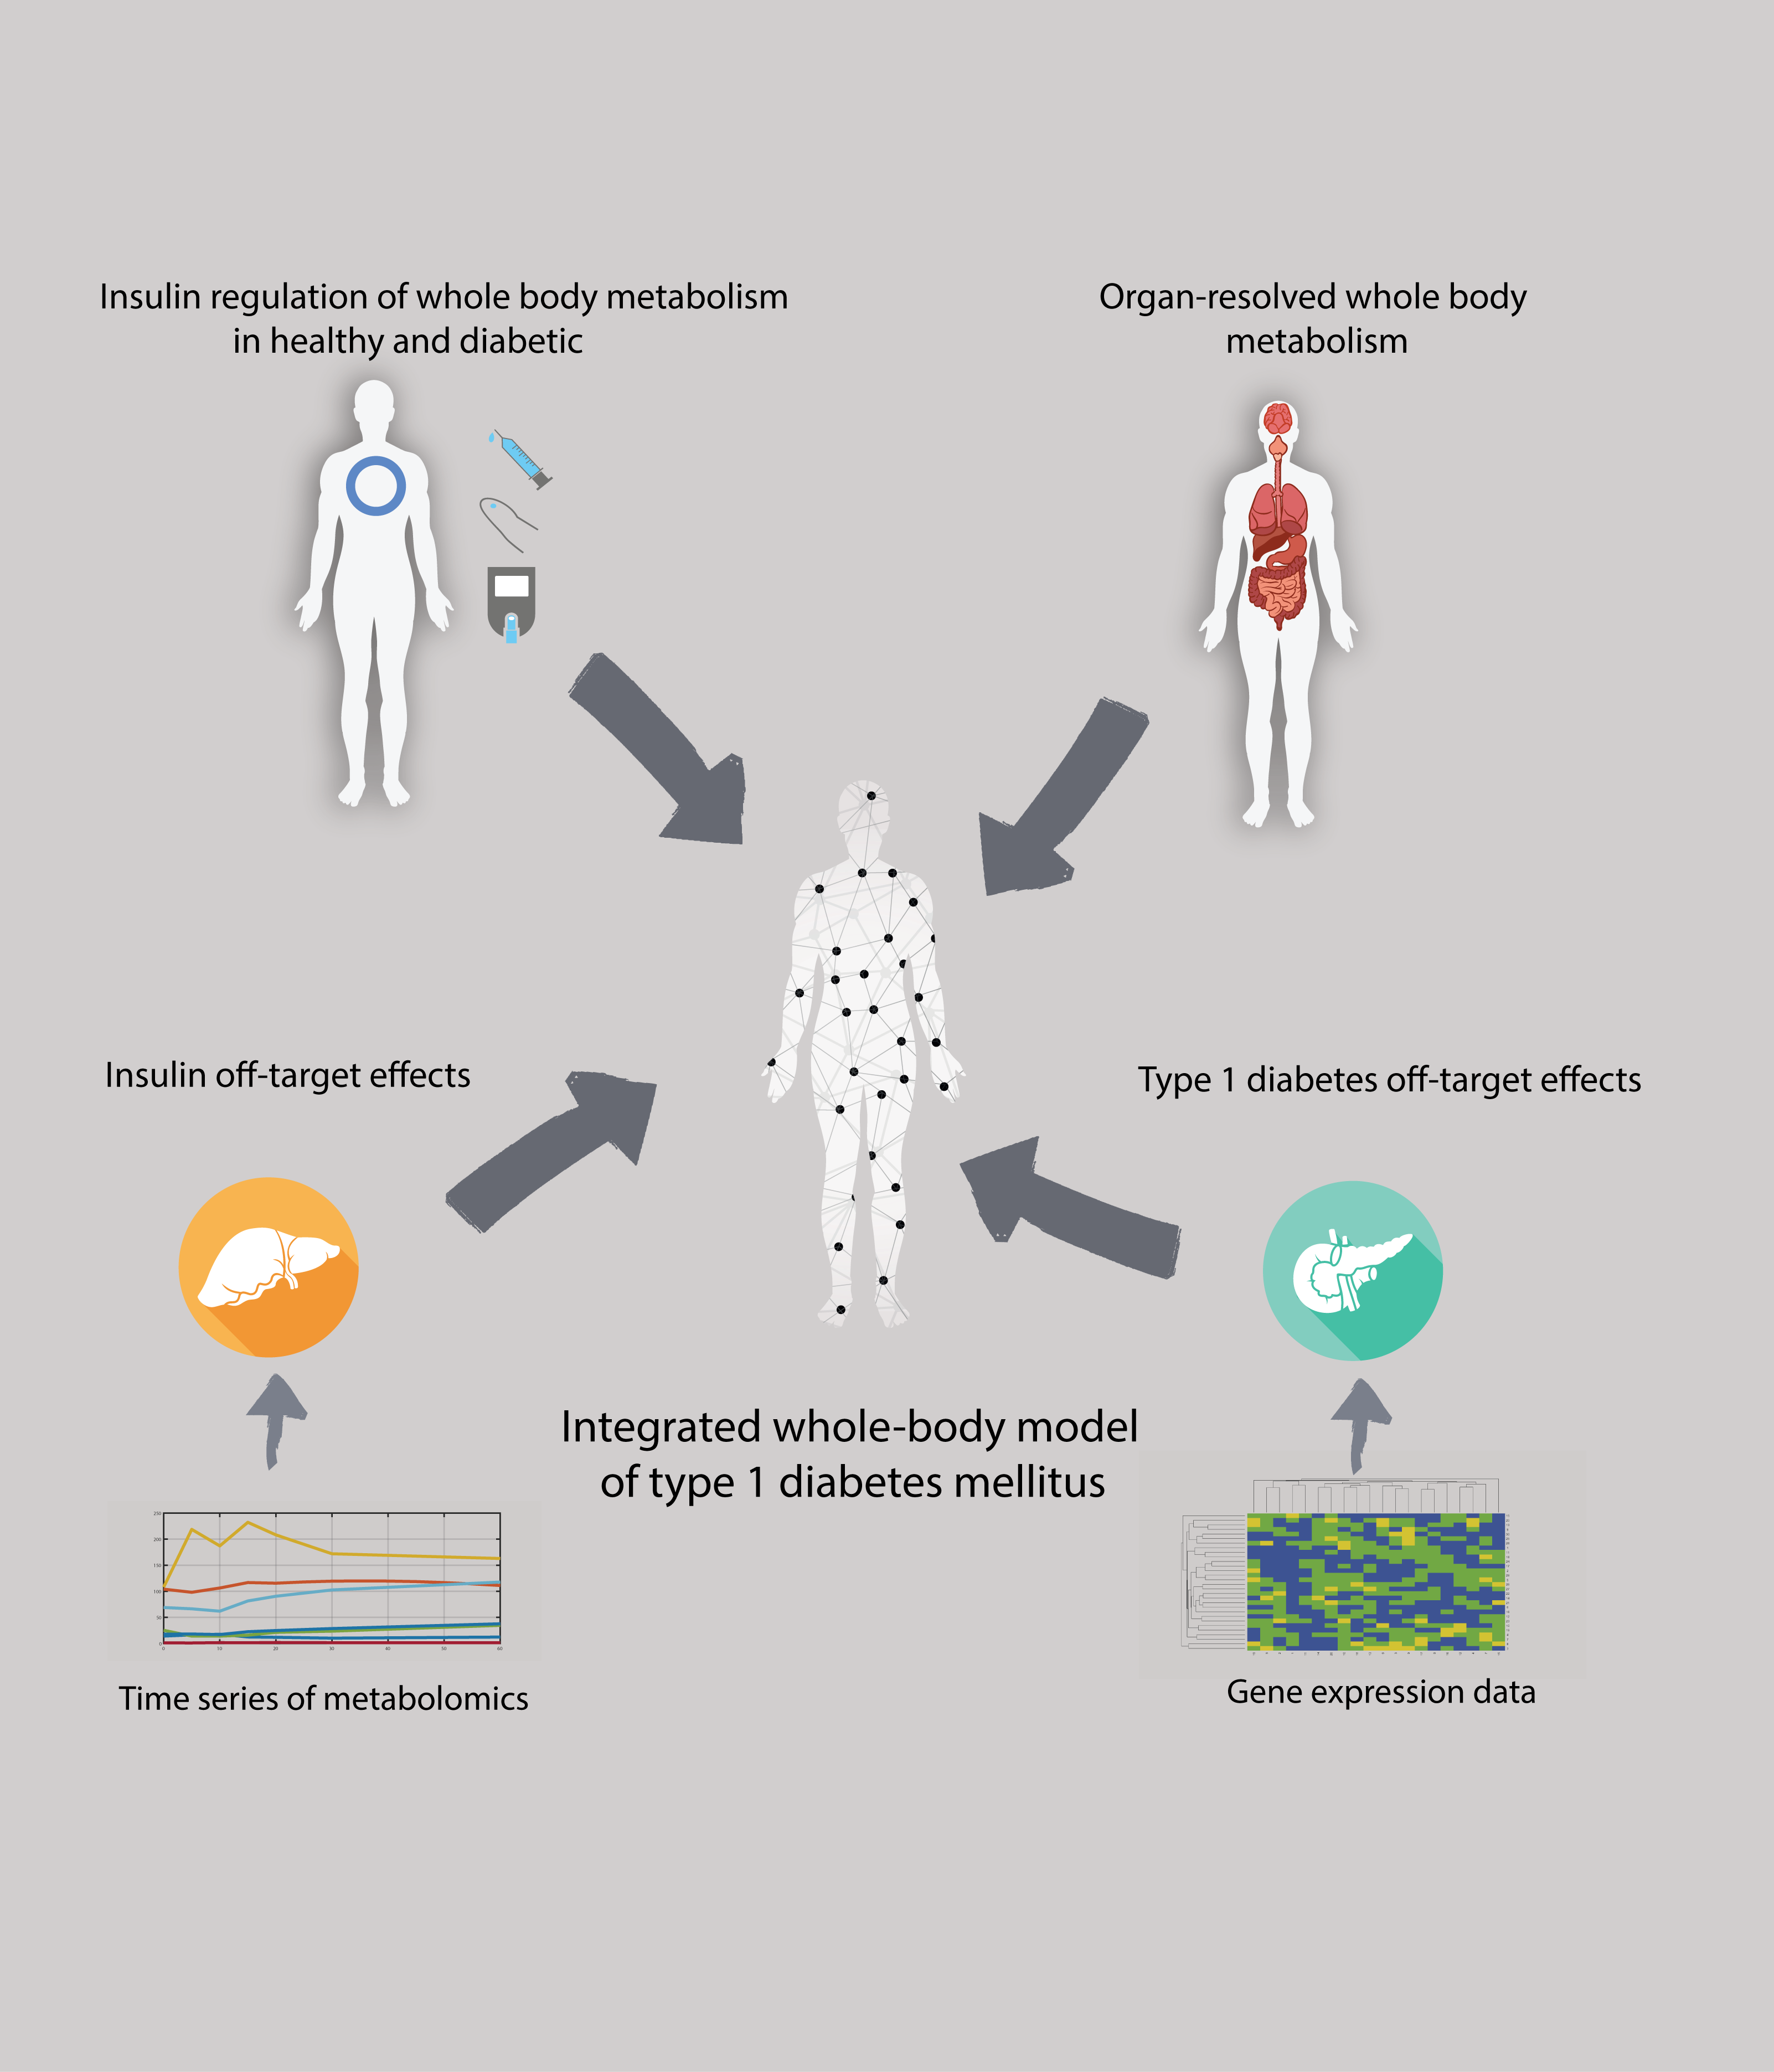
\includegraphics[width=\textwidth,height=\textheight,keepaspectratio]{GIM/studySummary.png}%Figure from images\Figure1.png
	\caption[Study summary of whole-body dynamic metabolism.]{Study summary of whole-body dynamic metabolism in type 1 diabetes. A whole-body dynamic model of type 1 diabetes integrates a whole-body, organ-resolved metabolic model (Harvey), with a whole-body dynamic model of the glucose-insulin-glucagon system (GIM), type 1 diabetes gene expression in the pancreas, and insulin-induced metabolite concentration time-course. The model captured the state-of-the-art knowledge about type 1 diabetes and gave insights into within and between-patient variability to insulin response.}
	\label{fig:GIMSummary}
\end{figure}

\newpage
\section{Introduction}
Type 1 diabetes (T1D) mellitus is a systemic disease triggered by the destruction of insulin-producing pancreatic beta cells \cite{maahs2010epidemiology}. The World Health Organization estimated the incidence of up to 36.8 new cases in 100,000 persons per year with an increase of 2 to 5\% worldwide \cite{maahs2010epidemiology}. It remains the most prevalent type of diabetes in children and has cumbersome lifelong effects \cite{maahs2010epidemiology}. The disease affects primarily the production of insulin causing acute metabolic complications and coronary artery disease, resulting in high early mortality rates \cite{orchard2006type}. Additionally, the misdiagnosis of T1D in adults is a recently acknowledged issue \cite{thomas2017frequency}, as the delay in implementing the insulinotherapy can further exacerbate the disease symptoms.
The systemic mechanism of action of insulin induces the whole-body semiology of T1D. The symptoms include several glucose dependent metabolic processes such as micro- and macroangiopathy, diabetic retinopathy, and nephropathy, as well as fatty acids related implications like atherosclerosis and cardiovascular disease \cite{american2014diagnosis}. Supplementing patients with exogenous insulin remains the gold standard treatment of type 1 diabetes. Although being  very efficient in preventing biochemical alterations, insulin has a high within and between subject variability that can induce adverse reactions ranging from hypoglycemia to uncontrolled diabetes; effects that can hamper the treatment compliance \cite{heinemann2002variability}.\\
The wealth of data in type 1 diabetes helped the development of whole-body mathematical models of insulin action and disease progression, notably the ODE-based glucose insulin model (GIM) \cite{schaller2013generic}. GIM includes fine-grained details of tissue-based insulin and glucagon action in relation to glucose dynamics such as insulin-dependent receptor synthesis and the gastrointestinal hormonal regulation of glucose levels. It could also reproduce the outcome of differential diagnosis tolerance tests on type 1 diabetic patients. The model extensively described the bihormonal regulatory events yet modeling of metabolism remained limited to the first step of glycolytic pathways.\\
Therefore, the systematic analysis of disrupted metabolic processes beyond glycolysis in type 1 diabetes needs extended approaches. To better capture metabolism, we used the constraint-based reconstruction of the organ-resolved whole-body human metabolic network (Harvey) \cite{thiele2018metabolism}. Harvey includes the tissue-specific metabolic pathways of 20 organs, six sex organs, and six blood cells enabling thereby the modelling of carbohydrate disorders and the study of their impact on non-glycolytic pathways. Therefore, the whole-body model provides a complete picture of organ-resolved human metabolism, yet addressing disease dynamics and the patient's response to insulin requires the modeling of both the metabolic pathways as well as non-metabolic processes including insulin receptor binding, transduction of signal, and internalisation of receptors. Recently, multi-scale, multi-algorithm, whole-organism dynamic models in biology \cite{oyaas2017genome} have seen a surge in complexity, addressing mostly microbiology \cite{karr2012whole,covert2008integrating}, plant physiology \cite{grafahrend2013multiscale}, and also human physiology and xenobiotic metabolism \cite{krauss2012integrating}. 
Accordingly, we coupled the organ-resolved whole-body model (Harvey) with the dynamic glucose insulin ODE-based model (GIM). The multiscale model (dHarvey) allowed to represent type 1 diabetes through both glycolytic target effects and off-target effects that were mapped onto the model using gene expression data. Particularly, the effects of insulin were added through including an additional dynamical model representing its impact on liver metabolism. The model including the target and off-target effects of both type 1 diabetes and insulin, allowed to i) quantify disrupted metabolic process in type 1 diabetes in relation the disease symptomatology, ii) assess insulin non-glycolytic effects, and iii) shed new light on mechanisms underlying inter and intra-individual variability of insulin effects. The hybrid model provides a kernel for the organ-specific integration of biological data and paves the way for predictive human physiology.

\section{Methods}
\subsection{Coupling the dynamical model and the constraint-based model} \label{meth1}
Determining the metabolic reaction flux in the constraint-based model (Harvey) requires solving the usual liner program:
\begin{alignat*}{2}
  & \text{max: } &  & c^{T}v_{H}\\
  & \text{subject to: } &  &  
                \begin{aligned}[t] \\
                & Sv_{H} = b_{H} \\
                & v_{min} \leq v_{H}  \leq  v_{max}
                \end{aligned}
\end{alignat*}
,with $c$ the objective coefficient vector, $S_{m,n}$ the stoichiometric matrix of $m$ metabolites and $n$ reactions, $v_{H}$ the flux vector bounded by $v_{min}$ the lower bound vector and $v_{max}$ the upper bound  vector. When $b_{H}=0_{m}$, the problem is constrained by $Sv=0$, also referred to as Flux Balance Analysis (FBA) \cite{orth2010flux}.\\
Points of intersection between the dynamical model (GIM) and the constraint-based model (Harvey) included metabolites and reactions. There were four classes of correspondences (Figure \ref{fig:GIM0}) that resulted in different implementations of the coupling constraints (Text \ref{GIM:sp1}). Let us first consider the concentrations of a given metabolite modelled in GIM (G) by the following ODE:
\begin{equation*}
\frac{dC_{G,n}}{dt}=X_{G,prod}-X_{G,elim}
\end{equation*}
,with $X_{prod}$ and $X_{elim}$ are reaction fluxes respectively producing and eliminating the metabolite $n$ through first order processes.\\
Case 1: If one reaction in the dynamical model corresponded to one reaction in the metabolic model, the constraints for one time step were subjected as follows:
\begin{equation*}
v_{H,i}=X_{G,j}
\end{equation*}
,with $t$ as the time, $v$ the flux vector, $i$ the index of the reaction in the Harvey model ($H$), and $j$ the index of the reaction in the GIM model such that reactions $i$ and $j$ perform the same metabolic function, e.g., liver hexokinase reaction.\\ 
Case 2: When a metabolite is represented in both models, the sum of its anabolic and catabolic fluxes in Harvey is constrained by its change-of-concentration in GIM, also referred to as metabolite pooling fluxes \cite{covert2008integrating}. The constraints are formulated as the following:
\begin{equation*}
b_{H,m}=\frac{dC_{G,n}}{dt}
\end{equation*}
,with $m$ referring to the metabolite in Harvey, $n$ the metabolite in GIM, $C_n$ the concentration of $n$, and $b$ the vector of metabolite change-of-concentration in Harvey. \\
Case 3: The third case corresponds to one reaction in GIM being represented by more than one reaction in Harvey. Typically, they correspond to reactions catalyzed by cofactor-dependent enzymes such as hexokinase with ATP and ADP as cofactors. The reaction pooling fluxes are then subjected as follows:
\begin{equation*}
\sum_{i=1}^{k} v_{H,i}=X_{G,l}
\end{equation*}
,with $v_1$ to $v_k$ are the reactions in Harvey corresponding to reaction $l$ in GIM. \\
Case 4: In the case when one metabolite in GIM corresponds to more than one metabolite in Harvey, such as blood cells glucose in GIM corresponding to glucose in red blood cells, monocytes, natural killer cells, B cells, platelets, and CD4 T cells in the metabolic model, the constraints are formulated as follows:
\begin{equation*}
\sum_{i} (v_{H,a(i)}+v_{H,c(i)})=\frac{dC_{G,j}}{dt}
\end{equation*}
,with $v_a$ the anabolic fluxes, $v_c$ the catabolic fluxes, $i$ the index of the different metabolites in Harvey corresponding to metabolite $j$ in GIM. 
After subjecting the constraints, the steady-state was assumed in the chosen time step for the non-overlapping metabolites in both models, such as amino acids. The constraints then translates to the following:
\begin{equation*}
S.v_{H}=b_{H}
\end{equation*}
,with $S$ the stoichiometric matrix of Harvey, $v$ the flux vector, and $b$ the metabolite concentration change, that equalled zero for steady-state metabolite and non-zero for metabolites falling under case 2. When the applied constraints rendered the linear program infeasible, the lower and upper bounds were relaxed minimally in both the amplitude of relaxation and the cardinal of the reactions to be relaxed (Text \ref{GIM:sp2}).\\
The simulation of tolerance tests, and the assessment of the inter and intra-individual variability to insulin response were performed using dHarvey with specific model parameters. The tolerance tests parameters were as reported in the GIM model \cite{schaller2013generic} (Table \ref{GIM:tbls3}), which includes trials in healthy and T1D patients for intravenous insulin tolerance test (IVITT), intravenous glucose tolerance test (IVGTT), baseline glucose concentration (Noinf), subcutaneous insulin bolus (SCIB), subcutaneous insulin infusion (SCII), solid meal (WB-Solid), oral liquid glucose solution (WB-Liquid). The parameters of the GIM model were reportedly \cite{schaller2013generic} identified using tolerance tests trial data \cite{sorensen1985physiologic,regittnig1999plasma} and bihormonal closed-loop experiments \cite{el2010bihormonal}. Harvey was simulated using exchange reactions corresponding to standard European diet \cite{sahoo2013predicting}.
\subsection{Comparison of the predictive capabilities of the different models}
In order to compare the predictive capabilities of Harvey, GIM, and dHarvey, we simulated the intravenous glucose tolerance test (IVGTT). GIM includes a parameter set for simulating IVGTT (Table \ref{GIM:tbls3}) and glucose concentrations were obtained through integrating the ODEs.\\
Glucose concentrations in Harvey alone were obtained through dFBA. Briefly, the initial amount of glucose is set as availability constraints and decreases in every time step after subtracting the consumed glucose fluxes obtained through solving the linear program \cite{mahadevan2002dynamic}. The maximum rate-of-change of glucose was set to the intravenously injected amount in the $b$ vector, the problem translates then to the following:
\begin{alignat*}{2}
  & \text{max: } &  & c^{T}v\\
  & \text{subject to: } &  &  
                \begin{aligned}[t] \\
                & Sv \leq b \\
                & v_{min} \leq v  \leq  v_{max}
                \end{aligned}
\end{alignat*}
dHarvey not only reproduced the glucose time series of GIM but also could predict the time course of ATP, which is not present in GIM. The simulation was done through setting ATP demand reaction in each time step as the objective function as the following:
\begin{alignat*}{2}
  & \text{max: } &  & c^{T}v\\
  & \text{subject to: } &  &  
                \begin{aligned}[t] \\
                & Sv=0 \\
                & v_{min} \leq v  \leq  v_{max}
                \end{aligned}
\end{alignat*}
, with $c$ the vector of objective function coefficients and $v_{min}$,$v_{max}$ respectively, the minimum and maximum flux going through the reaction. The $c$ vector entry corresponding to the indices of reactions corresponding to ATP demand in every organ were set to one. Then, the baseline value of ATP demand reaction flux, calculated at the initial simulation time, was subtracted from the obtained value. A cumulative sum of the resulting fluxes allowed to get the theoretical time course of ATP in a given tissue. 
\subsection{Modeling T1D off-target effects in the pancreas}
We considered T1D as the combination of target and off-target effects. The target effects are directly related to the decrease of insulin secretion and the increase of glucose levels and the off-target effects are represented in the underlying chronic inflammation that triggers the disease. To model target effects, we constructed dHarvey healthy and T1D models that were obtained through coupling Harvey with healthy and T1D GIM models. Moreover, consensus gene expression data \cite{planas2010gene} of pancreas biopsies of type 1 diabetic patients obtained through whole genome sequencing of four patients after five days, nine months, five years, and ten years post-diagnosis were used to further constrain the dHarvey diabetic model and to capture the chronic inflammation in the pancreas leading to the development of T1D. Differentially expressed genes were mapped on the metabolic model in order to represent the off-target effects of the disease. Among the list of 475 differentially expressed genes, only the metabolic genes present in Harvey were kept for further analysis, corresponding to 24 genes (Table \ref{GIM:tbls1}). 
Consequently the bounds in the linear program of dHarvey T1D model, were modified in the reactions corresponding to every gene such that:
\begin{gather*}
v_{min(i)}^t=v_{min(i)}^h*fc \\
v_{max(i)}^t=v_{max(i)}^h*fc \\
v_{min(i)}^t<v_i^t<v_{max(i)}^t
\end{gather*}
, with $fc$ the gene expression fold change between control and disease of the gene encoding reaction $i$, $v_{min(i)}^h$  the minimum reaction flux corresponding to reaction $i$ in the healthy model, and $v_{max(i)}^h$ the maximum reaction flux of the healthy model as identified by flux variability analysis. $v_{min(i)}^t$ and $v_{max(i)}^t$ are the new lower and upper flux bound computed in dHarvey type 1 diabetic models. Gene expression allowed to constrain a total of 80 reactions in the pancreas (Table \ref{GIM:tbls2}).
\subsection{Modeling insulin off-target effects in the liver}
Similarly to T1D, we considered insulin to induce target and off-target effects. The target effects of insulin is the reduction of glucose levels, and the off-target effects are the various physiological processes involving insulin such as the regulation of glycolysis. The off-target effects of insulin in the liver were modelled through coupling an additional ODE model to the dHarvey model. The model \cite{yugi2014reconstruction} represented the metabolic effects of insulin on glycolytic fluxes during one hour. The amounts of eight metabolites \textit{in vitro} (fructose-6-phosphate, fructose-1,6-diphosphate, phosphoenolpyruvate, isocitrate, 2-oxoglutarate, malate, frucotse-2,6-biphosphate, and citrate) were scaled to amounts (mmol) \textit{in vivo} as following: 
\begin{equation*}
A_{invivo}=C_{invitro}*V_{hep}*HPGL*V_l
\end{equation*} 
,where $V_{hep}$ is the hepatocyte volume, $HPGL$ is the hepatocellularity, $C_{invitro}$ is the concentration of the metabolites \textit{in vitro} and $V_l$ the liver volume.
The values of the parameters were set as following \cite{heinemann1999standard}:
\begin{gather*}
V_{hep}=3,4.10^{-9} \quad cm^3 \\
HPGL=86.\frac{10^6 cells}{gram \, of \, liver}\\
V_l=322.6 \quad gram
\end{gather*}
The constraints were applied by setting the metabolites rate-of-change in the insulin dynamical model equal to the corresponding $b$ vector value in Harvey.
\subsection{Simulation of inter-individual variability to insulin response}
In order to assess the between subject variability of glucose dynamics after a bolus of insulin (Table \ref{GIM:tbls3}), the identified differential parameters \cite{schaller2013generic} (Table \ref{GIM:tbl1}) between type 1 diabetes and healthy GIM models were randomly varied within 2-fold interval to reproduce the observed 25-35\% of variability in a patient population \cite{heinemann2002variability} as computed by $\frac{std(AUC)}{mean(AUC)}$, where $AUC$ refers to the area under the curve of peripheral glucose concentrations per patient. The parameters were randomly increased or decreased for a synthetic group of 30 patients and the coupling between the newly obtained GIM models and Harvey was performed as described previously.  
\subsection{CRONICS, the simulation algorithm}
The simulations were done following two main methods: direct and indirect coupling \cite{covert2008integrating,krauss2012integrating}. Indirect coupling was used to dynamically constrain Harvey with respect to each time step. First, GIM is simulated for the entire time horizon and the constraints are computed and applied retrospectively to Harvey as described previously (Section \ref{meth1}, Figure \ref{fig:GIM0}). Direct coupling assumes an interdependency of both model, where the fluxes of GIM for a specific time step are passed to Harvey, and where the result of the linear program defines the initial rates in GIM for the consecutive time step. Here the outcome of the simulation of GIM is dependent on Harvey and vice-versa. The integrative framework CRONICS (Figure \ref{fig:s3GIM}) included the above mentioned coupling scenarii (Text \ref{GIM:sp3}) and additionally ensured the smoothness of the hybrid model. In fact, due to the alternate optimal solution (AOS) space , maintaining the smoothness of dynamical simulations in large-scale metabolic models could be challenging. We addressed this issue through i) performing pFBA in each time step to obtain a reduced AOS space as suggested previously, \cite{toroghi2016multi}, ii) minimizing the euclidean distance between flux vectors in each time step similarly to MOMA \cite{segre2002analysis}, and iii) optimizing for a set of reactions in each time step as suggested previously \cite{gomez2014dfbalab}. The latter was used to simulate the intra-individual variability to insulin response. Additionally, the solver parameters had to be tuned in order to optimize convergence and ensure feasibility (Text \ref{GIM:sp4}).
\subsection{Metabolic network topology}
To analyse topological features under different sets of perturbation, Harvey, which is a hypergraph of metabolism, was transformed into a metabolite-centric graph and redundant metabolite, i.e., $ATP$, $ADP$, $H_20$, $NH_4$, $H^+$, $NADH$, $NADPH$, and $Pi$ were taken out to facilitate the subsequent analysis. It was previously shown that metabolic graphs are scale-free networks, endowed with modular organization \cite{jeong2000large}. The distribution of metabolite connectivity across the metabolic network was accordingly fit on a power law as following:
\begin{equation*}
P(k)=a*k^{-\gamma}
\end{equation*}
, where $k$ represents the metabolite degree, $a$ and $\gamma$ are power law parameters, and $P(k)$ is the relative frequency of each metabolite. 
\subsection{Sensitivity analysis of the hybrid model, intra-individual variability, and multivariate regression}
In order to assess intra-individual variability to insulin injection, the GIM model parameters were fixed for the mean patient anthropomorphic parameters \cite{schaller2013generic} and the flux values of a set of 2,817 randomly selected reactions representing all the subsystems in the organs of Harvey model, were allowed to vary through assigning random objective coefficients. Consequentially, a matrix $X_{(p,q)}$ of objective coefficients for every reaction was randomly generated, with $p$ as the number of trials representing within-patient metabolic states and $q$ as the number of reactions.\\
The output of the simulation of every trial with the corresponding objective coefficients was measured in the concentration of glucose reached after insulin subcutaneous injection at each of the $n$ time step.  
The vector $Y_{(p,n)}$ is the subsequently obtained output vector containing the concentration values at each time step. Using multivariate regression, the sensitivity vector $\rho$, representing the contribution of each reaction flux in Harvey to the time-course of metabolites in GIM was computed as following:
\begin{gather*}
X* \rho \approx Y \\
\rho=(X^{T}X)^{-1}X^{T}Y
\end{gather*}
The $\rho$ vector allows then to quantify the sensitivity of peripheral glucose concentration to the considered metabolic reactions. Particularly, the minimal concentration $(C_{min})$ and in the final concentration reached at the end of the simulation $(C_{end})$ were considered for further analysis.
\begin{figure}[!htp]
\centering
	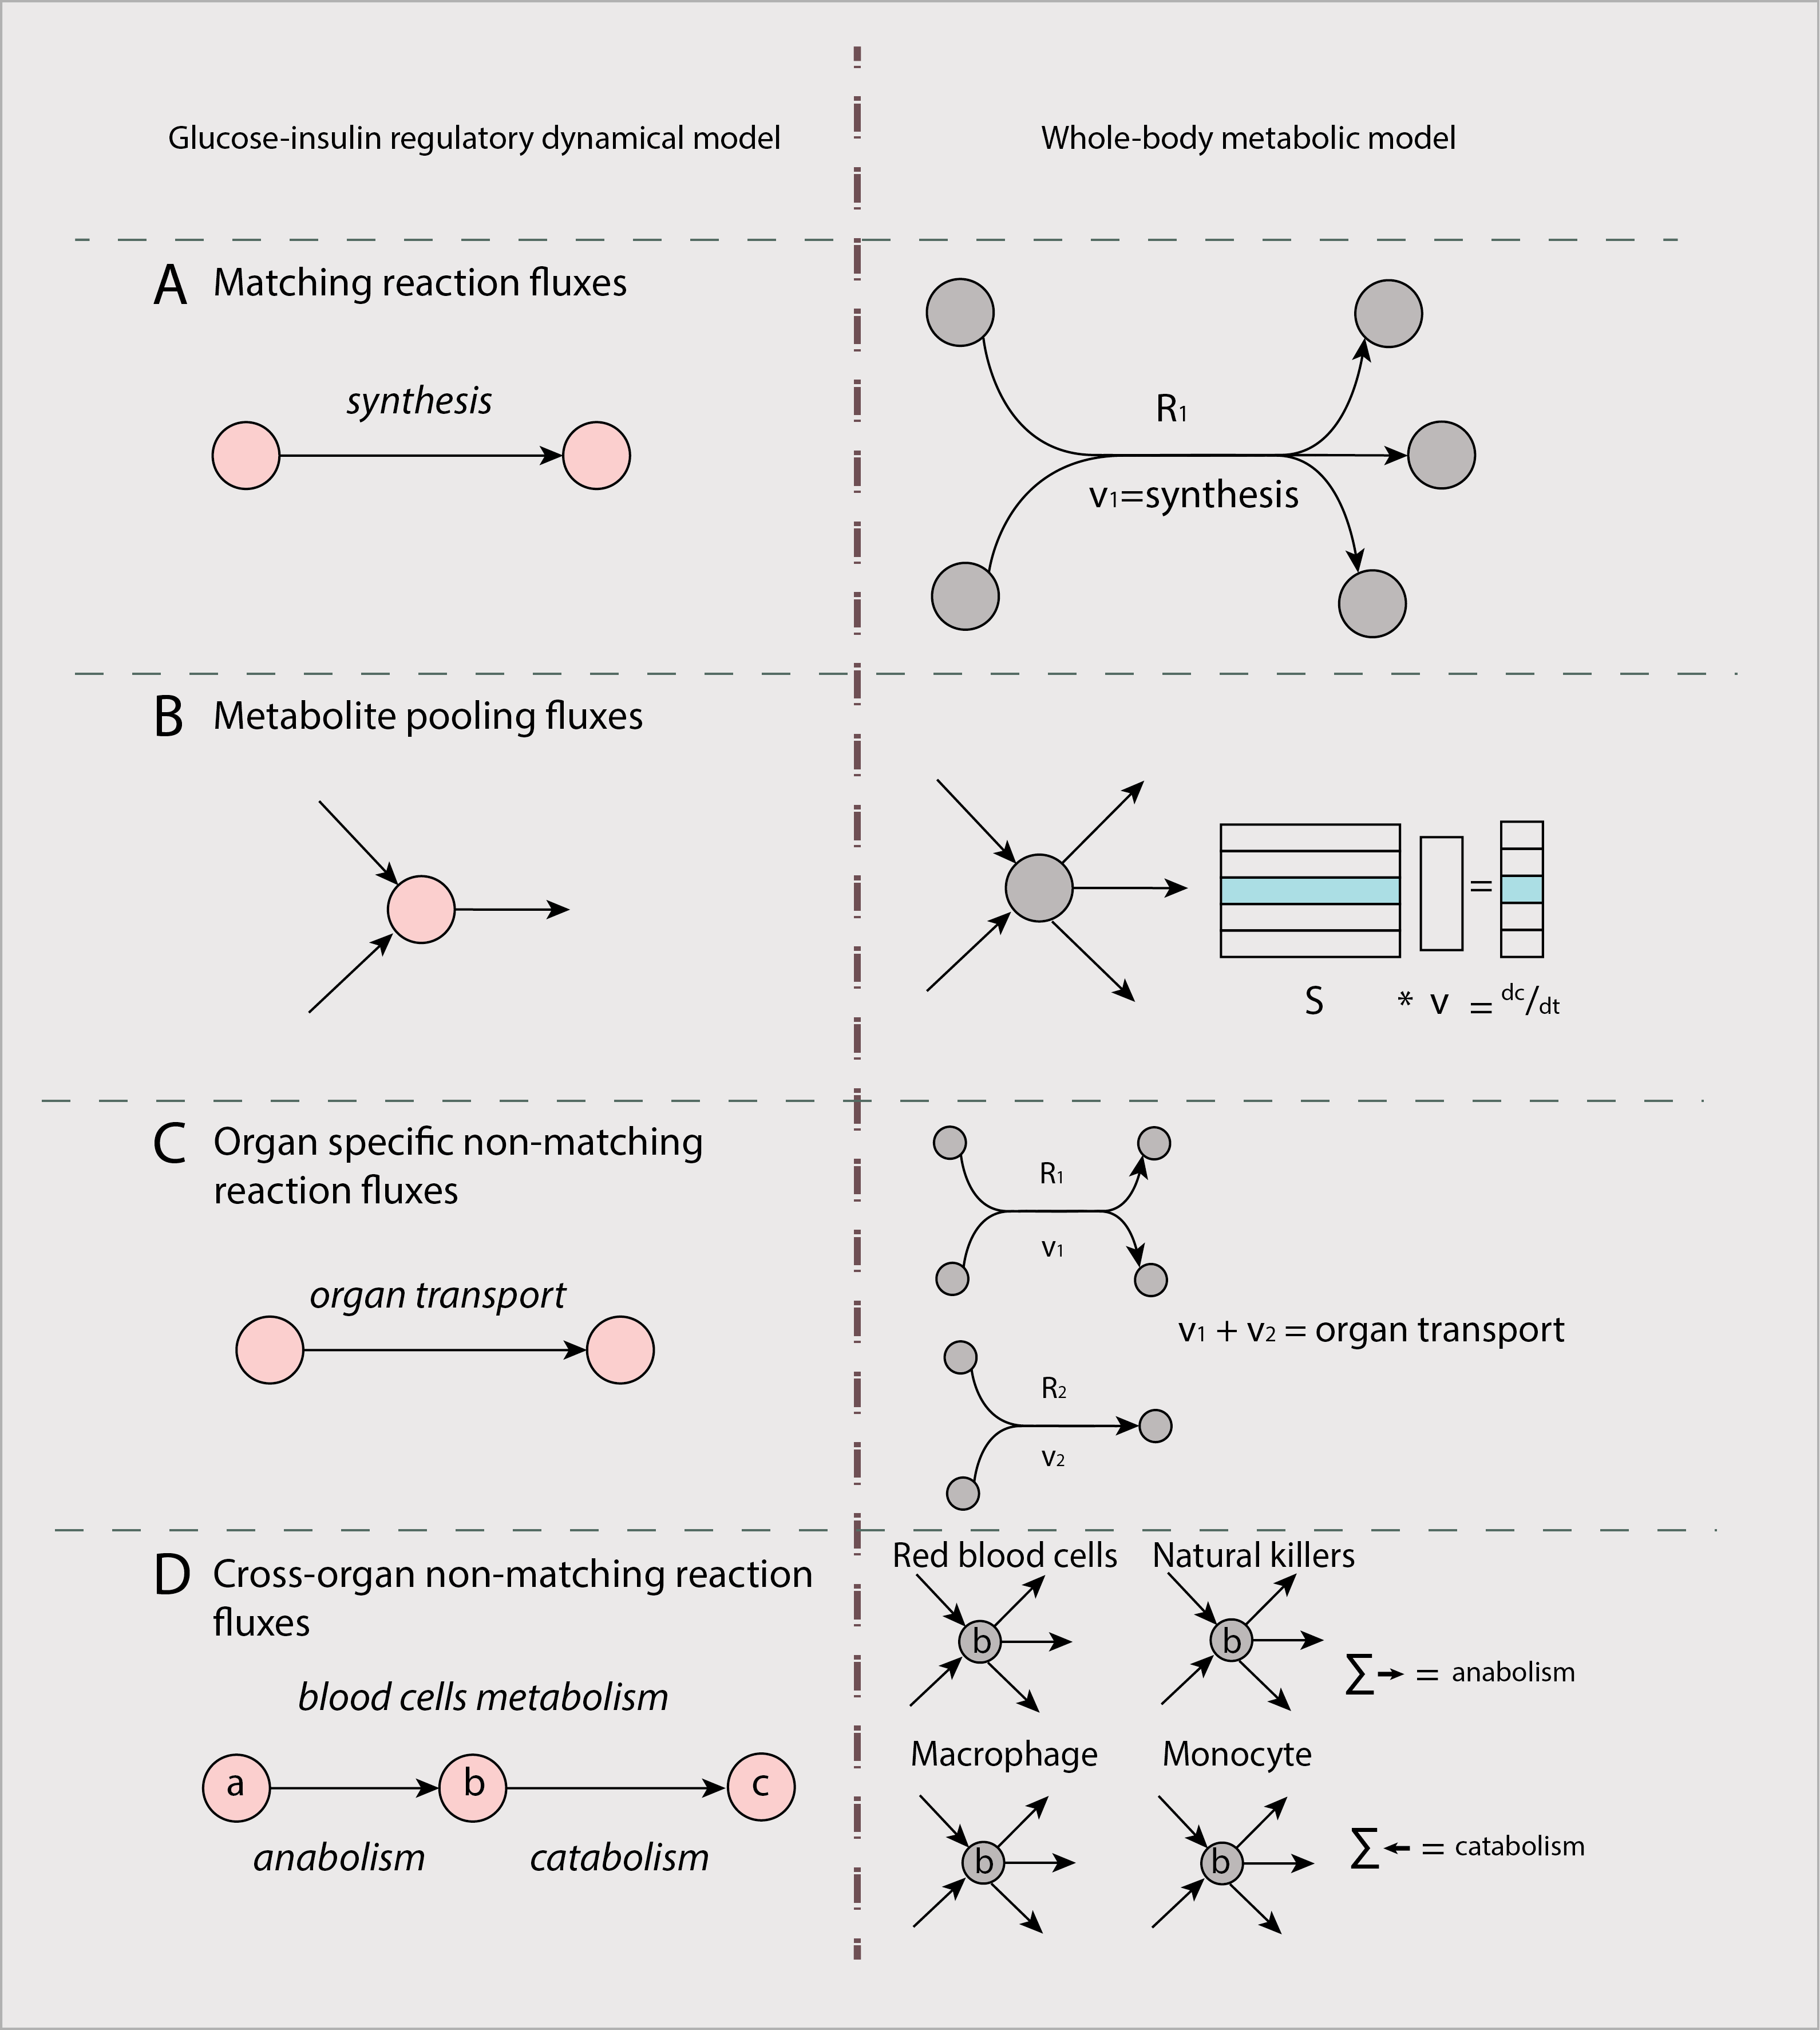
\includegraphics[width=\textwidth,height=\textheight,keepaspectratio]{GIM/figure0.png}%Figure from images\Figure1.png
	\caption[Mapping of dynamical constraints from GIM to Harvey.]{(Continued on the following page)}
	\label{fig:GIM0}
\end{figure}
\begin{figure}[t]
  \contcaption{Subjected constraints from GIM to Harvey. The constraints followed four main scenarii: A- Matching reaction flux corresponds to the case when a reaction in GIM is represented in the same way in Harvey. In this case the fluxes match fully. B-Metabolite pooling fluxes correspond to the case where the rate-of-change of a metabolite in GIM is set as a constraint in the right hand side ($b$ vector) of the linear programming problem in Harvey. C-Organ-specific non-matching reaction fluxes is the case where one reaction in GIM corresponds to more than one reaction in the same organ of Harvey. D-Cross-organ non-matching reaction fluxes. In this case, one tissue in GIM is represented by at least one compartment in Harvey. The sum of cross-organ anabolic (respectively catabolic) fluxes are set equal to the anabolic (respectively catabolic) fluxes in GIM. This case is typically related to blood cells.}% Continued caption
\end{figure}
\section{Results}
Our approach to construct a whole-body model of carbohydrate metabolism consisted of the integration of a dynamical regulatory model of a glucose insulin model (GIM) with a whole-body model of human metabolism (Harvey). The hybrid model (dHarvey) had a better predictive ability than each model on their own and showed notable differences between healthy and type 1 diabetes metabolic states. The off-target effects of both type 1 diabetes and the insulin treatment were modeled at the metabolic level using gene expression data of T1D and the metabolomics of insulin treatment. Therefore, dHarvey included the different scales of glucose metabolism (gene expression, regulation loops and metabolism). The modeling of both the target and off-target effects of T1D and insulin allowed to address the between and within-patient variability to insulin.
\begin{figure}[!htp]
\centering
	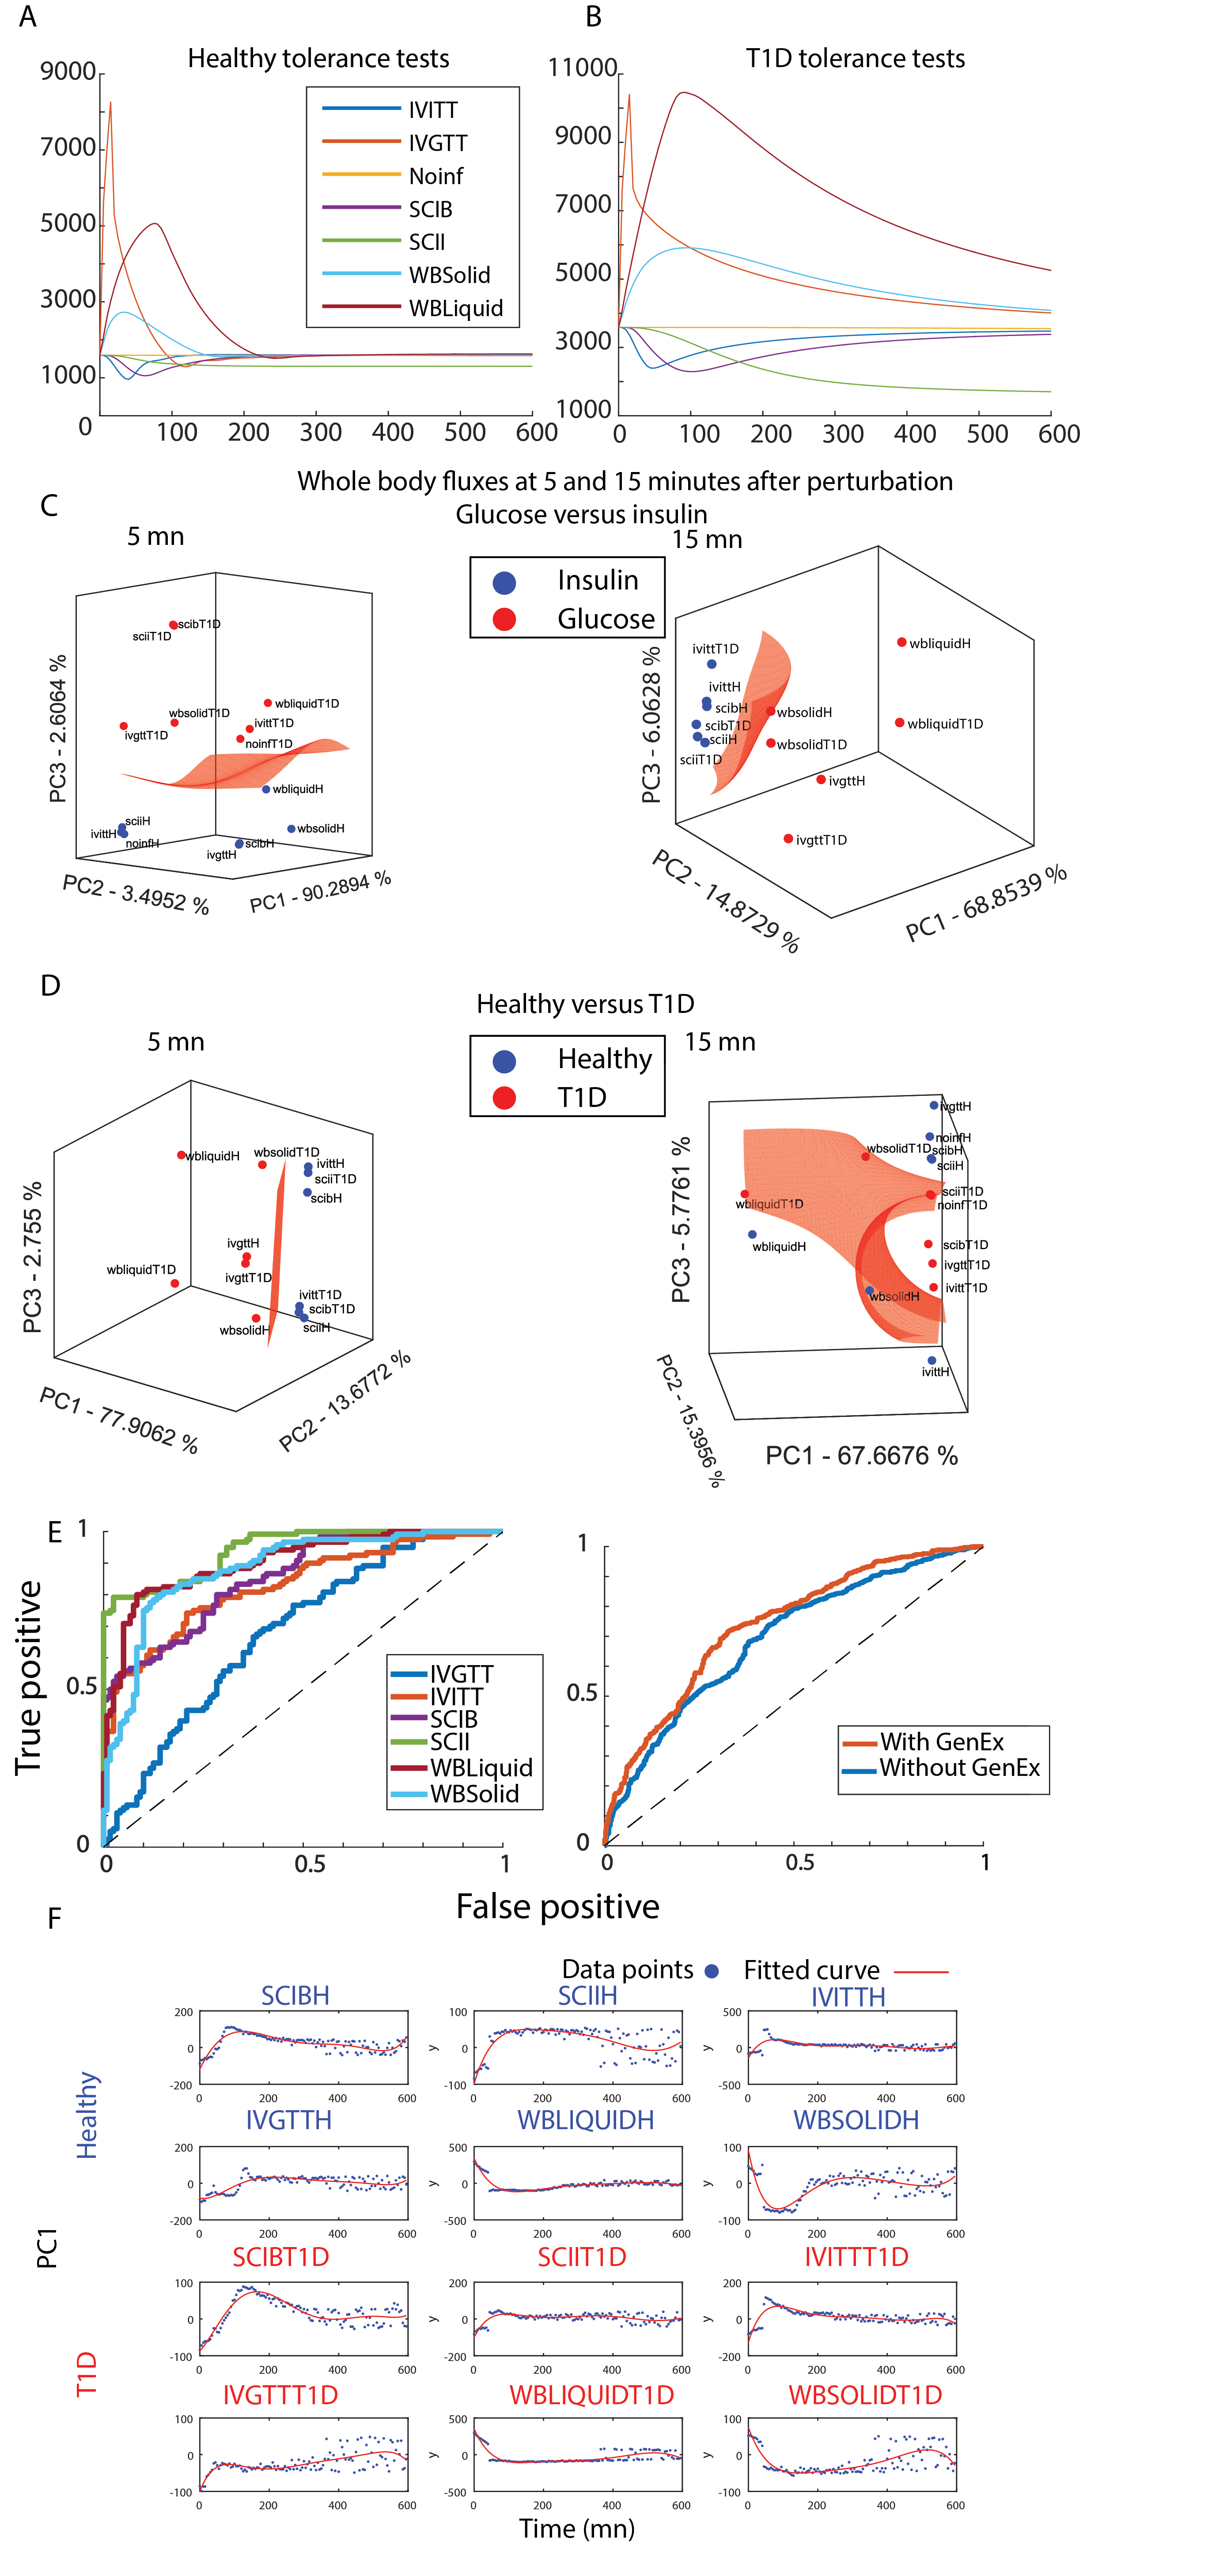
\includegraphics[width=\textwidth,height=\textheight,keepaspectratio]{GIM/figure1.png}%Figure from images\Figure1.png
	\caption[T1D induces a whole-body metabolic shift.]{(Continued on the following page)}
	\label{fig:GIM1}
\end{figure}
\begin{figure}[t]
  \contcaption{Whole-body reaction flux dynamics classify type 1 diabetes and healthy. A-Time course of glucose in peripheral blood in healthy and B-type 1 diabetes in the different tolerance tests using GIM. C-Principal component analysis of whole-body metabolic fluxes in insulin and glucose challenges and D-in healthy and T1D dHarvey models at five and 15 mn after perturbation using three first components. The support vector machine Gaussian boundary was plotted to assess the separation between classes. E-ROC curves of T1D classification. Whole-body flux dynamics over 600 minutes of simulation discriminate between healthy and T1D in each tolerance test alone (left) and in a combination of all tolerance tests in a binary classifier (right), where adding gene expression constraints showed a higher predictive capability of the model towards T1D. F-Time-course of the first principal component (PC1) of the flux vector in each time step in the different tolerance tests showed a shift in global metabolism as a result of glucose dynamics. IVITT: intravenous insulin tolerance test, IVGTT: intravenous glucose tolerance test, Noinf: baseline glucose concentration, SCIB: subcutaneous insulin bolus, SCII: subcutaneous insulin infusion, WBSolid: solid meal, WBLiquid: oral liquid glucose solution.}% Continued caption
\end{figure}
\subsection{Whole body flux dynamics discriminate between healthy and type 1 diabetes and insulin and glucose challenges}
In clinical routine, the diagnosis of diabetes mellitus is confirmed by antibody detection as well as tolerance tests. In order to identify the global metabolic shift induced by T1D and by the glucose or insulin challenges during the tolerance tests, we built dHarvey, a hybrid model including continuous and discrete dynamics. The dynamical simulations of the different tolerance tests in healthy (Figure \ref{fig:GIM1}-A) and type 1 diabetes (Figure \ref{fig:GIM1}-B) using GIM were coupled individually to Harvey (Text \ref{GIM:spsim}) to assess the effects on whole-body, organ-wide metabolic fluxes. Using principal component analysis, we reduced the dimensionality of the predicted fluxes to three dimensions, which captured 95\% of the variability with dHarvey models representing the glucose-insulin-glucagon effects (target effects) only (Figure \ref{fig:GIM1}-C) and 93\% with models additionally including differentially expressed genes (off-target effects) in type 1 diabetes (Figure \ref{fig:GIM1}-D). Using whole-body metabolic fluxes, a Support Vector Machine (SVM) classifier segregated the insulin tests (IVITT, SCIB, SCII) and the glucose tests (IVGTT, WBLiquid, WBSolid) (Figure \ref{fig:GIM1}-C) at five and 15 minutes after perturbation, as well as on all five minute time steps in the 600 minutes of simulation, aggregated in the binary classifier (Figure \ref{fig:s1GIM}, AUROC=0.82). Subjecting additional constraints on the pancreas using type 1 diabetes gene expression data (Table \ref{GIM:tbls1}) allowed to represent metabolic effects that were not directly linked to the decrease of insulin levels and the consequent increase in glucose levels as represented by GIM. The off-target effects were expectedly represented in mainly inflammation and immune system disorders (Figure \ref{fig:s0GIM}-A-B) and the selected 24 metabolic genes (Figure \ref{fig:s2GIM}) still represented the main features of the T1D, e.g., disruption of glucose transport and gluconeogenesis (Figure \ref{fig:s0GIM}-C-D-E).\\ 
The gene expression derived constraints represented both the glycolytic effects and the immune system disruption effect on metabolism which allowed to segregate the whole-body fluxes in healthy and disease models (Figure \ref{fig:GIM1}-D) at five and 15 minutes after perturbation as well as on the whole time horizon of the simulation (Figure \ref{fig:GIM1}-E(left panel), AUROC>0.68). Particularly, classifying glucose and insulin challenges improved (Figure \ref{fig:s1GIM} when gene expression constraints were applied on the pancreas (AUROC=0.82, AUROC=0.8). Furthermore, The classification of T1D improved as well through applying gene expression constraints (Figure \ref{fig:GIM1}-E(right panel), AUROC=0.73) in comparison to the models that were not (AUROC=0.69). This finding highlights the importance of the underlying chronic inflammation in T1D on the patient's metabolism yet the common treatment stays mostly symptomatic and targeted towards glycaemia control. The global metabolic change was further supported by the time course of the first component (PC1) in the different tolerance tests (Figure \ref{fig:GIM1}-F). Finally, the addition of off-target effects of type 1 diabetes using gene expression data on the pancreas enabled to accurately classify T1D and healthy models in the whole-body flux space. The simulations of dHarvey on a whole-body scale was predictive towards both the condition, i.e., T1D, and the challenge, i.e., insulin and glucose, and allows the study of disrupted metabolic pathways in T1D.
\subsection{Differential reaction fluxes between healthy individuals and type 1 diabetes patients}
\begin{figure}[!htp]
\centering
	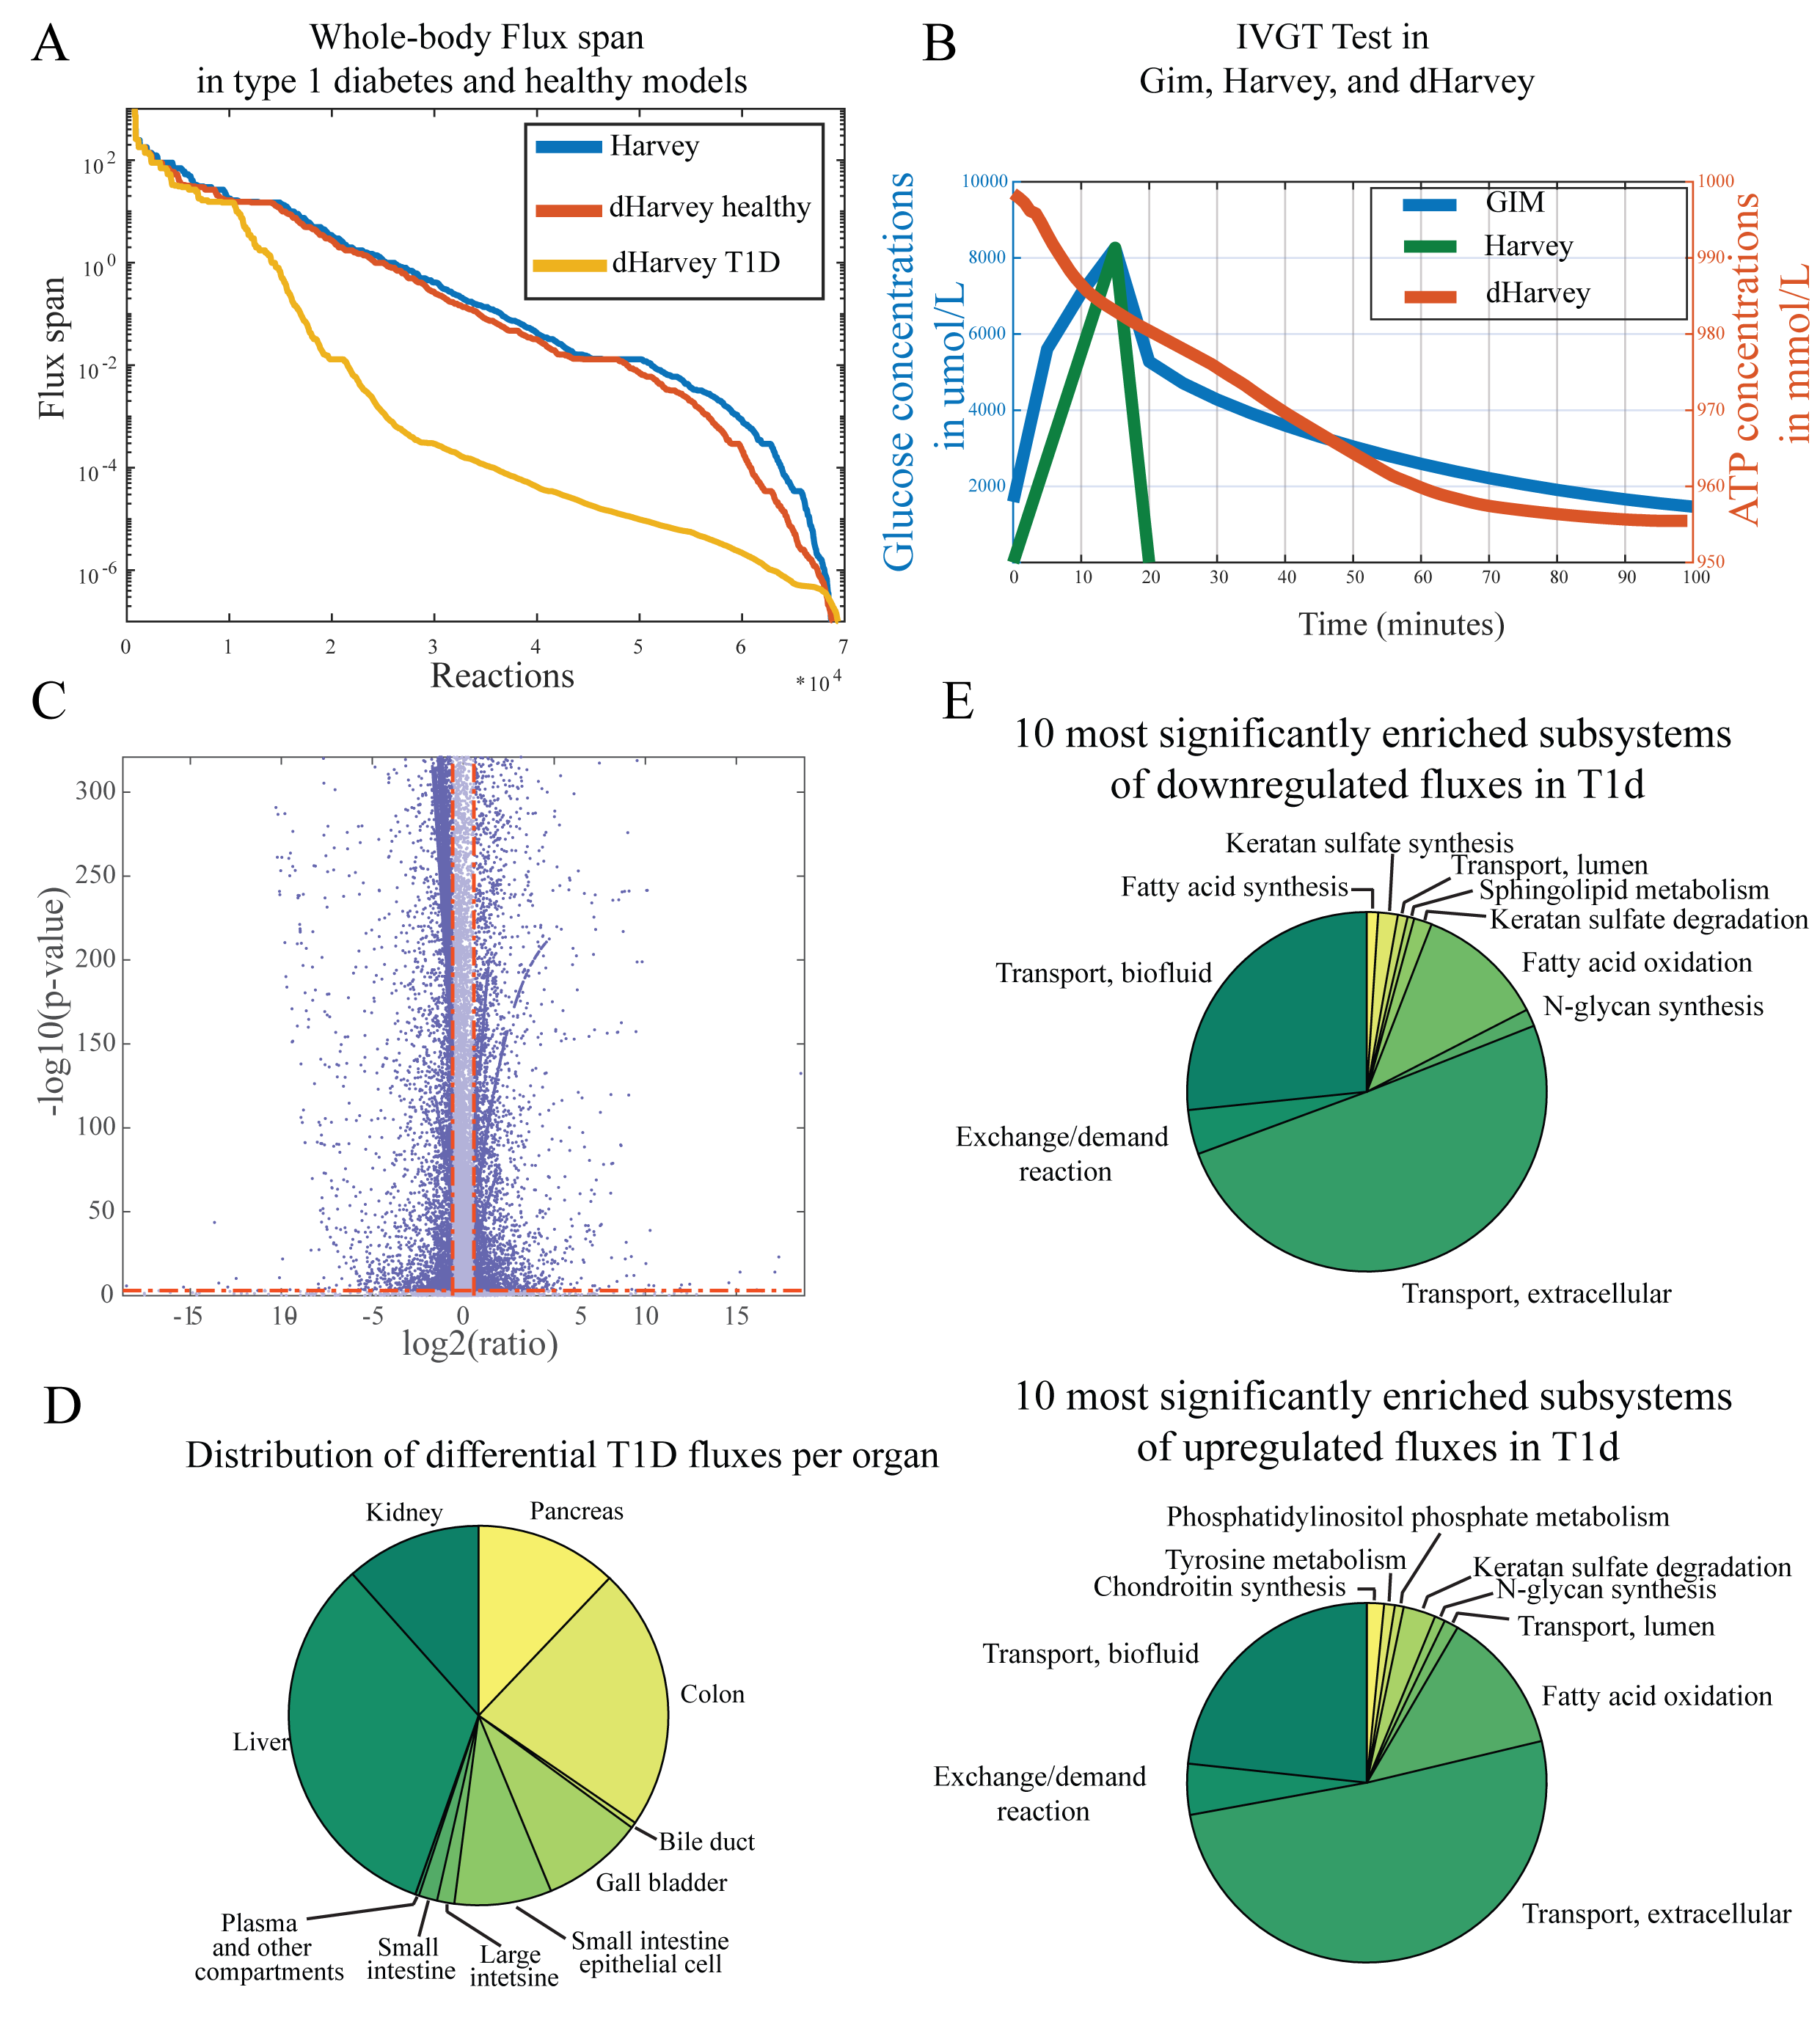
\includegraphics[width=\textwidth,height=\textheight,keepaspectratio]{GIM/figure2.png}%Figure from images\Figure1.png
	\caption[Differential metabolic fluxes between T1D and healthy.]{The multi-scale whole-body model identified disrupted metabolic processes in type 1 diabetes mellitus. A- Flux variability analysis of the pancreas in Harvey in comparison to dHarvey in healthy and type 1 diabetes models. B-Time course of glucose in peripheral blood in intravenous glucose tolerance test modeled by Harvey alone and GIM alone, and ATP theoretical amount in the adipocyte during the IVGTT as predicted by dHarvey. C-volcano plot of differential reaction fluxes (ratio of fold change) in healthy and type 1 diabetes model. D-Differential flux distribution by organ and E- by subsystem (p<0.05).}
	\label{fig:GIM2}
\end{figure}
%\cite{kuleshov2016enrichr, chen2013enrichr} Enrichr citation
In order to capture the non-glycolytic, off-target effects of T1D, we constrained the reaction fluxes in dHarvey by the gene expression of T1D human pancreas and pancreatic islets \cite{planas2010gene}. The differentially expressed set of metabolic genes (Table \ref{GIM:tbls1}) were mapped to Harvey (Figure \ref{fig:s2GIM}) alongside the target effects that were modeled with the constraints arising from GIM. The enriched terms of the selected metabolic genes (Figure \ref{fig:s0GIM}) showed that a large part of the common features of the disrupted processes in diabetes was correctly captured ( in HumanCyc \cite{romero2005computational} and the dbGap \cite{mailman2007ncbi} databases) but also represented shared feature with glucose-involving conditions (Figure \ref{fig:s0GIM}) such as malaria \cite{ogetii2010hypoglycaemia} and type 2 diabetes (in OMIM database) \cite{mailman2007ncbi}.\\
Using flux variability analysis \cite{mahadevan2003effects}, we compared the flux span of pancreatic reactions in unconstrained Harvey and dHarvey model. Harvey had a reduced solution space (Figure \ref{fig:GIM2}-A), as depicted by the flux span, when coupled to GIM. Therefore, the set of obtained solutions is constrained to biologically relevant phenotypes with respect to glucose metabolism. The T1D dHarvey model showed a smaller flux span in comparison to the dHarvey healthy model  (Figure \ref{fig:GIM2}-A), thus a decreased metabolic flexibility and adaptive behaviour towards increased glucose levels and the reduced insulin secretion that shape the disease pathophysiology.
We compared the predictive capabilities of each of Harvey, GIM, and dHarvey with respect to metabolite dynamics in intravenous glucose tolerance test (IVGTT). While GIM natively predicted glucose kinetics with top-down estimated parameters from \textit{in vivo} measured concentrations \cite{schaller2013generic}, Harvey alone fails to predict the glucose dynamics because of lack of insulin and glucagon regulation (Figure \ref{fig:GIM2}-B). dHarvey performs equally well as GIM and is able to predict the dynamics of metabolites involved in imbalanced reactions such as the ATP demand in the adipocyte during IVGTT.\\ 
The baseline glucose levels in healthy and T1D GIM models were as well coupled to Harvey and informed about steady state glucose fluxes. Using dHarvey, we compared the fold change of reaction fluxes in healthy and T1D (Figure \ref{fig:GIM2}-C). FVA was done on the healthy and T1D irreversible models (where all reactions are irreversible) to guarantee positive flux values for the consequent fold change analysis. The FVA solutions were subsequently stored, resulting in 160,032 (number of reaction times two) flux values per reaction. Using the obtained data, we were able to compare flux distributions as opposed to single flux values (Text \ref{GIM:sp5}). A fold change analysis was then performed on the flux distributions.
The obtained volcano plot showed the significantly different reaction fluxes in both conditions. A total of 33,526 reactions over a total of 80,016 reactions exhibited a change in value between the conditions, of which 6,602 were increased and 15,205 were decreased significantly above 50\% (fold change greater than 1.5) of their healthy values (p<0.001). Reaction enrichment in metabolic subsystems (Figure \ref{fig:GIM2}-D) and organs (Figure \ref{fig:GIM2}-E) showed an expected systematic and ubiquitous deregulation of glucose metabolism, particularly in target organs (pancreas, liver, and kidney). 
The subsystem for transport reactions is the most affected since it covers glucose exchange from producing organs, e.g., glycogenolysis in the liver to energy-requiring processes. Overall, the differential fluxes of reactions were related to known semiology of T1D in the different organs (Table \ref{GIM:tbls4}), e.g., cardiovascular disease, retinopathy, ketoacidosis, and liver glycogen deposition. 
Of notable difference, the disruption of the transport system in T1D (Figure \ref{fig:GIM2}-E) suggested a prominent role of insulin in maintaining a global inter-organ communication. We will investigate this aspect in the next section.

\subsection{Prediction of exogenous insulin off-target effects}

\begin{figure}[!htp]
\centering
	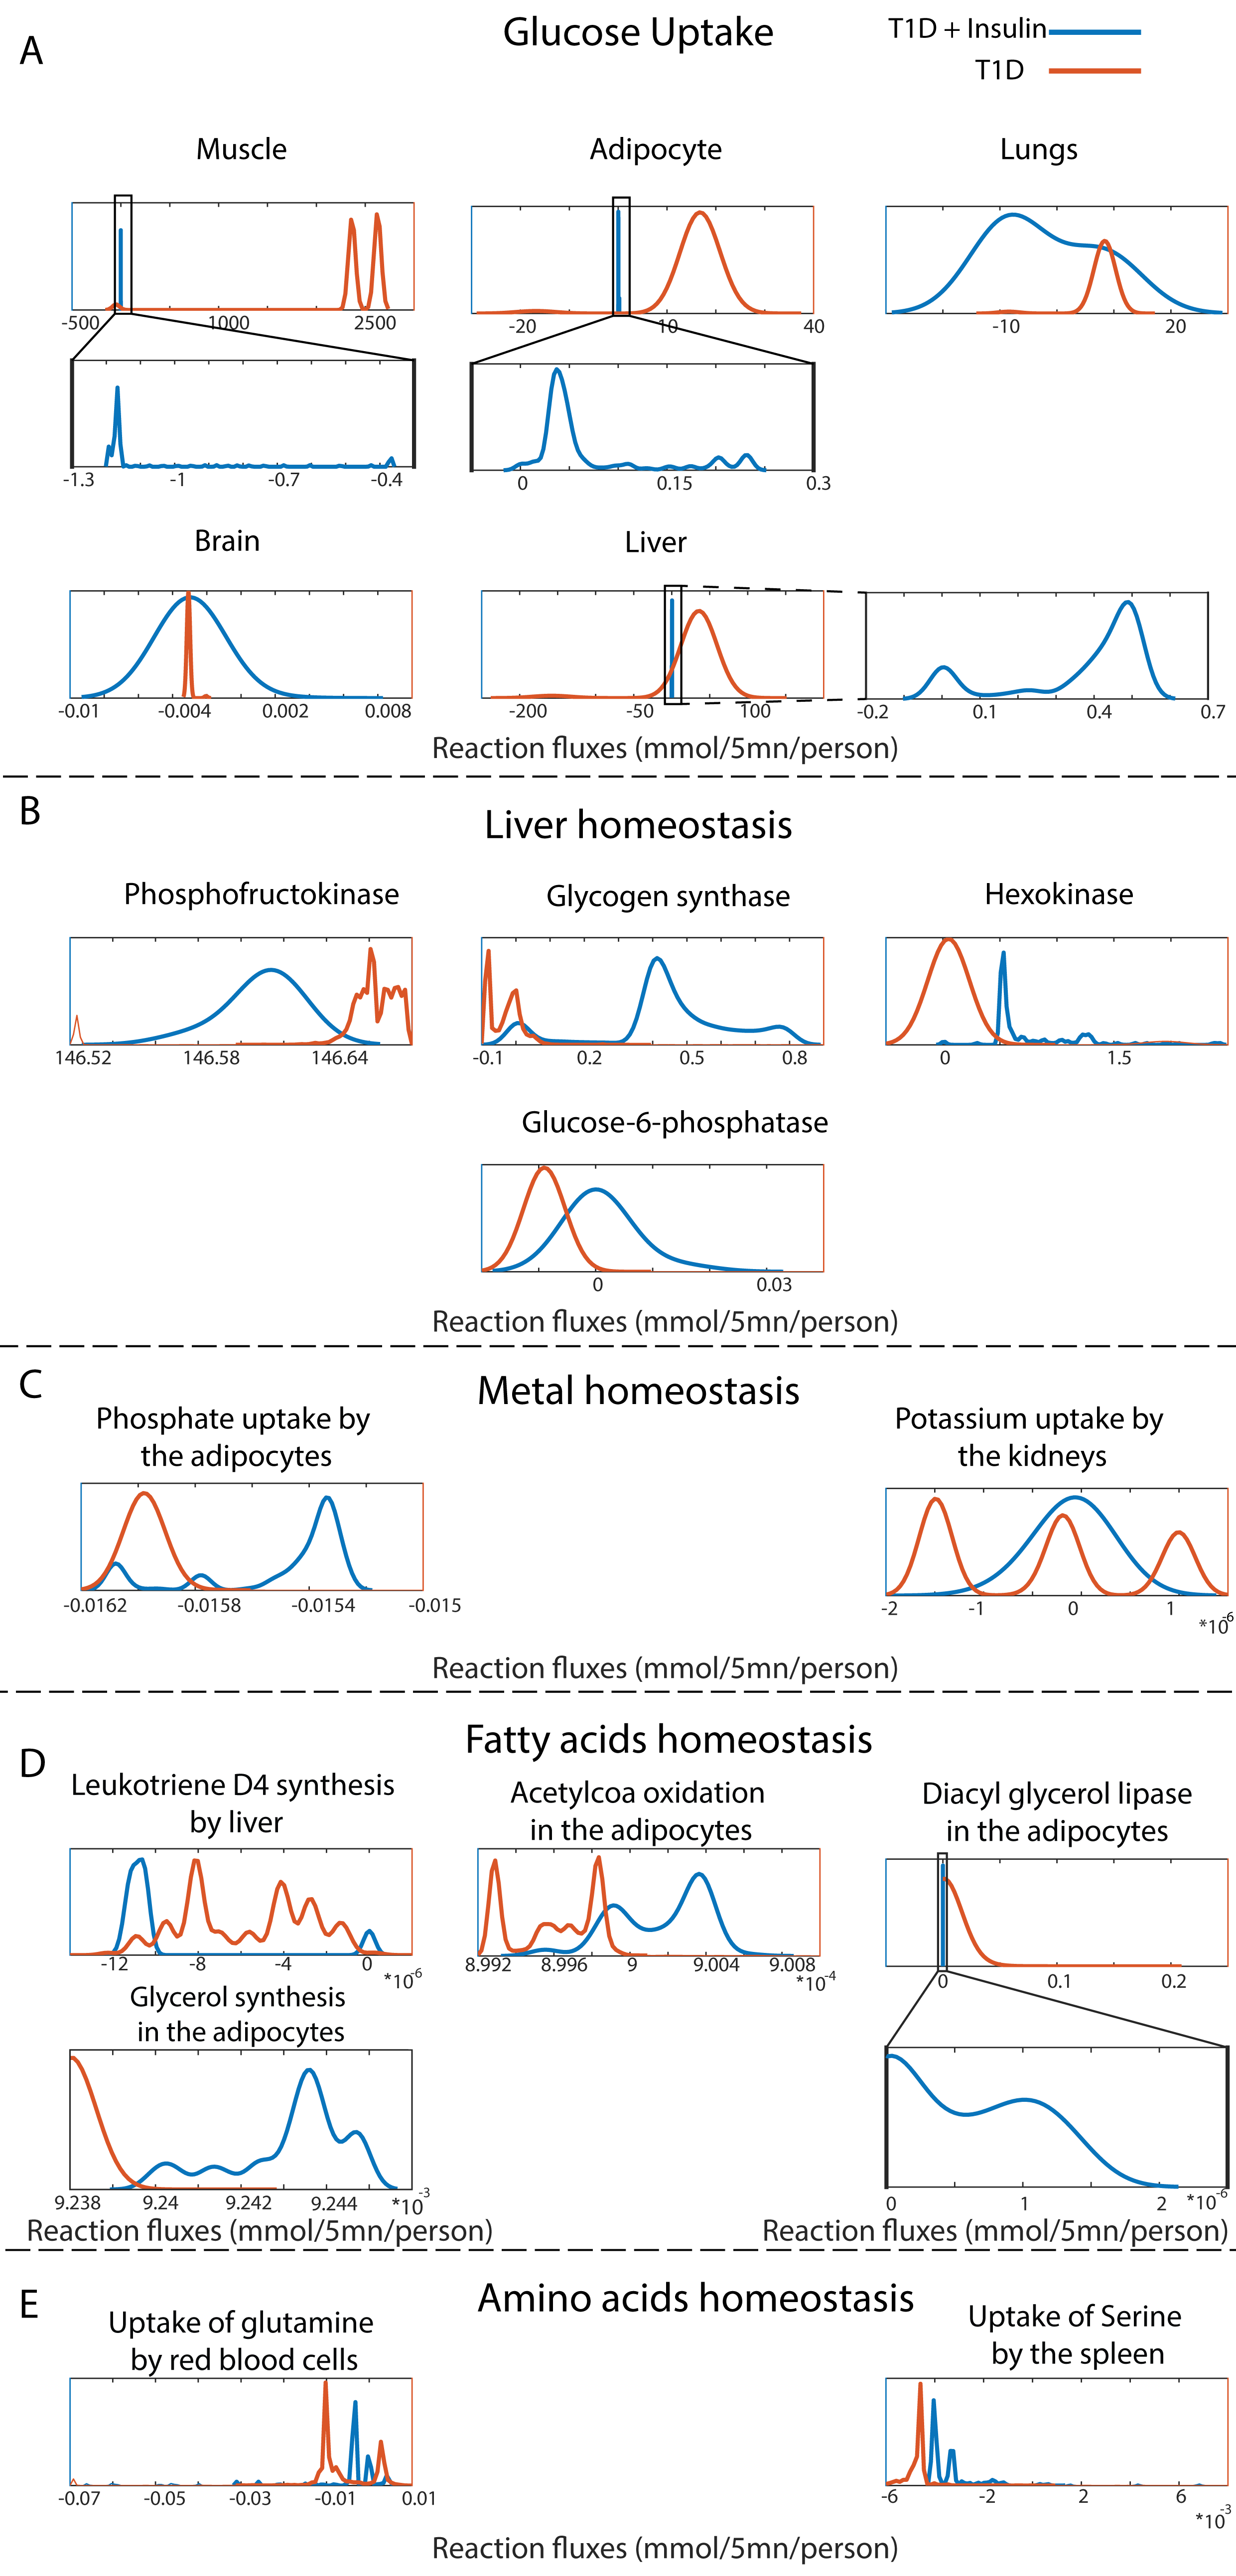
\includegraphics[width=\textwidth,height=\textheight,keepaspectratio]{GIM/figure3.png}%Figure from images\Figure1.png
	\caption[Insulin metabolic off-target effects.]{(Continued on the following page)}
	\label{fig:GIM3}
\end{figure}
\begin{figure}[t]
  \contcaption{Insulin metabolic off-target effects assessed by the probability density estimates of reaction flux values. The fluxes include A-glucose uptake, B-liver glycolytic reactions, C-metal homeostasis, D-fatty acids reactions and E-amino acids uptake, in various organs after a subcutaneous insulin administration.}% Continued caption
\end{figure}

The physiological effects of insulin mainly affect the uptake of glucose by organs. A recent study \cite{yugi2014reconstruction} suggested  a regulation of the liver isoform of phosphofructokinase (PFK) by insulin such that upstream fluxes of PFK are downregulated and downstream fluxes upregulated. Dynamics of liver glycolysis fluxes in subcutaneous insulin bolus setting (Figure \ref{fig:GIM3a}) confirmed three out of eight regulatory flux patterns, while one flux remained invariant and four were mispredicted. As this new insight was not captured in dHarvey, we used an additional dynamical model \cite{yugi2014reconstruction} to represent the off-target effects of insulin in the liver. The ODE model was coupled to dHarvey which now captures both T1D and insulin target and off-target effects. In addition to glycolysis, insulin influences amino acids uptake, particularly large and neutral ones (LNAA), resulting in a decrease in blood concentrations of LNAA. The model predicted a decrease in all LNAAs in the blood (Figure \ref{fig:GIM3a}) after 60 minutes of insulin administration, preceded by a transient increase at 30 minutes.
In order to infer the metabolic effects of insulin, interpreting single solutions of dHarvey proves ineffective given the high dimensionality of the model and the alternate optimal solution (AOS) space. To characterize the AOS space, FVA provided an empirical flux probability density per reaction. We compared the probability density estimates of the fluxe values in T1D with and without insulin administration. Glucose uptake expectedly increased in the muscle, adipocytes, and lungs while remaining unchanged in the liver and brain (Figure \ref{fig:GIM3}), as expected given their vital role. Insulin stimulated the activity of phosphofructokinase, glycogen phosphatase, and hexokinase while inhibiting glucose-6-phostphatase, contributing to its overall anabolic effect. The uptake of phosphate by the adipocytes also increased, which links to the known depletion  of metals after continuous insulin injection, while the uptake of potassium did not change significantly. In relation to the fatty acids biosynthesis, insulin enhanced the synthesis of lipoproteins in the liver, inhibited the oxidation of fatty acids and the diacyl glycerol lipase in the adipocytes. The prediction of triglycerides levels using CRONICS (Figure \ref{fig:GIM3b}), showed an increase in the adipocytes following the administration of insulin. Finally, the uptake of glutamine in the red blood cells and serine in the spleen, taken as example (Figure \ref{fig:GIM3}), supported our findings regarding the higher insulin-induced uptake of amino acids.\\
Moreover, we investigated the anabolic effect of insulin on inter-organ crosstalk. Due to large running times, the simulation of the dHarvey model using CRONICS framework restricted the distance minimization of the flux vectors between the different time steps (Figure \ref{fig:s3GIM}-step VI) to a subvector including pancreas, kidney, adipocytes, muscle, liver, brain, and fluids, e.g., peripheral blood, portal vein, blood brain barrier, intestinal compartments. The comparison of the inter-organ crosstalk in dHarvey after insulin administration to the T1D steady state showed an increase in the metabolites exchange set, particularly in the muscle, kidney, brain, and liver (Figure \ref{fig:GIM3c}). The total number of exchanged metabolites in T1D model equalled 229 exchanged metabolites while insulin induced an exchange of 297 metabolites overall. 
Finally, having constructed dHarvey, a dynamical hybrid model of type 1 diabetes and insulin response, we investigated the effects of within and between patient response to insulin administration.
\subsection{Between-subject variability is reflected in citric acid cycle and oxidative phosphorylation}
Using the dHarvey model representing both T1D and insulin target and off-target effects, we investigated the mechanisms underlying inter-individual variability. A set of kinetic parameters of the GIM model with differential values in T1D and healthy individuals (Table \ref{GIM:tbl1}) \cite{schaller2013generic} was varied (Figure \ref{fig:GIM4}-A) to reproduce the clinically observed 25-35\% \cite{heinemann2002variability} of inter-individual variability in 31 synthetic type 1 diabetes patients (30 simulated patients and 1 reference average patient) (Figure \ref{fig:GIM4}-B). The obtained between-subject variability equalled 30.11\%, in agreement with the empirical values. For every synthetic patient, the personalized dHarvey was simulated for 600 minutes after the subcutaneous injection of insulin bolus.\\
\begin{table}[!htp]
\caption[Selected whole-body parameters in inter-individual variability simulations.]{Selected whole-body parameters in inter-individual variability simulations.}
\begin{center}
	\begin{tabular*}{\textwidth}{l @{\extracolsep{\fill}} ll}
	\hline
	Parameter & GIM path  & Description         \\ 
	\hline
	P\_1711    & Liver|Interstitial|Glucagon\_0 & Baseline glucagon level in the liver   \\
	P\_2049    & Pancreas|Interstitial|Insulin\_0 & Baseline insulin level in the pancreas \\
	P\_322          & Fat|Endosome|End\_IR\_0 & Adipocyte baseline insulin receptor \\
	& & in the endosome \\
	P\_1757/P\_1755  & Liver|Intracellular|End\_IR\_0\_liv & Liver baseline insulin receptor in the cell \\
	P\_1978 & Muscle|Endosome|End\_IR\_0  & Muscle baseline insulin receptor in\\
	& & the endosome      \\
	P\_323          & Fat|Endosome|End\_IRp\_0  & Adipocyte baseline insulin phosphorylated\\
	& & receptor in the endosome        \\
	P\_1760         & Liver|Intracellular|End\_IRp\_0\_liv & Liver baseline insulin phosphorylated\\
	& & receptor in the cell \\
    P\_1979 & Muscle|Endosome|End\_IRp\_0        & Muscle baseline insulin phosphorylated\\
    & & receptor in the endosome     \\
    P\_293            & Fat|Intracellular|IR\_cell\_0 & Total concentration of adipocyte\\
    & & intracellular insulin receptor \\
    P\_1753          & Liver|Intracellular|IR\_cell\_0 & Total concentration of liver intracellular\\
    & & insulin receptor   \\
	P\_1950    & Muscle|Intracellular|IR\_cell\_0 & Total concentration of muscle intracellular\\
	& & insulin receptor \\
	P\_294          & Fat|Intracellular|IR\_p\_0 & Adipocyte baseline insulin phosphorylated\\
	& & receptor in the cell   \\
	P\_1758/P\_1727            & Liver|Intracellular|IR\_p\_0 & Liver baseline insulin phosphorylated  \\
	& & receptor in the cell \\
	P\_1949 & Muscle|Intracellular|IR\_p\_0 & Muscle baseline insulin phosphorylated       \\
	& & receptor in the cell \\
	P\_1814          & Liver|ReceptorRecyclingFactor-End  & Liver receptor recycling factor\\
	& & in the endosome        \\
	P\_1994         & Muscle|ReceptorRecyclingFactor & Muscle receptor recycling factor \\
    P\_338 & Fat|ReceptorRecyclingFactor        & Adipocyte receptor recycling factor     \\
    P\_1811            & Liver|ReceptorRecyclingFactor & Liver receptor recycling factor \\
	\hline
	\end{tabular*}
\end{center}
\label{GIM:tbl1}%descriptive label to refer to figure in text
\end{table}
The distribution of active reactions across patients and across time was very similar (Figure \ref{fig:GIM4}-C, Figure \ref{fig:s4GIM}), which indicated a similar metabolic network topology. Reducing the dimensionality of flux distribution through PCA (Figure \ref{fig:GIM4}-D) showed that the observed change is driven by the modulation of reaction flux values across time following the action of insulin. Particularly, the end metabolic state was different than the initial state, confirming a metabolic change as an action of insulin. Moreover, each individual had a differential metabolic shift reflective of a quantitative variation in flux values across pathways (Figure \ref{fig:GIM4}-E). Interestingly, we observed that insulin exerted a hysteresis between peripheral glucose concentrations and whole-body metabolism (Figure \ref{fig:GIM4}-F), that was achieved differently between the different individuals.\\
Additionally, we investigated the impact of inter-individual variability on the different metabolic pathways. Particularly, pentose phosphate pathway and glycolysis were remarkably robust towards insulin-induced perturbation, while citric acid cycle and oxidative phosphorylation total whole-body flux over time showed a patient-specific variation (Figure \ref{fig:GIM4}-G). Furthermore, we investigated the effect of intra-individual variability to insulin response on whole-body metabolism.
\subsection{Within-subject variability to insulin}
\begin{figure}[!htp]
\centering
	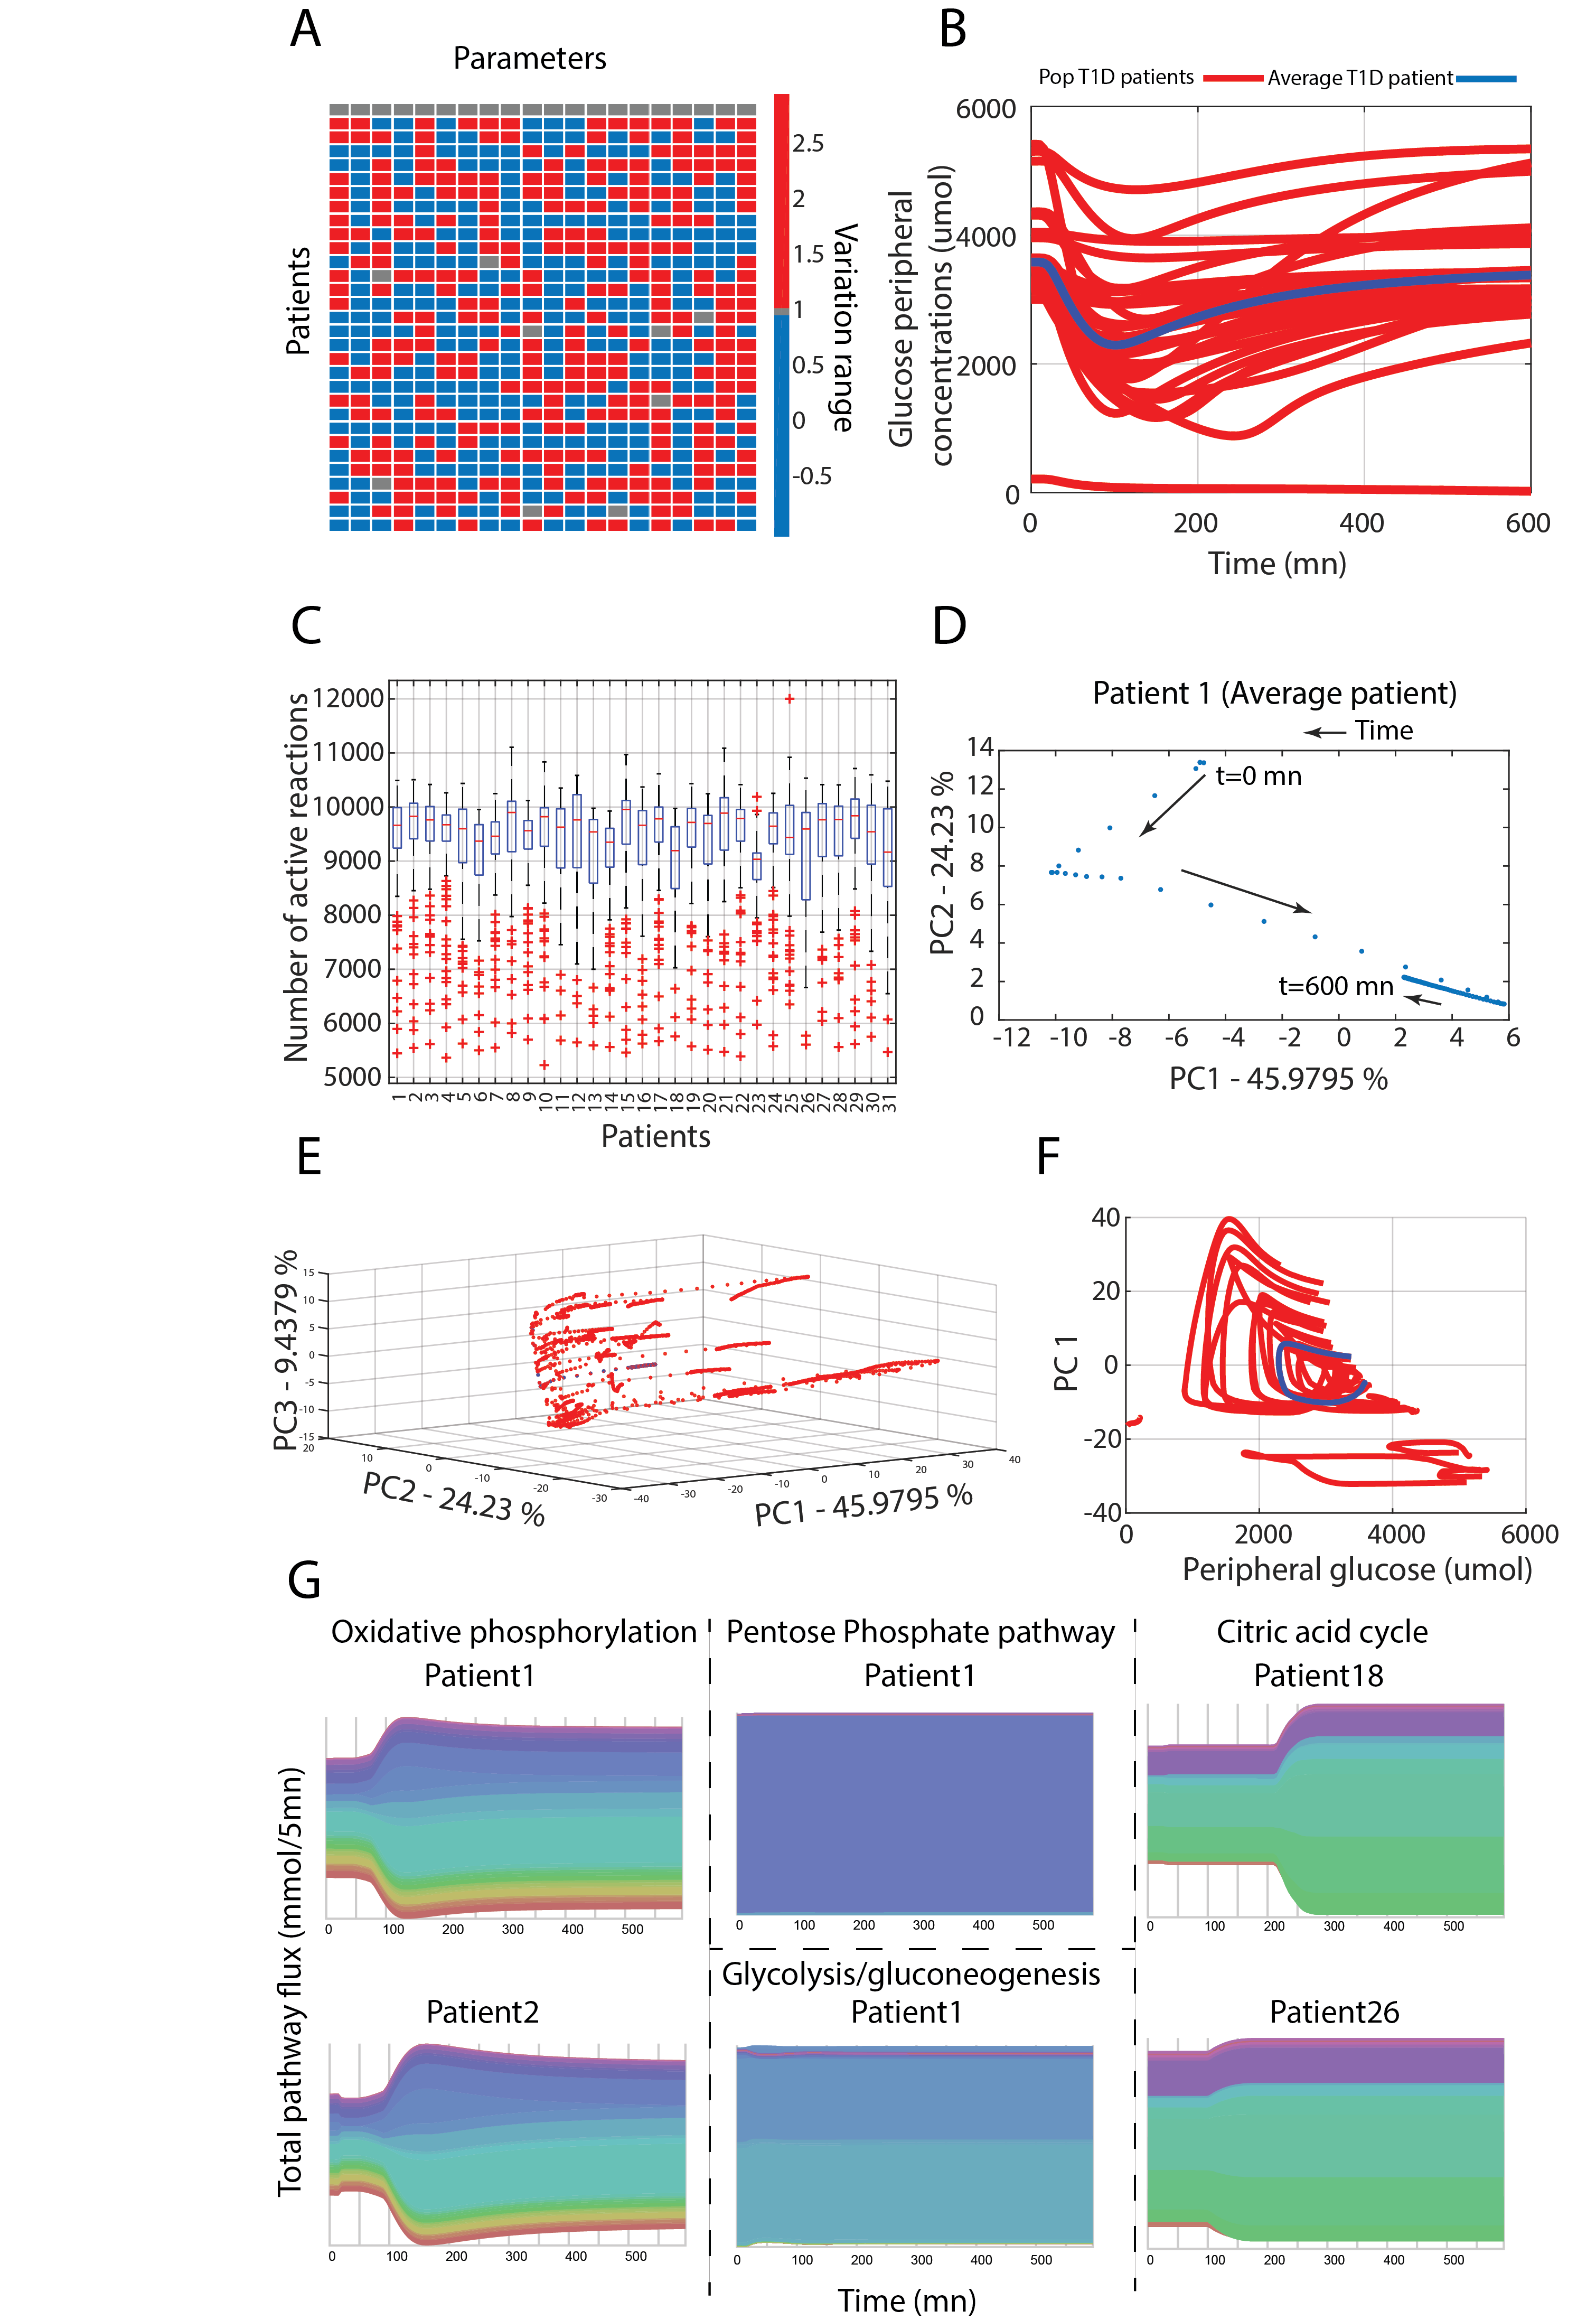
\includegraphics[width=\textwidth,height=\textheight,keepaspectratio]{GIM/figure4.png}%Figure from images\Figure1.png
	\caption[Inter-individual variability to insulin response.]{(Continued on the following page)}
	\label{fig:GIM4}
\end{figure}
\begin{figure}[t]
  \contcaption{Inter-individual variability to insulin response is reflected on key pathways of metabolism. A- Varying a set of individual parameters within the reported inter-individual variability range in the dynamical model yields B- different peripheral glucose concentrations as a response to insulin injection. C- Distribution of the active reactions over simulation time per patient. D- Evolution of the metabolic fluxes as represented by PCA over simulation time of the average patient (patient 1) and E- the population of synthetic patients. F- Insulin-induced hysteresis between glucose peripheral blood levels and whole-body metabolism. G- Citric acid cycle and oxidative phosphorylation total flux reflect between-patient variability while glycolysis and pentose phosphate pathways are stable to perturbation. The flow chart was done using Rawgraphs \cite{Mauri:2017:RVP:3125571.3125585}.}% Continued caption
\end{figure}
Within-subject variability to insulin results from internal, endogenous factors that are specific to a particular metabolic state of the individual, e.g., postprandial state, physical activity. In order to determine the influence of the metabolic state on peripheral glucose dynamics, we set the kinetic parameters of the simulated patient to the reported population mean in GIM and varied the metabolic reactions. In each metabolic state, we generated random objective coefficient weights to every reaction (Figure \ref{fig:GIM5}-A). The weights could be lower, higher, or equal to the mean profile. In the latter case, the simulated profile approached the predictions of the GIM model. To each set of internal perturbations (input) to metabolism, i.e., increase or decrease in reactions weights, we measured the minimal glucose concentration and the final concentration after 10 hours of subcutaneous insulin injection (output) \cite{sarkar2010regression}. In all cases, the time step was decreased from five minutes to 2.5 minutes as both integration failures and conflicting constraints arose from higher time steps.  In the described setting, the reactions of dHarvey fell under two classes, the reactions proper to Harvey and those shared by both GIM and Harvey, referred to as interface reactions \cite{wadehn2016multiscale}. Changing the coefficients of the interface reactions only and simulating dHarvey with FBA for 10 metabolic states resulted in a smooth set of glucose dynamics (Figure \ref{fig:GIM5}-B). In order to get a complete view of the within-patient variability, the reactions proper to the Harvey were included as well. Using FBA to simulate 10 metabolic states of the hybrid model, the glucose profiles showed non smooth profiles, with non-biological concentrations or terminated in the course of simulation (Figure \ref{fig:GIM5}-C).  Finally, performing the simulation using CRONICS ensured both smoothness of the system and minimal debugging to resolve conflicting constraints (Figure \ref{fig:GIM5}-D), of which only 2 simulations permanently failed as they have reached a null concentration of glucose and were removed from subsequent analysis. The 29 metabolic states simulated with the final setting resulted from the perturbation of a total of 2817 reaction. Each metabolic state consisted of a set of perturbed reaction activity as depicted by the random coefficient matrix (Figure \ref{fig:GIM5}-E).
The computed intra-individual variability equalled 30\% \textit{in silico} and was in agreement with the empirical value of 12-45\% \cite{heinemann2002variability}. To determine the influence of every reaction to the metabolic profile of glucose, a multivariate regression was performed using the coefficients matrix as input and a matrix of glucose concentrations per state as output. The minimal and final glucose concentrations were considered for the sensitivity analysis as they inform about adverse reactions and treatment efficacy, i.e., hypoglycemia and hyperglycemia. The reaction sensitivities to both of the readouts (Figure \ref{fig:GIM5}-F) showed that GLUT4 transport had a great share of the influence on glucose profile. Interestingly, reactions from the bile acid synthesis pathway modulated the peripheral glucose profile as well.  Taken together, these findings showed that internal reactions in Harvey, that were not in necessarily in the interface reactions set, had the potential to modulate the glucose concentrations in GIM, through glycolytic and non-glycolytic pathways, thereby suggesting novel approaches to achieve diabetes control.
\section{Discussion}
We developed a multi-scale, dynamic, and organ-resolved model through multi-algorithm integration of metabolic and regulatory processes in T1D. The short time scale insulin-glucose-glucagon regulatory dynamics (GIM) served as constraints to the whole body metabolic network (Harvey). In addition to the expected target effects, the mechanism-unrelated metabolic effects of both insulin and type 1 diabetes pathophysiology were included in the model through organ-specific gene expression data and metabolomics time-course. The integrative model provided a complete picture on the network dynamics, regulation, and response to perturbation and links it to known symptoms and clinically relevant variability of insulin response both within and between-subject.  
\subsection{Chronic inflammation in type 1 diabetes improves disease identification using whole-body fluxes}
In order to assess the impact of the tolerance tests on the whole-body level, the metabolic model (Harvey) was constrained by the glucose-insulin-glucagon regulation modelled by GIM in insulin and glucose challenges involving healthy and T1D states. The metabolic fluxes were consequently used as features in an SVM binary classifier \cite{shaked2016metabolic}. Identifying insulin versus glucose challenges at five minutes and 15 minutes after perturbation was possible due to the opposite effects that these substances induced on the human body (Figure \ref{fig:GIM1}-C). The identification of healthy and T1D flux distribution improved the separation between healthy and T1D individuals after the addition of gene expression constraints in T1D, representing the chronic inflammation that triggers the pathogenesis of the disease. While glycaemia control is achieved through allopathy, the inflammatory aspect of the disease is often overlooked \cite{mccall2013treating} and has to be equally addressed. In addition, it was possible to define a healthy and diabetic boundary using whole-body metabolic fluxes despite the subjected constraints affected mainly the glucose-related pathways (Figure \ref{fig:GIM1}-D). These findings further reinforce the idea that type 1 diabetes is a multifactorial, pan-organ and systemic disease because of the key role that glucose plays in regulation of metabolism and energy.
\subsection{Differentially regulated fluxes suggest mechanisms underlying the systemic symptomatology of type 1 diabetes}
\begin{figure}[!htp]
\centering
	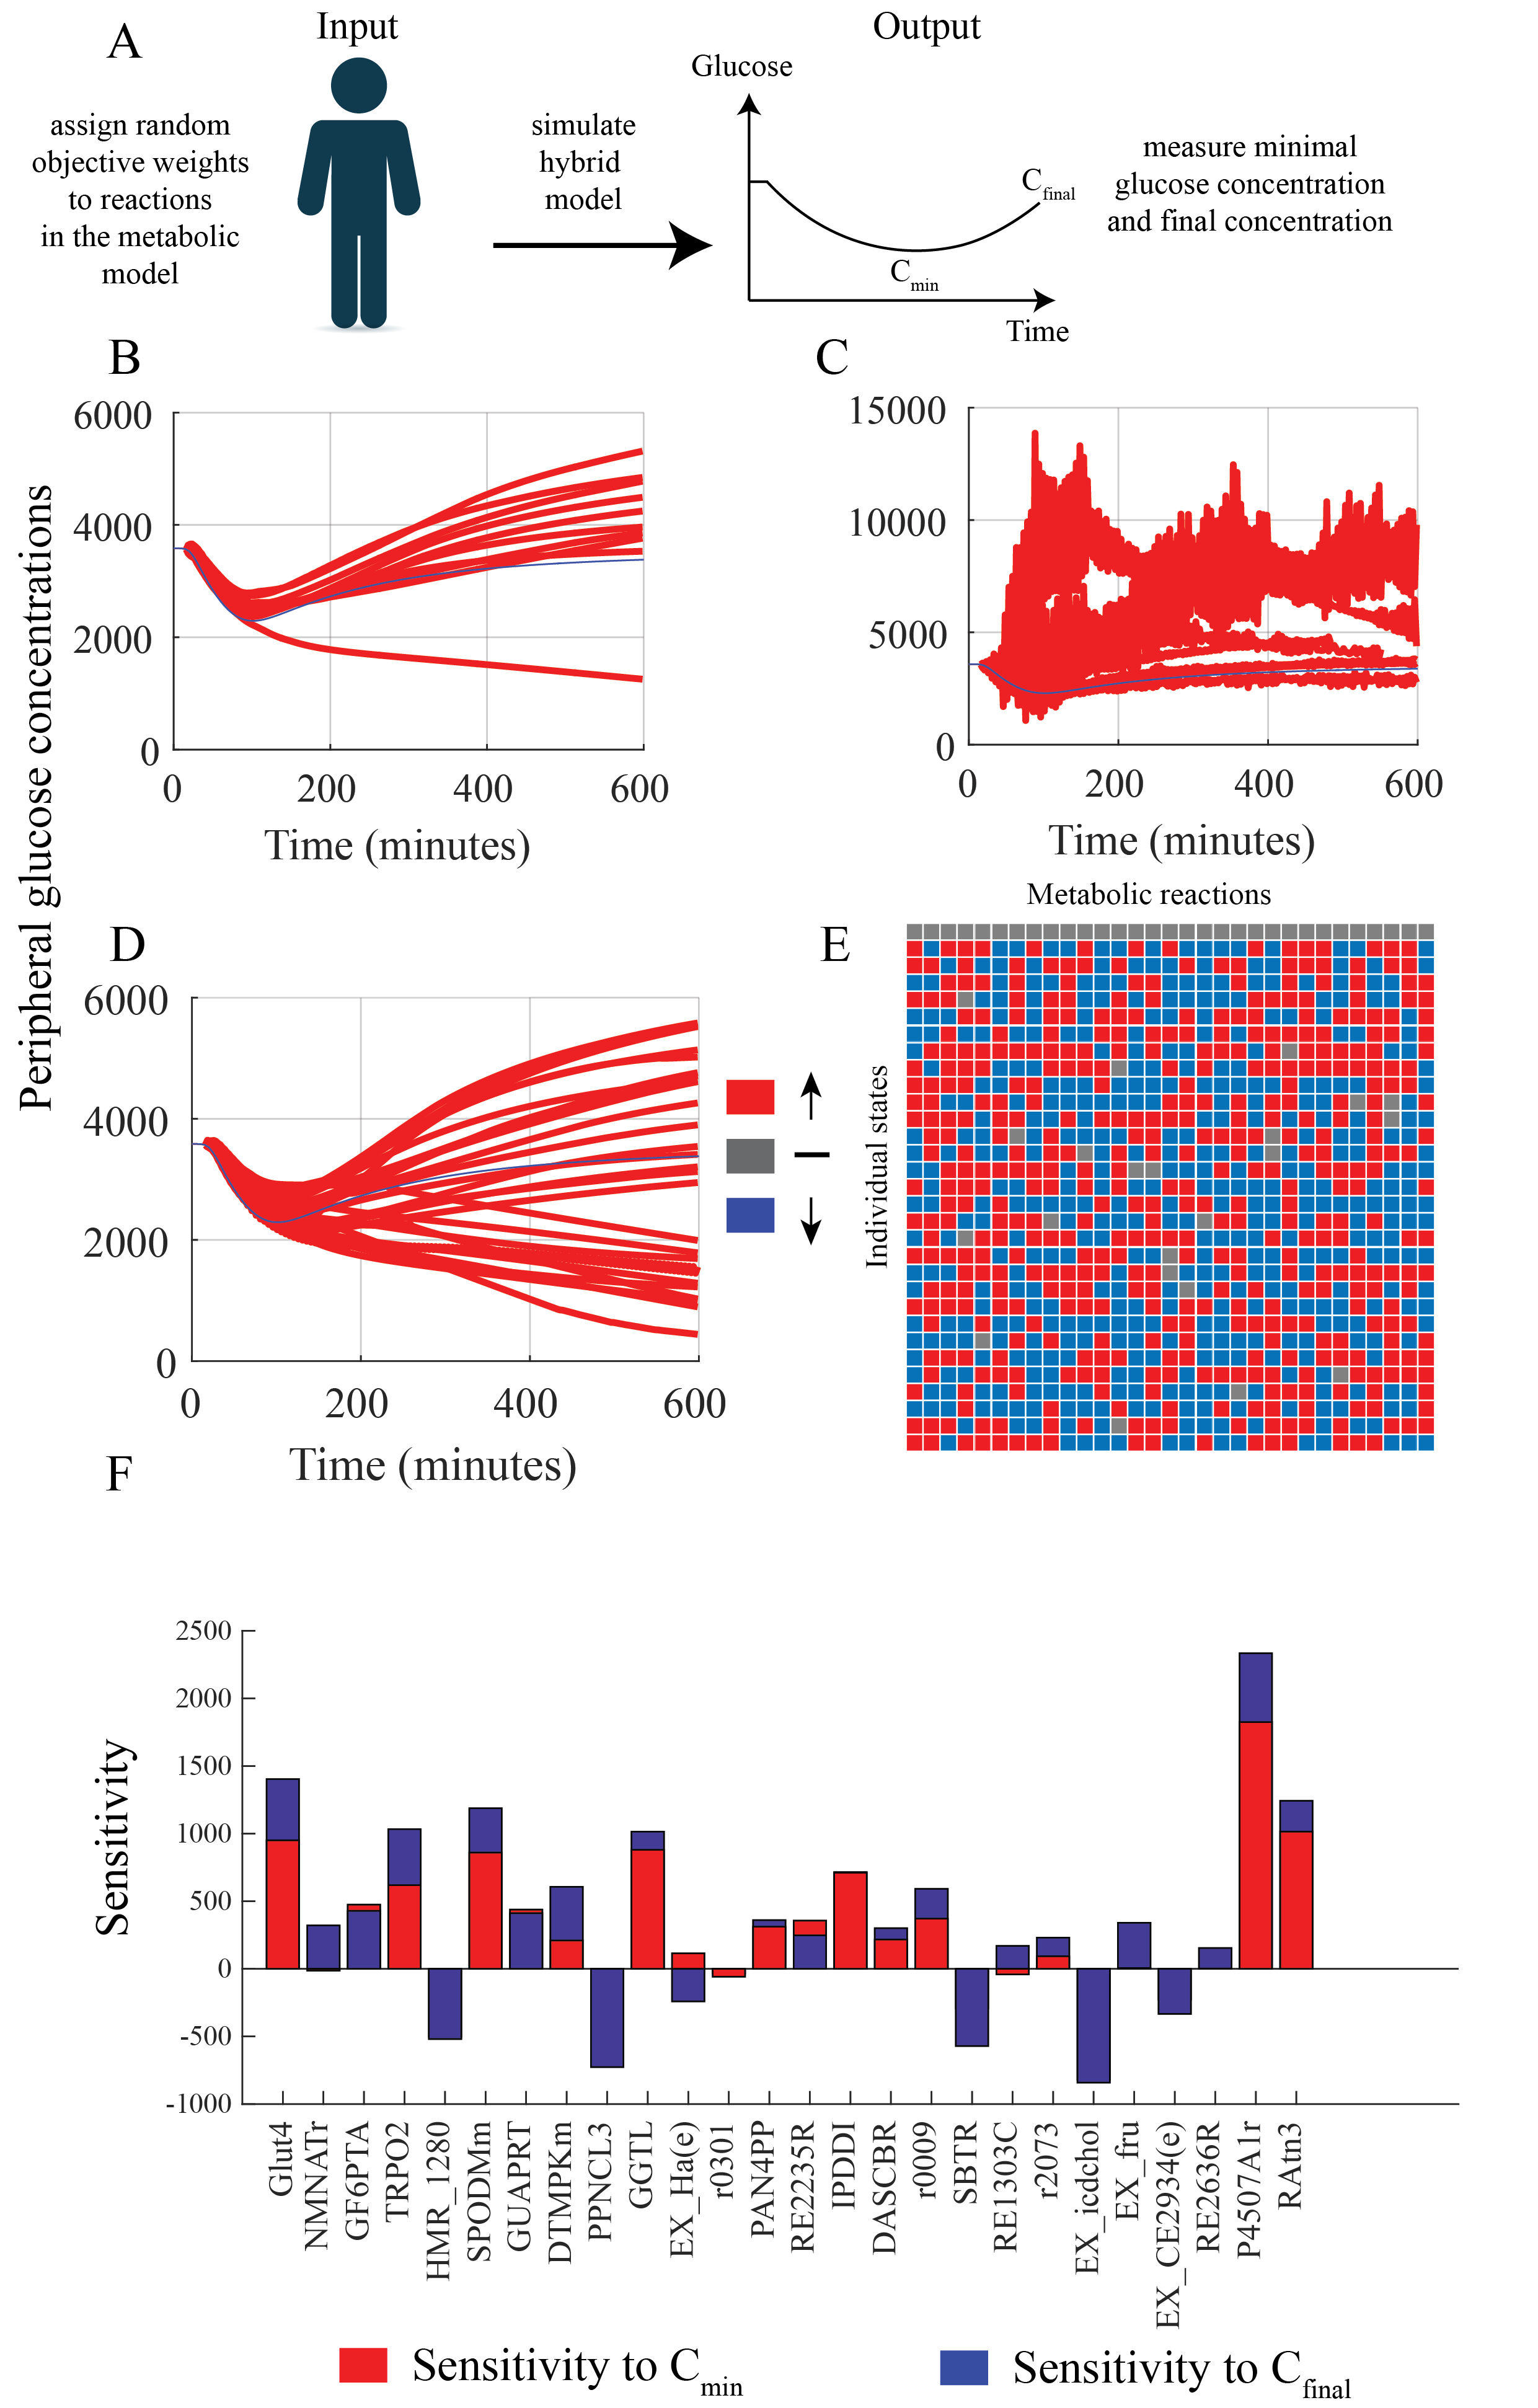
\includegraphics[width=\textwidth,height=\textheight,keepaspectratio]{GIM/figure5.png}%Figure from images\Figure1.png
	\caption[Intra-individual variability to insulin response.]{(Continued on the following page)}
	\label{fig:GIM5}
\end{figure}
\begin{figure}[t]
  \contcaption{Intra-individual variability is assessed through sensitivity analysis of the integrated model. A- The method consists of assigning random objective coefficients to metabolic reactions and measuring the minimal and final concentration of glucose for every state with the kinetic parameters set for the population mean. B-Peripheral glucose profile when only the interface reactions are varied, the simulation is carried with FBA (n=11). C-Glucose profile when both the interface reactions and the metabolic model reactions are varied, using FBA (n=11). D-Glucose profile when both the interface reactions and metabolic model reactions are varied, using CRONICS (n=31). E- A 31-column excerpt of the matrix of variation of reaction weights in the objective for every state. The total number of reactions considered was 2817. F- Computed sensitivities of every reaction in the internal state to the external output (minimal and final concentration of peripheral glucose). The reactions are described in table \ref{GIM:tblsRxn}.}% Continued caption
\end{figure}
We used gene expression data from type 1 diabetic pancreatic islets as constraints to represent the pathophysiology of the disease that associated both the chronic inflammation and the disruption of glycolytic processes. The total number of metabolic reactions in T1D was the same in the healthy model as no evidence suggested complete metabolic gene knockout in affected patients. dHarvey predicted a decrease in ATP in adipocyte (Figure \ref{fig:GIM2}-B) following the IVGTT test as glycogen storage pathways are activated over ATP producing pathways. 
Significantly  decreased pathways in T1D encompass mostly transport pathways in relation with the pan-organ distribution of insulin and the systemic properties of the disease. The well-known switch to fatty acid synthesis in type 1 diabetes is demonstrated in enrichment of the corresponding pathways (Figure \ref{fig:GIM2}-E). The up-regulation of sphingolipids, has been linked in particular to a decrease in tissue insulin sensitivity \cite{russo2013sphingolipids} in metabolic disorders and obesity.\\
Interestingly, tyrosine metabolism is significantly ranked in the up-regulated processes in T1D (Figure \ref{fig:GIM2}-E), and recent studies have found direct links between diabetes and tyrosine pathway disruption \cite{ferguson2013tatn}. Additionally, the alteration of the phosphoinositide metabolism was reported in a streptozotocyin-induced diabetes in platelet cells \cite{jethmalani1994platelet}. 
Moreover, the glycosaminoglycan family (chondroitin, keratin sulfate and N-glycan) which include naturally occurring molecules maintaining the tissue and cartilage, are decreased in T1D and could be at the origin of long-lasting manifestations such as the well-known disruption of tissue structure, e.g., diabetic foot. A study in rats showed a decrease of chondroitin sulfate in the kidney suggesting a possible implication in diabetes induced nephropathy \cite{joladarashi2011diabetes}. Collectively, the down-regulation of tissue remodeling pathways adds further evidence to the observed eschar-related symptomatology in diabetes. Since these manifestations happen at later stages, the tissue remodeling pathway \cite{gowd2016glycosaminoglycan} could be considered for interventional (either allopathic or nutritional) targets in the diagnosis phase.\\
The enrichment of genes associated to the increased fluxes in T1D (Table \ref{GIM:tbls2}) showed a representation of classical pathways such as the oxidative phosphorylation and carbon metabolism and, interestingly, Alzheimer's disease (AD), and Parkinson's disease were found to have potential common links to T1D (Table \ref{GIM:tbls5}, Figure \ref{fig:sx2GIM}). This finding further supports the growing evidence \cite{lalic2008glucose,moran2015type} for the common pathogenesis between neurodegenerative disorders and late-stage diabetes. Added to the comorbidities, up to 70\% of diabetic patients experience a cognitive decline \cite{cukierman2005cognitive}. Furthermore, a clinical trial repurposed Exenatide, a glucagon-like peptide-1 (GLP-1), indicated for the treatment of type 2 diabetes, in Parkinson's disease \cite{aviles2013exenatide,aviles2014motor}. Following the success of the early phases, a randomised double-blind trial \cite{athauda2017exenatide} showed that better motor functions were achieved at 48 weeks in comparison to a placebo, possibly in relation to insulin signalling pathways. In AD, a study showed that higher plasma and brain glucose levels were implicated in the disease progression \cite{an2017evidence} and the severity of the pathology. The increase in brain glucose levels was linked to a decrease in GLUT3 neuronal transporter expression and a reduced brain glycolytic flux, possibly explaining the comorbidities between AD and diabetes \cite{sims2010does,janson2004increased}.  Similarly, anti-diabetic drugs were suggested in AD \cite{guney2016network,yarchoan2014repurposing}, particularly GLP-1 agonists and glucagon that conferred neuroprotective effects and reversed memory loss in AD rodent models \cite{tai2018neuroprotective}. Among the small molecules that we found to revert the expression of genes associated to both the increased and decreased fluxes, Mibefradil and Amlodipine had a very good coverage (Table \ref{GIM:tbls6}). Encouragingly, studies in experimental rodent models of diabetes have shown that calcium blockers improved blood glucose levels and diabetes-associated nephropathy \cite{ma2004calcium, lu2014mibefradil}.\\
Taken together, these findings suggest the existence of a continuum between diabetes and neurodegenerative disorders, possibly involving a strong metabolic component.
\subsection{Insulin rewires inter-organ exchange}
Conceptually, dHarvey added the dynamic features of GIM to the genome-scale metabolic model Harvey, enabling a hybrid approach to metabolism. While GIM accurately predicted the glycolytic and regulatory effects of insulin, it could not capture the decrease of amino acids in the blood and other well-known anabolic effects \cite{dimitriadis2011insulin}. The addition of a dynamical model of insulin off-target effects \cite{yugi2014reconstruction} accurately predicted several known non-glycolytic effects of insulin (Figure \ref{fig:GIM3}). In  particular, the prediction of the triglycerides time-course (Figure \ref{fig:GIM3b}) using CRONICS, showed an increase in the adipocytes as a result of the inhibition of lipases. Furthermore, we predicted the effects of insulin on metal homeostasis as they play a prominent role in developing injection shocks due to the fast depletion of phosphate and potassium. Phosphate and potassium showed a trend towards an increase in the uptake, although these results are not conclusive (Figure \ref{fig:GIM3}). Given the great implication of those ions in signaling pathways, and the demonstrated insulin-induced signalling modulation \cite{yugi2014reconstruction}, signaling pathways might play a greater role than metabolism in the ions homeostasis. Given the small occurring concentrations of the ions in comparison to larger molecules, metabolism alone does not capture the full spectrum of micronutrient homeostasis.\\
Finally, to study the effect of insulin on inter-organ crosstalk, a subset of the reactions was selected to encompass the kidneys, liver, brain, pancreas, muscle, adipocyte, and inter-organ compartments, e.g., plasma, as the role of these organs have been demonstrated in the disease pathology \cite{li2009organ, romacho2014adipose}. The total inter-organ crosstalk increased as an effect of insulin administration (Figure \ref{fig:GIM3c}), further structuring the organs as a metabolic continuum. Multiple organ complications related to late-stage diabetes corroborates this finding as the loss of insulin mediates a decrease in organ crosstalk at a metabolic level. 
Although the implications of endocrine secretions have been more studied in systemic organ failure in pathology \cite{li2009organ}, the overall decrease in organ crosstalk in T1D might be a combined effect of the signalling and metabolic properties of insulin. 

\subsection{Insulin-mediated hysteresis reflects between-subject variability}
The generation of a synthetic population of T1D patients involved the variation of patient-specific kinetic parameters \cite{schaller2013generic}. The obtained peripheral glucose profile reproduced the reported 25\%-35\% of inter-individual variability to insulin and the differences were particularly noticed on the AUC, Cmin and Tmin (Figure \ref{fig:GIM4}-A,B). Interestingly, the patients had a similar number of active reactions, reflecting a similar network topology (Figure \ref{fig:GIM4}-C) which was also an effect of the simulation framework CRONICS that ensured a sparse set of fluxes and a minimal change between the time steps. This observation implies also the similar constitutive metabolic background between the patients and a conservation of the high-flux backbone \cite{almaas2004global}, in the absence of specific enzyme deficiency as in the case of IEMs \cite{sahoo2012compendium}. Although, when projecting the principal components of the flux distribution of individual patients during the simulation time, a metabolic shift could be observed. Two main results were subsequently deducted, first, the differences in response to insulin lie mainly in the modulation of flux values in the metabolic model (Figure \ref{fig:GIM4}-D) rather than the network structure. Second, the final metabolic state is different from the initial state, although the simulation time was large enough (10h) to ensure a return to steady state in the GIM model uncoupled to Harvey, which was consistent  with profound insulin-induced regulatory mechanisms on metabolism. Each patient achieved a differential control of the metabolic shift which can be related to the varying metabolic outcomes (Figure \ref{fig:GIM4}-E). In particular, insulin as indirectly represented by the glucose peripheral levels, induced a hysteresis in metabolism (Figure \ref{fig:GIM4}-F) which denotes the dramatic metabolic changes of insulin administration. In fact, the binding of insulin to its receptor and the release of GLUT transporters that has a ~15h half-life under insulin treatment \cite{sargeant1993effect} could be key drivers of the shift of the metabolic steady state, given the ubiquitous distribution of insulin receptors. Moreover, the hysteresis reflected the correspondence of several internal  metabolic states to a unique glucose concentration (Figure \ref{fig:GIM4}-F). This finding corroborates the unreliability of plasma glucose levels as a universal marker for the diagnosis of diabetes \cite{bonora2011pros}. \\
Additionally, the observed hysteresis revealed a differential action of insulin in the population, where in most patients it described a quasicycle between glucose concentrations predicted by GIM and the internal system properties modelled by the whole-body metabolic fluxes. It is noteworthy that a few patients did not achieve a metabolic shift and remained at the initial state, denoting ineffective insulin action, while a great distance of the final state could be a marker of hypo- or hyper-glycaemia and uncontrolled diabetes. \\
Finally, as hypothesized, the values of metabolic fluxes rather than network structure were the driver of the observed differences between the patients (Figure \ref{fig:GIM4}-G). In particular, the citric acid cycle and oxidative phosphorylation were supporting the observed between-subject variability while glycolysis and pentose phosphate pathways were robust to perturbation, denoting their essential role in human metabolism. In the architecture of metabolism, glycolysis and pentose phosphate pathways are at central position, while citric acid cycle and oxidative phosphorylation are the entry points to several secondary redundant pathways. In fact, external network nodes tend to act as buffers to absorb the perturbations and maintain the central functionalities of the network \cite{gilarranz2017effects}.\\
Taken together, the reduction of inter-individual variability in the response to insulin  is key to achieving diabetes control. Particularly, a study including a cohort of 20,303 individual \cite{akirov2017high}, showed that a higher coefficient of variance of glucose dynamics in diabetic patients was correlated to higher mortality rates, therefore, reducing within-patient variability is additionally a major determinant the management of T1D.
\subsection{GLUT4 as a pharmacogenomics target for diabetes control}
Within-patient variability to insulin poses a great challenge for the identification of the internal factors that could modulate the dynamics of glucose. Assuming the same kinetic parameters to represent the average patient, we randomly generated several internal metabolic states and consequently measured the glucose time series after insulin administration. Each state assumed different objective weights of a selected set of reactions. Moreover, CRONICS ensured the smoothness of the simulated system, wherein the outcome of the constraint-based model determined the dynamics of glucose, in contrast to the simulation setting of the inter-individual variability. The outcome of the simulation was in agreement with empirical intra-individual variability to insulin \cite{heinemann2002variability} and subsequently, the reactions were classified by their sensitivity to the final and the minimal glucose concentration, which acted as surrogate endpoints for insulin activity (Figure \ref{fig:GIM5}-F). 
%Expectedly, the reactions that were present in both Harvey and GIM modulated glucose dynamics (Figure \ref{fig:GIM5}-F). 
%Regarding metabolic reactions that are proper to Harvey, determining their sensitivities to glucose dynamics translated to computing their influence on interface reactions, which in return act directly on glucose dynamics. 
Given the high computational cost of the operation, we randomly selected representative reactions from each subsystem in all organs. The bile acid synthesis pathway was found to highly modulate glucose concentrations in the model. Particularly, studies have shown that dysregulation of the pathway could contribute to the pathogenesis of diabetes through the modulation of GLP-1 and insulin sensitizing activities \cite{prawitt2011bile,tomkin2016obesity}\\
Additionally, the transporter GLUT4 had a high sensitivity towards the minimal and final glucose concentration. The insulin-dependent carrier is released to balance high glucose concentrations and its expression could be a major factor of the pharmacodynamics of insulin \cite{correa2013slc2a4}. Generally, the transport subsystem, mediated by carrier proteins, provides a rationale for the design of novel antidiabetic drugs targeting transport proteins such as SGLT-1 \cite{sands2015sotagliflozin} and SGLT-2 \cite{verma2017metabolodiuretic}. 
Finally, since the flux through the GLUT4 reactions highly modulated glucose concentrations in the dHarvey model, we hypothesize that the carrier could be a major pharmacogenomics effector of insulin action. The design  of adjuvant therapy to insulin, targeting the expression and release of GLUT4 is a potential avenue to decrease intra-individual variability to insulin, overcome insulin resistance, and ultimately achieve diabetes control. Overall, the model presented in this study expands our understanding of type 1 diabetes and has the potential to empower evidence-based approaches to human pathology.

\section*{Acknowledgements}
The authors would like to acknowledge Bayer Technology Services for providing an academic version of PKSIM/MOBI software suite and providing the source file for the GIM model, Mr. Katsuyuki Yugi at the University of Tokyo for providing the insulin model as well as the Molecular Systems Physiology lab members at the University of Luxembourg for reviewing the manuscript.%Path to chapter

\chapter{Concluding remarks}
\label{ch:chapter6}
\chaptermark{Concluding remarks}%Short description for page header
Genome-scale metabolic models have been widely used to reconstruct bacterial organisms  \textit{in silico} and to simulate their phenotype in different media. The end goal is to accumulate as much information as possible to obtain models that resemble the actual organisms and are entirely predictive of their capacity. Genome-scale metabolic models are knowledge-bases of metabolism and as such they are built in a hypothesis-free manner and used to interrogate the model for a set of questions. ODE-based dynamical models are smaller in coverage of biological process although they harbour crucial dynamical properties that can further characterize the organism in time and space. The dynamical models are poorly scalable and are usually hypothesis-driven, which means that they are built in order to answer a specific question at a specific time. As I detailed in the introduction, building hybrid models of metabolism using both ODE-based models and  steady-state genome-scale models, can leverage the advantages of both types of models to increase the accuracy and scope of predictions. Although, a question that hasn't been brought up enough in the community surrounds the compatibility of these modeling techniques. Is the hybrid model hypothesis-free or hypothesis-driven? Is the model valid for all time, in all conditions or does it live for a short period of time to answer a specific question? What is the compromise in time interval for a biological system to achieve steady-state and meet the integration tolerance of ODEs? Is the model the smallest set of equations that better describe the data? Do the steady-state constraints apply in short-time dynamics?.\\
Answering these questions is crucial to properly assess the range of action of hybrid models. 
%For example, using economical models outside their application conditions drove austerity policies in countries that did not apply, thereby affecting the lives of millions of people \cite{leigh2013growth}, let alone biomedical and clinical trial models.
\section{Constraining dynamical models, how much is enough?}
Coupling dynamical ODE-based models and genome-scale metabolic models, requires points of intersection in metabolites or reactions. Oftentimes, the intersection set is a small set in comparison to the size of the metabolic model. Then we can legitimately ask if the changes induced by the intersecting set are enough to induce a whole-system shift in metabolism and to drive a dynamic change in phenotype, dictated by the dynamical model. In the first coupled model of Ecoli \cite{covert2008integrating}, the authors coupled all available reactions and metabolites in the dynamical model to the genome-scale model. In return the genome-scale model informed the ODE model with new rates specific to the biomass. The coupled model provided closer results to the experimental data than each of the model on their own. Later in the first model combining PBPK and genome-scale models \cite{krauss2012integrating}, the intersection points were only two reactions, namely the organ perfusion and the organ secretion for allopurinol, which matched the uptake and secretion reactions in the genome-scale model. We used a similar approach to predict the pharmaockinetics of levodopa with a set of diets (\hyperref[ch:chapter3]{Chapter 3}). Two matching reactions here are enough to predict the concentrations of allopurinol, because in PBPK models, the concentrations are entirely determined by in and out rates. In another work \cite{tummler2015dynamic}, a dynamical model has been embedded into a genome-scale model, to backtrack the contribution of metabolites to the biomass, which allowed to correct the predictions of the dynamical model using species that were not initially included in the ODEs.\\
So to the question 'How many dynamical constraints should I apply to the genome-scale model?' my answer would vary with the question sought. It stays obvious that a large number of constraints involving key processes like the biomass and imbalanced reactions are drivers of metabolic shifts in large-scale metabolic models. If the question surrounds the prediction of the concentration of a specific set of metabolites then coupling reactions directly involved in their anabolic and catabolic processes is sufficient, independently of the original size of the model.\\
Equally, achieving steady state is a central assumption in genome-scale metabolic models and forms the basis for Flux Balance Analysis (FBA). In this case, the rate-of-change of metabolites is zero, while dynamical models allow to obtain the time-course of metabolites through integrating ODEs. Then what should be the stand of a hybrid model towards the steady-state assumption? The allopurinol combined PBPK and genome-scale liver model \cite{krauss2012integrating} addressed this issue through maintaining the steady-state assumption and performing the coupling on the imbalanced reactions. The imbalanced reactions in a genome-scale model are exchange or biomass reactions whose rate-of-change is not equal to zero. As a matter of fact, the steady-state assumption in genome-scale models is only partial and includes only internal metabolites. In the hybrid model of E.coli \cite{covert2008integrating}, the authors lifted the steady-state assumption on internal metabolites whose rate-of-change is known by the dynamical model and kept the remaining metabolites as steady-state. Finally, the co-existence of steady-state and non-steady metabolites is mainly driven by the availability of data and has to be clearly communicated in the modeling phase as it could lead to confusion and misinterpretation.\\
How much should be the length of the time step between discrete and continuous dynamics? Most attempts so far have taken into account the integration tolerance as a main objective \cite{covert2008integrating,gomez2014dfbalab,hanly2011dynamic}. Then a recurrent question in field comes with regards to biological relevance: does the biological system optimize for short time steps or does it have an endpoint objective function? The former seems more concordant with experimental data although the latter is more intuitive \cite{mahadevan2002dynamic}.
\section{Tractability and model reduction}
Building a hybrid body-wide model of carbohydrate metabolism and regulation (Ben Guebila and Thiele, in preparation) posed a totally new set of questions that were triggered by the exceptional size of the model (> 80,000 reactions, > 10,000 ODEs). Maintaining a chronologically coherent set of predictions required the design of new tools (\hyperref[ch:chapter5]{Chapter 5}). Particularly, the size of the model made it largely under-determined, which required the selection of the solutions that are closer to the previous time step in a flip book analogy. This type of issues was not affecting small size model as the solution space is much reduced and usually the constraints from the dynamical model ensure the smoothness of the system. The downside of this addition was that it turned the simulations into time-critical operations. The simulation is in the order of days, which affects the development and re-use of this type of models as specific hardware is required.\\
Although this question came up newly in the field of metabolic modelling, I find that getting inspiration from aerospace modelling could be salutary. In the beginning of the race to space, the large simulation time of the shuttle trajectory reportedly delayed several missions \cite{phillips2005journey}.
Model reduction is based on a simple concept: first the building of the detailed mechanistic model and the simulation for a set of output variables. Although, the original model is rich in information and the length of simulation time makes it impracticable for real world needs e.g., space shuttle launch, clinical trials, as no one would wait for months to make a go/no-go decision. The problem is often referred to as the curse of parametrisation and is often dealt with through selecting an output variable of interest to the question. Second, model order reduction is performed through projecting it into a lower dimension after determining the main readout variable of the model \cite{zahr2017multilevel,amsallem2016real}. In its compact form the model can hold on a USB thumb-drive and can be exchanged and manipulated very fast to answer what-if type of questions.
The original rich system is usually sensitive to the initial conditions, it is then perturbed and sub-regions of solutions are identified, sampled, compressed and finally clustered to represent a set of output solutions \cite{balajewicz2016projection,farhat2016recent}. This means that for a small number of large-scale simulations, the behaviour of the system can be reduced to the informative regions.
%The design of stealth aircraft uses reduced models Petr Ufimtsev
%Model form incertainty.vs parametric uncertainity
\section{A regulatory perspective}
The increasing use of hybrid models in biomedical applications and particularly in pharmacometrics naturally brings a reflection on the regulatory aspect of modeling. The FDA has been accepting PKPD and PBPK models \cite{us2004innovation} to support labelling of products, the optimal design of clinical trials, drug-drug interactions, prediction of exposure in paediatric population, estimation of absorption, and as a support for regulatory review in general \cite{sager2015physiologically,pan2014application}. Recently, a closed-loop controlled insulin pump in T1D has been accepted without preclinical trials, using solely the model simulations \cite{kovatchev2009silico}. What would be the stand of the regulator towards hybrid models of continuous and discrete dynamics?\\
While PKPD models are the smallest models that best fit the data, this type of hybrid model is certainly not minimal. Constraint-based modeling is rather a semi-quantitative approach and is not as accurate as full dynamical models in predicting reaction rates. As such, the hybrid model is semi-quantitative, particularly for the metabolites and reactions that are covered by the genome-scale metabolic model alone. Hybrid models are certainly useful in preclinical trials, target discovery, and biomarker identification. In clinical trials, a large set of constraints are needed to constrain the hybrid model to the biologically relevant observations, such as the constraints provided by the GIM model that covers all the organs and a large number of processes. Nevertheless, the detail and scope of the GIM model make it certainly anecdotal, there are a handful of models that are equal in granularity and size. Particularly, to estimate the large number of kinetic parameters in PBPK models, concentration data in the target organs need to be measured to accurately estimate organ-specific rates of metabolism. Nevertheless, the use of organ diffusion models can provide an accurate estimation of the metabolised fraction \cite{rodgers2005physiologically,rodgers2006physiologically}. In order to perform classical pharamacometric analyses on large-scale models including bootstrapping of parameters, finding correlation between parameters, and mixed-effect non-linear population modeling, new mathematical tools have to be developed in order to meet the needs of the regulatory bodies, particularly through addressing parametric uncertainty and model-form uncertainty.\\
The increasingly accessible biological data combined with adequate open-source software such as PKSIM \cite{willmann2003pk}, will make it easier to build whole-body models, which can bring modeling in the forefront of clinical trials design.
\section{What is next? writing the ODE of life.}
Many view hybrid models of continuous and discrete dynamics as a a pitstop towards full dynamical models of biological systems. Recently, a few large-scale ODE systems of bacterial metabolism were developed \cite{khodayari2016genome,dash2017development}, equalling in size the first generation of constraint-based metabolic models. Dynamical models are certainly more adequate than constraint-based models in quantitatively answering specific questions with respect to the system dynamics, particularly when the uncertainty is quantified and assessed. Although seeing them as the ultimate goal of explaining life is certainly delusional. This is because of the large number of parameters to estimate, the different rate processes, the modeling of the different types of affinities and inhibitory processes,  and the \textit{in vivo} enzyme kinetics. While I think this goal is within reach in the upcoming years, I believe that smaller tractable models can provide an equally insightful result to a specific question at a given time and for a fraction of the development cost; to quote Von Neumann: 'If people do not believe that mathematics is simple, it is only because they do  not realize how complicated life is'.%Path to chapter
% References

\setstretch{1}%chose single space for references and supplements
\bibliographystyle{apalike}
\bibliography{references}

% Appendices
%
\appendix
\chapter{Supplementary material for Chapter 2}
\section{Supplementary tables}

\begin{table}[h]
\caption[Optimal classifier parameters]{Support vector machine parameter summary}
\begin{center}
	\begin{tabular*}{\textwidth}{l @{\extracolsep{\fill}} ll}
	\hline
	Parameter	                     & Optimal value/algorithm       \\ 
	\hline
	Feature selection algorithm     & ReliefF     \\
	k-ReliefF         & 80        \\
	Number of features                     & 20             \\
	Cross-validation       & 3-fold cross-validation          \\
	Class balance      & Inverse of class frequencies           \\
	Observation weights       & Drug side effect frequency per drug           \\
	SVM kernel       & Gaussian           \\
	\hline
	\end{tabular*}
\end{center}
\label{tbl:tbls1ch2}%descriptive label to refer to figure in text
\end{table}

\newpage

\begin{table}[h]
\caption[Automatically optimized SVM hyperparameters.]{Automatically optimized SVM hyperparameters.}
\begin{center}
	\begin{tabular*}{\textwidth}{l @{\extracolsep{\fill}} ll}
	\hline
	Hyperparameter	                     & Value/Range       \\ 
	\hline
	Standardize data     & True,false     \\
	Kernel         & Linear, Gaussian, polynomial        \\
	Polynomial order                     & [2,5]             \\
	Box constraints       & [1e-6,1e+4]         \\
	Kernel scale      & True,false          \\
	\hline
	\end{tabular*}
\end{center}
\label{tbl:tbls2ch2}%descriptive label to refer to figure in text
\end{table}

\newpage
\newpage

\begin{table}[h]
\caption[Area under the ROC curve of the predicted side effect.]{Area under the ROC curve of the predicted side effect using a multi-label support vector machine classifier with combined gene expression and sampled metabolic flux as features.}
\begin{center}
	\begin{tabular*}{\textwidth}{l @{\extracolsep{\fill}} ll}
	\hline
	Side effect	                     & AUROC       \\ 
	\hline
Gastrointestinal pain                 & 0.52\\
Gastrointestinal disorder             & 0.53\\
Functional gastrointestinal disorder  & 0.63\\                 
Gastrointestinal haemorrhage          & 0.64\\    
Intestinal obstruction                & 0.67\\     
Intestinal perforation                & 0.69\\  
Gastrointestinal tract irritation     & 0.72\\ 
Gastrointestinal perforation          & 0.74\\ 
Gastrointestinal obstruction          & 0.75\\   
Gastrointestinal fistula              & 0.79\\
Intestinal ulcer                      & 0.8\\   
Gastrointestinal hypomotility         & 0.8\\        
Gastrointestinal sounds abnormal      & 0.9\\ 
Gastrointestinal ulcer haemorrhage    & 0.9\\     
Gastrointestinal infection            & 0.91\\
Gastrointestinal necrosis             & 0.92\\ %%  
Gastrointestinal toxicity             & 0.92\\ 
Upper gastrointestinal haemorrhage    & 0.93\\ 
Lower gastrointestinal haemorrhage    & 0.95\\
Gastrointestinal carcinoma            & 0.96\\
Gastrointestinal ulcer perforation    & 0.96\\
Gastrointestinal motility disorder    & 0.97\\ 
Intestinal infarction                 & 0.97\\
Gastrointestinal ulcer                & 0.97\\
Gastrointestinal stromal tumour       & 0.97\\
Pneumatosis intestinalis              & 0.97\\           
Intestinal ischaemia                  & 0.98\\      
Large intestine polyp                 & 0.98\\ 
Gastrointestinal malformation         & 0.98\\ %%   
Gastrointestinal candidiasis          & 0.99\\   
Benign gastrointestinal neoplasm      & 0.99\\  
Gastrointestinal inflammation         & 0.99\\  
Diverticulum intestinal               & 0.99\\   
Large intestine perforation           & 0.99\\  
Small intestinal obstruction          & 0.99\\  
Intestinal haemorrhage                & 0.99\\  
	\hline
	\end{tabular*}
\end{center}
\label{tbl:tbls3ch2}%descriptive label to refer to figure in text
\end{table}

\clearpage
\section{Supplementary figures}
\begin{figure}[!htp]
\centering
	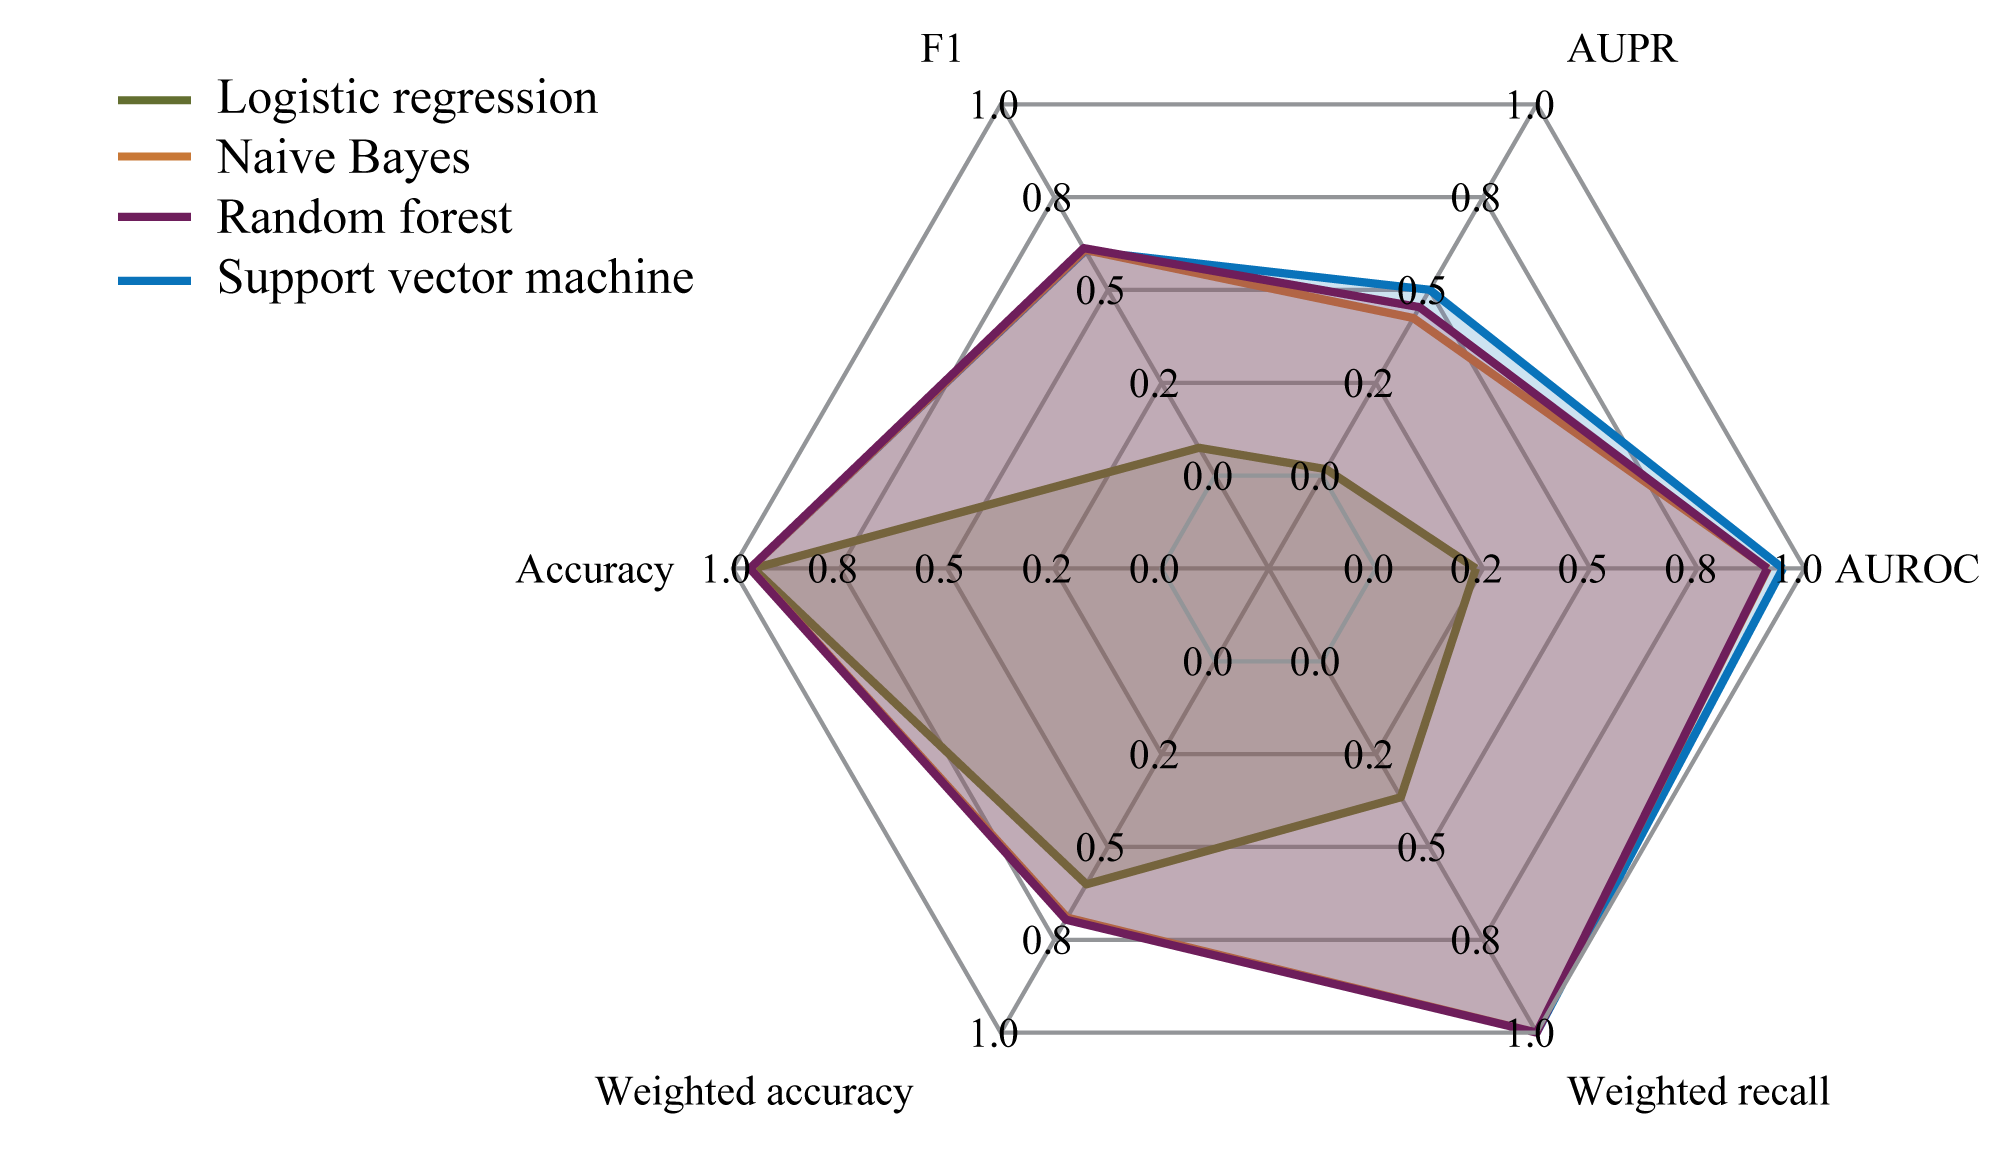
\includegraphics[width=\textwidth,height=\textheight,keepaspectratio]{sideEffects/Algorithms.png}%Figure from images\Figure1.png
	\caption[Comparison of multi-label classifiers.]{Comparison of multi-label classifiers. Four classifiers namely, logisitic regression, naive Bayes, random forest, and support vector machine were compared in their predictive capabilities measured by the F1-score, accuracy,class weighted accuracy, class weighted recall, area under the ROC curve (AUROC), area under the precision-recall curve (PR).}
	\label{fig:s1algo}
\end{figure}

\clearpage
\begin{figure}[!htp]
\centering
	\includegraphics[width=\textwidth,height=\textheight,keepaspectratio]{sideEffects/figS1.png}%Figure from images\Figure1.png
	\caption[Feature selection algorithm comparison.]{Comparison of 11 feature selection algorithm with respect to the area under the ROC curve of individual intestinal side effects with the 95\% confidence interval for the mean in red and one standard deviation in blue.}
	\label{fig:s1seff}
\end{figure}

\clearpage
\begin{figure}[!htp]
\centering
	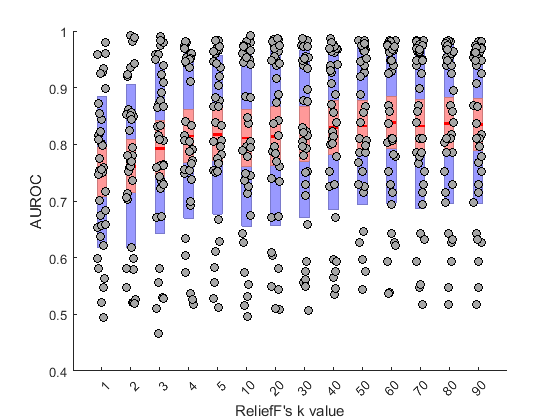
\includegraphics[width=\textwidth,height=\textheight,keepaspectratio]{sideEffects/figS2.png}%Figure from images\Figure1.png
	\caption[ReliefF's k value comparison.]{Comparison of k values for the feature selection algorithm ReliefF through the area under the ROC curve of classifiers of individual side effects with the 95\% confidence interval for the mean in red and one standard deviation in blue. The highest mean (0.83) was achieved for k=80.}
	\label{fig:s2seff}
\end{figure}

\clearpage
\begin{figure}[!htp]
\centering
	\includegraphics[width=\textwidth,height=\textheight,keepaspectratio]{sideEffects/figS3.png}%Figure from images\Figure1.png
	\caption[Comparison of the number of selected features.]{Comparison of the effect of the number of the most predictive features on the classification performance as assessed by the area under the ROC curve.}
	\label{fig:s3seff}
\end{figure}

\clearpage
\begin{figure}[!htp]
\centering
	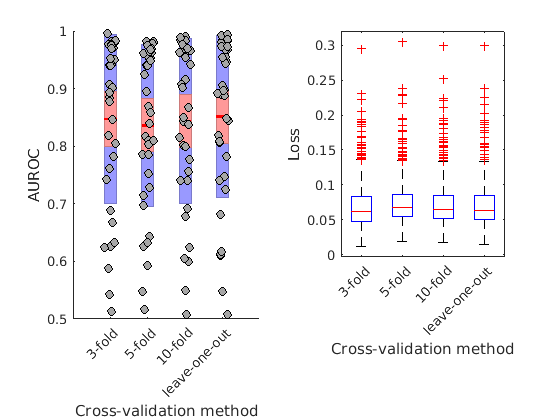
\includegraphics[width=\textwidth,height=\textheight,keepaspectratio]{sideEffects/figS4.png}%Figure from images\Figure1.png
	\caption[Assessment of the cross-validation loss.]{Comparison of cross-validation method on the loss computed as the number of misclassified side effects per drugs over the total number of side effects, and the predictability of the individual side effects as reflected by area under the ROC curve (AUROC). Outliers in the loss are rare side effects that have a small number of data points. The 3-fold cross-validation ensured a lower loss and the highest area under the ROC curve on out-of-sample drugs. Left: distribution of AUROC of individual side effects with the 95\% confidence interval for the mean in red and one standard deviation in blue. Right: boxplot of the loss computed for each cross-validation method.}
	\label{fig:s4seff}
\end{figure}

\clearpage
\begin{figure}[!htp]
\centering
	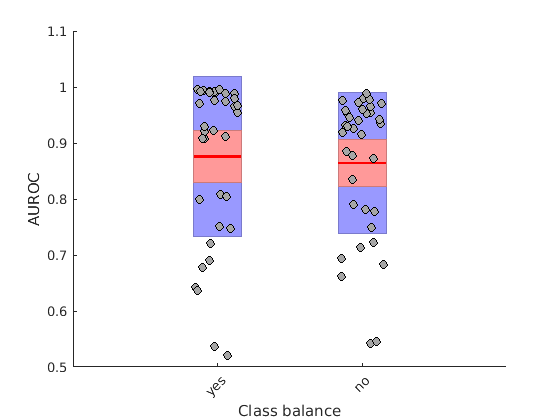
\includegraphics[width=\textwidth,height=\textheight,keepaspectratio]{sideEffects/figS5.png}%Figure from images\Figure1.png
	\caption[Effect of class balance.]{Comparison of the effect of class balance set as the misclassification cost, on the outcome of the classification as determined by the area under the ROC curve. The misclassification cost, set to the inverse of class frequencies, allowed to obtain a mean of 0.875 of the AUROC of the individual intestinal side effects as opposed to 0.86 without class balance.}
	\label{fig:s5seff}
\end{figure}

\clearpage
\begin{figure}[!htp]
\centering
	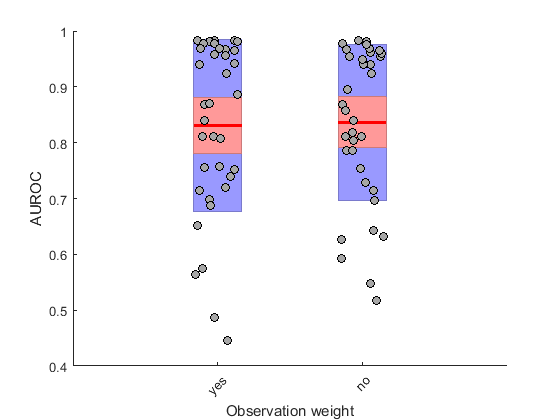
\includegraphics[width=\textwidth,height=\textheight,keepaspectratio]{sideEffects/figS6.png}%Figure from images\Figure1.png
	\caption[Effect of observation weight.]{Comparison of the effect of adding observation weights to the classifier as compared the area under the ROC curve. The weights of drugs per class were set to their frequencies reported in SIDER. Weighing observations has a mean area under the curve of 0.830 while unweighted observation has a mean of 0.836.}
	\label{fig:s6seff}
\end{figure}

\clearpage
\begin{figure}[!htp]
\centering
	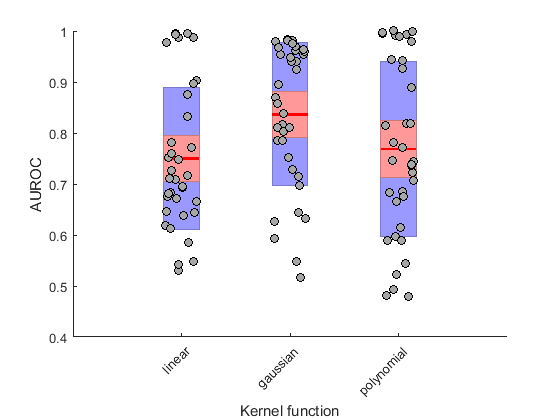
\includegraphics[width=\textwidth,height=\textheight,keepaspectratio]{sideEffects/figS7.png}%Figure from images\Figure1.png
	\caption[Comparison of SVM kernel functions.]{Comparison of SVM kernel functions as a function of area the under the ROC curve of individual side effects. Over all, the Gaussian kernel had the highest predictive capabilities.}
	\label{fig:s7seff}
\end{figure}

\clearpage
\begin{figure}[!htp]
\centering
	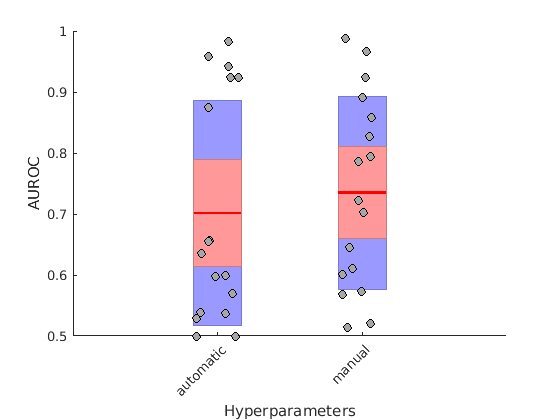
\includegraphics[width=\textwidth,height=\textheight,keepaspectratio]{sideEffects/figS8.png}%Figure from images\Figure1.png
	\caption[Automatic tuning of kernel parameters.]{Effect of automatic and manual hyperparameter optimisation with respect to 20\% holdout accuracy as an objective function. The manually obtained parameters allowed for a higher predictive capability of the classifier as measured by the individual side effect area under the ROC curve.}
	\label{fig:s8seff}
\end{figure}

\clearpage
\begin{figure}[!htp]
\centering
	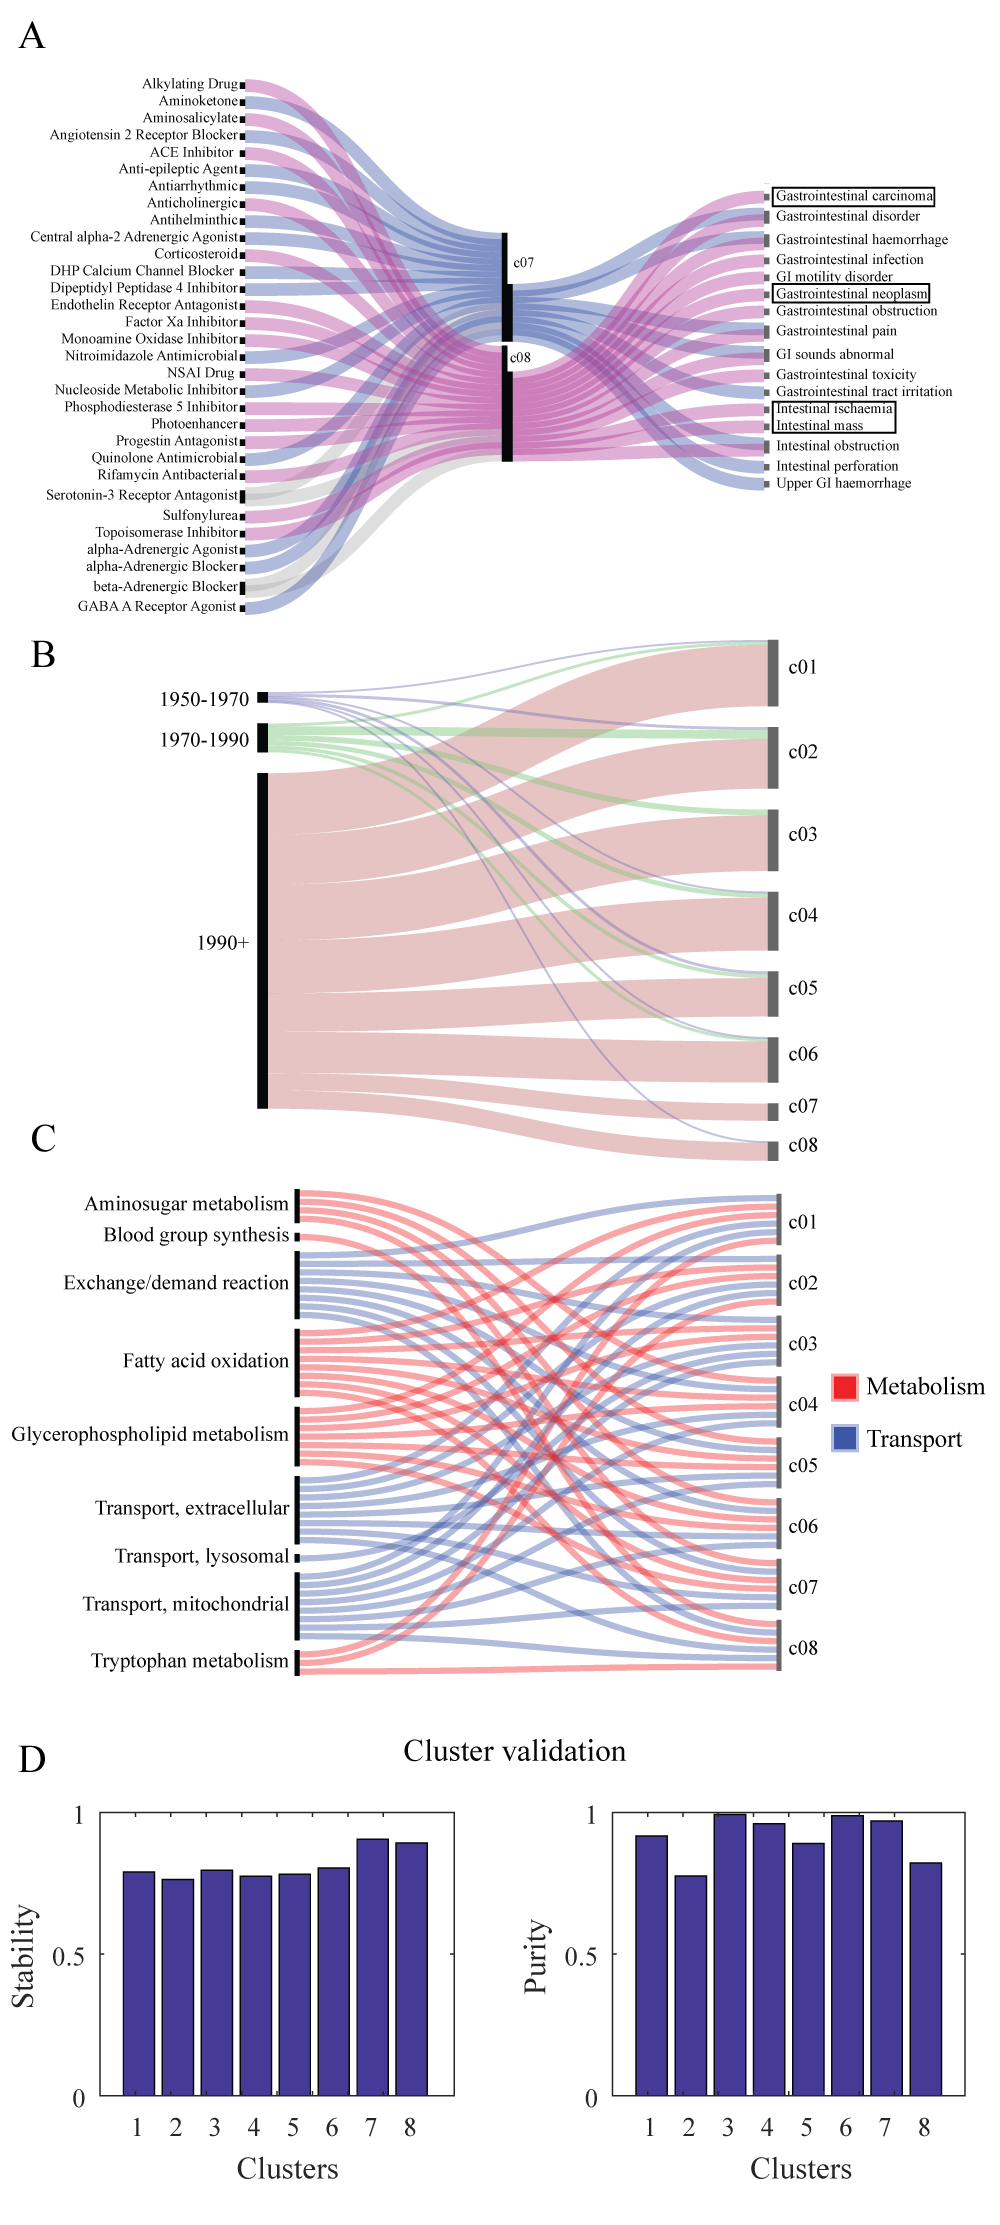
\includegraphics[width=\textwidth,height=\textheight,keepaspectratio]{sideEffects/figS9.png}%Figure from images\Figure1.png
	\caption[Drug cluster validation and characteristics]{(Continued on the following page)}
	\label{fig:s9seff}
\end{figure}
\begin{figure}[t]
  \contcaption{Drug cluster validation and characteristics. A- Graph linking drug clusters, intestinal side effects and FDA NDCD’s established pharmacological class (EPC). B- Bipartite graph of drug clusters and the corresponding FDA NDCD’s reported marketing date. C-Bipartite graph of drug clusters and enriched metabolic and transport subsystems. The flow chart was done using Rawgraphs \cite{Mauri:2017:RVP:3125571.3125585}. E-Cluster stability and purity provided a means for cluster validation.}% Continued caption
\end{figure}
%Path to supplementary material

\chapter{Supplementary material for Chapter 3}
\section{Supplementary tables}
The following table are too large to be displayed in text and are available via the publisher's website.

\begin{table}[h]
\caption[Ordinary differential equation-based levodopa pharmacokinetics.]{\hbox{Table of Ordinary differential equation-based levodopa pharmacokinetic model.}\\\hbox{Direct download: }\href{https://images.nature.com/original/nature-assets/npjsba/2016/npjsba201613/extref/npjsba201613-s2.doc}{\hbox{https://images.nature.com/original/nature-assets/npjsba/2016/npjsba2016}\\13/extref/npjsba201613-s2.doc}}
\begin{center}
	\begin{tabular*}{\textwidth}{l @{\extracolsep{\fill}} ll}
	\hline
	Columns	                     & Description       \\ 
	\hline
	Equation name     & The name of the current equation in the model.     \\
	Equation description         & A detailed description of the biological process associated\\ & to the equation.        \\
	Equation                     & The formal ODE.             \\
	Parameter description        & A description of the biological relevance of the equation's\\ & parameters.           \\
	\hline
	\end{tabular*}
\end{center}
\label{tbl:tbls1}%descriptive label to refer to figure in text
\end{table}

\newpage
\begin{table}[h]
\caption[Whole-body generic PBPK model parameter estimation from curve fitting.]{\hbox{Table of whole body generic PBPK model parameter estimation from curve fitting.}}
\begin{center}
	\begin{tabular*}{\textwidth}{l @{\extracolsep{\fill}} llll}
	\hline
	Parameter  	                      & Model constraints & Estimated value & Literature value       \\ 
	\hline
	Molecular weight                  & 197.18 g/mol & Fixed & 197.18 g/mol \cite{knox2010drugbank}    \\
	\makecell[l]{Blood plasma\\ partition coefficient}         & > 0 & 0.57 & -       \\
	Clearance                         & 0.5-5 l/kg/h & 0.95 l/kg/h & 0.55-1.38 l/kg/h \cite{martinelli2003levodopa}         \\
	Log of permeability               & < 0 & -4.9 & -2.39          \\
	Unbound fraction                  & 0.6-0.95 & 0.95 & 0.6-0.95 \\
	\makecell[l]{Effective luminal \\ intestinal permeability} & 0-5 cm/hour & 1.8 cm/hour & 1.22 cm/hour \cite{lennernas1993effect}  \\
	Distribution factor               & > 0 & 1.24 & - \\
	\makecell[l]{Effective basolateral\\ intestinal permeability} & 0-5 cm/hour & 3.6 cm/hour & \makecell[l]{$\geq$ Effective luminal \\ intestinal permeability \cite{agoram2001predicting}} \\
	\hline
	\end{tabular*}
\end{center}
\caption*{The estimated parameters are within the reported biological interval. The clearance regroups the overall elimination from the body in the eliminating organs (brain, kidneys, liver). The parameters units are mentioned and dimensionless otherwise.}
\label{tbl:tbls2}%descriptive label to refer to figure in text
\end{table}

\newpage
\begin{table}[h]
\caption[Reactions added to the sIEC model ordered by affinity of amino acids to the corresponding transporter.]{Reactions added to the sIEC model ordered by affinity of amino acids to the corresponding transporter.}
\begin{center}
	\begin{tabularx}{\textwidth}{L{10.5cm}L{4cm}}
	\hline
	\textbf{Luminal antiport reactions}        & \textbf{GPR(Entrez ID)}     \\ 
	\hline
	34dhphe[u] + ala\_L[c] $\rightarrow$ 34dhphe[c] + ala\_L[u] &    \\
	34dhphe[u] + leu\_L[c] $\rightarrow$ 34dhphe[c] + leu\_L[u] & 11136 and 6519 \cite{verrey2000glycoprotein}   \\
	34dhphe[u] + leu\_L[c] $\rightarrow$ 34dhphe[c] + leu\_L[u] &        \\
	\hline
	\end{tabularx}\par\vskip-1.4pt
		\begin{tabularx}{\textwidth}{L{10.5cm}L{4cm}}
	\hline
	\textbf{Basolateral antiport reactions}        & \textbf{GPR(Entrez ID)}     \\ 
	\hline
	34dhphe[c] + tyr\_L[e] $\rightarrow$ 34dhphe[e] + tyr\_L[c] &    \\
	34dhphe[c] + trp\_L[e] $\rightarrow$ 34dhphe[e] + trp\_L[c] &    \\
	34dhphe[c] + phe\_L[e] $\rightarrow$ 34dhphe[e] + phe\_L[c] &     \\
	34dhphe[c] + thr\_L[e] $\rightarrow$ 34dhphe[e] + thr\_L[c] &    \\
	34dhphe[c] + ile\_L[e] $\rightarrow$ 34dhphe[e] + ile\_L[c] &    \\
	34dhphe[c] + cys\_L[e] $\rightarrow$ 34dhphe[e] + cys\_L[c] &  23428 and 6520 \cite{verrey2000glycoprotein}   \\
	34dhphe[c] + ser\_L[e] $\rightarrow$ 34dhphe[e] + ser\_L[c] &    \\
	34dhphe[c] + val\_L[e] $\rightarrow$ 34dhphe[e] + val\_L[c] &    \\
	34dhphe[c] + leu\_L[e] $\rightarrow$ 34dhphe[e] + leu\_L[c] &     \\
    34dhphe[c] + glu\_L[e] $\rightarrow$ 34dhphe[e] + glu\_L[c] &    \\
	34dhphe[c] + ala\_L[e] $\rightarrow$ 34dhphe[e] + ala\_L[c] &    \\
	34dhphe[c] + his\_L[e] $\rightarrow$ 34dhphe[e] + his\_L[c] &     \\
    34dhphe[c] + asp\_L[e] $\rightarrow$ 34dhphe[e] + asp\_L[c] &    \\
	34dhphe[c] + met\_L[e] $\rightarrow$ 34dhphe[e] + met\_L[c] &    \\
	\hline
	\end{tabularx}\par\vskip-1.4pt
	\begin{tabularx}{\textwidth}{L{10.5cm}L{4cm}}
	\hline
	\textbf{Complementary luminal amino acids}        & \textbf{GPR(Entrez ID)}     \\ 
	\textbf{antiport reactions} & \\
	\hline
	leu\_L[u] + ala\_L[c] $\rightarrow$ leu\_L[c] + ala\_L[u] &    \\
	leu\_L[u] + arg\_L[c] $\rightarrow$ leu\_L[c] + arg\_L[u] &    \\
	lys\_L[u] + arg\_L[c] $\rightarrow$ lys\_L[c] + arg\_L[u] &    \\
	lcystin[u] + arg\_L[c] $\rightarrow$ lcystin[c] + arg\_L[u] & 11136 and 6519 \cite{verrey2000glycoprotein}   \\
	orn[u] + arg\_L[c] $\rightarrow$ orn[c] + arg\_L[u] &    \\
	tyr\_L[u] + ala\_L[c] $\rightarrow$ tyr\_L[c] + ala\_L[u] &    \\
	tyr\_L[u] + arg\_L[c] $\rightarrow$ tyr\_L[c] + arg\_L[u] &    \\
	ala\_L[u] + arg\_L[c] $\rightarrow$ ala\_L[c] + arg\_L[u] &    \\
	ala\_L[u] + leu\_L[c] $\rightarrow$ ala\_L[c] + leu\_L[u] &     \\
	\hline
	\end{tabularx}\par\vskip-1.4pt
    \begin{tabularx}{\textwidth}{L{10.5cm}L{4cm}}
	\hline
	\textbf{Intracellular accumulation}        &      \textbf{References}     \\ 
	\hline
	(Demand reaction) 34dhphe[c] $\rightarrow$ &  \cite{camargo2014molecular}  \\
	\hline
	\end{tabularx}\par\vskip-1.4pt
    \begin{tabularx}{\textwidth}{L{10.5cm}L{4cm}}
	\hline
	\textbf{Luminal competition}        &      \textbf{References}     \\ 
	\hline
	0.42 34dhphe[u] + 0.1 lcystin[u] $\rightarrow$ artefact[u] &    \\
	0.38 34dhphe[u] + 0.1 arg\_L[u] $\rightarrow$ artefact[u] &    \\
	0.34 34dhphe[u] + 0.1 lys\_L[u] $\rightarrow$ artefact[u]&    \\
	0.3 34dhphe[u] + 0.1 leu\_L[u $\rightarrow$ artefact[u] &    \\
	0.26 34dhphe[u] + 0.1 tyr\_L[u] $\rightarrow$ artefact[u] & \cite{camargo2014molecular,verrey2000glycoprotein}   \\
	0.22 34dhphe[u] + 0.1 ala\_L[u] $\rightarrow$ artefact[u] &    \\
	0.18 34dhphe[u] + 0.1 orn[u] $\rightarrow$ artefact[u] &    \\
	(Demand reaction) artefact[u] $\rightarrow$ &    \\
	\hline
	\end{tabularx}
\end{center}
\label{tbl:tbls3}%descriptive label to refer to figure in text
\end{table}

\clearpage
\begin{table}[h]
\caption*{Table \ref{tbl:tbls3}: Continued}
\begin{center}
	\begin{tabularx}{\textwidth}{L{10.5cm}L{4cm}}
	\hline
	\textbf{Trans-stimulation with basolateral amino acids}        &      \textbf{References}     \\ 
	\hline
	(Demand reaction) 34dhphe[c] * 0.77 $\rightarrow$ &  \cite{camargo2014molecular}   \\
	\hline
	\end{tabularx}
\end{center}
\caption*{The basolateral uniport reaction exits already in the original sIEC, its lower bound was set to zero to avoid free diffusion back in the cell from the basolateral side. 34dhphe represents levodopa and artefact represents a dummy molecule that accounts for the luminal loss of levodopa in the presence of amino acids. The stoichiometric coefficients of luminal competition were inferred from reported in vitro experiments and represent the percentage of loss of levodopa. u, c and e stand for lumen, cytoplasm and blood, respectively. GPR stands for gene protein reaction.}
\label{tbl:tbls31}%descriptive label to refer to figure in text
\end{table}

\clearpage
\begin{table}[h]
\caption[Top 5 ranking parameter sensitivities.]{Top 5 ranking parameter sensitivities.}
\begin{center}
	\begin{tabular*}{\textwidth}{l @{\extracolsep{\fill}} lll}
	\hline
	Rank  	           & Parameter & Description       \\ 
	\hline
	1                  & intestlo & Intestinal loss of levodopa.    \\
	2                  & stomlo & Stomach loss of levodopa.  \\
	3                  & k\textsubscript{abl} & Secretion of levodopa in the portal vein through the basolateral\\& & membrane of enterocyte.      \\
	4                  & GER & Gastric emptying rate      \\
	5                  & K\textsubscript{t} & Small intestine transit rate constant  \\
	\hline
	\end{tabular*}
\end{center}
\caption*{The parameters are represented with their model designation and a description of their biological properties.}
\label{tbl:tbls4}%descriptive label to refer to figure in text
\end{table}

\clearpage
\begin{table}[h]
\caption[Levodopa exchange substrate in the kidney and in the blood brain barrier.]{Levodopa exchange substrate in the kidney and in the blood brain barrier.}
\begin{center}
	\begin{tabular*}{\textwidth}{l @{\extracolsep{\fill}} lllll}
	\hline
	Compartment  	       & \makecell[l]{Substrates in \\
(ordered by affinity \\for the transporter)}
 & Substrates out & GPR (Entrez ID) & References      \\ 
	\hline
	Brain                  & \makecell[l]{leu,his,ile,phe,tyr,trp,\\
val,met,gln,levodopa}
& leu & 855653 & \cite{verrey2000glycoprotein}   \\
	Kidney                 & \makecell[l]{tyr,trp,phe,thr,ile,cys, \\ ser,val,leu,gln,ala,his,\\ asn,met,
gly,levodopa} & phe,ile,leu & 7462 & \cite{verrey2000glycoprotein} \\
	\hline
	\end{tabular*}
\end{center}
\caption*{The substrates are ordered by affinity to the transporter. GPR stands for gene protein reaction.}
\label{tbl:tbls5}%descriptive label to refer to figure in text
\end{table}

\clearpage
\begin{table}[h]
\caption[Constraints subjected to a three organ model accounting for levodopa absorption, elimination, metabolism and competition with amino acids.]{Constraints subjected to a three organ model accounting for levodopa absorption, elimination, metabolism and competition with amino acids.}
\begin{center}
	\begin{tabularx}{\textwidth}{L{12cm}L{2.5cm}}
	\hline
	\textbf{Added reactions and affinity coefficients}     & \makecell[l]{\textbf{Constraints} \\ \textbf{(ub, lb)}}     \\ 
	\hline
	Small intestine lumen : 34dhphe[u] $\rightarrow$ &  -15  \\
	\{amino acid\}\_L[u] $\rightarrow$ & -3   \\
	34dhphe[u] $\rightarrow$ 34dhphe[elim]  &  +5 \\
	(non-absorbed fraction in the gut) & \\     
	\hline
	\end{tabularx}\par\vskip-1.4pt
		\begin{tabularx}{\textwidth}{L{12cm}L{2.5cm}}
	\hline
	\textbf{Blood brain barrier reactions}        & \makecell[l]{\textbf{Constraints} \\ \textbf{(ub, lb)}}    \\ 
	\hline
	Blood brain barrier : 34dhphe[e]   34dhphe[bbb] &  unc  \\
	(Demand reaction) 34dhphe[bbb] $\rightarrow$ &  unc  \\
	0.23 34dhphe[e] + 1 leu\_L[e] $\rightarrow$ 0.23 34dhphe[bbb] + 1 leu\_L[bbb] &  unc   \\
	0.26 34dhphe[e] + 1 his\_L[e] $\rightarrow$ 0.26 34dhphe[bbb] + 1 his\_L[bbb] &  unc  \\
	0.29 34dhphe[e] + 1 ile\_L[e] $\rightarrow$ 0.29 34dhphe[bbb] + 1 ile\_L[bbb] &  unc  \\
	0.33 34dhphe[e] + 1 phe\_L[e] $\rightarrow$ 0.33 34dhphe[bbb] + 1 phe\_L[bbb] &  unc  \\
	0.36 34dhphe[e] + 1 tyr\_L[e] $\rightarrow$ 0.36 34dhphe[bbb] + 1 tyr\_L[bbb] &  unc  \\
	0.39 34dhphe[e] + 1 trp\_L[e] $\rightarrow$ 0.39 34dhphe[bbb] + 1 trp\_L[bbb] &  unc  \\
	0.43 34dhphe[e] + 1 val\_L[e] $\rightarrow$ 0.43 34dhphe[bbb] + 1 val\_L[bbb] &  unc   \\
    1 34dhphe[e] + 1 thr\_L[e] $\rightarrow$ 1 34dhphe[bbb] + 1 thr\_L[bbb]       &  unc  \\
	1 34dhphe[e] + 1 cys\_L[e] $\rightarrow$ 1 34dhphe[bbb] + 1 cys\_L[bbb]       &  unc  \\
	1 34dhphe[e] + 1 ser\_L[e] $\rightarrow$ 1 34dhphe[bbb] + 1 ser\_L[bbb]       &  unc   \\
    0.58 34dhphe[e] + 1 glu\_L[e] $\rightarrow$ 0.58 34dhphe[bbb] + 1 glu\_L[bbb] &  unc  \\
	1 34dhphe[e] + 1 ala\_L[e] $\rightarrow$ 1 34dhphe[bbb] + 1 ala\_L[bbb]       &  unc  \\
	1 34dhphe[e] + 1 asn\_L[e] $\rightarrow$ 1 34dhphe[bbb] + 1 asn\_L[bbb]       &  unc  \\
	1 34dhphe[e] + 1 gln\_L[e] $\rightarrow$ 1 34dhphe[bbb] + 1 gln\_L[bbb]       &  unc  \\
	1 34dhphe[e] + 1 gly\_L[e] $\rightarrow$ 1 34dhphe[bbb] + 1 gly\_L[bbb]      &  unc  \\
	1 34dhphe[e] + 1 pro\_L[e] $\rightarrow$ 1 34dhphe[bbb] + 1 pro\_L[bbb]      &  unc  \\
	1 34dhphe[e] + 1 lys\_L[e] $\rightarrow$ 1 34dhphe[bbb] + 1 lys\_L[bbb]      &  unc  \\
	1 34dhphe[e] + 1 arg\_L[e] $\rightarrow$ 1 34dhphe[bbb] + 1 arg\_L[bbb]      &  unc  \\
	1 34dhphe[e] + 1 asp\_L[e] $\rightarrow$ 1 34dhphe[bbb] + 1 asp\_L[bbb]      &  unc  \\
	0.5 34dhphe[e] + 1 met\_L[e] $\rightarrow$ 0.5 34dhphe[bbb] + 1 met\_L[bbb]  &  unc  \\
	\hline
	\end{tabularx}
\end{center}
\label{tbl:tbls6}%descriptive label to refer to figure in text
\end{table}

\clearpage
\begin{table}[h]
\caption*{Table \ref{tbl:tbls6}: Continued}
\begin{center}
	\begin{tabularx}{\textwidth}{L{12cm}L{2.5cm}}
	\hline
	\textbf{Kidney reactions}        &      \makecell[l]{\textbf{Constraints} \\ \textbf{(ub, lb)}}      \\ 
	\hline
	Kidney : 34dhphe[e] $\rightarrow$ 34dhphe[ku] &  unc \\
	0.5 34dhphe[ku] + 1 tyr\_L[ku] $\rightarrow$ 0.5 34dhphe[k] + 1 tyr\_L[k] &  unc \\
	0.5 34dhphe[ku] + 1 trp\_L[ku] $\rightarrow$ 0.5 34dhphe[k] + 1 trp\_L[k] &  unc \\
	0.5 34dhphe[ku] + 1 phe\_L[ku] $\rightarrow$ 0.5 34dhphe[k] + 1 phe\_L[k] &  unc \\
	0.6 34dhphe[ku] + 1 thr\_L[ku] $\rightarrow$ 0.6 34dhphe[k] + 1 thr\_L[k] &  unc \\
	0.63 34dhphe[ku] + 1 ile\_L[ku] $\rightarrow$ 0.63 34dhphe[k] + 1 ile\_L[k] &  unc \\
	0.66 34dhphe[ku] + 1 cys\_L[ku] $\rightarrow$ 0.66 34dhphe[k] + 1 cys\_L[k] &  unc \\
	0.69 34dhphe[ku] + 1 ser\_L[ku] $\rightarrow$ 0.69 34dhphe[k] + 1 ser\_L[k]&  unc \\
	0.73 34dhphe[ku] + 1 val\_L[ku] $\rightarrow$ 0.73 34dhphe[k] + 1 val\_L[k] &  unc \\
	0.76 34dhphe[ku] + 1 leu\_L[ku] $\rightarrow$ 0.76 34dhphe[k] + 1 leu\_L[k] &  unc \\
	0.79 34dhphe[ku] + 1 glu\_L[ku] $\rightarrow$ 0.79 34dhphe[k] + 1 glu\_L[k] &  unc \\
	0.83 34dhphe[ku] + 1 ala\_L[ku] $\rightarrow$ 0.83 34dhphe[k] + 1 ala\_L[k] &  unc \\
	0.86 34dhphe[ku] + 1 his\_L[ku] $\rightarrow$ 0.86 34dhphe[k] + 1 his\_L[k] &  unc \\
	0.89 34dhphe[ku] + 1 asn\_L[ku] $\rightarrow$ 0.89 34dhphe[k] + 1 asn\_L[k] &  unc \\
	0.93 34dhphe[ku] + 1 gln\_L[ku] $\rightarrow$ 0.93 34dhphe[k] + 1 gln\_L[k] &  unc \\
	1 34dhphe[ku] + 1 gly\_L[ku] $\rightarrow$ 1 34dhphe[k] + 1 gly\_L[k] &  unc \\
	1 34dhphe[ku] + 1 pro\_L[ku] $\rightarrow$ 1 34dhphe[k] + 1 pro\_L[k] &  unc \\
	1 34dhphe[ku] + 1 lys\_L[ku] $\rightarrow$ 1 34dhphe[k] + 1 lys\_L[k] &  unc \\
	1 34dhphe[ku] + 1 arg\_L[ku] $\rightarrow$ 1 34dhphe[k] + 1 arg\_L[k] &  unc \\
	1 34dhphe[ku] + 1 asp\_L[ku] $\rightarrow$ 1 34dhphe[k] + 1 asp\_L[k] &  unc \\
	1 34dhphe[ku] + 1 met\_L[ku] $\rightarrow$ 1 34dhphe[k] + 1 met\_L[k] &  unc \\
	\hline
	\end{tabularx}
\end{center}
\caption*{While the small intestine has been represented by the genome scale model, only levodopa transport reactions were modeled for the kidneys and blood brain barrier. Amino acids that do not compete with levodopa have a stoichiometric coefficient of 1, amino acids that compete have a coefficient < 1, the higher the affinity for the transporter the lower the coefficient. 20 models were generated, one for every combination of one amino acid and levodopa. ku stands for kidney lumen, bbb for blood brain barrier ,and unc for unconstrained.}
\label{tbl:tbls31}%descriptive label to refer to figure in text
\end{table}

\clearpage
\section{Supplementary figures}
\subsubsection{Dynamical modeling of levodopa gastrointestinal transit and metabolism within the whole body generic PBPK model} \label{levo:sp1}
\begin{figure}[!htp]
\centering
	\includegraphics[width=\textwidth,height=\textheight,keepaspectratio]{levodopa/figS1.png}%Figure from images\Figure1.png
	\caption[Goodness of fit of PBPK levodopa model.]{(Continued on the following page.)}
	\label{fig:s1levo}
\end{figure}
\begin{figure}[t]
  \contcaption{A – levodopa PBPK whole body model structure. The small intestine compartmentalization is detailed in Figure \ref{fig:curves}. The elimination is considered only in the kidneys, while peripheral metabolism of levodopa (e.g., liver) as well as conversion to dopamine (in the brain) represent routes of elimination. The goodness of fit of the latter models on the same data did not show improvement over the kidney elimination model (data not shown). B - Curve fitting of a standard dose of 200 mg of carbidopa (levodopa and benserazide) in healthy volunteers on PBPK generic whole body model. The solid lines represent the model performance with the estimated parameters with the observed data values. The root mean square deviation value was 71.13 ng/ml. C - Two occasions sequential fit of levodopa plasma concentrations in fasted state followed by a meal \cite{contin2010pharmacokinetics}. The parameters identified in the fasted state were fixed in fed state except the gastric emptying rate, which was left unconstrained and was estimated in the second administration of levodopa with a meal. The solid line represent the model simulation with the parameters obtained from the fitting process.}% Continued caption
\end{figure}
The generic physiologically based pharmacokinetic whole body model \cite{peters2008evaluation} assumes the enterocyte as a ‘thin wall’. In other words, drugs absorbed in the lumen are directly present in the portal vein. This assumption does not allow us to model luminal competition and basolateral trans-stimulation. For these reasons, enterocyte compartments were added as described in \cite{agoram2001predicting} that aided in the coupling of sIEC genome-scale metabolic models. The enterocyte performs three main biological functions with regards to levodopa. The luminal absorption, the basolateral secretion and the accumulation of levodopa which is the difference between the absorption and secretion.

The absorption and secretion by the enterocyte was modeled with the following ODEs (\cite{agoram2001predicting}:\\
Luminal absorption in compartment \textit{i}: \\
\begin{center}
$Absorption_{(i)}=k_a*V_(i)*C_{(i)L}$\\
\end{center}
Basolateral secretion in compartment \textit{i}:\\
\begin{center}
$Secretion_{(i)}=k_abl*V_(i)*C_{(i)ENT}$ \\
\end{center}
Concentration inside the enterocyte in compartment \textit{i}:\\
\begin{center}
$\frac{dC_{(i)ENT}}{dt}=\frac{(Absorption_{(i)}-Secretion_{(i)})}{V_{ENT}}$\\
\end{center}
with $k_a,k_{abl},V,C,L$ and $ENT$ luminal absorption constant, basolateral absorption constant, volume, concentration, lumen, enterocyte, respectively. $i$ ranges from 1 to 7.
The set of equations and parameters describing gastrointestinal processes were added to the generic PBPK whole body model as described in \cite{peters2008evaluation},  as in table\ref{tbl:tbls1}.

\subsubsection{Parameter estimation} \label{levo:sp2}
The data fitting and simulations was performed using Matlab (2014b release, MathWorks, Natick, MA) and Tomlab (TomOpt Inc.). The model parameters (Table \ref{tbl:tbls1}) were identified with \textit{fmincon} algorithm, which finds the minimum of a nonlinear optimization problem subjected to a set of constraints,  and global search option, that ensures the converges to the global minimum of the objective function through testing different sets of initial points. The parameters were constrained to stay in the reported human biological values (Table \ref{tbl:tbls1}). The minimized objective function is chosen as the root mean square deviation (RMSD).

\subsubsection{Adding levodopa reactions to sIEC} \label{levo:sp3}
The sIEC model is represented in the stoichiometric matrix $S$, which is obtained by the conversion of the reconstruction into a mathematical format as following:

\begin{center}
  \begin{tabular}{cc}
  Reaction: & A+B $\rightarrow$ 2 C  \\
  \end{tabular}
\end{center}

,where the rows represent metabolites and the columns represent reactions.
The levodopa transport reactions were added to the sIEC model (Table \ref{tbl:tbls2}) and the luminal uptake of levodopa was set as the objective function. The choice of the objective function agreed with both empirical results and numerical simulations. The main function of the small intestine in the gut wall is the transport and metabolism of substrates from the luminal side to the portal vein. Since levodopa does not contribute to the homeostasis of the sIEC, considering biomass maintenance as the objective function did not result in transport of levodopa. The luminal and basolateral transport reactions were added according to the recently identified levodopa transporters \cite{camargo2014molecular}. 
The competition was modeled as the loss of a luminal fraction of levodopa in the presence of amino acids. Stoichiometric coefficients were calibrated to account for affinities of different amino acids for the antiporter (Table \ref{tbl:tbls2} – luminal competition). In fact, amino acids with high affinity to the transporter (cystine) result in higher loss of levodopa, thus they were assigned a higher coefficient than less affine amino acids (ornithine) for the transporter. The coefficients for leucine and arginine were measured in vivo in mice \cite{camargo2014molecular}. While the unmeasured values were extrapolated following the reported order of affinity \cite{verrey2000glycoprotein}.
The trans-stimulation was modeled as the decrease in the flux through cellular accumulation reaction (Table \ref{tbl:tbls2} – Intracellular accumulation), by unconstraining the basolateral antiporter with respect to the fasted value, and by setting the flux of the basolateral uniporter to the fasted value. The resulting basolateral transport was then updated and set in the ODE model as the gastrointestinal basolateral efflux term in the next time step. The percentage decrease in the intracellular accumulation of levodopa was set to 0.7 as measured in vivo in mice \cite{camargo2014molecular} (Table \ref{tbl:tbls2} – Trans-stimulation). It can be adapted to account for different basolateral affinities of amino acids. In fact, basolateral amino acids that trigger a high trans-stimulation through the antiporter reduce the intracellular accumulation of levodopa by a higher coefficient than less trans-stimulating amino acids. Consequently, the new flux through the antiporter was computed with the following linear programming problem:
\begin{alignat*}{2} \tag{1}
  & \text{maximize: } &  & c^{T}v (objective function)\\
  & \text{subject to: } &  &  
                \begin{aligned}[t] \\
                & S.v=0 \\
                & v_{i,min} \leq v_{i}  \leq  v_{i,max}
                \end{aligned}
\end{alignat*}
,where $c$ is the coefficients vector for the objective function, $v$ represents the flux distribution, $v_{i,min}$ and $v_{i,max}$ are respectively the minimal and maximal capacity for reaction $i$. The system assumes steady state for the chosen time step as well as mass balance ($S.v=0$). This approach is also called flux balance analysis (FBA) (5). 
\begin{figure}[!htp]
\centering
	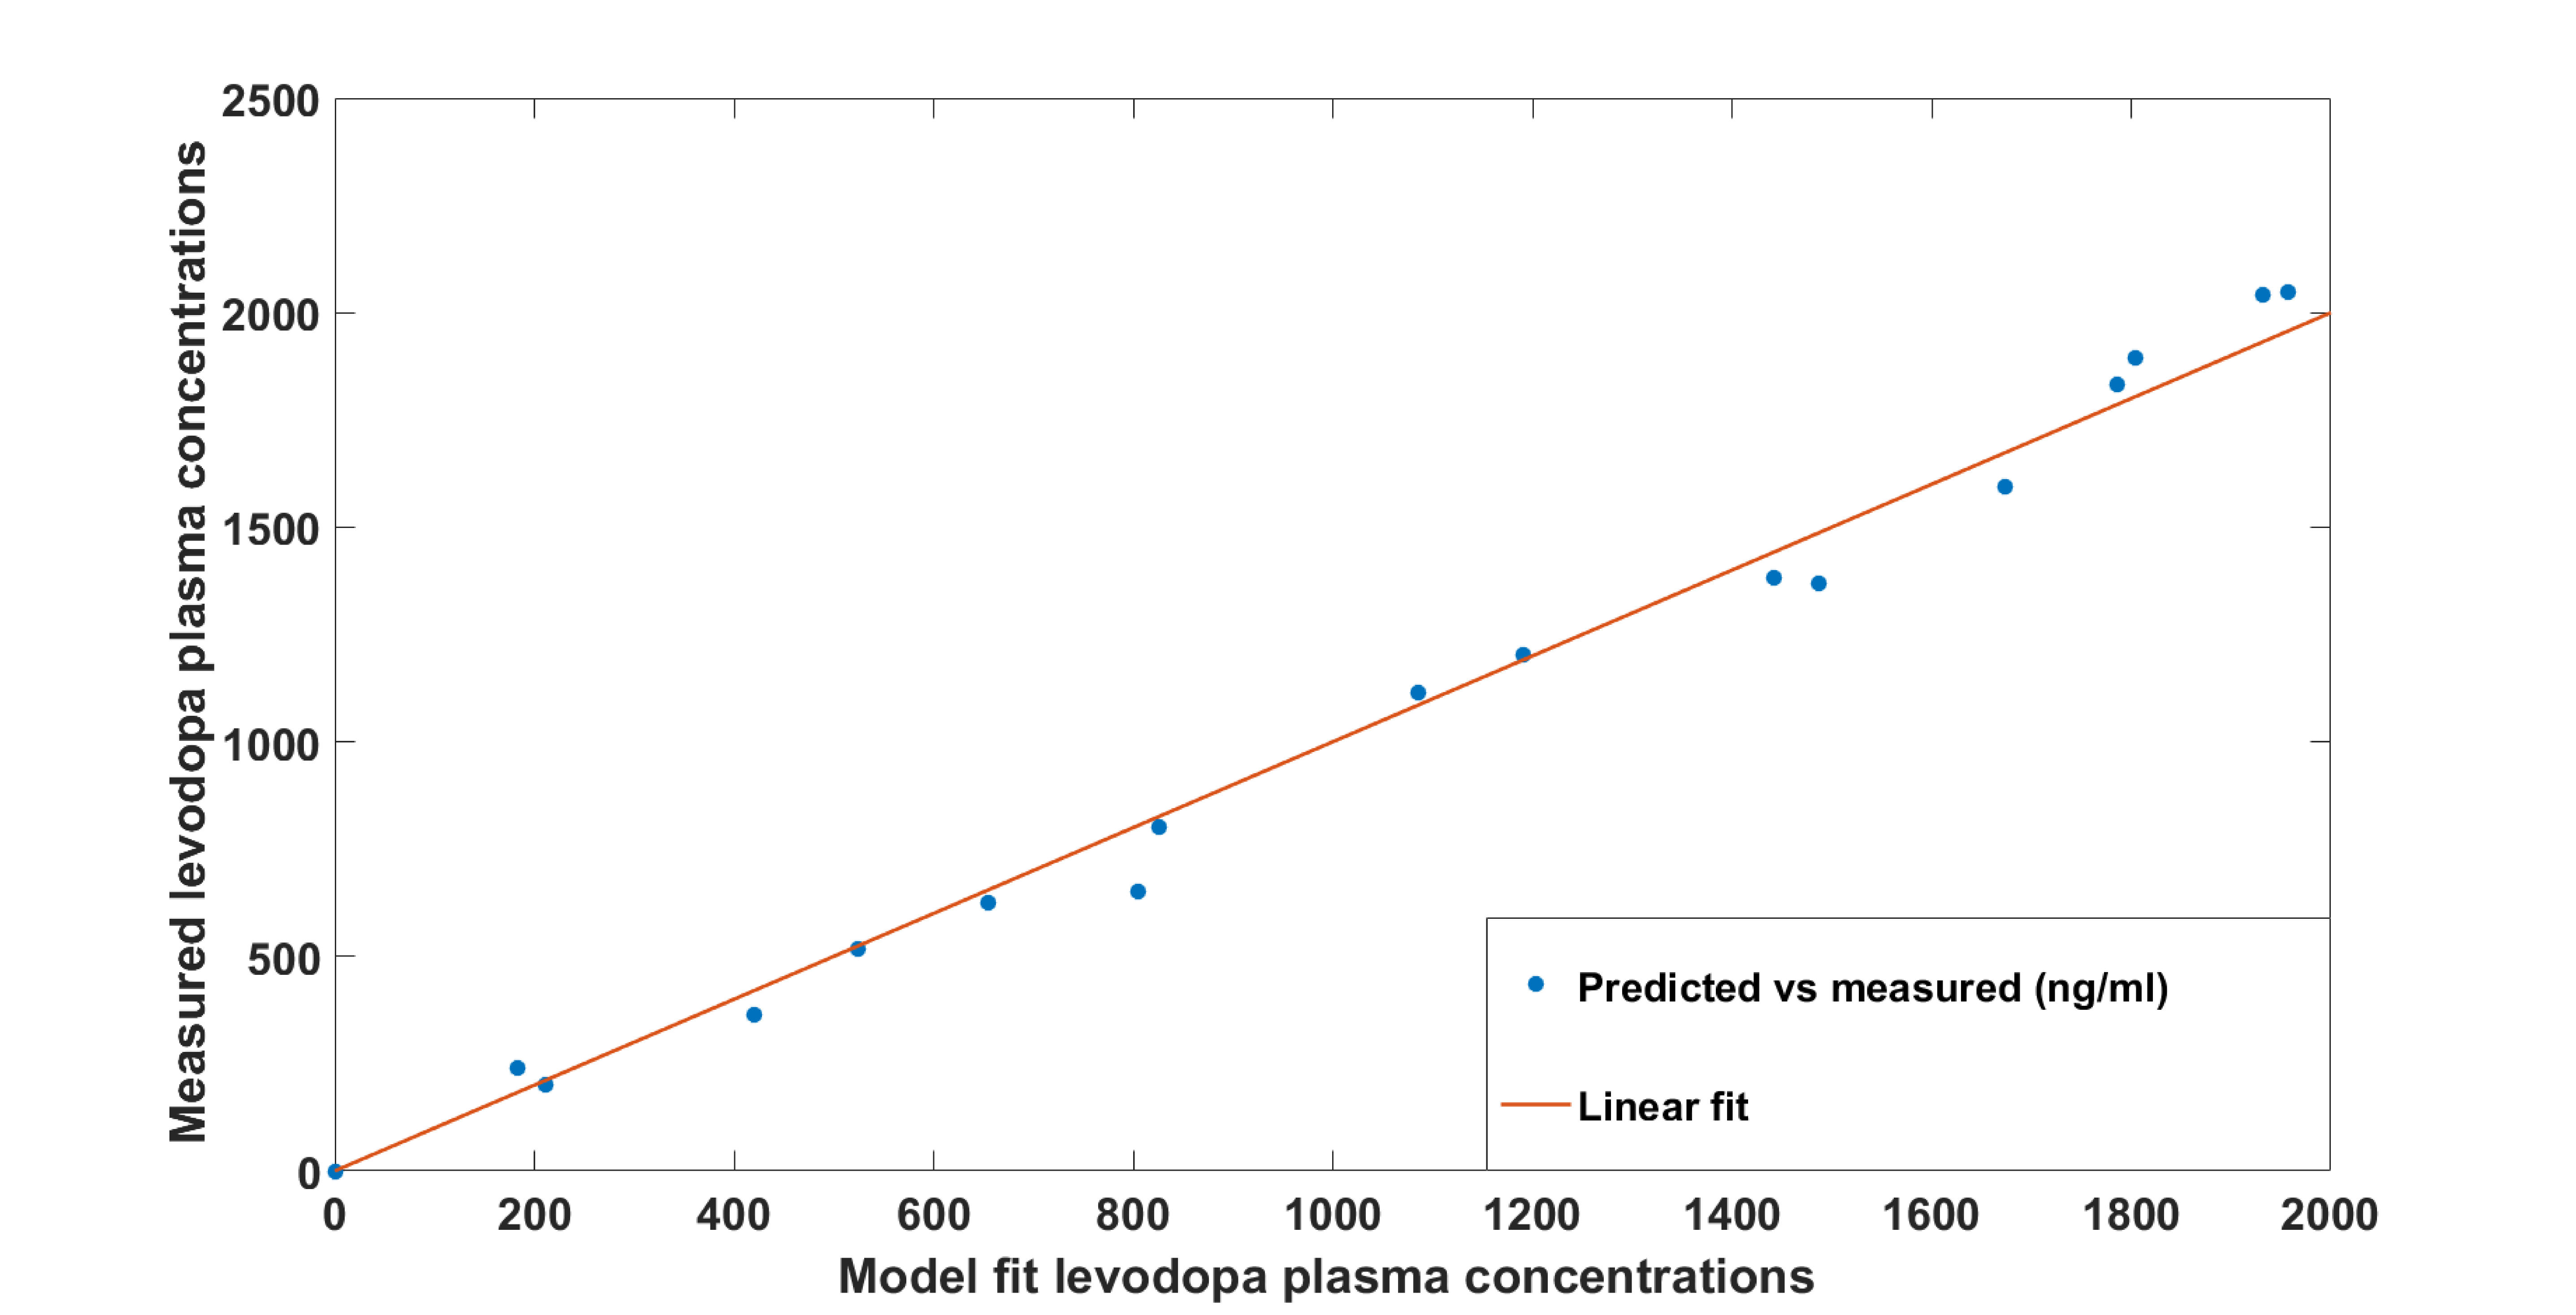
\includegraphics[width=\textwidth,height=\textheight,keepaspectratio]{levodopa/figS2.png}%Figure from images\Figure1.png
	\caption[Predicted versus measured levodopa kinetics.]{Goodness of fit plot of the simulated and measured levodopa plasma concentration in the fasted state, corresponding to figure S1-B. The model was simulated with the parameter values obtained from curve fitting the model on the observed data.}
	\label{fig:s2levo}
\end{figure}

\subsubsection{Sequential fit on two occasions: fasted and fed states} \label{levo:sp4}
First, the fitting of whole body generic PBPK model on fasted healthy volunteers plasma concentrations of levodopa, after 200 mg of standard formulation of levodopa, allowed to get the distribution and elimination parameters including the GER at the fasted state (3.96 h\textsuperscript{-1}). Then, all model parameters were fixed and only GER was estimated (0.33 h\textsuperscript{-1}) in the second occasion, i.e., the administration of levodopa with aproteic meal.
\begin{figure}[!htp]
\centering
	\includegraphics[width=\textwidth,height=\textheight,keepaspectratio]{levodopa/figS3.png}%Figure from images\Figure1.png
	\caption[Time course of levodopa fluxes.]{(Continued on the following page)}
	\label{fig:s3levo}
\end{figure}
\begin{figure}[t]
  \contcaption{Predicted flux values of the levodopa luminal antiporter (blue), cellular accumulation (turquoise), basolateral antiporter (green), and basolateral uniporter (yellow) in the seven small intestinal compartments, after \textit{Per os} administration of 200 mg of standard formulation of levodopa at the fasted state. For the intracellular accumulation (represented in the model with a reversible drain for levodopa (sink\_levodopa)), positive fluxes refer to accumulation, while negative fluxes represent secretion. The conversion to mmol/gDW\textsubscript{enterocyte}/hour was done as described in section adding levodopa reactions to sIEC.}% Continued caption
\end{figure}
\subsubsection{Amino acids ranking simulations} \label{levo:sp5}
\begin{figure}[!htp]
\centering
	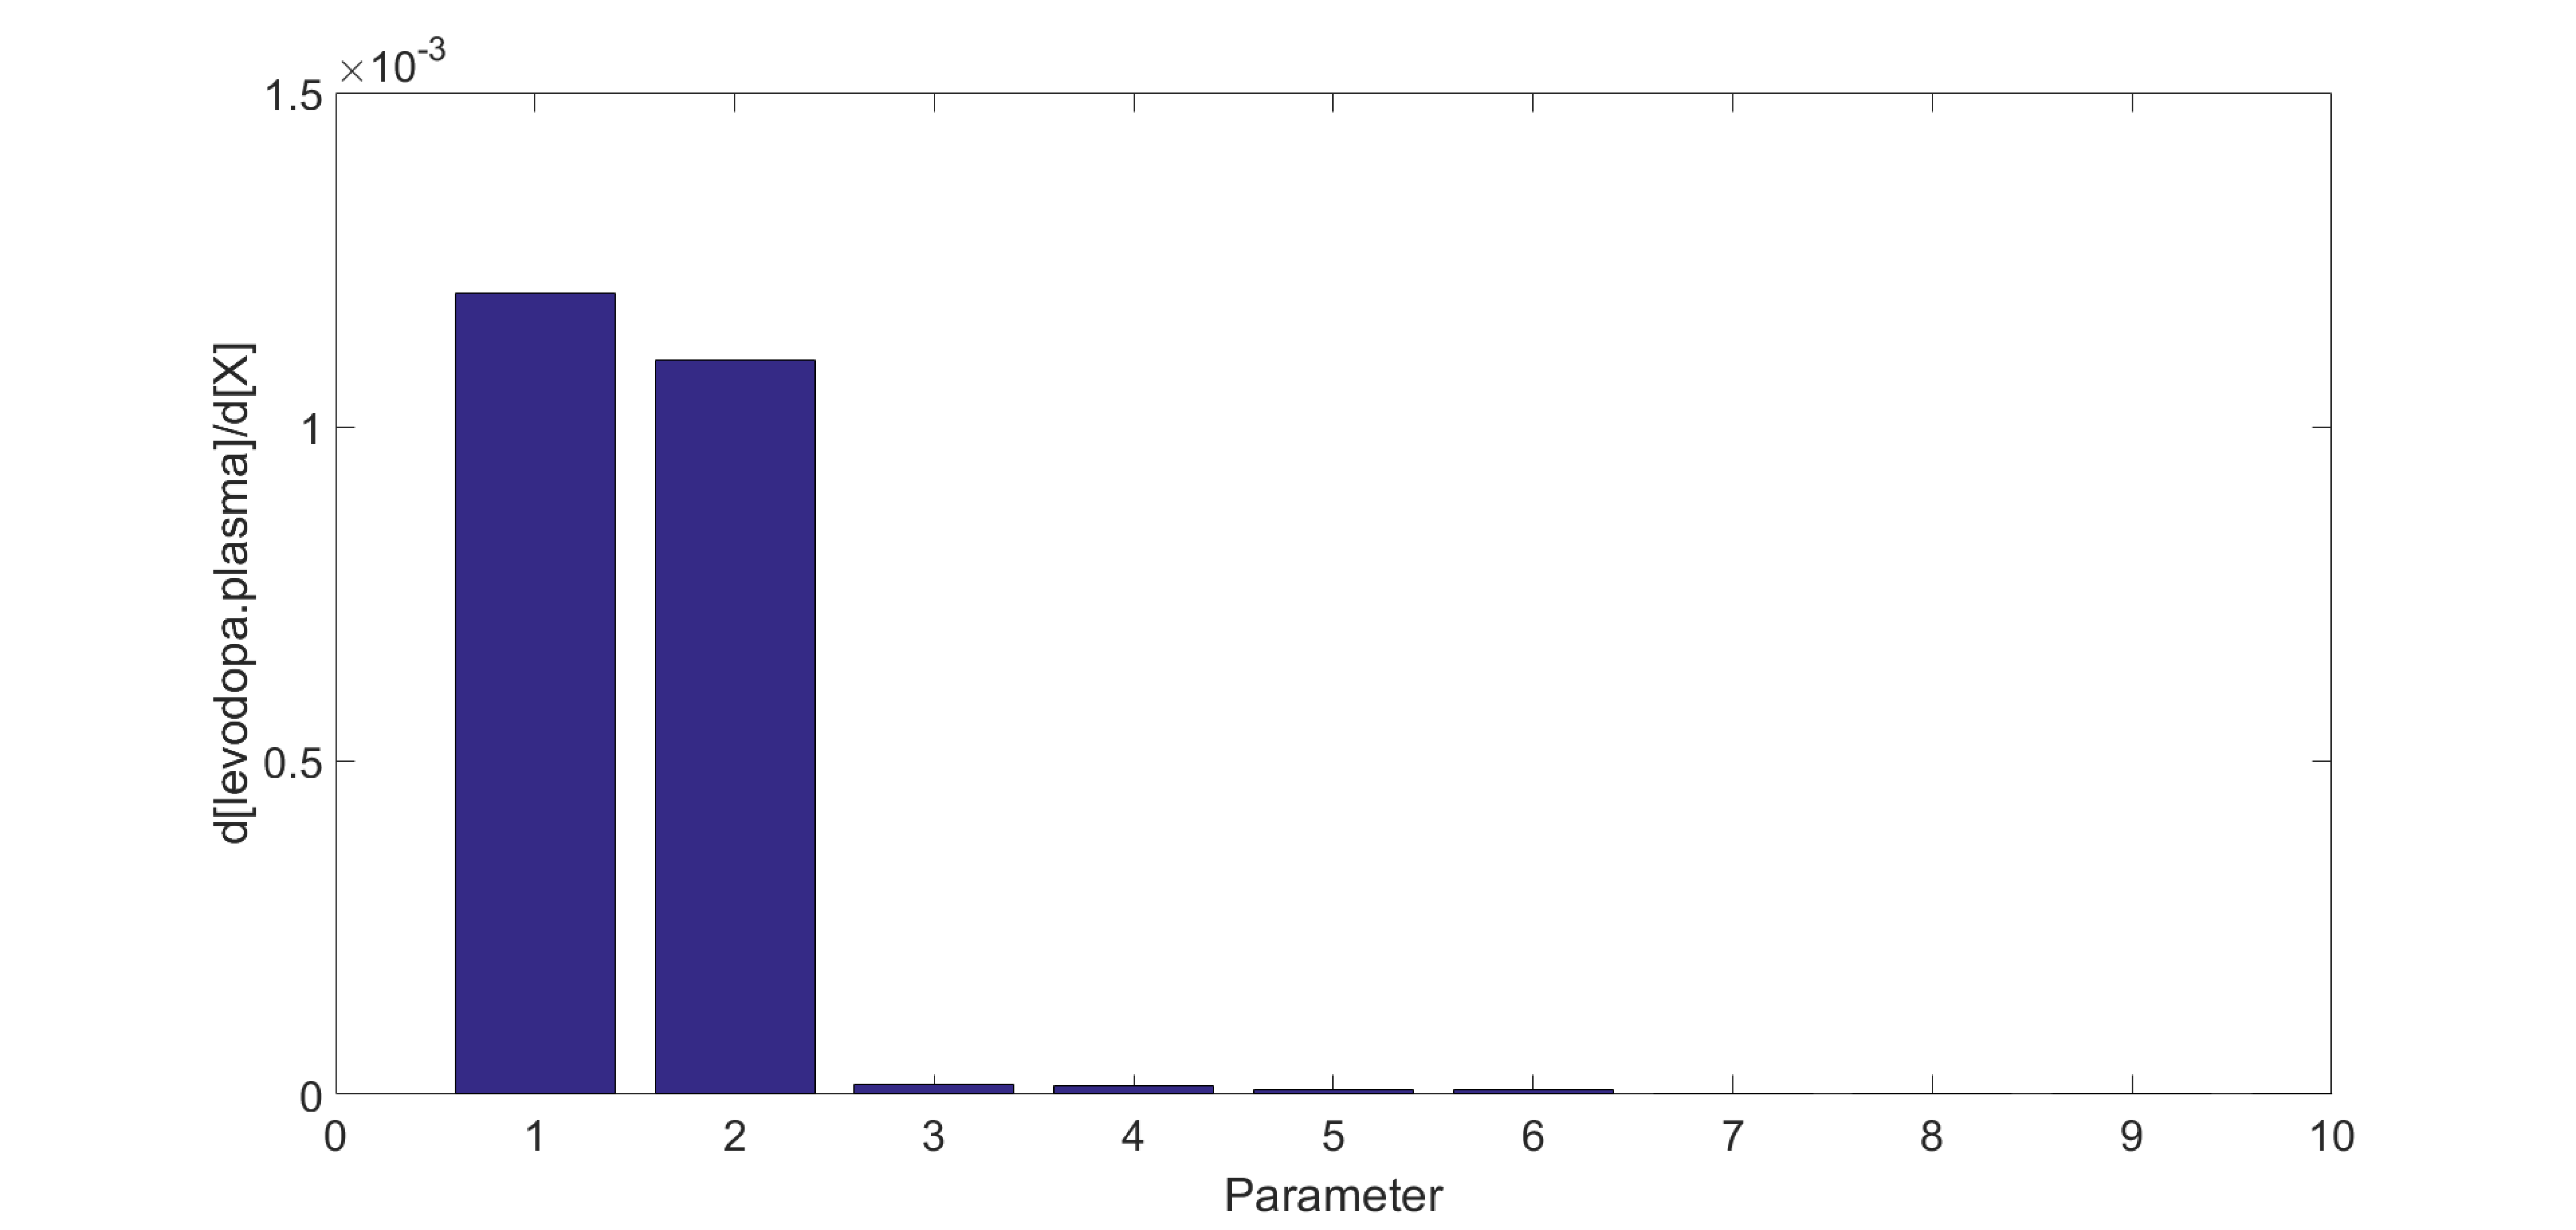
\includegraphics[width=\textwidth,height=\textheight,keepaspectratio]{levodopa/figS4.png}%Figure from images\Figure1.png
	\caption[Whole body PBPK model parameter sensitivity analysis.]{Whole body PBPK model parameter sensitivity analysis. Over 243 parameter, the 10 most influential absolute sensitivities are plotted. The first five parameters are described in Table \ref{tbl:tbls3}.}
	\label{fig:s4levo}
\end{figure}
The small intestine model was extended by adding a kidney compartment and brain compartment with the corresponding levodopa transport reactions (Figure S5). The objective function was set as the demand reaction for levodopa in the brain (Table \ref{tbl:tbls4}). The kidney and brain exchange reaction modeling took into account the affinity of substrates for the transporter, through assigning different arbitrary weights (Table \ref{tbl:tbls2}) for the fluxes representing each individual amino acid (Table \ref{tbl:tbls5}). The weighing coefficient is proportional to the amount of levodopa lost due to the competition with amino acids. The higher the competitive potential of the amino acid, the higher the assigned weight following the reported order of affinity of each transporter for amino acids \cite{verrey2000glycoprotein}. The coefficients were calibrated to take into account the tissue-specific competition potential of levodopa transporters in the following order: blood brain barrier, enterocyte, kidneys as supported by clinical investigation \cite{robertson1991influence,nutt1984off}. Trans-stimulation was not modeled in the kidneys and the brain as it is not supported by experimental evidence. The liver elimination was not formulated in the optimization problem as no records of competition were reported. 
An arbitrary intake of levodopa was set to 15 mg/l/h. Two thirds of this amount are absorbed by the small intestine. Since levodopa is antiported to the blood compartment, an excess of alanine, the contralateral substance to levodopa, was added. In order for levodopa to reach the blood brain barrier and the kidney, two demand reactions were added in these compartments. 30\% of levodopa was set to be eliminated by the kidneys and the rest transported through the blood brain barrier. Then a 3 mg/l/h of each amino acid was added simultaneously with levodopa and the fraction reaching the brain was calculated. Each amino acid either competed with levodopa in the small intestine, blood brain barrier or kidneys or all of the three organs. Basolateral trans-stimulation of levodopa intestinal secretion increases the absorption of levodopa. Since trans-stimulation was not proven in kidney and brain transporters, these were not modelled.  
\begin{figure}[!htp]
\centering
	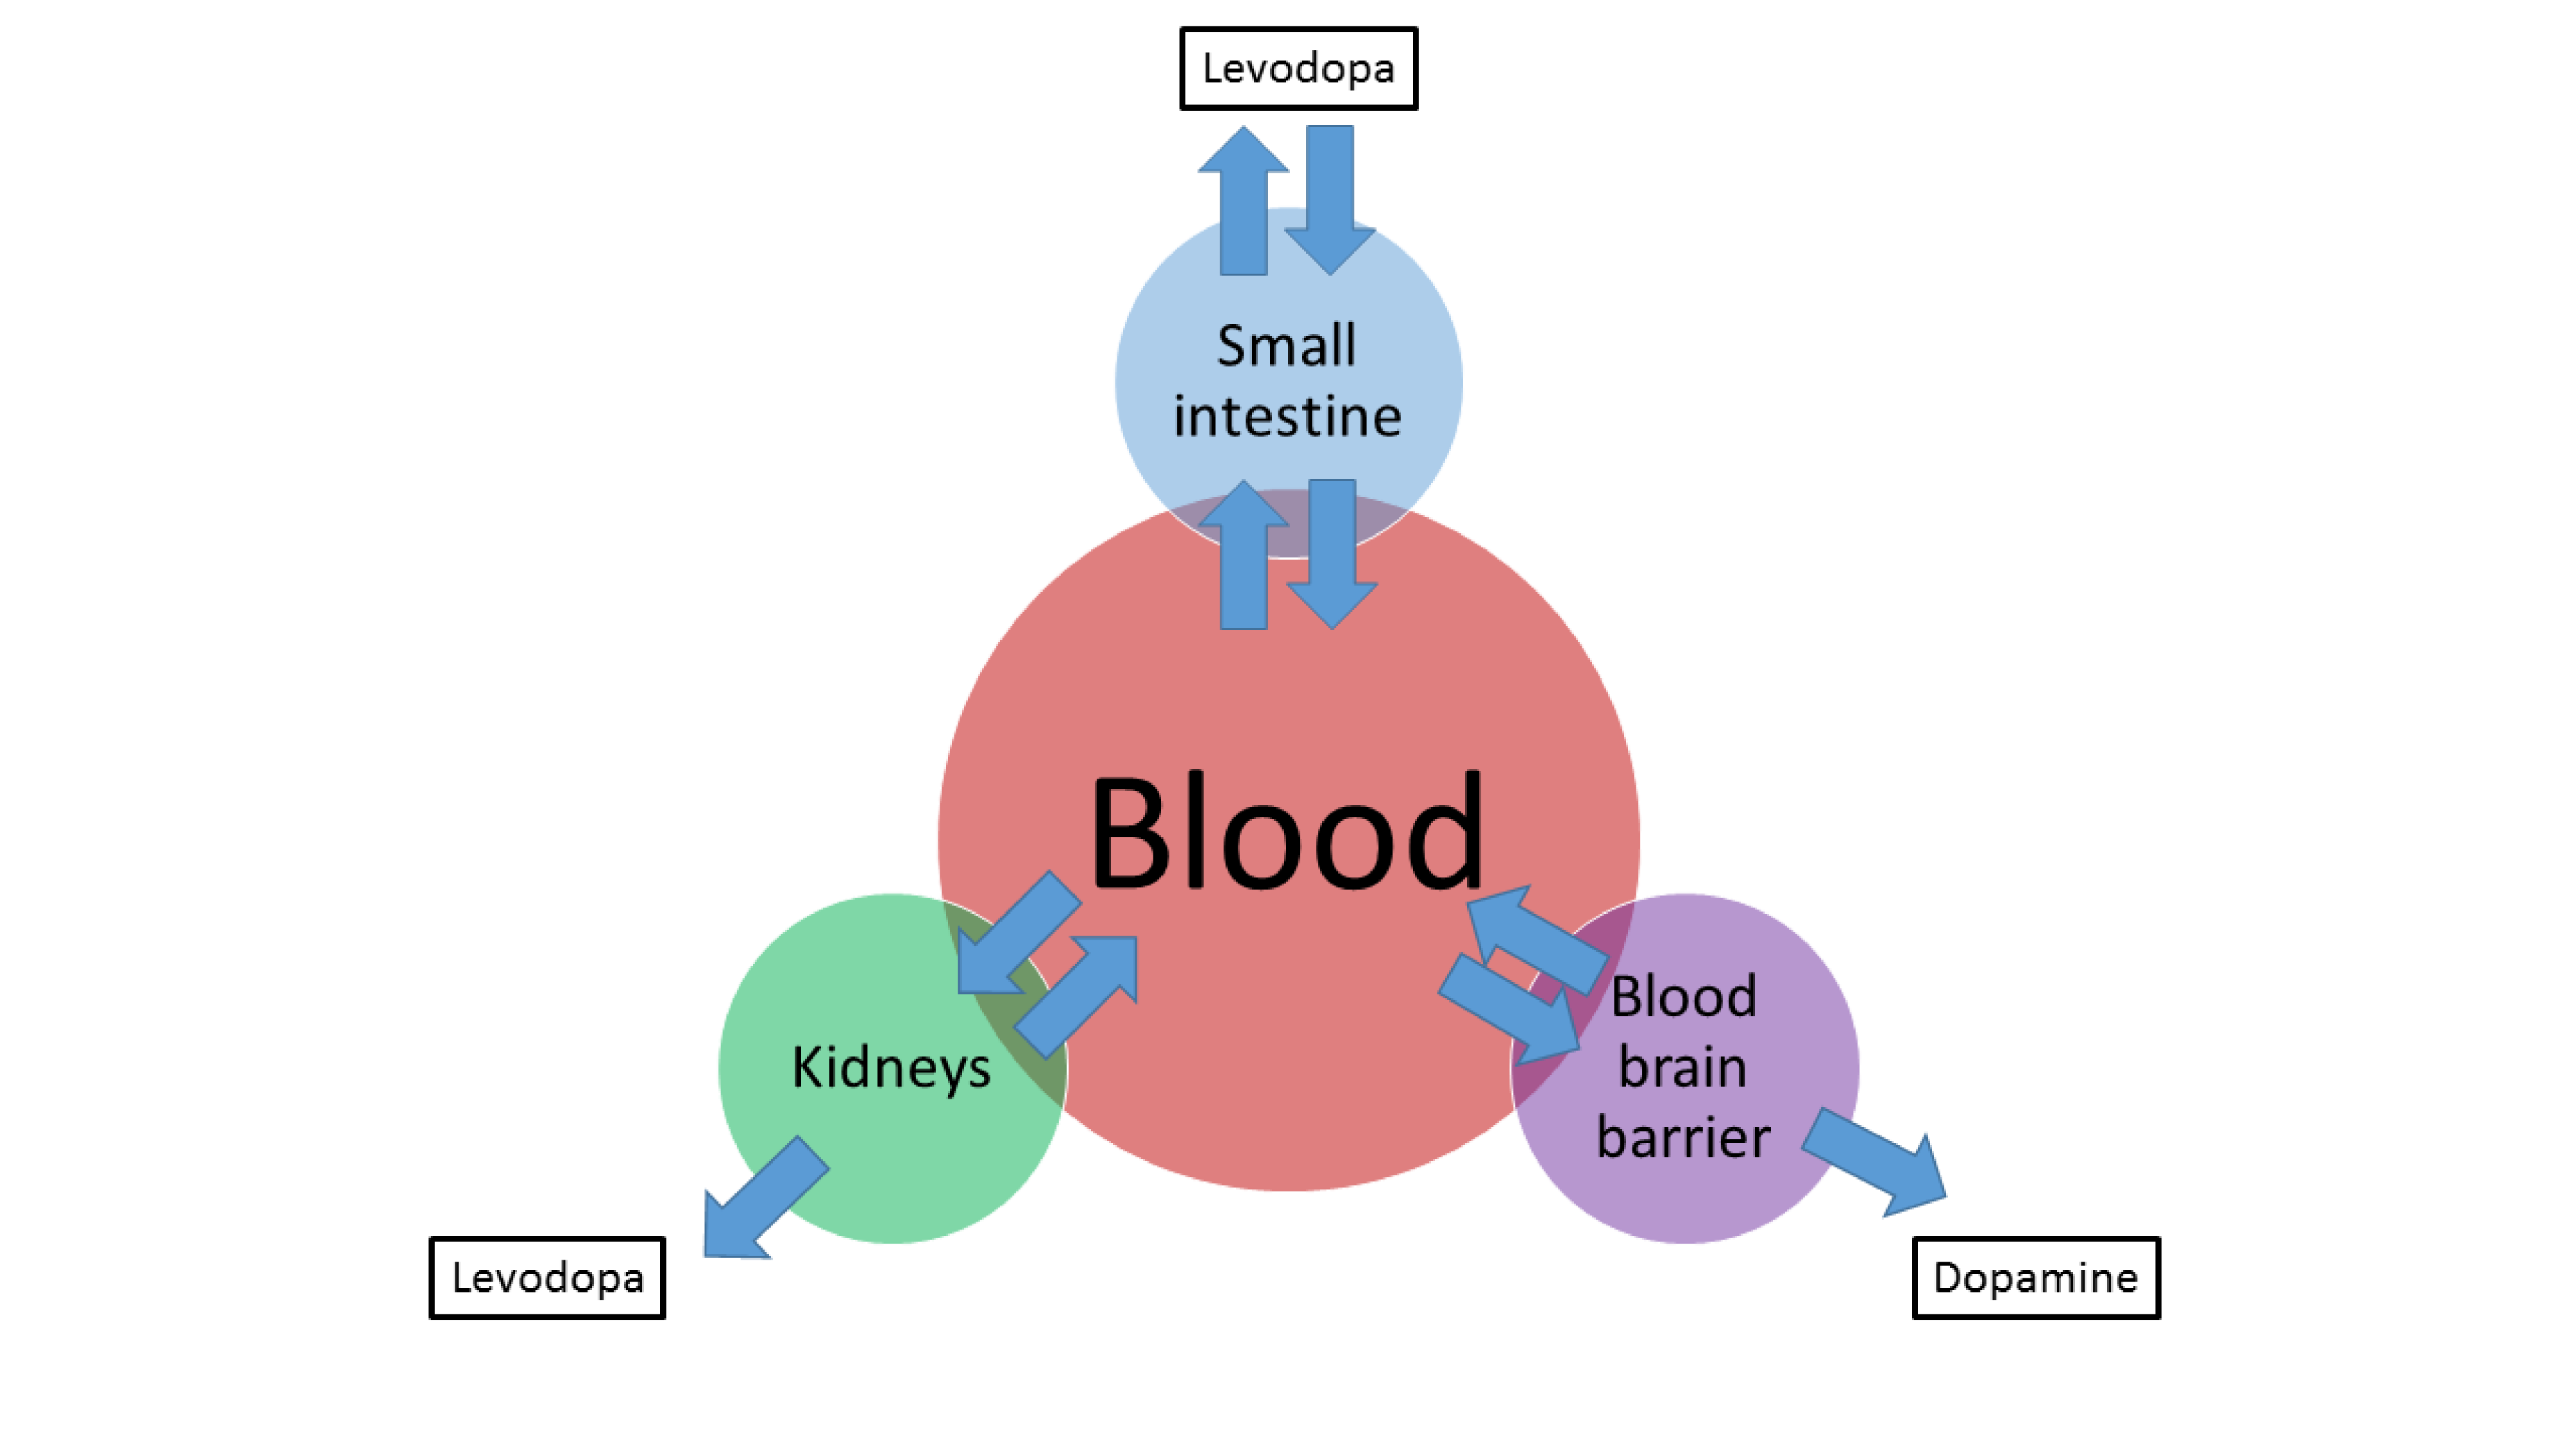
\includegraphics[width=\textwidth,height=\textheight,keepaspectratio]{levodopa/figS5.png}%Figure from images\Figure1.png
	\caption[Intestine, kidney, and brain simplified network of levodopa.]{Schematic view of small intestine, kidney and blood brain barrier transport reactions integration. The small intestine is represents through the genome-scale sIEC model, while only the transport reactions from blood to the organ were modelled in the other sites of competition (e.g., kidneys and brain compartments). }
	\label{fig:s5levo}
\end{figure}
%Path to supplementary material

\chapter{Supplementary material for Chapter 5}
\section{Supplementary tables}
\begin{table}[h]
\caption[Differentially expressed metabolic genes in type 1 diabetes.]{Differentially expressed metabolic genes in type 1 diabetes.}
\begin{center}
	\begin{tabular*}{\textwidth}{l @{\extracolsep{\fill}} ll}
	\hline
	Number & Gene symbol  & Gene expression variation        \\ 
	\hline
	1      & SV2A         & 0.33       \\
	2      & ADCY1        & 0.32        \\
	3      & AGT          & 0.65        \\
	4      & ELA2B        & 0.1        \\
    5      & PRPH2        & 2.04       \\
	6      & ALOX5        & 0.34        \\
	7      & G6PC2        & 0.03        \\
	8      & AMY1A        & 0.21        \\
	9      & ANPEP        & 2.67       \\
	10      & ITGAM       & 2.63        \\
	11      & PLA2G2A     & 4.85        \\
	12      & PFEB1       & 2.87        \\
	13      & ENO2        & 0.16       \\
	14      & ONECUT2     & 0.47        \\
	15      & PCIF1       & 3.86        \\
	16      & ACP5        & 2.69        \\
	17      & PECAM1      & 3.21       \\
	18      & TCIRG1      & 2.71        \\
	19      & FYN         & 3.16        \\
	20      & TLR1        & 2.6        \\
	21      & ABCC8       & 0.04       \\
	22      & TIMP3       & 2.9        \\
	23      & PCDHA12     & 0.2        \\
	24      & CD36        & 4.06        \\
	\hline
	\end{tabular*}
\end{center}
\label{GIM:tbls1}%descriptive label to refer to figure in text
\end{table}

\clearpage

\begin{table}[h]
\caption[Pancreatic reactions corresponding to the differentially expressed genes in type 1 diabetes.]{Pancreatic reactions corresponding to the differentially expressed genes in type 1 diabetes where P refers to pancreas, lu to lumen, and bp to portal blood.}
\begin{center}
	\begin{tabular*}{\textwidth}{l @{\extracolsep{\fill}} ll}
	\hline
	Reaction name      & Reaction name  & Reaction name\\ 
	\hline
Pancreas\_ALACYSNaEx  & Pancreas\_SERALANaEx & Pancreas\_SIAASEly \\    	
Pancreas\_ALADGLNexR  & Pancreas\_SERCYSNaEx & Pancreas\_r0636 \\  	
Pancreas\_ALADGLYexR  & Pancreas\_SERDGLNexR & Pancreas\_BGAL1l \\   	
Pancreas\_ALAGLNexR   & Pancreas\_SERDGLYexR & Pancreas\_NEU11l \\   	
Pancreas\_ALAGLYexR   & Pancreas\_SERGLNexR  & Pancreas\_CRNATBtc[bpP] \\   	
Pancreas\_ALASERNaEx  & Pancreas\_SERGLYexR  & Pancreas\_ALACYSNaEx \\   	
Pancreas\_ALAt4       & Pancreas\_SERt4      & Pancreas\_ALADGLNexR \\   	
Pancreas\_ALATHRNaEx  & Pancreas\_SERTHRNaEx & Pancreas\_ALADGLYexR \\  	
Pancreas\_ASNt4       & Pancreas\_THRALANaEx & Pancreas\_ALAGLNexR\\   	
Pancreas\_ATPS4m      & Pancreas\_THRCYSNaEx & Pancreas\_ALAGLYexR \\   	
Pancreas\_CATm        & Pancreas\_THRGLNexR  \\   	
Pancreas\_CATp        & Pancreas\_THRGLYexR \\   	
Pancreas\_CSNAT2x     & Pancreas\_THRSERNaEx \\   	
Pancreas\_CYSALANaEx  & Pancreas\_THRt4 \\   	
Pancreas\_CYSGLUexR   & Pancreas\_TRPt4 \\   	
Pancreas\_CYSGLYexR   & Pancreas\_TYRt4 \\   	
Pancreas\_CYSSERNaEx  & Pancreas\_VALt4 \\   	
Pancreas\_CYSt4       & Pancreas\_r0637 \\   	
Pancreas\_CYSTHRNaEx  & Pancreas\_r0997 \\   	
Pancreas\_DGNSKm      & Pancreas\_SUCCCROT \\   	
Pancreas\_FMNAT       & Pancreas\_34DHPHELAT1tc \\   	
Pancreas\_FRUt1r      & Pancreas\_4OHPROIMINOtc \\   	
Pancreas\_FTHFDH      & Pancreas\_HISyLATthc \\   	
Pancreas\_FTHFL       & Pancreas\_LEUPHELAT2tc  \\   	
Pancreas\_GALASE19ly  & Pancreas\_3HCO3\_NAt \\   	
Pancreas\_GLCt1r      & Pancreas\_4HPROLTASCT1  \\   	
Pancreas\_GLNS        & Pancreas\_ASPPROASCT1\\   	
Pancreas\_GLNt4       & Pancreas\_GLUPROASCT1 \\   	
Pancreas\_GLYt4       & Pancreas\_IPDDI \\   	
Pancreas\_HOXG        & Pancreas\_25HVITD3tin \\   	
Pancreas\_ILEt4       & Pancreas\_LCAT25e \\   	
Pancreas\_IPDDIx      & Pancreas\_GLCRt1 \\   	
Pancreas\_LACZe       & Pancreas\_SELMETHte \\   	
Pancreas\_LEUt4       & Pancreas\_BGAL2l \\   	
Pancreas\_METt4       & Pancreas\_3HCO3\_NAt[luP] \\   	
Pancreas\_MTHFDm      & Pancreas\_FRUt1r[luP] \\   	
Pancreas\_PHEt4       & Pancreas\_GLCRt1[luP] \\   	
Pancreas\_PPAer       & Pancreas\_GLCt1r[luP] \\   	
Pancreas\_PROt4       & Pancreas\_GLUPROASCT1[luP] \\   	
Pancreas\_S6TASE8ly   & Pancreas\_ARGLYSex \\   	
Pancreas\_S6TASE9ly   & Pancreas\_GALASE1ly \\   	

	\hline
	\end{tabular*}
\end{center}
\label{GIM:tbls2}%descriptive label to refer to figure in text
\end{table}

\clearpage

\begin{table}[h]
\caption[Parameters of the dynamical model simulations.]{Parameters of the dynamical model simulations.}
\begin{center}
	\begin{tabular*}{\textwidth}{l @{\extracolsep{\fill}} ll}
	\hline
	Setting & Dose administered (kg)  & Administration time (mn)        \\ 
	\hline
	Intravenous Glucose Tolerance Test       & 0.04         & 15       \\
	(IVGTT) & & \\
	Intravenous Insulin Tolerance Test      & $1.02*10^{-7}$        & 15        \\
	(IVITT)& & \\
	Baseline Glucose      & 0          & 0        \\
	Subcutaneous Insulin Bolus     & $1.02*10^{-7}$        & 15        \\
	(SCIB) & & \\
    Subcutaneous Insulin Infusion       & $3.66*10^{-7}$        & 600       \\
    (SCII) & & \\
	Oral liquid glucose solution      & 0.1        & 0        \\
	(WB-Liquid) & & \\
	Solid Meal      & 0.04        & 0        \\
	(WB-Solid) & & \\
	\hline
	\end{tabular*}
\end{center}
\label{GIM:tbls3}%descriptive label to refer to figure in text
\end{table}

\clearpage

\begin{table}[h]
\caption[Selected functions linked to type 1 diabetes symptomatology.]{Selected functions linked to type 1 diabetes symptomatology.}
\begin{center}
	\begin{tabular*}{\textwidth}{l @{\extracolsep{\fill}} lll}
	\hline
	Enriched reaction & Metabolites involved  & Type 1 diabetes related & Related        \\ 
	& & process & symptoms \\
	\hline
	Muscle\_ADCim            & Acetoacetate          & Ketone bodies disrupted  & Ketoacidosis\\
	Brain\_FUMAC             & & metabolism & \\
	Liver\_r2079             &         &     &    \\
	Colon\_r2082             & & & \\\cmidrule{1-4}
	Liver\_biomass\_reaction & Glycogen, ATP, & Glycogen liver     & Hepatomegaly in   \\
	Liver\_SPHS1Pt2e         & ADP       &    deposition   & uncontrolled \\
	Liver\_FPGS4             & & & diabetes\\
    Liver\_CERK              &        &     &   \\
    Liver\_DPCOAK            & & & \\
	Liver\_FTHFL             &         &   &      \\
	Liver\_GLYK 			 & & & \\
	Liver\_KHK               &        &        & \\\cmidrule{1-4}
	Retina\_O2Stm            & Superoxide & Free radicals production & Retinopathy \\
	Retina\_SPODM            & & & \\\cmidrule{1-4}
	Heart\_RE3273C           & Phosphoinositides & Regulation of & Cardiovascular \\
	Heart\_PIACGT 			 & & cardiomyocyte & disease\\
	Heart\_CDIPTr 			 & & metabolism & \\
	\hline
	\end{tabular*}
\end{center}
\label{GIM:tbls4}%descriptive label to refer to figure in text
\end{table}

\clearpage
\begin{table}[h]
\caption[Enriched KEGG terms in type 1 diabetes.]{Enriched KEGG terms in the genes coding for the upregulated metabolic fluxes in type 1 diabetes.}
\begin{center}
	\begin{tabular*}{\textwidth}{l @{\extracolsep{\fill}} lll}
	\hline
	Enriched pathway & p-value  & Adjusted p-value & Z-score        \\ 
	\hline
	Metabolic pathways           & 4.463e-216& 8.123e-214    & -2.01 \\
	Oxidative phosphorylation    & 9.328e-59 & 8.489e-57 & -1.80\\
	Parkinson's disease          & 1.931e-38 & 1.171e-36   &   -1.72 \\
	Carbon metabolism            & 5.054e-37 & 2.300e-35 & -1.63 \\
	Glycolysis / Gluconeogenesis & 4.251e-31 & 1.548e-29      & -1.88     \\
	Alzheimer's disease          & 7.035e-31 & 2.134e-29       & -1.72 \\
	Huntington's disease         & 1.856e-27 & 4.827e-26 & -1.75\\
    Non-alcoholic fatty liver disease (NAFLD) & 1.514e-23       & 3.061e-22    & -1.76  \\
    Biosynthesis of amino acids            & 9.612e-24 & 2.187e-22 & -1.55\\
	Fatty acid degradation                 & 1.740e-19        & 3.167e-18  &  -1.44    \\
	\hline
	\end{tabular*}
\end{center}
\label{GIM:tbls5}%descriptive label to refer to figure in text
\end{table}

\clearpage

\begin{table}[h]
\caption[Small molecules that reverse type 1 diabetes metabolic fluxes.]{Small molecules that reverse the metabolic flux distribution associated to type 1 diabetes.}
\begin{center}
	\begin{tabular*}{\textwidth}{l @{\extracolsep{\fill}} ll}
	\hline
	Rank & Small molecule  & Class / Nomenclature         \\ 
	\hline
	1    & Terfenadine & Antihistaminic (withdrawn)   \\
	2    & SB 216641 hydrochloride & 5 HT1-B antagonist (anxiolytic effects) \\
	3    & Mibefradil dihydrochloride & Calcium channel blocker   \\
	4    & Maprotiline hydrochloride & Tetracycline antidepressant \\
	5    & L-733,060 hydrochloride & Antidepressant/anxiolytic         \\
	6    & AY 9944  & Specific inhibitor of cholesterol biosynthesis        \\
	7    & Amlodipine besylate & Calcium channel blocker \\
    8    & Wiskostatin        & (Neuronal-WASP inhibitor)     \\
    9    & Thioridazine & Antipsychotic \\
	\hline
	\end{tabular*}
\end{center}
\label{GIM:tbls6}%descriptive label to refer to figure in text
\end{table}


\clearpage
\section{Supplementary figures}
\subsection{Construction of the hybrid model} \label{GIM:sp1}
We combined the glucose-insulin ODE-based dynamical model (GIM) \cite{schaller2013generic} with the organ-resolved constraint-based model (Harvey) \cite{thiele2018metabolism} into a multi-scale model (dHarvey).\\
GIM was originally coded in the PKSIM-MOBI \cite{eissing2011computational} format and was subsequently converted using PKSIM into a set of ODEs in MATLAB (2014b, Natick, MA, USA) and solved using \textit{ode15s}. The model described the complex glucose regulatory mechanism by insulin and glucagon in all organs using a whole-body PBPK model. In the intestinal tract, it models the intestinal regulation of glucose by incretin hormones (glucagon-like peptide 1 (GLP1) and gastric inhibitory polypeptide (GIP)) and the absorption by glucose carriers such as SGLT1 and SGLT2. In each organ and particularly the target organs i.e., liver, pancreas, brain, fat, and muscle, GIM represented a number of processes related to insulin action such as its diffusion from the blood to the extracellular space, the metabolism of glucose by red blood cells, the internalization of insulin by endothelial cells, the clearance by the lymphatic circulation, the binding and internalisation of insulin receptors followed by the release of glucose receptors, and the storage of glycogen. Since insulin acts with a relatively low dose, its binding to the receptor can modulate its pharmacokinetics. Consequently, GIM modelled the target-mediated drug disposition (TMDD) of insulin in relation to its pharmacodynamics. The organs modelled were the bones, brain, fat, gallbladder, gonads, heart, kidney, large and small intestine, liver, lung, muscle, pancreas, skin, spleen, and stomach connected by extracellular compartments and biofluids such as arterial and venous blood, portal vein, intestinal lumen, and saliva. Each organ is further compartmentalized into anatomical and histological units such as the intracellular space, the interstitial space, and the endothelial compartment. The model parameters were validated using several datasets of glucose tolerance tests and closed-loop insulin administration in patients \cite{regittnig1999plasma,sorensen1985physiologic,el2010bihormonal}. The model was applied in a number of applications mainly pertaining to closed-loop inuslin administration in T1D patients \cite{wadehn2016multiscale,schaller2012new,schaller2016robust}, and the estimation of cell proliferation rate in human using labelled glucose \cite{lahoz2017physiologically}.\\
Harvey is the organ-resolved constraint-based metabolic model of the human body \cite{thiele2018metabolism}. It represents the metabolic network of 20 organs, six sex organs, and six blood cells totalling more than 80,000 reaction, 50,000 metabolite, and 100 subsystem. The model was based on the global reconstruction of human metabolism (Recon) through the context-specific modeling of organs using human proteomic data and the manual curation of organ-specific pathways. The organs were connected through biofluids and exchange compartments taking into account inter-organ cycles and crosstalk. The model takes into account physiological constraints such as the heart rate, basal metabolic rate, renal filtration, and oxygen uptake.\\
Coupling GIM with Harvey fell under one of the following situations (Figure \ref{fig:GIM0}):\\
\begin{enumerate}
\item When the fluxes in GIM and Harvey corresponds exactly, the flux in the metabolic model was set to the one in the dynamical model,
\item When metabolites are identical in both models, the corresponding b vector entry in the metabolic model is set equal to the rate-of-change of metabolite concentration,
\item When to a specific reaction in the dynamical model, correspond several reactions in the metabolic model, the reactions are pooled in Harvey such as their total fluxes equals the reaction flux in the dynamical model,
\item Finally, when to specific metabolite in the dynamical model, correspond several metabolites, they are pooled into one super metabolite through merging the corresponding rows in the stoichiometric matrix. In the dynamical model, the blood cells are pooled in one compartment, wherein in the metabolic model, each blood cell is represented apart.
\end{enumerate}
\begin{figure}[!htp]
\centering
	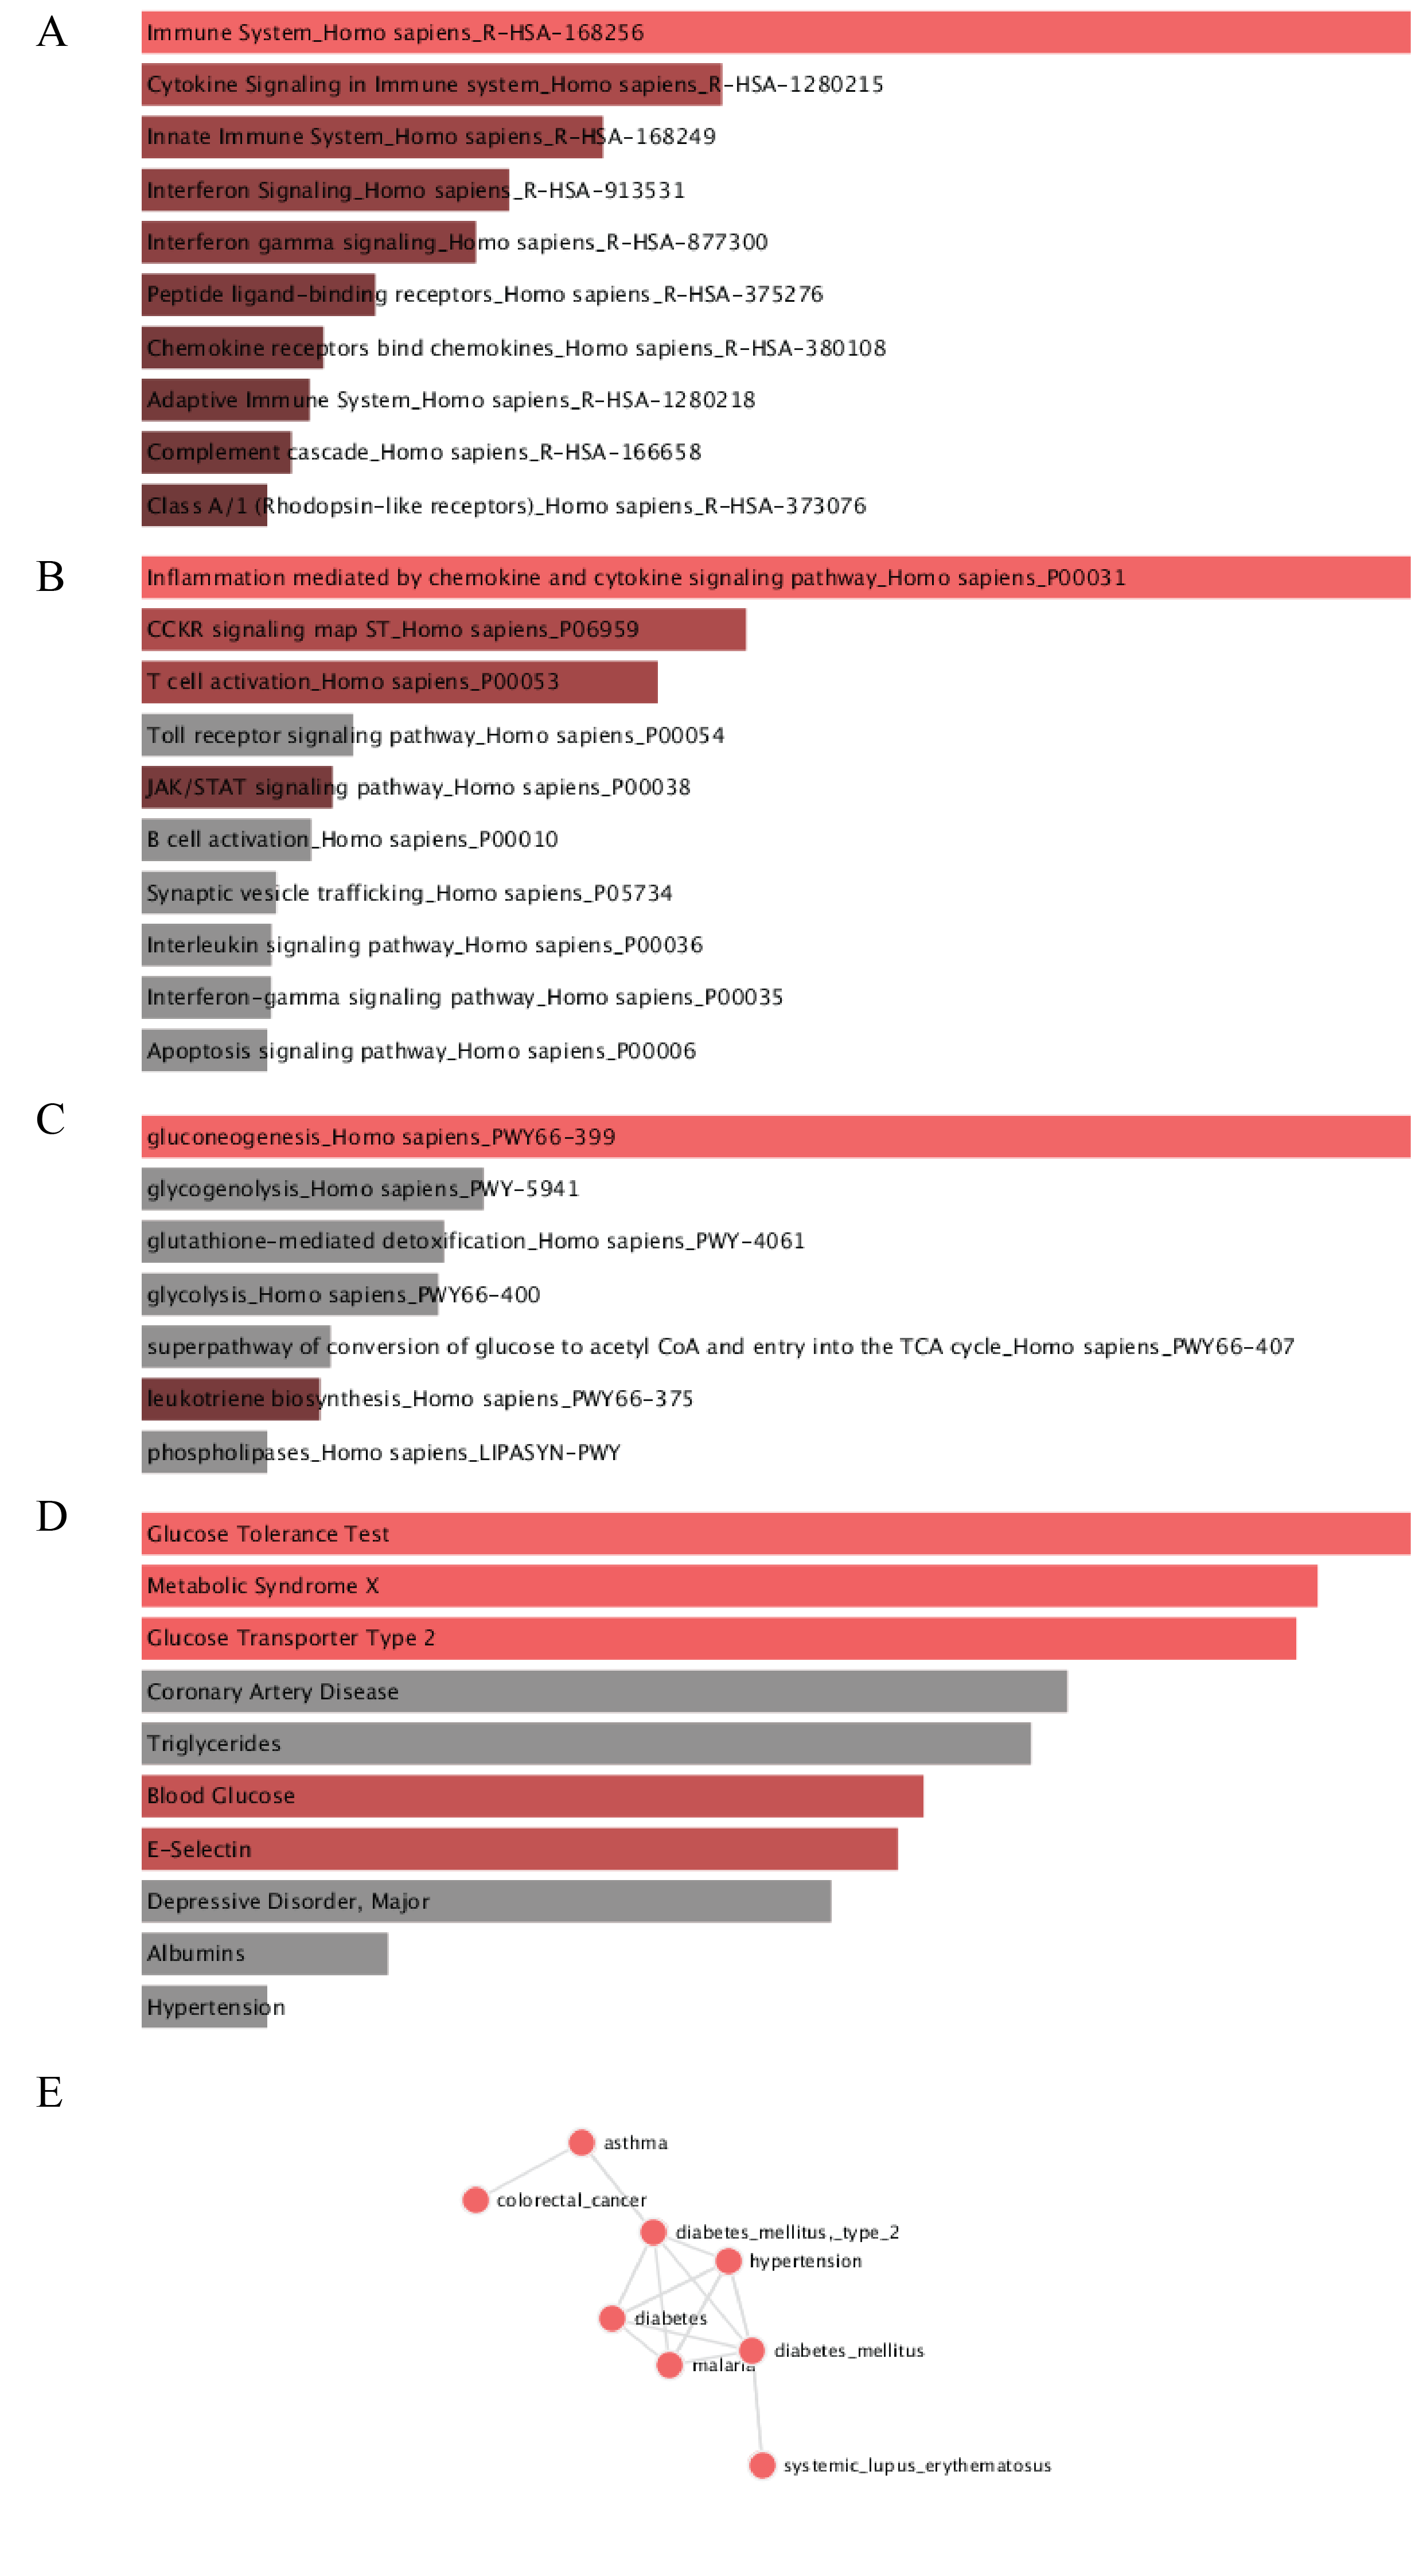
\includegraphics[width=\textwidth,height=\textheight,keepaspectratio]{GIM/figureS1.png}%Figure from images\Figure1.png
	\caption[Enrichment analysis of the type 1 diabetes genes.]{(Continued on the following page)}
	\label{fig:s0GIM}
\end{figure}
\begin{figure}[t]
  \contcaption{Enrichment analysis of the type 1 diabetes differentially expressed genes in A- Reactome and B-Panther database and the enrichment of the metabolic genes in C- the HumanCyc database, D- the dbGap database, and the E- OMIM database.}% Continued caption
\end{figure}
\subsection{Simulation setting} \label{GIM:spsim}
\subsubsection{Tolerance tests}
We used dHarvey to simulate the outcome of the different tolerance tests.
The kinetic parameters provided with the GIM model were used to represent the doses and time of intake. We applied the constraints dynamically on Harvey in each time step following the indirect coupling method. In IVGTT, where a dose of glucose is injected intravenously, we added an exchange reaction to represent the intake of glucose in the blood \textit{glc\_D[bc]} during the 15 mn of infusion (67.7 mmol/5mn). Consequently, we solved Harvey using pFBA \cite{lewis2010omic} assuming a whole-body maintenance objective function and aggregated the results in a matrix for each time step comprised of the tolerance tests in columns and the metabolic fluxes in rows. We reduced the matrix through PCA, and plotted the time-course of the first component (Figure \ref{fig:GIM1}-E) to illustrate the whole-body metabolic shift induced by a insulin and glucose tolerance tests. The points were fit on a 6\textsuperscript{th} order polynomial curve (Figure \ref{fig:GIM1}-E).\\
Furthermore, in order to assess if the dHarvey model was sensitive to the dynamical constraints applied from the GIM model, we aggregated the pFBA simulation results over 600 mn of simulation per 5mn time step. In each tolerance test simulation, we built a feature matrix comprised of the whole-body metabolic fluxes  in columns and the tolerance test in each time step in rows. With a time step of 5mn, 120 simulation result in T1D and healthy formed the 240 rows. We then reduced each matrix of the tolerance test using PCA. We took the 10 first component of the PCA, as they were significant at $p<0.001$. The component significance was assessed through 100 random permutation of the columns followed by PCA on the perturbed matrix. The 10 first component were then used as features in a binary SVM to classify healthy and T1D based on whole-body fluxes in each tolerance test. We used an SVM with a Gaussian kernel and performed 3-fold cross-validation on the training set (80\%) and predicted the labels of the test set (20\%). The data was standardized and the process was repeated 100 times taking every time a different partition of the training and test set.
We choose to use significant components as features instead of performing feature selection on the whole-body fluxes as the focus was the assessment of dHarvey sensitivity towards glucose and insulin challenges and the subsequent whole-body metabolic shift. The fluxes used in each time step are one among many possible solutions in the AOS space, and cannot be used as conclusive evidence on the disrupted metabolic pathways in T1D and healthy, even though pFBA reduces considerably the AOS space \cite{toroghi2016multi}. We addressed the question of disrupted  metabolic pathways in T1D through performing FVA in T1D and healthy models and using all the solution vectors of the AOS as a kernel for comparison. dHarvey was predictive towards T1D and healthy states in the tolerance tests (Figure (Figure \ref{fig:GIM1}-E), moreover when we used insulin and glucose challenges as classes in the SVM instead of T1D and healthy, whole-body fluxes were predictive towards them as well (Figure \ref{fig:s1GIM}). Taken together, dHarvey is predictive towards both the condition (T1D and healthy) and the perturbation (insulin and glucose challenges).
\begin{figure}[!htp]
\centering
	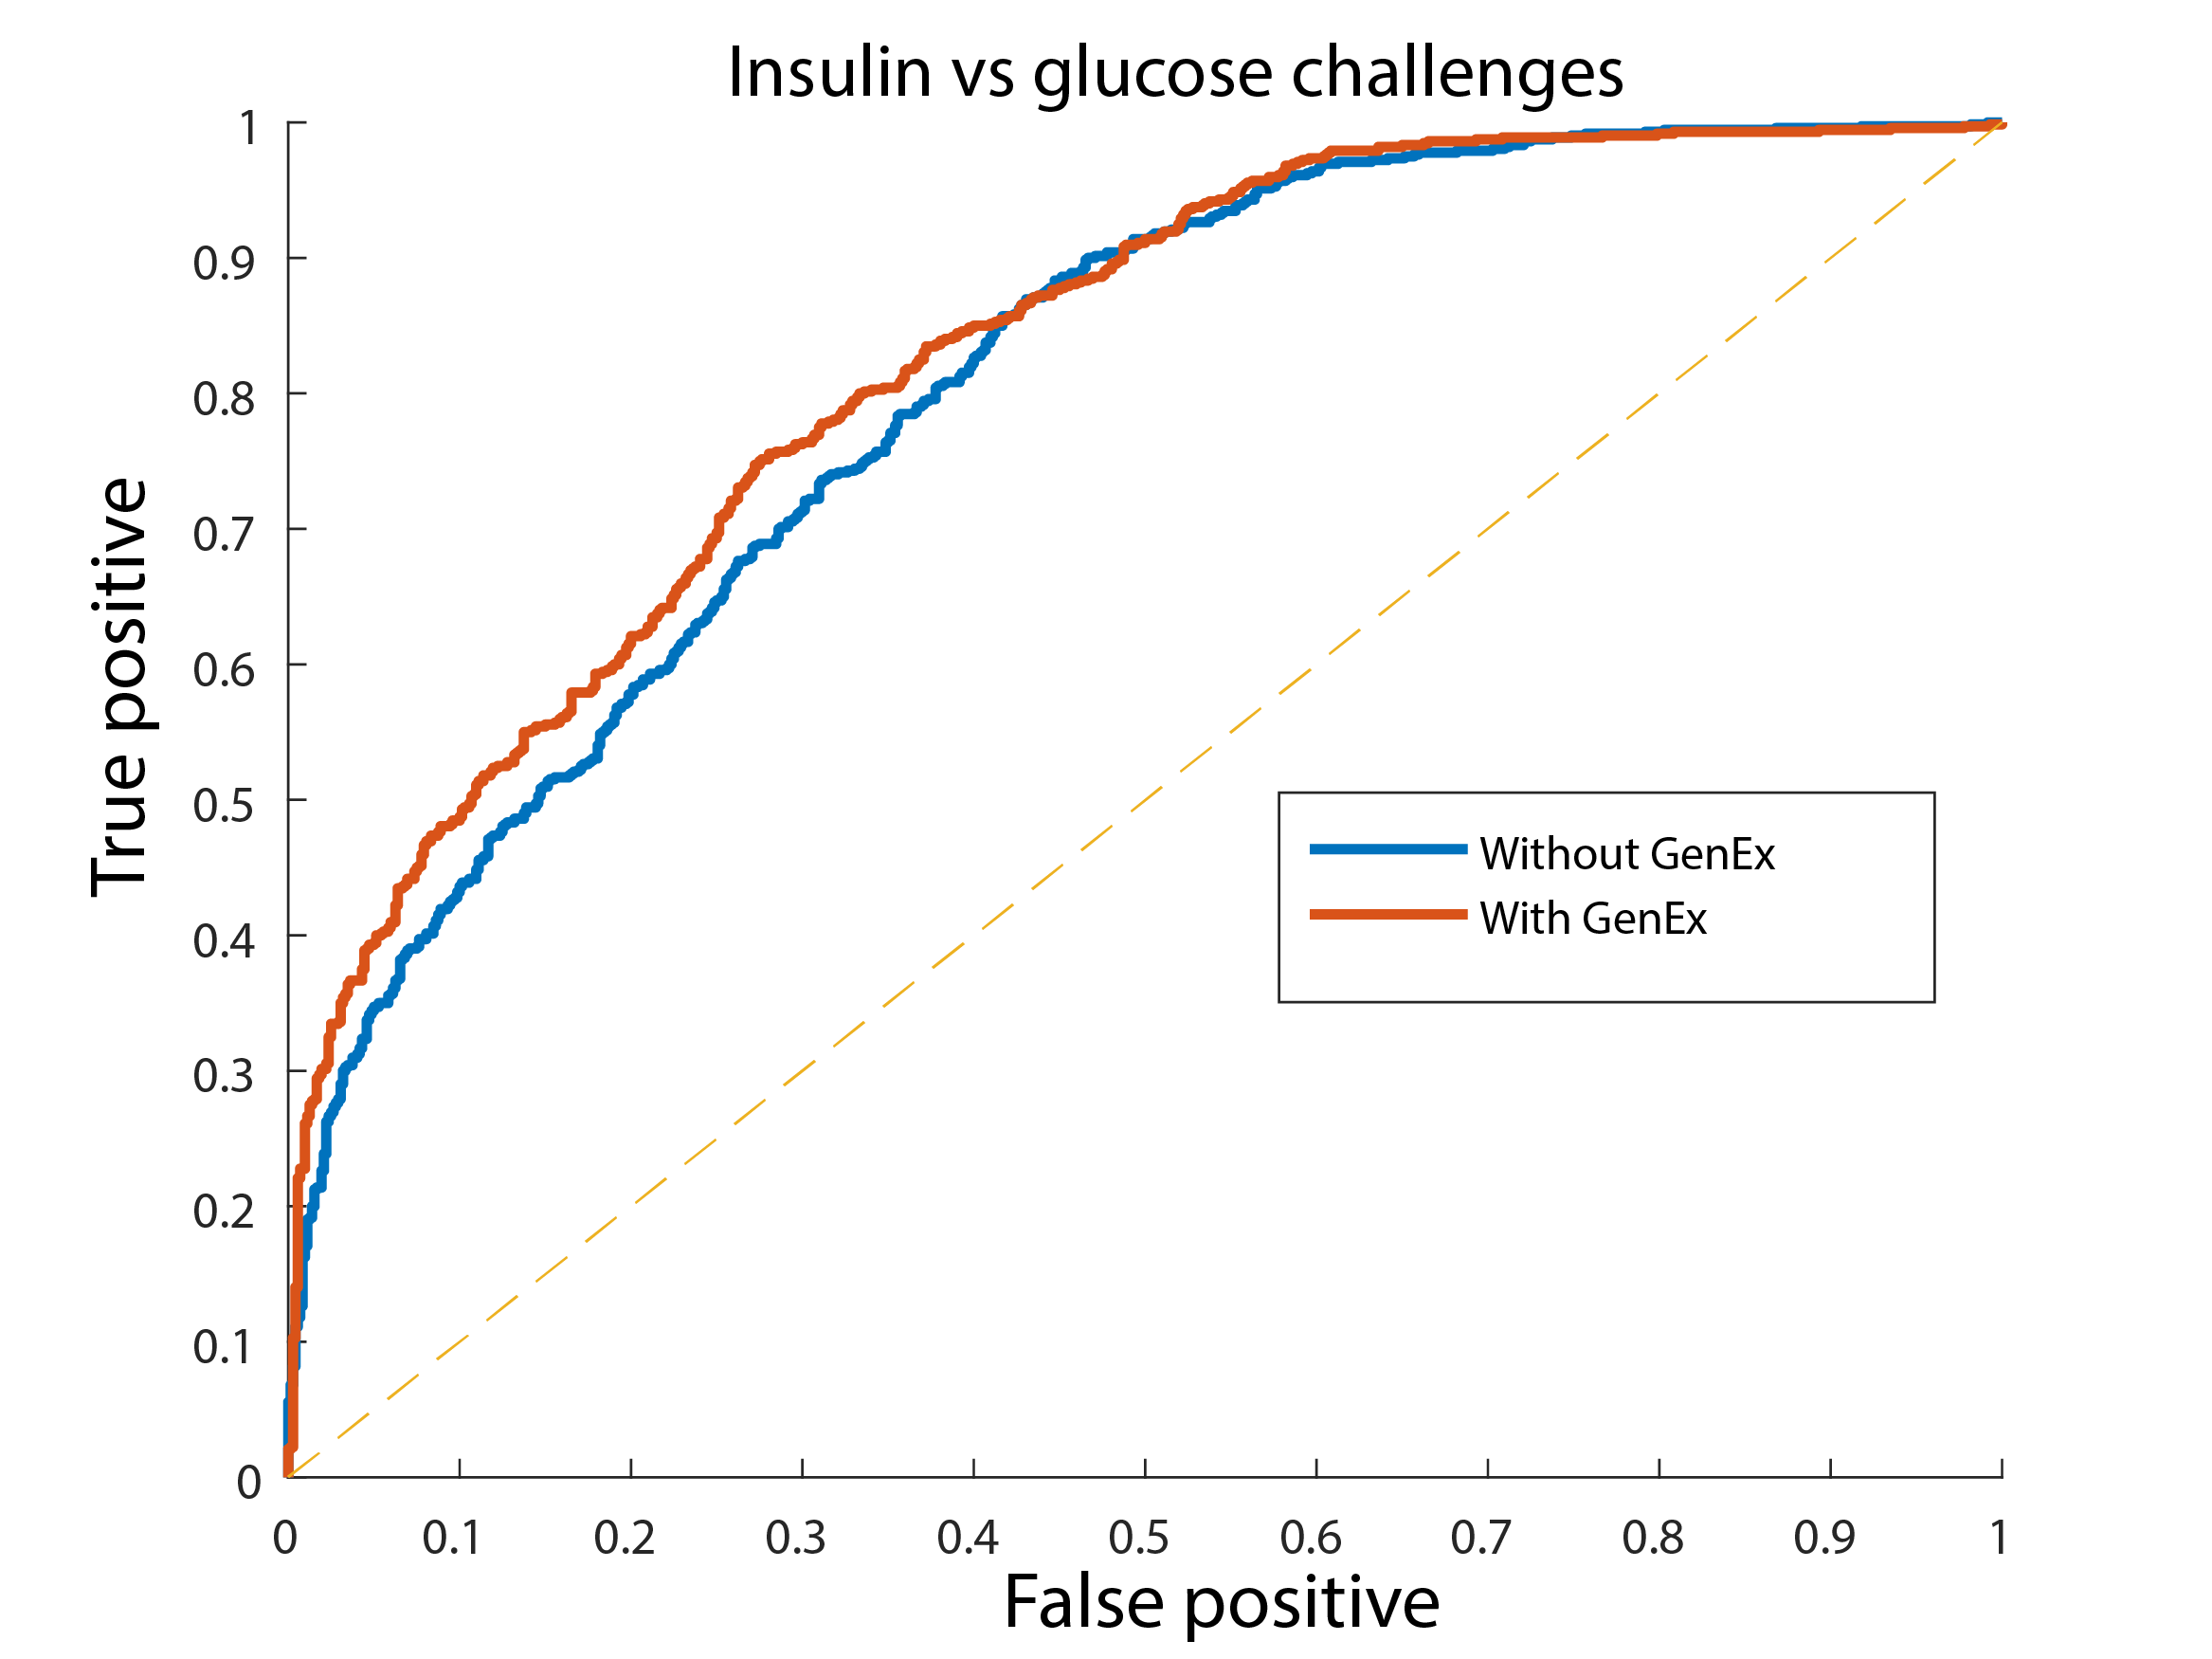
\includegraphics[width=\textwidth,height=\textheight,keepaspectratio]{GIM/figureSX.png}%Figure from images\Figure1.png
	\caption[Whole-body fluxes discriminate between insulin and glucose challenges.]{Whole-body fluxes discriminate between insulin and glucose challenges. A binary class support vectors machine accurately classifies insulin and glucose challenges using whole-body-fluxes. Constraining the model with T1D gene expression further improves the classification result. Insulin challenges were used as the true class.}
	\label{fig:s1GIM}
\end{figure}
\subsection{Relaxing infeasible problems} \label{GIM:sp2}
Subjecting dynamical model-derived constraints to the metabolic model could result in unfeasible problems. The situation could arise from conceptually different modeling approaches. In fact, the GIM model depicted short time events, while the constraint-based model was designed to simulate steady states. For instance, while it is commonly known that organs such as the lungs are glucose metabolizers rather than consumers, the GIM model could show a small secretion of glucose for a short time step as a consequence of free diffusion through the organ membrane. We relaxed the corresponding reactions in Harvey in order to obtain a feasible model through minimally relaxing the upper and lower bounds of the internal reactions. If the standard linear program is infeasible:\\
\begin{alignat*}{2} 
  & \text{max: } &  & c^{T}v\\
  & \text{subject to: } &  &  
                \begin{aligned}[t] \\
                & Sv=0 \\
                & v_{min} \leq v  \leq  v_{max}
                \end{aligned}
\end{alignat*}
, where $c^{T}.v$ is the objective function, $v$ is the flux vector of metabolic reactions, $c$ is the vector of objective coefficients, $S_{(m,n)}$ is the stoichiometric matrix linking $m$ metabolites and $n$ reactions, $lb$ is the vector of reaction lower bound, and $ub$ the vector of reaction upper bound. The following problem minimally relaxes the infeasible model:
\begin{alignat*}{2} 
  & \text{min: } &  & ||p||_{1},||q||_{1}\\
  & \text{subject to: } &  &  
                \begin{aligned}[t] \\
                & Sv=0 \\
                & v_{min} - p \leq v  \leq  v_{max} + q
                \end{aligned}
\end{alignat*}
,where $p$ is the relaxation vector of the lower bound and $q$ is the relaxation vector of the upper bound. Minimizing the 1-norm of $p$ and $q$ ensures both sparsity (minimal cardinal of reactions to be relaxed), with minimal total sum of relaxation amplitude.
\begin{figure}[!htp]
\centering
	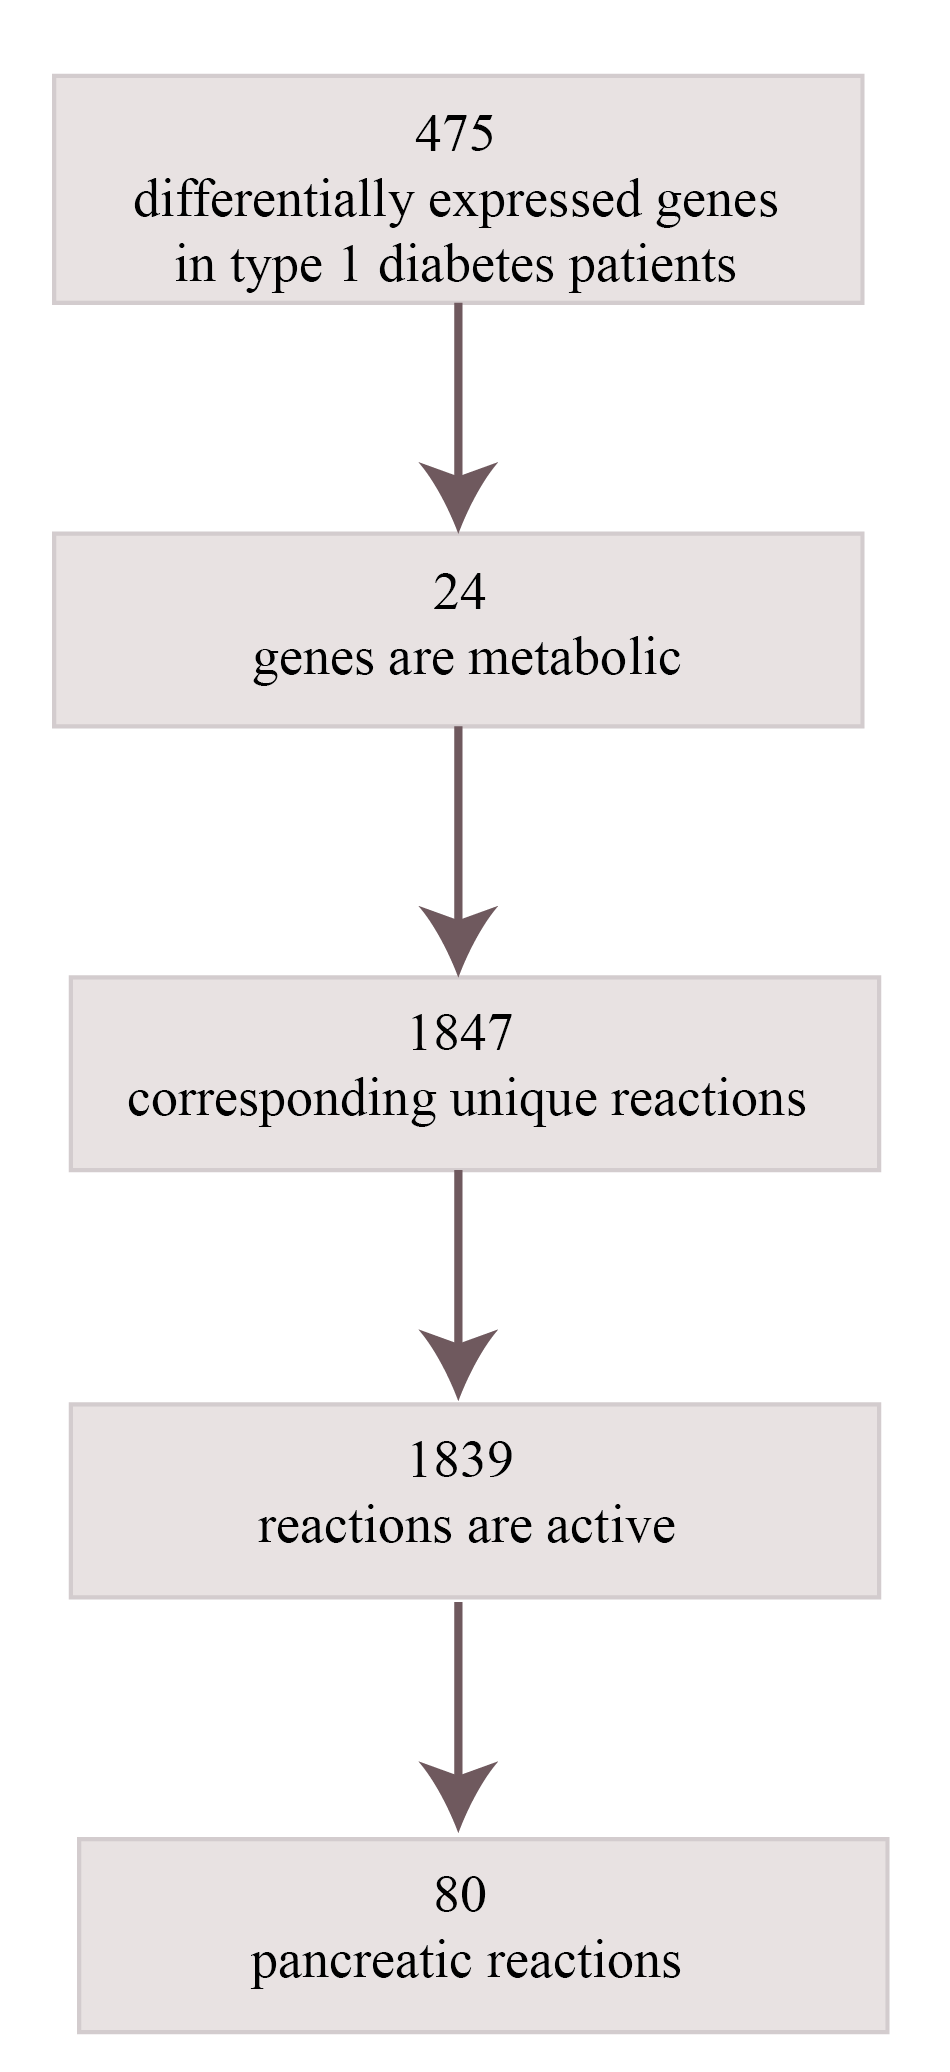
\includegraphics[width=\textwidth,height=\textheight,keepaspectratio]{GIM/figureS2.png}%Figure from images\Figure1.png
	\caption[Gene expression constraints pipeline.]{(Continued on the following page)}
	\label{fig:s2GIM}
\end{figure}
\begin{figure}[t]
  \contcaption{Gene expression constraints pipeline. The pancreas and pancreatic islets gene expression profile of type 1 diabetes patients \cite{planas2010gene} were translated into constraints. The reactions catalysed by a protein coded by a given gene are constrained by the lower and upper bound of gene expression fold change with respect to the control.}% Continued caption
\end{figure}
\subsection{CRONICS framework} \label{GIM:sp3}
The simulation of the hybrid model faced challenges related to 
\begin{itemize}
\item	The the size of the solution space in every time step and the effect of alternate optimal solutions, the problem being largely under-determined.  
\item	Also, the large size of the metabolic model required the reduction of the set of active reactions for subsequent analysis and biological interpretation. 
\item	Simulation time as a model would typically run in 2-3 days for 10 hours of simulation.
\end{itemize}
The above-mentioned challenges were addressed through combining a mosaic of existing techniques in the CRONICS framework which consists of the following steps:\\
\begin{enumerate}
\item	(optional) Depending on the simulation, the solution basis of the unconstrained problem is generated before coupling both the dynamical and metabolic model. The solution basis is then provided in all subsequent optimisation problems while activating the advanced start option in CPLEX as follows:\\
\begin{center}
ADVIND=1
\end{center}
\item	The setting starts with the simulation of dynamical model for 1 time step. Based on dFBA, The computed constraints are subjected to the metabolic model and a 1-norm minimal (pFBA) solution is selected given its sparse properties that allow for the selection of a smaller set of active reactions for further analysis.
\item	(Vertical coupling) The next time step in the dynamical model is simulated and the constraints are computed and subjected to the metabolic model. The selected solution is the one that is minimally distant to the previous solution (MOMA). This part allows to guarantee smoothness of the hybrid system, and the chronology of the simulation. Although the large size of the solution vector made the simulation computationally expensive, we chose a subset of the vector to minimize for. The minimal subset would be the coupled reactions themselves, in this case, the obtained vector is indeed nearly identical to the initial subset vector, which results in all simulations being converging to the dynamical model behaviour in terms of smoothness, while uncoupled reactions can be changing values abruptly in time steps as small as five minutes. While a subset containing reactions of the brain, liver, kidney, adipocytes, muscle, pancreas allowed to globally constrain the fluxes with respect to chronology of simulation while maintaining the smoothness of the system.
\item	(Horizontal coupling) In this previous setting the hybrid model consisted of a dynamically constrained metabolic network. In the horizontal setting, the dynamical model is in return constrained by the metabolic model. The obtained fluxes from the metabolic model serve as input for the next time step of the dynamical model. If the solution fluxes correspond to the input constraints then the hybrid model reaches the behaviour of the dynamical model alone. In both settings, the solution of the type 1 diabetes model in the first time step is minimally distant to the healthy model in the first time step.
\end{enumerate}
We used the CRONICS framework to predict metabolite concentrations in dHarvey model. The metabolites fell under two categories: the metabolites time-course predicted by GIM and the metabolites in Harvey that obey the steady-state assumption. Only the concentrations of imbalanced metabolites in Harvey can be predicted as they do not obey the steady-state assumption. We created demand reactions, which are imbalanced reactions, for metabolites of interest to predict the dynamic organ demand in these metabolites. We applied this method to predict the time-course of ATP demand in the liver (Figure \ref{fig:GIM2}-B), the triglyceride demand in the adipocytes (Figure \ref{fig:GIM3b}), and the valine and phenylalanine demand in plasma (Figure \ref{fig:GIM3a}).
\subsection{Software and solver parameters} \label{GIM:sp4}
The simulations were carried on MATLAB (2014b, Natick, MA, USA) with the ODE15s built-in function and with the COBRA toolbox v3.0 \cite{heirendt2017creation}  and the CPLEX and MAD TOMLAB v7.9 implementation on Windows 7 professional and ubuntu 16.04 –based high performance computing units.
The following parameters allowed a faster convergence as well as resolving ‘infeasbile after unscaling’ type of issues:\\
\begin{center}
PARALLEL=1\\
THREADS=2\\
SCAIND= -1\\
EPMRK=0.9 \\
NUMERICALEMPHASIS=1 \\
EPOPT=1e-6 \\
EPRHS=1e-6 \\
\end{center}
\subsection{Differentially expressed fluxes between healthy and type 1 diabetic models} \label{GIM:sp5}
\begin{figure}[!htp]
\centering
	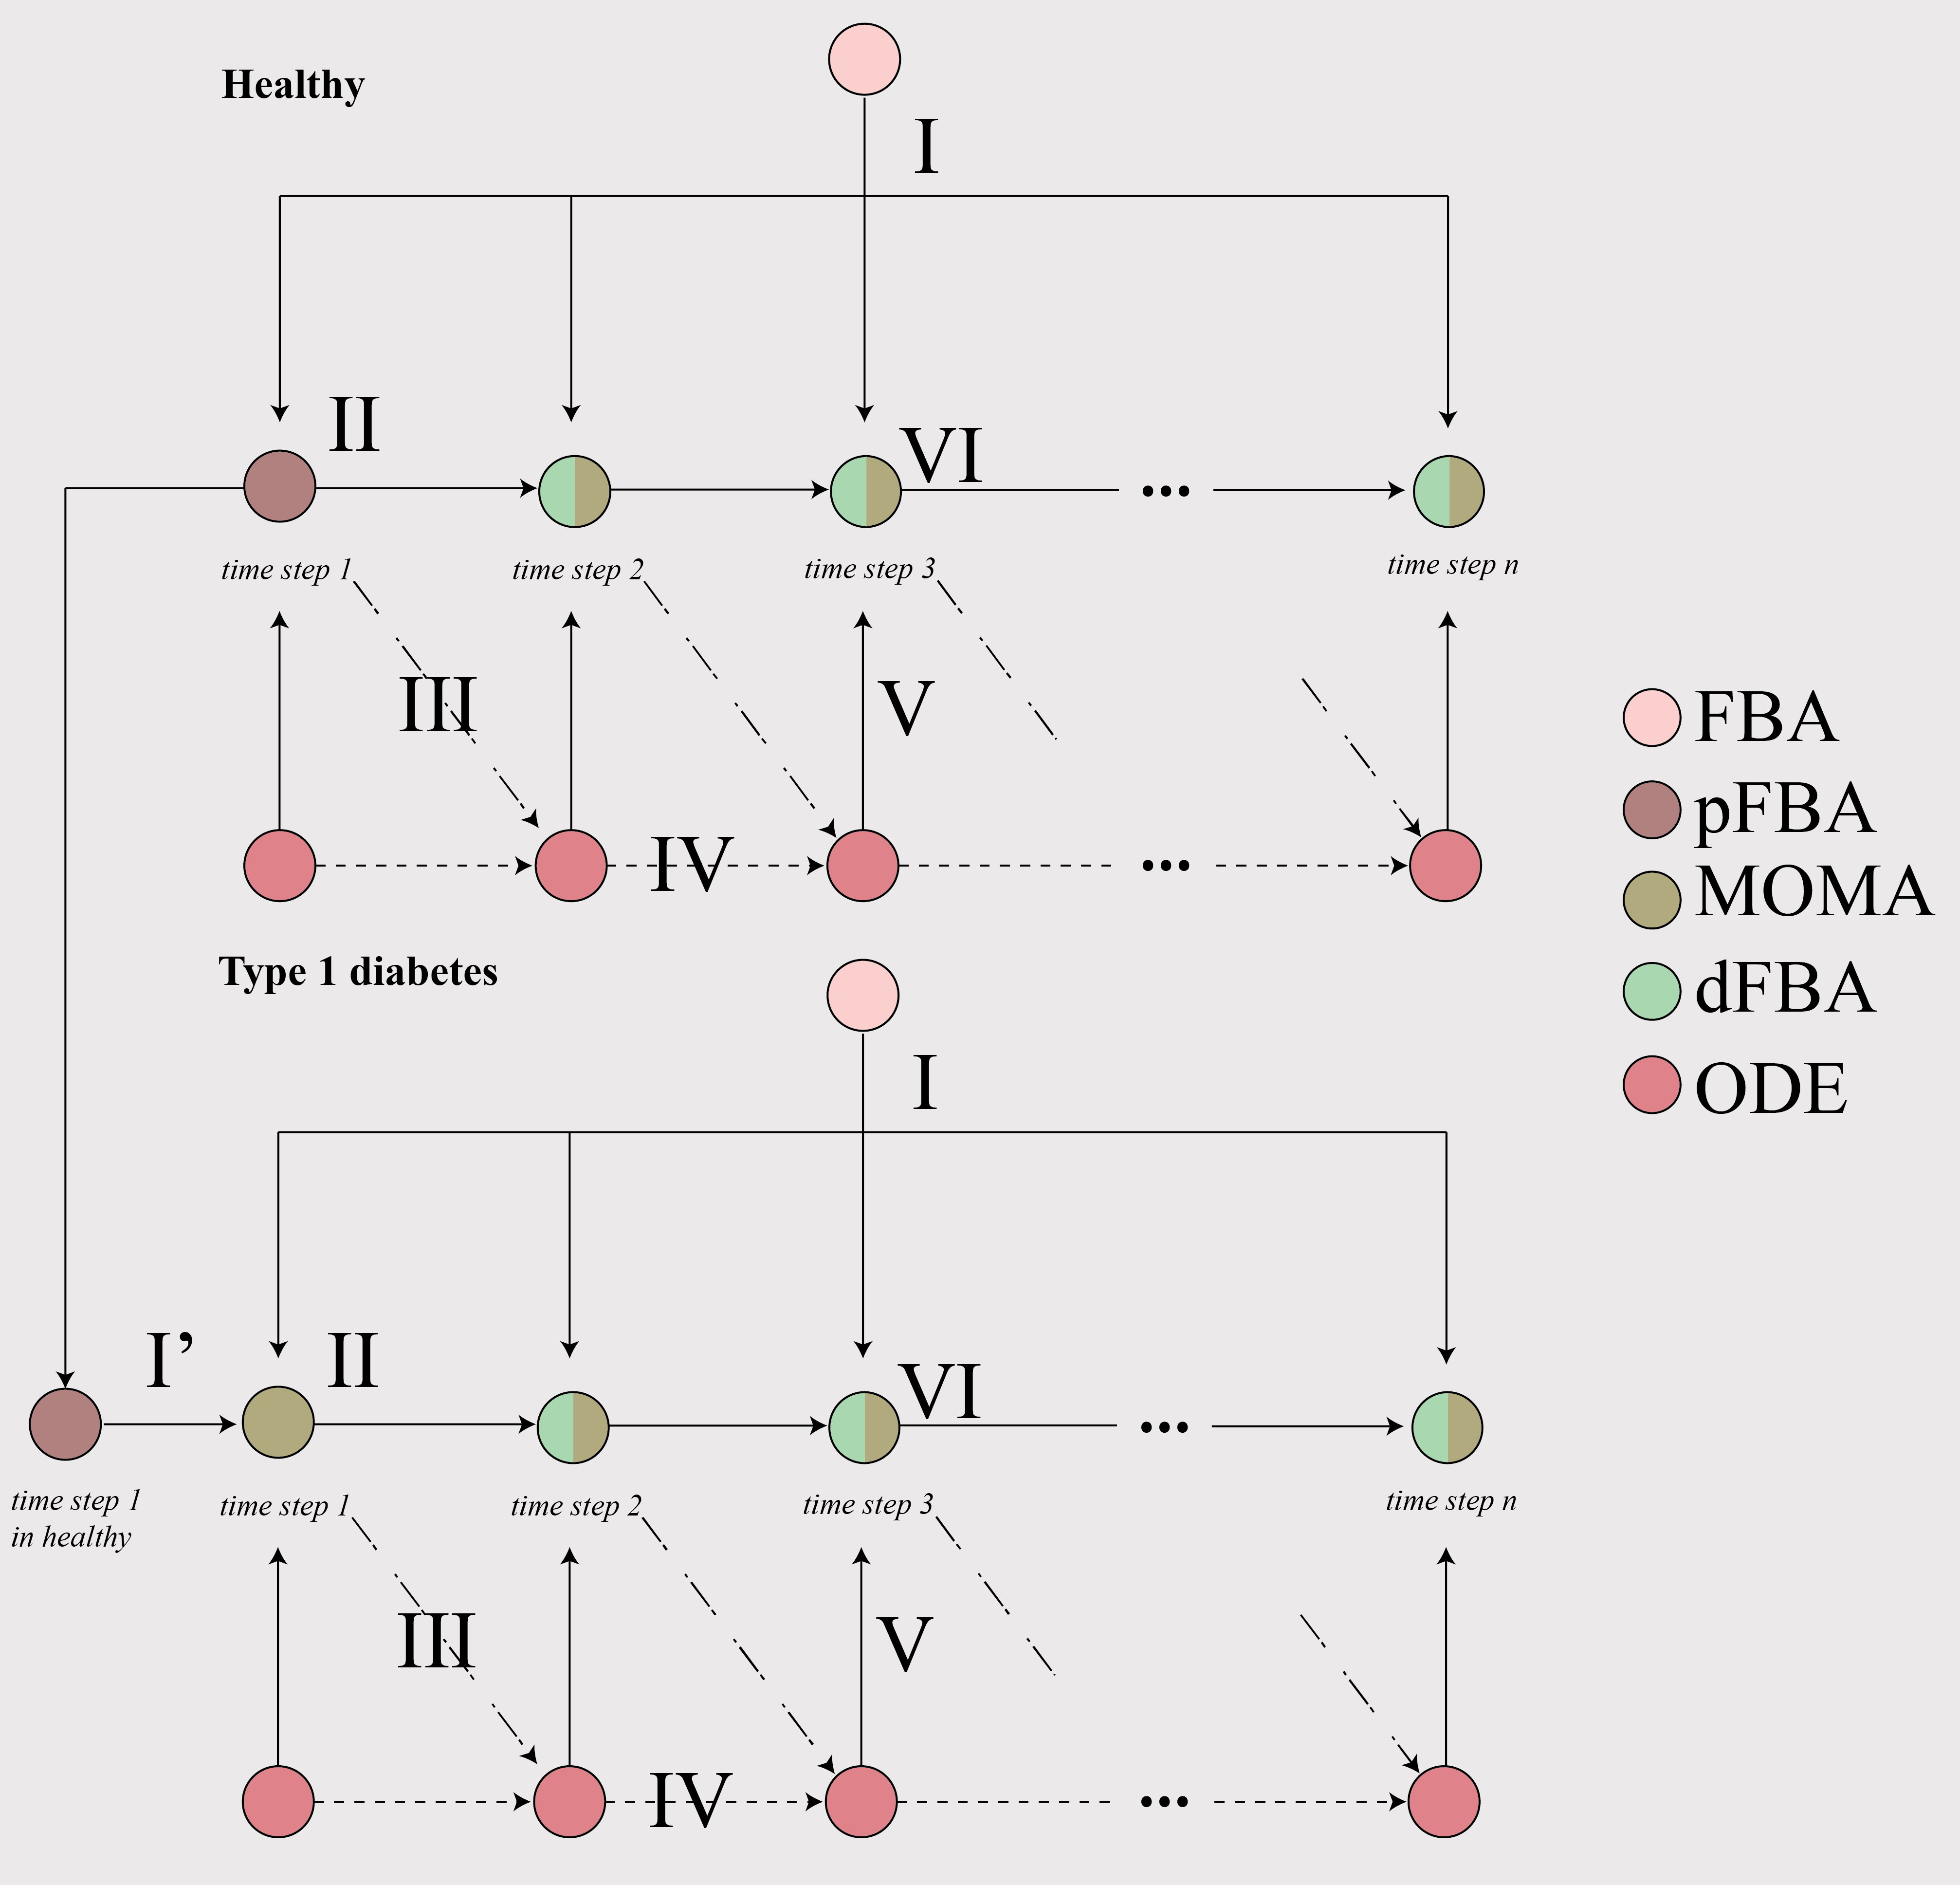
\includegraphics[width=\textwidth,height=\textheight,keepaspectratio]{GIM/figureS3.png}%Figure from images\Figure1.png
	\caption[CRONICS framework for dynamical simulation of genome scale models.]{CRONICS framework for dynamical simulation of genome scale models. The algorithm starts with solving the I) general unconstrained problem with FBA and using its solution basis as a warmstart for the next time steps. II) The first time step is then solved using pFBA after subjecting constraints from the dynamical model to ensure the sparsity of all subsequent solutions. Depending on the type of coupling, the algorithm would either use the constrained-based III) solution as initial estimate for the next time step of the dynamical model to obtain IV) new derivatives that will be subjected on the V) constrained-based model. Alternatively, the dynamical model is independent from the constraint-based model and feedback is only unidirectional (V but not III). The LP problem in the new time step will get constraints from the corresponding time step of the dynamical model, and VI) it will also be constrained by the previous time step so that solutions are minimally distant (MOMA). In type 1 diabetes, the first time step is further constrained by the first time step of the healthy model (I’), in order to ensure a minimal metabolic adjustment between the conditions. Initializing the simulations with pFBA solutions that are minimal to the healthy condition allows to propagate both the sparsity and the minimal metabolic adjustment to the healthy model to all the time steps. The CRONICS framework guarantees a smooth, continuous evolution of the system and reduces the effects of alternate optimal solutions on the predictions.}
	\label{fig:s3GIM}
\end{figure}
In order to compare the fluxes in both healthy and type 1 diabetic model, individual fluxes' comparison would yield inaccurate results given the large alternative optimal solution space. We compared flux distributions per reaction rather than the value provided by one solution. In order to obtain flux probability distributions, we performed flux variability analysis on both healthy and type 1 diabetic model. The COBRA toolbox function \textit{fastFVA} \cite{gudmundsson2010computationally} was called with the solutions as an output as following:\\
\begin{center} 
\textit{{[}minFluxH,maxFluxH,optsolH,retH,fbasolH,fvaminH,fvamaxH{]}=fastFVA(harveyIrrev,\\90,'max','cplex',harvey.rxns,'A',cpxControl)} \\
\end{center}
Prior to the flux variability analysis, the metabolic model was translated to its irreversible version, such as every reversible reaction is decomposed in the forward and the backward reaction, in a way that fluxes obtained are positive. The conversion was done using the following COBRA toolbox function:\\
\begin{center}
\textit{{[}harveyIrrev,matchRev,rev2irrev,irrev2rev{]}
=convertToIrreversibleCoupled(harvey)}\\
\end{center}
The obtained flux distribution per reactions equalled 160320 sample per reaction (80160 reaction* 2 (minimization and maximization)). The two matrices containing the fluxes values per reaction in healthy and type 1 diabetic model were used as an input to volcano plot function \textit{mavolcanoplot} in MATLAB (2014b, Natick, MA, USA). A p-value less than 0.001 was considered as a significance threshold for a minimal fold change of 1.3. Higher values of fold change are usually used in gene expression experiments, with the objective of containing small value change that is related to the experimental set up among several factors. As these considerations do not apply to linear programs solutions, provided the same solver settings, we considered a smaller fold change value.
\subsection{Enrichment of gene vectors}
After obtaining the up-regulated and down-regulated fluxes in T1D, we connected the reactions to their encoding genes and performed gene set enrichment analysis. The set of obtained genes would correspond experimentally to the differentially expressed genes and we queried i) the LINCS database to look for small molecules that reverse the signature of T1D, meaning the compound that induce a reverse genetic signature to the T1D signature that we obtained, which can potentially reverse the metabolic profile and ii) we queried the KEGG database to assess which disease were similar in signature to T1D.\\
In order to determine potential small molecules that can reverse T1D, we collected the list of up-regulated and down-regulated genes in T1D and queried the LINCS Canvas Browser \cite{duan2014lincs}, setting the up-regulated genes and down-regulated genes in the up and down field respectively and using the \textit{reverse} option to look for small molecule that reverse the queried signature. The results are reported in table \ref{GIM:tbls6}.\\
To determine the diseases that have a similar genetic signature to T1D, we merged the up-regulated and down-regulated reactions into a unique set of differentially expressed reactions. Since one metabolic reaction can be encoded by one or more genes using boolean operations (AND, OR), there can be several genetic profiles corresponding to a single metabolic profile. We randomly selected 10,000 genetic profile corresponding to the metabolic profile of T1D and queried each one of them programmatically in Enrichr \cite{chen2013enrichr} through the API. Subsequently, we selected the top five most enriched terms in the KEGG database at p<0.05 for each of the 10,000 gene profiles. Then we ranked the terms by their occurrence in each profile (Figure \ref{fig:sx2GIM}). An example of the output of the enrichment of one profile is listed in table \ref{GIM:tbls5}.\\
The enrichment of metabolic reactions in organs and subsystems as groups was done through a one-sided hypergeometric test with FDR correction. 
%The results are in//metabolic disease PD AD
\begin{figure}[!htp]
\centering
	\includegraphics[width=\textwidth,height=\textheight,keepaspectratio]{GIM/figureSX2.png}%Figure from images\Figure1.png
	\caption[Enrichment of gene expression profiles in KEGG.]{Enrichment of gene expression profiles in KEGG. A- The process of deriving gene profile form metabolic profiles and B- its application to T1D. The identification of differential reaction fluxes in T1D allows to link back to the encoding genes. Since several genes can encode for the same reaction through AND, OR rules in the metabolic model, there can be several differential gene (G) profiles corresponding to one metabolic profile. We sampled 10000 profiles corresponding to the T1D profile and queried KEGG through Enrichr \cite{chen2013enrichr} for each of the profiles (P). The enriched terms (T) for each profile were classified by their occurrence in the 10000 profiles.}
	\label{fig:sx2GIM}
\end{figure}
\subsection{Comparison of flux density estimates}
In order to determine the metabolic effects of insulin in T1D (Figure \ref{fig:GIM3}), we first computed the alternate optimal solutions in T1D model prior to insulin injection, using FVA. We obtained 160032 solutions of the AOS of T1D model, which gives us as many number of flux values per reaction. Using the empirical flux values per reactions, we estimated the smoothed probability density function for each reaction. In a similar fashion, we collected solutions from the T1D model after the SCIB trial and equally, we estimated the probability density of flux values for each reaction. Finally, both density estimates were overlaid in order to compare the effect of insulin on the selection of flux values per enzyme/reaction.
\subsection{Intra-individual variability to insulin response}
We modelled the inter-individual variability to insulin response as the variation of kinetic parameters in GIM model. Consequently, We created 31 GIM model and coupled them to Harvey. The glucose concentrations are completely determined by the GIM model, also referred to as indirect coupling \cite{krauss2012integrating}.\\
Modeling the intra-individual variability to insulin consisted of using the average patient kinetic parameters in GIM and the variation of the internal state of the system as represented by Harvey. In this case, we randomly selected 1\% of reactions in every subsystem in every organ which resulted in a set of 2817 reactions that equally represented all the metabolic subsystems in all the organs. We assigned each reaction a random objective weight which corresponded to a metabolic state. Consequently, we created 31 metabolic state and simulated the models after the subcutaneous injection of insulin. Glucose concentrations are depend on both Harvey and GIM, also referred to as direct coupling \cite{krauss2012integrating}. The input matrix $X_{p,q}$ represents the objective coefficients of each of the $q$ reactions in the $p$ metabolic states. Here, $p=31$ and $q=2817$. The output matrix $Y_{p,n}$ represents the glucose concentrations at each of the $n$ time steps in the $p$ metabolic states, with $n=234$ with a 2.5 minutes time step length and the infusion starting at 16 minutes, totalling 10 hours of simulation. Using multivariate regression, we estimated the matrix $\rho_{q,n}$ that represents the sensitivities of each of the $q$ reactions towards each of the $n$ time steps of the simulation. In particular, the time steps corresponding to the minimal concentration $C_{min}$ and the final concentration $C_{final}$ were considered for further analysis, as they would link to hyperglycaemia and hypoglycaemia and diabetes control in general. The estimation of the sensitivity matrix consisted of solving the following equation:
\begin{gather*}
X* \rho \approx Y \\
\end{gather*}
We used the \textit{mvregress} routine in MATLAB and the Covariance Weighted Least Square (CWLS) algorithm to estimate $\rho$. The algorithm gives $p$ coefficients corresponding to $p$ out of $q$ reactions, wherein the rest in set to zero.
\begin{figure}[!htp]
\centering
	\includegraphics[width=\textwidth,height=\textheight,keepaspectratio]{GIM/figure3a.png}%Figure from images\Figure1.png
	\caption[Effect of insulin on LNAA concentrations.]{Predicted off-target effects on liver glycolytic enzymes and plasma large and neutral amino acids concentration (LNAA) after insulin subcutaneous administration.}
	\label{fig:GIM3a}
\end{figure}

\begin{figure}[!htp]
\centering
	\includegraphics[width=\textwidth,height=\textheight,keepaspectratio]{GIM/TGdynamics.png}%Figure from images\Figure1.png
	\caption[Time-course of triglycerides in the adipocytes.]{Time-course of triglycerides in the adipocyte.}
	\label{fig:GIM3b}
\end{figure}

\begin{figure}[!htp]
\centering
	\includegraphics[width=\textwidth,height=\textheight,keepaspectratio]{GIM/figure3c.png}%Figure from images\Figure1.png
	\caption[Insulin induced inter-organ cross-talk.]{Pancreas, kidney, adipocytes, muscle, liver, and brain metabolic crosstalk with and without insulin action.}
	\label{fig:GIM3c}
\end{figure}


\begin{figure}[!htp]
\centering
	\includegraphics[width=\textwidth,height=\textheight,keepaspectratio]{GIM/figureS4.png}%Figure from images\Figure1.png
	\caption[Variation of the power law gamma across patients after a subcuetanous insulin injection.]{Variation of the power law gamma across patients after a subcutaneous insulin injection. For every patient, the changes of the metabolic network topology were assessed through fitting the metabolite-centric model connectivity on a power law. The variation of the gamma parameter during the simulation time was represented in the boxplot. Overall, the network structure is quite stable across patients and the gamma parameter mean value stays between 3.1 and 3.2 as reported for biological networks \cite{ravasz2002hierarchical}.}
	\label{fig:s4GIM}
\end{figure}

\begin{table}[h]
\caption[Selected metabolic reactions with the highest sensitivities towards peripheral glucose concentrations.]{Selected metabolic reactions with the highest sensitivities towards peripheral glucose concentrations. Type refers to interface reactions (I) shared by Harvey and GIM, and (H) for the reactions belonging to Harvey alone. The letters in brackets refer to the cellular compartments, where e is exrtacellular, c for cytoplasm, m for mitochondria, n for nucleus, and r for endoplasmic reticulum}
\begin{center}
	\begin{tabular*}{\textwidth}{l @{\extracolsep{\fill}} ll}
	\hline
	Name/Type  & Reaction & Subsystem       \\ 
	\hline
	Glut4(I)                   & na1[e]+glc\_D[e] $\leftrightarrow$ na1[c]+glc\_D[c] & Transport      \\
	NMNATr(H)                      & atp[c]+h[c]+nmn[c] $\leftrightarrow$ nad[c]+ppi[c] & NAD metabolism         \\
	GF6PTA(H)            			& f6p[c]+ gln\_L[c] $\rightarrow$ gam6p[c]+glu\_L[c] & Aminosugar metabolism         \\
	TRPO2(H)             			& o2[c]+trp\_L[c] $\rightarrow$ Lfmkynr[c] & Tryptophan metabolism        \\
    HMR\_1280(H)          			& CE4988[c]+nadp[c] $\leftrightarrow$  & Leukotriene metabolism       \\
    & CE5944[c]+h[c]+nadph[c] &\\
	SPODMm(H)            			& 2 h[m]+ 2 o2s[m] $\rightarrow$ h2o2[m]+o2[m] & ROS detoxification        \\
	GUAPRT(H)            			& gua[c]+prpp[c] $\rightarrow$ gmp[c]+ppi[c] & Nucleotide salvage pathway        \\
	DTMPKm(H)            			& atp[m]+dtmp[m] $\rightarrow$ adp[m]+dtdp[m] & Pyrimidine synthesis        \\
	PPNCL3(H)           			& 4ppan[c]+atp[c]+cys\_L[c] $\rightarrow$  & CoA synthesis      \\
	                                & 4ppcys[c]+amp[c]+h[c]+ppi[c]             & \\
	GGT\_L(H)             			& 17.6 ipdp[c]+ttc\_ggdp[c] $\rightarrow$ & N-glycan synthesis        \\
	                                &  0.1 dedoldp\_L[c] + 17.6 ppi[c] & \\
	EX\_ha(e)(H)          			& ha[e] $\leftrightarrow$ & Exchange/demand reaction       \\
	r0301(H)             			& atp[c]+nh4[c]+xmp[c] $\rightarrow$ & Bile acid synthesis        \\
	                                & amp[c]+gmp[c]+2 h[c]+ppi[c] & \\
	PAN4PP(H)            			& h2o[c]+pan4p[c]$\rightarrow$ pi[c]+ptth[c] & CoA catabolism       \\
	RE2235R(H)           			& estrone[r]+h[r]+nadph[r]+o2[r] $\rightarrow$ & Androgen and estrogen        \\
	                                &  C05300[r]+h2o[r]+nadp[r]                    & synthesis and metabolism \\
	IPDDI(H)             			& ipdp[c] $\leftrightarrow$ dmpp[c] & Squalene and cholesterol         \\
	 & &  synthesis\\
	DASCBR(H)            			& dhdascb[c]+nadph[c] $\rightarrow$ ascb\_L[c]+nadp[c] & Vitamin C metabolism        \\
	r0009(H)             			& h2o[x]+ppi[x] $\rightarrow$ h[x]+2 pi[x] & Purine metabolism      \\
	SBTR(H)             			& glc\_D[c]+h[c]+nadph[c] $\rightarrow$ nadp[c]+sbt\_D[c] & Fructose and mannose         \\
	& & metabolism\\
	RE1303C(H)           			& h[c]+nadph[c]+o2[c]+vitd3[c] $\rightarrow$   & Vitamin D metabolism      \\
	                                & 25hvitd3[c] + h2o[c] + nadp[c]               &\\
	r2073(H)             			& h[e]+zn2[e] $\rightarrow$ h[c]+zn2[c] & Transport, extracellular        \\
	EX\_icdchol(H)        			& icdchol[e] $\leftrightarrow$ & Exchange/demand reaction       \\
	EX\_CE2934(e)(H)      			& CE2934[e] $\leftrightarrow$ & Exchange/demand reaction        \\
	P4507A1r(H)          			& chsterol[r]+h[r]+nadph[r]+o2[r] $\rightarrow$ & Bile acid synthesis        \\
	                                & h2o[r]+nadp[r]+xol7a[r] & \\
	RAtn3(H)             			& 13\_cis\_retn[c] $\leftrightarrow$ 13\_cis\_retn[n] & Transport, nuclear       \\
	\hline
	\end{tabular*}
\end{center}
\label{GIM:tblsRxn}%descriptive label to refer to figure in text
\end{table}%Path to supplementary material

\end{document}
